\documentclass{icthesis}

\usepackage{etex}

\usepackage{array,booktabs,epsfig,lmodern,pstricks,subfig,textcomp}

\newcommand{\R}{\mathbb R}
\newcommand{\D}{\mathcal D}
\newcommand{\W}{\vec{\mathcal W}}
\newcommand{\vol}{\mathcal{L}^d}
\newcommand{\surfvol}{\mathcal{H}^{d-1}}
\newcommand{\dH}[1]{\;{\rm d}{\cal H}^{#1}} % Hausdorff measure
\newcommand{\dL}[1]{\;{\rm d}{\cal L}^{#1}} % Lebesgue measure
\newcommand{\bigchi}{\ensuremath{\mathrm{\mathcal{X}}}}
\newcommand{\charfcn}[1]{\bigchi_{#1}} % characteristic function
\newcommand{\Vh}{\underline{V}(\Gamma^m)}
\newcommand{\Wh}{W(\Gamma^m)}
\newcommand{\Vht}{\underline{V}(\Gamma^h(t))}
\newcommand{\Wht}{W(\Gamma^h(t))}
\newcommand{\uspacesimple}{\mathbb{U}}
\newcommand{\uspace}[1]{\mathbb{U}(\vec{#1})}
\newcommand{\uspacedisc}[2]{\mathbb{U}^{#2}(\vec{#1})}
\newcommand{\pspace}{\mathbb{P}}
\newcommand{\pnormspace}{\widetilde\pspace} % normalized pressure space
\newcommand{\uspacesimpleref}{\mathcal{U}} % ale reference space
\newcommand{\uspaceref}[1]{\mathcal{U}(\vec{#1})} % ale reference space
\newcommand{\uspacesemidiscref}[3]{\mathcal{U}^{#2}(\vec{#1},#3)}
% ale reference space
\newcommand{\pspaceref}{\mathcal{P}} % ale reference space
\newcommand{\pnormspaceref}{\widetilde\pspaceref}% ale reference space
\newcommand{\uspacesimpleale}{\mathfrak{U}} % ale space
\newcommand{\uspaceale}[1]{\mathfrak{U}(\vec{#1})} % ale space
\newcommand{\uspacesemidiscale}[3]{\mathfrak{U}^{#2}(\vec{#1},#3)} % ale space
\newcommand{\uspacediscale}[2]{\mathfrak{U}^{#2}(\vec{#1})} % ale space
\newcommand{\pspaceale}{\mathfrak{P}} % ale space
\newcommand{\pnormspaceale}{\widetilde\pspaceale}% ale normalized space
\newcommand{\kspace}{\mathbb{K}}
\newcommand{\xspace}{\mathbb{X}}
\newcommand{\sigmaO}{o}
\newcommand{\nabs}{\nabla_{\!s}}
\newcommand{\id}{\rm id}
\newcommand{\ddt}{\frac{\rm d}{{\rm d}t}}
\newcommand{\NbulkT}{\vec{N}_{\Gamma,\Omega}^T}
\newcommand{\Nbulk}{\vec{N}_{\Gamma,\Omega}}
\newcommand{\errorXx}{\|\Gamma^h - \Gamma\|_{L^\infty}}
\newcommand{\LerrorUu}[1]{\|\vec U - I^h_{#1}\,\vec u\|_{L^2}}
\newcommand{\HerrorUu}[1]{\|\vec U - I^h_{#1}\,\vec u\|_{L^2(H^1)}}
\newcommand{\LerrorPp}{\|P - p\|_{L^2}}
\newcommand{\unitn}{\vec{\rm n}}
\newcommand{\unitt}{\vec{\rm t}}
\newcommand{\mat}[1]{\underline{\underline{#1}}\rule{0pt}{0pt}}
\newcommand{\Rey}{\mbox{\textit{Re}}} % Reynolds number
\newcommand{\V}{\vec{\mathcal{V}}} % surface velocity
\newcommand{\pdg}{${\rm P1}^{{\rm dg}_\Gamma}$} % P1 DG across interface
\newcommand{\strikes}{\mbox{$s\!\!\!\!\:/$}}
\newcommand{\myurl}[1]{\hfil\penalty 100 \hfilneg \hbox{\url{#1}}} % force
% newline before long url

\begin{document}

\captionsetup[subfigure]{labelformat=empty} % remove label subplot
\captionsetup[subfigure]{justification=centering} % center caption subplot

\title{Front tracking finite element methods for two-phase Navier--Stokes flow}
\author{Marco Agnese}
\advisor{Robert N\"urnberg}
\degree{Doctor of Philosophy}
\field{Mathematics}
\degreeyear{2017}
\degreemonth{April}
\department{Mathematics}
%\pdOneName{B.Sc.}
%\pdOneSchool{Politecnico di Torino}
%\pdOneYear{2010}
%\pdTwoName{M.Sci.}
%\pdTwoSchool{Politecnico di Torino}
%\pdTwoYear{2013}

\maketitle
\setstretch{1.2}
\abstractpage
\dedicationpage
\acknowledgments
\listoffigures
\listoftables
\tableofcontents

\mainmatter
\chapter{\sc Introduction}\label{ch:introduction}
Fluid flow problems with an unknown interface are ubiquitous in physics and
engineering. This introductory chapter is devoted to a description of the
mathematical model used to model this type of systems together with a brief
overview of the possible approaches to describe the unknown interface.

The chapter is organised as follows: in \S\ref{sec:free_boundary_flows}
we define what a free-boundary fluid flow is and we introduce a generic setting
for the problem; in \S\ref{sec:flow_equations} we present the
Navier--Stokes equations which govern the fluid; in
\S\ref{sec:bc_conditions} we discuss the boundary, initial and interface
conditions needed for the well possessedness of the problem; in
\S\ref{sec:interface_treatment} we briefly overview the different ways to
treat the unknown interface; in \S\ref{sec:numerical_challenges} we detail
the various numerical challenges posed by these types of flows; in
\S\ref{sec:numerical_implementation} we finally list the libraries used to
implement the numerical schemes described in this thesis and we provide the
links to the code developed in order to make all the results presented in this
work reproducible.

\section{Free-boundary fluid flows}\label{sec:free_boundary_flows}
Fluid flow problems with a moving interface are encountered in many
applications in physics, engineering and biophysics. Typical applications are
drops and bubbles, die swell, dam break, liquid storage tanks, dendritic growth,
ink-jet printing, fuel injection. For this reason, developing robust and
efficient numerical methods for these flows is an important problem and
has attracted tremendous interest over the last decade.

In these type of problems, apart from the flow solution in the bulk domain, the
position of a portion of the boundary is also unknown. This boundary can either
be an external boundary or an interface between sub-domains. At the
boundary/interface, certain boundary conditions need to be fulfilled, which
specify the position of the boundary. These conditions relate the variables of
the flow, velocity and pressure, across the domains under consideration of
external influences, such as for example surface tension. Numerically, in order
to be able to compute the flow solution as well as the boundary/interface
geometry, a measure to track the boundary starting from an initial position
needs to be incorporated.

The scenario we consider are two-phase flows, liquid-liquid or liquid-gas, in a
$d$-dimensional computational domain $\Omega\subset\R^d$. This domain
$\Omega$ contains two different immiscible fluids which, for all $t\in[0,T]$,
occupy time dependent regions $\Omega_+(t)$ and
$\Omega_-(t):=\Omega\setminus\overline{\Omega}_+(t)$ and
which are separated by an interface $(\Gamma(t))_{t\in[0,T]}$,
$\Gamma(t)\subset\Omega$. For later use, we always assume that
$(\Gamma(t))_{t\in [0,T]}$ is a sufficiently smooth evolving hypersurface
without boundary. See Figure~\ref{fig:two_phase_sketch} for an illustration.
\begin{figure}
\begin{center}
\unitlength15mm
\psset{unit=\unitlength,linewidth=1pt}
\begin{picture}(4,4)(0,0)
\psline(0,0)(4,0)(4,4)(0,4)(0,0)
\psline{->}(3,2)(3.5,2)
\pscustom[fillstyle=solid,fillcolor=lightgray!50]
{
\psellipse(2,2)(1,1)
}
\put(3.25,1.75){$\vec\nu$}
\put(1.75,0.75){{$\Gamma$}}
\put(1.75,2){{$\Omega_-$}}
\put(0.5,3.25){{$\Omega_+$}}
\end{picture}
\end{center}
\caption[Two-phase flow]{Two-phase flow setting.}
\label{fig:two_phase_sketch}
\end{figure}
Therefore both the sub-domains themselves and the flow field are part of the
solution. Indeed the main task in this context is to account for the interface
$\Gamma(t)$, which separates the distinct fluid domains and is generally in
motion. Apart from its exact position, the computation of geometrical quantities
of $\Gamma(t)$ such as its normal vector $\vec\nu$ and its mean curvature
$\varkappa$ are of interest.

\section{Flow governing equations}\label{sec:flow_equations}
For what concern the bulk flow, we restrict ourselves to isothermal conditions,
incompressible fluids and we assume that there is no change of phase. Under
this assumption, the fluid dynamics is modelled by the incompressible
Navier--Stokes equations. For more details see \cite{GrossR11}.

Denoting the velocity and pressure by $\vec u$ and $p$, respectively, we
introduce the Newtonian stress tensor
\begin{equation} \label{eq:stress_tensor}
\mat\sigma = \mu \,(\nabla\,\vec u + (\nabla\,\vec u)^T) - p\,\mat\id
= 2\,\mu\, \mat D(\vec u)-p\,\mat\id\,,
\end{equation}
where $\mu(t) = \mu_+\,\charfcn{\Omega_+(t)} + \mu_-\,\charfcn{\Omega_-(t)}$,
with $\mu_\pm \in \R_{>0}$, denoting the dynamic viscosities in the two phases,
$\mat\id \in \R^{d \times d}$ is the identity matrix and
$\mat D(\vec u):=\frac{1}{2}\, (\nabla\vec u+(\nabla\vec u)^T)$
is the rate-of-deformation tensor. Given a vector valued function $\vec
h:\R^d\to\R^d$, we define its gradient as
$\nabla\vec h = ((\nabla h_1)^T;\ldots;(\nabla h_d)^T)$. Moreover, let
$\rho(t) = \rho_+\,\charfcn{\Omega_+(t)} + \rho_-\,\charfcn{\Omega_-(t)}$,
with $\rho_\pm \in \R_{>0}$, be the fluid density.

Imposing the conservation of momentum and mass in each phase, the following
standard Navier--Stokes governing equations can be derived:
\begin{subequations}
\begin{alignat}{2}
\rho\,(\vec u_t +\vec u \,.\, \nabla \vec u)- \nabla\,.\,\mat\sigma
& = \vec f \quad &&\mbox{in } \Omega_\pm(t)\,,
\label{eq:ns_momentum} \\
\nabla\,.\,\vec u & = 0 \quad &&\mbox{in } \Omega_\pm(t)\,,
\label{eq:ns_mass}
\end{alignat}
\end{subequations}
where $\vec f$ includes all external body forces referred to the unit mass of
fluid.

Substituting (\ref{eq:stress_tensor}) in (\ref{eq:ns_momentum}), we obtain the
well known incompressible Navier--Stokes model:
\begin{subequations}
\begin{alignat}{2}
\rho\,(\vec u_t +\vec u \,.\, \nabla \vec u) -2 \mu\,\nabla\,.\,\mat D(\vec u)+
\nabla\,p & = \vec f \quad &&\mbox{in } \Omega_\pm(t)\,,
\label{eq:ns_momentum_bis} \\
\nabla\,.\,\vec u & = 0 \quad &&\mbox{in } \Omega_\pm(t)\,.
\label{eq:ns_mass_bis}
\end{alignat}
\end{subequations}

To better grasp the physical meaning of the terms appearing in the momentum
equation (\ref{eq:ns_momentum_bis}) we briefly describe them. The inertia term
$\vec u \,.\, \nabla \vec u$ is a convection term arising from the conservation
of momentum. The momentum of each portion of fluid needs to be conserved
therefore it needs to move with the fluid which means that it is convected with
the fluid. The pressure term $\nabla\,p$  is originated by the Newtonian
constitutive equation (\ref{eq:stress_tensor}) and it represent all the forces
resulting from pressure differences within the fluid. Finally, the friction
term $\nabla\,.\,\mat D(\vec u)$, which again arises from the Newtonian
constitutive equation (\ref{eq:stress_tensor}), is a diffusion operator
equalizing the velocity of neighbouring elements. The more viscous the fluid,
the stronger is the friction between neighbouring particles and thus the
equalizing effect.

The Reynolds number $\Rey$ is an important dimensionless quantity in fluid
mechanics and it is defined as
\begin{equation}\label{eq:reynolds}
\Rey=\frac{\rho\,u_c\,L_c}{\mu}\,,
\end{equation}
where $L_c$ is the characteristic dimension of the problem and $u_c$ is the
characteristic velocity of the fluid. It quantifies the ratio of inertial
forces to viscous forces within the fluid, therefore it is used to predict
flow patterns in different fluid flow situations. If $\Rey \ll 1$ the flow is
laminar due to the fact that viscous forces are dominant and it is
characterized by smooth, constant fluid motion.  Otherwise, the flow is
turbulent due to the fact that inertial forces are dominant and it tends to
produce chaotic eddies, vortices and other flow instabilities.

In the case of laminar flow, the advective term in the momentum equation
(\ref{eq:ns_momentum}) can be neglected, giving rise to the so called Stokes
equations
\begin{subequations}
\begin{alignat}{2}
- \nabla\,.\,\mat\sigma & = \vec f \quad &&\mbox{in } \Omega_\pm(t)\,,
\label{eq:momentum} \\
\nabla\,.\,\vec u & = 0 \quad &&\mbox{in } \Omega_\pm(t)\,,
\label{eq:mass}
\end{alignat}
\end{subequations}
which for Newtonian fluids are expressed as
\begin{subequations}
\begin{alignat}{2}
-2 \mu\,\nabla\,.\,\mat D(\vec u)+ \nabla\,p & = \vec f \quad &&\mbox{in }
\Omega_\pm(t)\,,
\label{eq:momentum_bis} \\
\nabla\,.\,\vec u & = 0 \quad &&\mbox{in } \Omega_\pm(t)\,.
\label{eq:mass_bis}
\end{alignat}
\end{subequations}

We finally observe that for the one-phase Navier--Stokes flow,
$\rho_+=\rho_-=\rho$ and $\mu_+=\mu_-=\mu$, using the
incompressibility condition (\ref{eq:ns_mass_bis}) we have
\begin{equation}
2\nabla\,.\,\mat D(\vec u) = \nabla\,.\big(\nabla\vec u+(\nabla\vec u)^T\big)=
\Delta \vec u + \nabla(\nabla\,.\vec u) = \Delta \vec u
\end{equation}
therefore the system (\ref{eq:ns_momentum_bis}--b) can be rewritten as
\begin{subequations}
\begin{alignat}{2}
\rho\,(\vec u_t +\vec u \,.\, \nabla \vec u) - \mu\,\Delta\vec u+\nabla\,p
& = \vec f \quad \mbox{in } \Omega\,, \\
\nabla\,.\,\vec u & = 0 \quad \mbox{in } \Omega\,,
\end{alignat}
\end{subequations}
which is the canonical form of the one-phase Navier--Stokes problem.

\section{Boundary, initial, and interface conditions}\label{sec:bc_conditions}
For the full Navier--Stokes problem (\ref{eq:ns_momentum_bis}-b), a
divergence-free velocity field for the whole computational domain is needed as
an initial condition. Therefore we impose
\begin{equation}\label{eq:ns_ic}
\vec u(0) = \vec u_0 \quad \mbox{in } \Omega\,.
\end{equation}
The initial condition is not need in the Stokes case (\ref{eq:momentum_bis}-b)
since it is a stationary problem.

In order to obtain a well-posed system, boundary conditions have to be imposed
on the bulk domain boundary $\partial\Omega$. Let $\partial\Omega$ be
partitioned as $\partial\Omega=\partial_1\Omega \cup \partial_2\Omega$ with
$\partial_1\Omega \cap \partial_2\Omega = \emptyset$. We use the Dirichlet
condition on $\partial_1 \Omega$
\begin{equation}\label{eq:ns_bc_dirichlet}
\vec u = \vec g \quad \mbox{on } \partial_1 \Omega\,,
\end{equation}
and the free-slip condition on $\partial_2 \Omega$
\begin{equation}\label{eq:ns_bc_freeslip}
\vec u \,.\,\unitn = 0  \quad \mbox{on } \partial_2 \Omega\,,
\end{equation}
with $\unitn$ denoting the outer unit normal of $\partial \Omega$. We notice
that the case $\vec g = \vec 0$ corresponds to the so called no-slip condition.

Since we are dealing with a two-phase flow, some interface conditions are also
needed on the unknown interface $\Gamma(t)$, which couple the velocity and
stress between the two domains. Viscosity of the fluids leads to the continuity
condition
\begin{equation}\label{eq:interface_jump_velocity}
[\vec u]_-^+ = \vec 0 \quad \mbox{on } \Gamma(t)\,,
\end{equation}
where $[\vec u]_-^+ := \vec u_+ - \vec u_-$ denote the jump in velocity across
the interface $\Gamma(t)$. Here and throughout, we employ the shorthand notation
$\vec h_\pm := \vec h\!\mid_{\Omega_\pm(t)}$ for a function
$\vec h : \Omega \times [0,T] \to \R^d$; and similarly for scalar and
matrix-valued functions.

The assumption that there is no change of phase leads to the dynamic interface
condition
\begin{equation}\label{eq:interface_velocity}
\V\,.\,\vec\nu = \vec u\,.\,\vec \nu \quad \mbox{on }
\Gamma(t)\,,
\end{equation}
given that $\V$ is the velocity of the evolving interface
$\Gamma(t)$ and where $\vec\nu(t)$ is the unit normal on $\Gamma(t)$ pointing
into $\Omega_+(t)$. Therefore the normal velocity of the interface needs to
match the flow normal velocity across the interface $\Gamma(t)$.

The momentum conservation in a small material volume that intersects the
interface leads to the stress balance condition
\begin{equation}\label{eq:interface_jump_stress_div}
[\mat\sigma\,\vec \nu]_-^+ = -\nabs\,.\mat\sigma_{\Gamma} \quad \mbox{on }
\Gamma(t)\,,
\end{equation}
where $\mat\sigma_{\Gamma}$ is the interface stress tensor and $\nabs\,.$ is
the surface divergence on $\Gamma(t)$. The operator $\nabs$ is the surface
gradient on $\Gamma(t)$ and it is the orthogonal projection of the usual
gradient operator $\nabla$ on the tangent space of the surface $\Gamma(t)$.
Therefore, given a smooth function $h$ defined on a neighbourhood of
$\Gamma(t)$, it is defined as
\begin{equation}\label{eq:surface_gradient}
\nabs\,h(\vec z)=\mat P\,\nabla\,h(\vec z)=\nabla\,h(\vec z)\,-
\,\nabla\,h(\vec z)\,.\,\vec\nu(\vec z)\,\vec\nu(\vec z)\,,\quad \vec z
\in\Gamma(t)\,,
\end{equation}
with the usual projection operator $\mat P$ defined as
\begin{equation}\label{eq:surface_projection}
\mat P(\vec z)=\mat\id\,-\,\vec\nu(\vec z)\,\vec\nu(\vec z)^T\,,\quad \vec
z\in \Gamma(t)\,.
\end{equation}
It can be shown that the definition of $\nabs\,h$ does not depend on the chosen
extension of $h$, but only on the value of $h$ on $\Gamma(t)$. See
\cite{DeckelnickDE05}. For later use, we also define the surface Laplacian, also
known as Laplace--Beltrami operator, $\Delta_s$ on $\Gamma(t)$ as
\begin{equation}\label{eq:surface_laplacian}
\Delta_s = \nabs\,.\,\nabs\,.
\end{equation}

We restrict ourselves to the case that the only force acting on the interface
is the surface tension contact force. Therefore the interface stress tensor
$\mat\sigma_\Gamma$ has the following constitutive equation
\begin{equation}\label{eq:interface_stress_tensor}
\mat\sigma_{\Gamma}=\gamma\,\mat P\,,
\end{equation}
where $\gamma$ is the surface tension coefficient. Substituting
(\ref{eq:interface_stress_tensor}) in (\ref{eq:interface_jump_stress_div}) we
obtain
\begin{equation}\label{eq:interface_stress_tensor_divergence}
\begin{align*}
[\mat\sigma\,\vec \nu]_-^+ &= -\nabs\,.(\gamma\,\mat P)
= -\gamma\,\nabs\,.\,\mat P-\nabs\,\gamma
= \gamma\nabs\,.\,(\vec\nu\,\vec\nu^T)-\nabs\,\gamma \\
& = \gamma\nabs\,.\,\vec\nu\,\vec\nu + \gamma\nabs\,\vec\nu\,.\,\vec\nu
- \nabs\,\gamma = \gamma\nabs\,.\,\vec\nu\,\vec\nu - \nabs\,\gamma \\
& = -\gamma\,\varkappa\,\vec\nu - \nabs\,\gamma \quad \mbox{on } \Gamma(t)\,,
\end{align*}
\end{equation}
where we have used the fact that the surface gradient $\nabs$ is, by definition,
always orthogonal to the surface normal $\vec\nu$ and that $\varkappa =
-\nabs\,.\vec\nu$ is the mean curvature of $\Gamma(t)$. The projection $\mat P$
is used, since $\mat\sigma_{\Gamma}$ should represent only contact forces that
are tangential to the surface. We assume that $\gamma$ is constant and
therefore, from (\ref{eq:interface_stress_tensor_divergence}), we obtain the
so called clean interface model for the interfacial forces
\begin{equation}\label{eq:interface_jump_stress}
[\mat\sigma\,\vec \nu]_-^+ = -\gamma\,\varkappa\,\vec\nu \quad \mbox{on }
\Gamma(t)\,.
\end{equation}

Finally, in order to have a well-posed problem, one needs suitable initial
conditions for the interface. Therefore we set $\Gamma(0)=\Gamma_0$.

\section{Interface treatment}\label{sec:interface_treatment}
The dynamics of the interface are determined by the condition
(\ref{eq:interface_velocity}) which, however, describes the dynamics in a
strongly implicit way since the velocity field $\vec u$ depends on the
position of the interface itself. In numerical simulations, there are
several strategies to deal with this problem, which can be divided into two
categories depending on the viewpoint: interface capturing and interface
tracking.

Interface capturing methods use an Eulerian description of the interface, which
is defined implicitly. A characteristic scalar field $\psi$ is used to identify
the two phases as well as the interface along the boundaries of the individual
fluid domains. Depending on the method, this scalar field may be, for example,
a discontinuous Heaviside function or a signed-distance function. The interface
motion is taken into account using a standard advection equation
\begin{equation}
\frac{\partial \psi}{\partial t}+\vec u\,.\nabla\,\psi=0 \quad \mbox{in }
\Omega\,,
\end{equation}
which transports the scalar field with the fluid velocity $\vec u$. The most
important methods, which belong to this this category, are the particle method,
the volume-of-fluid method, the level-set method and the phase-field method.
The particle method utilizes mass-less particles distributed in an Eulerian
mesh to capture the fluid flow and in particular the interface position, see
e.g \cite{Girault1976}. In the volume-of-fluid method, the characteristic
function of one of the phases is approximated numerically, see e.g.
\cite{HirtN81,RenardyR02,Popinet09}. In the level-set method, the interface is
given as the level set of a function, which has to be determined, see e.g.
\cite{SussmanSO94,Sethian99,OsherF03,GrossR07}. Instead, the phase-field method
works with diffuse interfaces, and therefore the transition layer between the
phases has a finite size. There is no tracking mechanism for the interface, but
the phase state is included implicitly in the governing equations. The
interface is associated with a smooth, but highly localized variation of the
so-called phase-field variable. We refer to
\cite{HohenbergH77,AndersonMW98,LowengrubT98,Feng06,KaySW08,AbelsGG12,GrunK14}
for details. In general, the great advantage of the interface capturing
approaches is that they are inherently able to deal with topological changes of
the interface. This allows a much more flexible interface description than in
interface tracking approaches. On the other hand, it is challenging to treat
accurately discontinuous quantities across the interface, to have mass
conservation within each phase and to apply boundary conditions along the
interface.

Interface tracking approaches, instead, use a Lagrangian description of the
interface which is described explicitly. The idea is to take a (virtual)
particle on the interface at time $t=t_0$ with Eulerian coordinates $\vec z(0)
\in \Gamma_0$. Let $\vec z(t)$ be the Eulerian coordinates of this particle,
with $t\geq t_0$. The particles on the interface are transported by the flow
velocity $\vec u$, therefore it holds the equation
\begin{equation}
\frac{\partial \vec z(t)}{\partial t}=\vec u(\vec z(t),t)\,,
\end{equation}
which determines the path of a material particle and consequently it
characterizes the evolution of the interface. This interface representation
forms the basis of the interface tracking methods. In these methods a
collection of markers is put on a given interface $\Gamma_0$ and then
transported (numerically) by the flow velocity $\vec u$ to obtain the markers
on the interface $\Gamma(t)$. Usually, the collection of markers on $\Gamma_0$
are the set of vertices of the triangulation of $\Gamma_0$. The great
advantage of interface tracking approaches is that they offer an accurate and
computationally efficient approximation of the evolving interface. Moreover,
the imposition of boundary conditions at the interface is simple since the mesh
nodes lies on the interface itself. However, firstly the mesh quality will
usually degrade quickly in the case of large deformations and secondly
topological changes require a special treatment. In order to keep an
acceptable mesh quality throughout the simulation, mesh smoothing techniques
are applied and, when they are not enough, a full remeshing is used. If
topological changes occur, the only way to tackle the issue is to
perform a remeshing with respect to the new interface. The main consequence of
remeshing is the need to project the field values from the old to the new
mesh, a ceaseless source for errors, and at the same time computationally
costly especially in dimension 3. Therefore, it is desirable to keep the
frequency of remeshing as low as possible. We refer e.g. to
\cite{UnverdiT92,Bansch01,Tryggvason_etal01,GanesanMT07,GanesanT08,spurious}
for further details, and to \cite{LevequeL97,Peskin02} for the related immersed
boundary method, which is used to simulate fluid-structure interactions using
Eulerian coordinates for the fluid and Lagrangian coordinates for the structure.

In the following chapters, we always use an interface tracking approach to
describe the interface evolution. In particular, we adopt a fitted mesh approach
which means that the discrete interface is composed by bulk element faces.
Consequently there is a strong coupling between the bulk mesh and the interface
mesh.

\section{Numerical challenges}\label{sec:numerical_challenges}
Two-phase flows pose enormous challenges to numerical simulation tools and
they can not be solved reliably and accurately by the commercial software that
are available nowadays. Therefore, compared to one-phase flow solvers, special
tailor-made numerical schemes have to be developed. Below we address some causes
of the very high numerical complexity of this problem class.

The evolution of the unknown interface is determined by the simple dynamic
condition (\ref{eq:interface_velocity}). Unfortunately, it turns out that an
accurate numerical approximation of the geometric object representing the
interface and its evolution is a very difficult task. This task become even
more complicated in cases of geometric singularities such as droplet break up or
collision. Although several techniques have been developed, an accurate
interface approximation remains a challenging task.

For high Reynolds number, the flow model is strongly nonlinear. Therefore the
coupling between fluid dynamics and interface evolution turns out to be strongly
nonlinear. This nonlinearity cause difficulties for the construction of
accurate numerical schemes for time discretization.

Usually several quantities are discontinuous across the interface. Indeed, for
example, the value of density and viscosity have jumps across the interface,
since the interface separates two different fluids. Moreover, due to surface
tension forces, also the pressure is discontinuous across the interface. In
most applications the stress balance (\ref{eq:interface_jump_stress_div}) and a
jump in the viscosity across the interface typically induce a discontinuity
across the interface of the normal derivative of the velocity. Of particular
importance is the precise inclusion of surface tension terms, and the correct
handling of discontinuity jumps in the material properties and in the pressure
at the interface, in order to suppress spurious velocities, which are also
called parasitic currents. Apart from stationary problems, the unknown
interface is changing as a function of time and therefore these discontinuities
are moving. The numerical treatment of moving discontinuities often causes
severe difficulties.

The full discretization in space and in time results in a very large nonlinear
system of equations at each time step. Most of the total computing time is
spent solving these large nonlinear systems and therefore it is crucial to use
efficient iterative solvers. The efficiency can be largely improved by using
special techniques that are adapted to the problem class, in the sense that the
solver makes use of certain structural properties of the problem.

\section{Numerical implementation}\label{sec:numerical_implementation}
We implement all numerical schemes from scratch in \verb|C++| within the
\verb|DUNE| framework, see \cite{dunegridpaperI08,dunegridpaperII08}.
\verb|DUNE|, the Distributed and Unified Numerics Environment is a modular and
extensible toolbox for solving partial differential equations with grid-based
methods. It supports different schemes based on finite elements, finite volumes
and finite differences. We use the following \verb|DUNE| modules:
\verb|dune-common| (build system, infrastructure and foundation classes),
\verb|dune-istl| (algebraic solvers), \verb|dune-geometry| (geometric
entities), \verb|dune-grid| (grid manager interface) and \verb|dune-fem| (FEM
toolbox), see \cite{dunefempaper10}. More information on the library can be
found on the official website \myurl{https://www.dune-project.org/}.

We actively contributed to the various modules of the library providing
upstream patches for new features and bug fixing with more than $4\cdot 10^4$
lines of changes.

As grid manager we use \verb|ALBERTA|, see \cite{Alberta}, available here
\myurl{http://www.alberta-fem.de/}. We also use the sparse factorization
package \verb|SuiteSparse|, see \cite{Davis04}, available here
\myurl{http://faculty.cse.tamu.edu/davis/suitesparse.html}.

We implement the scheme described in Chapter \ref{ch:geometric_pdes} as a
\verb|DUNE| module named \verb|dune-geometric-pde|, available here
\myurl{https://github.com/magnese/dune-geometric-pde}, while the schemes
described in Chapter \ref{ch:stokes} and Chapter \ref{ch:navier_stokes}
are implemented as a \verb|DUNE| module called
\verb|dune-navier-stokes-two-phase|, available here
\myurl{https://github.com/magnese/dune-navier-stokes-two-phase}.

All the meshes are created with the library \verb|Gmsh|, see
\cite{GeuzaineR09}, available here \myurl{http://gmsh.info/} and the plots are
generated with either \verb|ParaView|, available here
\myurl{http://www.paraview.org/}, or \verb|Gnuplot|, available here
\myurl{http://www.gnuplot.info/}.

All the simulations we report on are performed on a Linux cluster equipped with
\verb|Ubuntu 14.04.1 LTS| and compiled with \verb|g++ 5.3.0|. The cluster is
heterogeneous and consist of 32 computing nodes. Each node is equipped
with dual Xeon CPUs containing either 4 or 6 processor cores with frequency
ranging from 2.40GHz to 3.00GHz and memory between 16GB and 48GB. The CPU times
are measured in seconds and correspond to the wall time of a single thread
computation.
\chapter{\sc Geometric Evolution Equations}\label{ch:geometric_pdes}
As starting point, in order to describe the key ideas of the front tracking
approach, we consider the simple problem of purely geometric evolution
equations. The overall goal of this chapter is to give the reader a brief
overview of these time-dependent interface problems, report some useful
definitions and theorems from differential geometry and present an efficient
numerical method to simulate the evolution of closed hypersurfaces in the
setting of the parametric approach. These techniques will be used extensively
in the following chapters in order to simulate the unknown interface in the
two-phase flow context.

The chapter is organised as follows: in \S\ref{sec:geometric_pdes} we
give the definition of geometric evolution equation and in particular we
confine our attention to the so called mean curvature flow and surface
diffusion; in \S\ref{sec:geometric_analysis} we present some definitions
and known results from differential geometry which will be employed throughout
the thesis; in \S\ref{sec:geometric_flows_properties} we report on some
fundamental properties of geometric flows, recalling theoretical results already
proven in the literature; in \S\ref{sec:front_tracking_approach} we
introduce, in order to describe the unknown surface, the front tracking method
which is the technique used in all our schemes; in
\S\ref{sec:geometric_pdes_fem} we discuss the fully practical finite
element approximation for the interface equations which will be used throughout
this thesis and we recall, from the literature, the main results about
existence, uniqueness and stability; in \S\ref{sec:geometric_pdes_semi_fem} we
investigate the equidistribution property and the volume conservation of a
semidiscrete variant of the surface diffusion discretization; in
\S\ref{sec:geometric_pdes_algebraic} we reformulate the discrete schemes
as algebraic systems of equations and we briefly describe the solution technique
adopted; in \S\ref{sec:geometric_pdes_results} we report on three different
experiments in order to show the property of the schemes and of the flows.

\section{Geometric PDEs}\label{sec:geometric_pdes}
A geometric evolution equation defines the motion of a hypersurface
by prescribing its normal velocity in terms of its geometric quantities. These
problems are part of the more general time-dependent interface evolution
problems category, where the normal velocity depends also on field quantities
evaluated on the analysed hypersurface. A detailed description and analysis can
be found in the review article \cite{DeckelnickDE05}.

Interface evolution problems are everywhere in modern physics and engineering.
Several typical applications can be found in materials science, such as the
mathematical modelling of the morphology of microstructure in order to
correctly evaluate the mechanical properties of the material, or in void
electro-stress migration, where small voids or cracks contained in metallic
materials can change their location and shape according to the presence of
surface diffusion and electro-stress loading. Other typical applications, which
can be modelled as time-dependent interface evolution problems, are the motion
of grain boundaries which separate differing orientations of the same
crystalline phase, or solid-liquid interfaces exhibiting dendritic structures in
under-cooled solidification. Another research field where these models can be
applied is image processing to detect the separation of dark regions from a
brighter background and to identify separating contours in order to correctly
cluster the objects in the image. Instead, as explained in Chapter
\ref{ch:introduction}, we apply these techniques to incompressible two-phase
flow problems.

A general geometric evolution equation has the following formulation
\begin{equation}\label{eq:geometric_pde}
\V\,.\,\vec\nu=f(\vec z\,,\vec \nu\,,\varkappa)
\quad\mbox{on }\Gamma(t),
\end{equation}
which prescribes the normal velocity $\V\,.\,\vec\nu$ of the
interface $\Gamma(t)$ as a function depending on the position $\vec z$, its
normal direction $\vec \nu$ and the sum of its principal curvatures
$\varkappa$. The evolution equation (\ref{eq:geometric_pde}) prescribes only
the normal velocity therefore the overall goal is to find a family of
solutions $\{ \Gamma(t) \}_{t \in [0, T]}$ of closed compact and orientable
hypersurfaces in $\R^d$ ($d = 2$ for curves, $d = 3$ for surfaces).

The simplest geometric PDE is the one which arises from motion by mean
curvature,
\begin{equation}\label{eq:mean_curvature}
\V\,.\,\vec\nu=\varkappa\quad\mbox{on }\Gamma(t).
\end{equation}
This equation describes a surface evolving in such a way that its own normal
velocity is equal to the sum of the $d-1$ principal curvatures of $\Gamma(t)$.

Another important geometric PDE is the one which arises from motion by
surface diffusion
\begin{equation}\label{eq:surface_diff}
\V\,.\,\vec\nu=-\Delta_s \varkappa \quad\mbox{on }\Gamma(t)\,,
\end{equation}
where we use the Laplace--Beltrami operator $\Delta_s$ defined by
(\ref{eq:surface_laplacian}). In this case the surface normal velocity matches
the surface Laplacian of the mean curvature.

For both models, (\ref{eq:mean_curvature}) and (\ref{eq:surface_diff}), it is
necessary to prescribe the initial interface $\Gamma(0)=\Gamma_0$ in order to
have a well posed problem.

\section{Geometric analysis}\label{sec:geometric_analysis}
The aim of this section is to collect some useful definitions and results from
differential geometry. Again we refer to \cite{DeckelnickDE05}, which covers the
subject in depth.

A subset $\Gamma \subset \R^d$ is called a $C^2$-hypersurface if for each point
$\vec z_0 \in \Gamma$ there exists an open set $G \subset \R^d$ containing
$\vec z_0$ and a function $g \in C^2(G)$ such that
\begin{equation}
G \cap \Gamma = \{ \vec z \in G \, | \, g(\vec z) = 0 \}
\quad \mbox{ and } \quad \nabla \, g(\vec z) \neq 0\,,
\quad \forall\ \vec z \in G \cap \Gamma \, .
\end{equation}
The tangent space $T_{\vec z} \Gamma$ is then the $(d-1)$-dimensional linear
subspace of $\R^d$ that is orthogonal to $\nabla \, g(\vec z)$. It does not
depend on the particular function $g$ which is chosen to describe $\Gamma$. A
$C^2$-hypersurface $\Gamma \in \R^d$ is called orientable if there exists a
vector-valued function $\vec\nu \in C^1(\Gamma, \R^d)$, i.e.~$\vec\nu \in C^1$
in an open neighbourhood of $\Gamma$, such that $\vec\nu(\vec z) \perp T_{\vec
z} \Gamma$ and $|\vec \nu(\vec z)| = 1$ for all $\vec z \in \Gamma$. In what
follows, we shall assume that $\Gamma \subset \R^d$ is an orientable
$C^2$-hypersurface.

In order to prove some property of the surface gradient
(\ref{eq:surface_gradient}), we employ the notation
\begin{equation}
\nabla_s \, g(\vec z) = (\underline{D}_1 g(\vec z), \hdots, \underline{D}_{d}
g(\vec z))
\end{equation}
for the $d$ components of the surface gradient. Since $\nabla_s \, g(\vec z)$
is the orthogonal projection of $\nabla \, g(\vec z)$ onto $T_{\vec z} \Gamma$,
it depends only on the values of $g$ on $\Gamma$, and from
(\ref{eq:surface_gradient}) it follows that
\begin{equation}\label{eq:surface_gradient_comp}
\nabla_s \, g(\vec z) \,.\, \vec \nu(\vec z)=0\,, \quad \vec z \in \Gamma\,.
\end{equation}
Moreover, if $\vec g$ is a differentiable vector field, the surface divergence
can be written as
\begin{equation}
\nabla_s \,.\, \vec g(\vec z) = \sum_{j = 1}^d \underline{D}_j g_j (\vec z)\,,
\quad \vec z \in \Gamma\,,
\end{equation}
while, if $g$ is twice differentiable in an open neighbourhood of
$\Gamma$, the surface Laplacian (\ref{eq:surface_laplacian}) can be written as
\begin{equation}\label{eq:surface_laplacian_comp}
\Delta_s g(\vec z) = \nabla_s\, . \,\nabla_s \, g(\vec z) =
\sum_{i = 1}^d \underline{D}_i \underline{D}_i g(\vec z) \, ,
\quad \vec z \in \Gamma \,.
\end{equation}

We assume $\vec \nu \in C^1$ in a neighbourhood of $\Gamma$ so that we
may introduce the matrix $\mat H(\vec z)$ with components
\begin{equation}\label{eq:matrixHjk}
[\mat H (\vec z)]_{jk} = - \underline{D}_j \nu_k (\vec z)\,, \quad \vec z \in
\Gamma \, ,
\end{equation}
with $1\leq j,k\leq n$. It can be shown that $\mat H(\vec z)$ is symmetric.
Furthermore,
\begin{equation}
\sum_{k = 1}^d [\mat H(\vec z)]_{jk} \nu_k (\vec z) =
\sum_{k = 1}^d - \underline{D}_j \nu_k (\vec z) \nu_k (\vec z) =
- \tfrac{1}{2} \underline{D}_j |\vec \nu|^2 (\vec z) = 0 \, ,
\end{equation}
since $|\vec \nu| = 1$ on $\Gamma$. Thus, $\mat H(\vec z)$ has one
eigenvalue which is equal to zero with corresponding eigenvector
$\vec\nu(\vec z)$. The remaining $d - 1$ eigenvalues $\varkappa_1 (\vec z),
\hdots, \varkappa_{d - 1} (\vec z)$ are called the principal curvatures of
$\Gamma$ at the point $\vec z$. The mean curvature of $\Gamma$ at $\vec z$
can then be defined as the trace of the matrix $\mat H(\vec z)$, that is
\begin{equation}\label{eq:definition_mean_curvature}
\varkappa (\vec z) = \sum_{j = 1}^d [\mat H(\vec z)]_{jj} = \sum_{j = 1}^{d -
1} \varkappa_j (\vec z) \,.
\end{equation}
Note that (\ref{eq:definition_mean_curvature}) differs from the more common
definition of mean curvature $\frac{1}{d - 1} \sum_{j = 1}^{d - 1} \varkappa_j$.
From (\ref{eq:matrixHjk}) we derive the following expression for mean
curvature:
\begin{equation}
\varkappa (\vec z)=-\nabla_s \,.\, \vec \nu(\vec z) \quad \vec z \in \Gamma\,.
\end{equation}
In particular, if $\Gamma$ is the unit sphere,
$\Gamma = \{ \vec z \in \R^d : |\vec z\,| = 1 \}$,
and the unit normal field is chosen to point away from $\Gamma$,
i.e.~$\vec\nu(\vec z) = \vec z$, we obtain that $\varkappa = -
(d - 1)$, on considering the particular function $g(\vec z) = z_j$, with
$1 \leq j \leq d$, and observing that $\underline{D}_i z_j = \delta_{ij} - \nu_j
\nu_i$. This shows that the mean curvature $\varkappa$ is positive if $\Gamma$
is curved in the direction of the normal.

Moreover, while the sign of $\varkappa$ depends on the choice of the normal
$\vec\nu$, the mean curvature vector $\varkappa \vec\nu$ is an invariant. By
choosing again the particular function $g(\vec z) = z_j$, with $1 \leq j \leq
d$, in (\ref{eq:surface_laplacian_comp}) and recalling the application of the
Laplace-Beltrami operator to each independent variable $z_j$, we deduce that
\begin{equation}
\Delta_s z_j = - \sum_{i = 1}^d \underline{D}_i (\nu_j \nu_i) =
- (\nabla_s \,.\, \vec\nu) \nu_j - \nabla_s \, \nu_j \,.\, \vec\nu = \varkappa
\nu_j\, ,
\end{equation}
which leads to the identity
\begin{equation} \label{eq:LBop}
\Delta_s\, \vec \id = \varkappa\, \vec\nu \quad \mbox{on $\Gamma(t)$}\,.
\end{equation}
This identity of differential geometry will be useful at a later stage to
obtain a weak formulation of the surface diffusion and mean curvature problems.

For later use, we also introduce the integration by part formula
\begin{lemma}
Let $\Gamma$ be a hypersurface without boundary. Moreover, let $h$ and $g$
continuously differentiable in a neighbourhood of $\Gamma$. Then it holds
\begin{equation}\label{eq:integration_by_part}
\int_\Gamma \nabs\, h\,.\,\nabs\, g \dH{d-1}
=-\int_\Gamma h\,\Delta_s\, g\dH{d-1}\,.
\end{equation}
\end{lemma}

\begin{proof}
It holds, from \cite[Lemma~16.1]{GilbargT01},
\begin{equation*}
\int_\Gamma \underline{D}_i\,\eta \dH{d-1} =
\int_\Gamma \eta\,\varkappa\,\nu_i\dH{d-1}\,,
\quad 1 \leq i \leq d\,.
\end{equation*}
Applying it with $\eta=h\,\underline{D}_i\,g$,
summing for all $i$ and taking into
account that $\nabs\,g\,.\,\vec \nu=0$ we obtain the desired result.
\end{proof}

\section{Properties of geometric flows}\label{sec:geometric_flows_properties}
Here we report some fundamental properties of the mean curvature flow and
surface diffusion. In order to derive these properties, we need a transport
theorem for integrals. Consider a family $\{ \Gamma(t) \}_{t \in [0, T]}$
of hypersurfaces that evolve over time. Such a family is called a
$C^{2,1}$-family of hypersurfaces if, for each point $(\vec z_0, t_0) \in
\R^d \times (0, T)$ with $\vec z_0 \in \Gamma_0$, there exists an
open set $G \subset \R^d$, $\delta > 0$ and a function
$g \in C^{2,1}(G \times (t_0 - \delta, t_0 + \delta))$ such that
\begin{equation}
G \cap \Gamma (t) = \{ \vec z \in G \, | \, g (\vec z, t) = 0 \}
\quad \mbox{ and } \quad \nabla \, g (\vec z, t) \neq 0
\quad \forall\ \vec z \in G \cap \Gamma(t) \, .
\end{equation}
\sloppy Moreover, suppose that each $\Gamma(t)$ is oriented by a unit normal
field ${\vec \nu(\cdot,t)\in C^1(\Gamma(t),\R^d)}$ and that $\vec \nu\in
C^0(\cup_{0<t<T}\Gamma(t)\times\{t\},\R^d)$.

We define the velocity at a point $(\vec z_0,t_0)$, with $\vec z_0\in
\Gamma(t_0)$, as
\begin{equation}\label{eq:Vphi}
\V(\vec z_0,t_0)= \vec \phi_t(t_0)\,, \quad
\mbox{with }\vec \phi(t_0)=\vec z_0\,,
\end{equation}
where $\vec \phi\in C^1((t_0 - \delta, t_0 + \delta),\R^d)$ and
$\vec \phi(t)\in\Gamma(t)$ for $|t-t_0|<\delta$. It can be shown that $\V(\vec
z_0,t_0)$ is independent of the particular choice of $\vec \phi$.

Now take a family $\{ \Gamma(t) \}_{t \in [0, T]}$ of evolving hypersurfaces
which satisfies the above assumptions and, moreover, suppose that each surface
$\Gamma(t)$ is compact. We are interested in the time derivative of certain
volume and area integrals. As usual, $\surfvol$ is the $(d-1)$-dimensional
Hausdorff measure and $\vol$ is the Lebesgue measure in $\R^d$.

\begin{lemma}
Let $g \in C^1(Q)$, where $Q$ is an open set containing

\begin{equation}
\bigcup_{0 < t < T} \Gamma(t) \times \{ t \} \, .
\end{equation}

Suppose in addition that each surface $\Gamma(t)$ is the boundary of an open
bounded subset $\Omega(t) \subset \R^d$. Then

\begin{align}
\ddt \int_{\Omega(t)} g \, \dL{d}  = &
\int_{\Omega(t)} \frac{\partial g}{\partial t} \, \dL{d}
+ \int_{\Gamma(t)} g \,\V\,.\,\vec\nu \, \dH{d-1} \, ,
\label{eq:volume_variation} \\
\ddt \int_{\Gamma(t)} g \, \dH{d-1}  = &
\int_{\Gamma(t)} \frac{\partial g}{\partial t} \, \dH{d-1} -
\int_{\Gamma(t)} g \, \V\,.\,\vec\nu \varkappa \, \dH{d-1}
\nonumber \\
& \qquad + \int_{\Gamma(t)} \frac{\partial g}{\partial \vec \nu}\,
\V\,.\,\vec\nu \, \dH{d-1} \, .\label{eq:length_variation}
\end{align}
\end{lemma}

\begin{proof}
For a proof, see \cite[\S2.6, Lemma 2.1]{DeckelnickDE05}.
\end{proof}

The evolution of an hypersurface subject to the mean curvature flow
(\ref{eq:mean_curvature}) exhibits the interesting area-decreasing property,
which is obtained from the following lemma.

\begin{lemma}
Let $\Gamma(t)$ be a family of evolving hypersurfaces satisfying
(\ref{eq:mean_curvature}) and assume that each $\Gamma(t)$ is
compact. Then

\begin{equation}
\int_{\Gamma(t)} \varkappa^2 \, \dH{d-1} +
\ddt \surfvol(\Gamma(t)) = 0 \, . \label{eq:length_decrease}
\end{equation}

\end{lemma}

\begin{proof}
Choosing $g \equiv 1$ in (\ref{eq:length_variation}) and the evolution law
(\ref{eq:mean_curvature}) yields
\begin{equation*}
\int_{\Gamma(t)} (\V\,.\,\vec\nu)^2 \,\dH{d-1} +\ddt \surfvol(\Gamma(t)) = 0\,,
\end{equation*}
and hence the desired result follows immediately from (\ref{eq:mean_curvature}).
\end{proof}
The case $d = 2$ is usually referred to as curve shortening flow.

On the other hand, the evolution of an hypersurface subject to surface
diffusion (\ref{eq:surface_diff}) conserves, for closed hypersurfaces, the
enclosed volume and decreases the area as obtained from the following
lemma

\begin{lemma}
Let $\Gamma(t)$ be a family of evolving hypersurfaces satisfying
(\ref{eq:surface_diff}) and assume that each $\Gamma(t)$ is
compact and closed. Then
\begin{align}
\ddt \vol(\Omega(t)) & = 0 \,, \label{eq:volume_conservation} \\
\int_{\Gamma(t)} |\nabs \, \varkappa|^2 \, \dH{d-1} + \ddt \surfvol (\Gamma(t))
& = 0 \,.\label{eq:area_decrease}
\end{align}
\end{lemma}

\begin{proof}
For (\ref{eq:volume_conservation}), choosing $g \equiv 1$ in
(\ref{eq:volume_variation}) and the evolution law (\ref{eq:surface_diff}) yields
that
\begin{align*}
\ddt \vol(\Omega(t)) & = - \int_{\Gamma(t)} \V\,.\,\vec\nu \,
\dH{d-1} = \int_{\Gamma(t)} \Delta_s \, \varkappa \, \dH{d-1} \nonumber \\
& = -\int_{\Gamma(t)} \nabla_s \, \varkappa \,.\, \nabla_s \, 1 \, \dH{d-1}=0\,,
\end{align*}
where the third equality is obtained with the integration by part formula
(\ref{eq:integration_by_part}).

Similarly for (\ref{eq:area_decrease}), choosing $g \equiv 1$ in
(\ref{eq:length_variation}) and the evolution law (\ref{eq:surface_diff}) yields
to
\begin{equation*}
\ddt \surfvol(\Gamma(t)) = - \int_{\Gamma(t)} \V\,.\,\vec\nu
\varkappa \, \dH{d-1} = - \int_{\Gamma(t)} |\nabs \, \varkappa|^2 \, \dH{d-1}\,.
\end{equation*}
\end{proof}

From a physical point of view, equation (\ref{eq:length_decrease}) and
(\ref{eq:area_decrease}) are associated to the minimization of the surface
energy with constant energy density 1 which is defined as
\begin{equation}\label{eq:surface_energy}
E(\Gamma(t)) = \int_{\Gamma(t)} 1 \, \dH{d-1} \, .
\end{equation}
We will see that surface diffusion is not dissimilar to two-phase Stokes flow,
in that in the absence of external forces the surface energy
(\ref{eq:surface_energy}) is decreased and the enclosed volume is conserved.

\section{Front tracking approach}\label{sec:front_tracking_approach}
We always treat the interface using a front tracking approach, which involves
seeking a parametrization of the unknown interface over a reference manifold.
More formally, we assume that $(\Gamma(t))_{t\in [0,T]}$ is a sufficiently
smooth evolving hypersurface without boundary which is parametrized by
$\vec x(\cdot,t):\Upsilon\to\R^d$, where $\Upsilon\subset \R^d$ is a given
reference manifold of the same topological type of the evolving hypersurface
$\Gamma(t)$, therefore
\begin{equation}\label{eq:interface_parametrization}
\Gamma(t) = \vec x(\Upsilon,t)\,.
\end{equation}
The position vector $\vec x(\cdot,t)$, for every time $t$, maps a certain point
$\vec q$ of the reference manifold $\Upsilon$ to its actual position
$\vec z$ on $\Gamma(t)$. Therefore, using (\ref{eq:interface_parametrization}),
we can define the surface velocity (\ref{eq:Vphi}) alternatively as
\begin{equation} \label{eq:V}
\V(\vec z, t) := \vec x_t(\vec q, t) \quad
\forall\ \vec z = \vec x(\vec q,t) \in \Gamma(t)\,.
\end{equation}

The position vector $\vec x(\cdot,t)$ is one unknown of the problem and, once
computed, the evolution of $\Gamma(t)$ is fully determined. Moreover, all the
geometrical quantities of the hypersurface, e.g. curvature, can be expressed as
derivatives of the parametrization.

It is worth to notice that, at the discrete level, the reference manifold
$\Upsilon$ is never used. Indeed, instead of computing the position vector
$\vec x(\cdot,t)$, the unknown variable is the displacement that the previous
discrete interface is subject to. This can be viewed as setting, at every time
step, a new reference manifold which correspond to the actual hypersurface
configuration.

\section{Finite element approximation}\label{sec:geometric_pdes_fem}
The finite element discretization which we use is based on the seminal paper
\cite{Dziuk91} and we refer to the ones described in
\cite{triplejMC,triplej,gflows3d}. We use a different notation in order to be
consistent with \cite{spurious} and \cite{stokesfitted}.

Putting together the mean curvature flow (\ref{eq:mean_curvature}) with the
identity (\ref{eq:LBop}) we obtain the following system of PDEs
\begin{subequations}
\begin{alignat}{2}
\V\,.\,\vec\nu &=\varkappa \quad &&\mbox{on } \Gamma(t)\,,
\label{eq:mean_curvature_a} \\
\varkappa\,\vec \nu &=\Delta_s\,\vec\id \quad &&\mbox{on } \Gamma(t)\,.
\label{eq:mean_curvature_b}
\end{alignat}
\end{subequations}

Analogously, the surface diffusion problem (\ref{eq:surface_diff}) can be
rewritten as a system of second order equations
\begin{subequations}
\begin{alignat}{2}
\V\,.\,\vec\nu &=-\Delta_s\,\varkappa \quad &&\mbox{on }\Gamma(t)\,,
\label{eq:surf_diff_a} \\
\varkappa\,\vec \nu&=\Delta_s\,\vec\id \quad &&\mbox{on }\Gamma(t)\,.
\label{eq:surf_diff_b}
\end{alignat}
\end{subequations}
In both problems (\ref{eq:mean_curvature_a}--b) and (\ref{eq:surf_diff_a}--b)
we impose the initial condition $\Gamma(0)=\Gamma_0$.

We consider the partitioning  $0= t_0 < t_1 < \ldots < t_{M-1} < t_M = T$ of
$[0,T]$ into possibly variable time steps
$\tau_m := t_{m+1}-t_m$, $m=0,\ldots, M-1$.

In order to define the parametric finite element spaces on $\Gamma^m$, we
assume that $\Gamma^m=\bigcup_{j=1}^{J_\Gamma} \overline{\sigma^m_j}$, where
$\{\sigma^m_j\}_{j=1}^{J_\Gamma}$ is a family of mutually disjoint open
$(d-1)$-simplices with vertices $\{\vec q^m_k\}_{k=1}^{K_\Gamma}$. We also
define the function space
\begin{equation}
\Vh := \{\vec\chi \in [C(\Gamma^m)]^d:\vec\chi\!\mid_{\sigma^m_j}
\in \mathcal{P}_1(\sigma^m_j), j=1,\ldots, J_\Gamma\} =: [\Wh]^d\,,
\end{equation}
where $\Wh \subset H^1(\Gamma^m)$ is the space of scalar continuous
piecewise linear functions on $\Gamma^m$, with $\{\chi^m_k\}_{k=1}^{K_\Gamma}$
denoting the standard basis of $\Wh$ and with $\mathcal{P}_k(\sigma^m)$
denoting the space of polynomials of degree $k$ on $\sigma^m$.

The new surface $\Gamma^{m+1}$ is parametrized with respect to $\Gamma^m$ using
the parametrization $\vec X^{m+1} \in \Vh$, so that $\Gamma^{m+1} =
\vec X^{m+1}(\Gamma^m)$.

Then the finite element approximation from \cite{triplejMC,gflows3d} of the
mean curvature flow, which is based on the variational formulation
(\ref{eq:mean_curvature_a}--b), is given as follows. Let $\Gamma^0$ be an
approximation to $\Gamma(0)$. For $m=0,\ldots,M-1$, find $(\vec X^{m+1},
\kappa^{m+1}) \in \Vh \times \Wh$ such that
\begin{subequations}
\begin{align}
\left\langle \frac{\vec X^{m + 1} - \vec X^m}{\tau_m},
\chi\vec \nu^m\right\rangle_{\Gamma^m}^h - \left\langle\kappa^{m+1}, \chi
\right\rangle_{\Gamma^m}^h =& 0\quad \forall\ \chi \in
\Wh\,,\label{eq:fem_mean_curvature_a}\\
\left\langle\kappa^{m+1}\vec \nu^m, \vec \eta\right\rangle_{\Gamma^m}^h +
\left\langle\nabla_s\vec X^{m + 1},
\nabla_s\vec \eta\right\rangle_{\Gamma^m} =& 0\quad \forall\ \vec\eta \in \Vh,
\label{eq:fem_mean_curvature_b}
\end{align}
\end{subequations}
and set $\Gamma^{m+1} = \vec X^{m+1}(\Gamma^m)$. We observe that
(\ref{eq:fem_mean_curvature_a}--b) is a linear scheme in that it leads to a
linear system of equations for the unknowns $(\vec X^{m+1}, \kappa^{m+1})$ at
each time level. Here $\langle\cdot,\cdot\rangle_{\Gamma^m}$ is the $L^2$ inner
product over the current polyhedral surface
\begin{equation}
\langle u,v\rangle_{\Gamma^m} = \int_{\Gamma^m}uv\,\dH{d-1}\,,
\quad \forall u,v \in L^2(\Gamma^m),
\end{equation}
and similarly for $\vec u,\vec v\in [L^2(\Gamma^m)]^d$. In addition,
$\langle \cdot,\cdot\rangle_{\Gamma^m}^h$ is a mass lumped inner product with
the vertices of each triangle of the mesh as quadrature points. If $v,w \in
L^\infty(\Gamma^m)$ are piecewise continuous, with possible jumps
across the edges of $\{\sigma_j^m\}_{j=1}^{J_\Gamma}$, we define the mass
lumped inner product $\langle\cdot,\cdot\rangle_{\Gamma^m}^h$ as
\begin{equation} \label{eq:masslump}
\left\langle v, w \right\rangle^h_{\Gamma^m} :=
\tfrac1d \sum_{j=1}^{J_\Gamma} \surfvol(\sigma^m_j)\,
\sum_{k=1}^d (v\,w)((\vec q^m_{j_k})^-),
\end{equation}
where $\{\vec q^m_{j_k}\}_{k=1}^d$ are the vertices of $\sigma^m_j$, and
where we define the limit $v((\vec q^m_{j_k})^-)
:= \underset{\sigma^m_j\ni \vec p\to \vec q^m_{j_k}}{\lim}\, v(\vec p)$. We
naturally extend (\ref{eq:masslump}) to vector valued functions. The mass
lumped inner product is used in (\ref{eq:fem_mean_curvature_b}) to obtain good
mesh properties, see \S\ref{sec:geometric_pdes_semi_fem} below.
For stability it is
then necessary to use mass lumping on the first term in
(\ref{eq:fem_mean_curvature_a}), which makes it the natural
choice also for the second term. In fact, choosing $\chi=\kappa^{m+1}$ in
(\ref{eq:fem_mean_curvature_a}) and $\vec \eta=\vec X^{m+1} -
\vec\id\!\mid_{\Gamma^m}$ in (\ref{eq:fem_mean_curvature_b}), and summing the
two equations, yields that
\begin{equation*}
\left\langle \nabs\,\vec X^{m+1}, \nabs\,(\vec X^{m+1} - \vec X^m)
\right\rangle_{\Gamma^m} +
\tau_m\langle \kappa^{m+1},\kappa^{m+1}\rangle^h_{\Gamma^m}=0\,.
\end{equation*}
Using the inequality
\begin{equation}\label{eq:delta_length_inequality}
\left\langle \nabs\,\vec X^{m+1}, \nabs\,(\vec X^{m+1} - \vec X^m)
\right\rangle_{\Gamma^m} \geq \surfvol(\Gamma^{m+1}) - \surfvol(\Gamma^m)\,,
\end{equation}
see e.g.\ \cite[Proof of Theorem~2.3]{triplej} and
\cite[Proof of Theorem~2.2]{gflows3d} for the proofs for $d=2$ and $d=3$,
respectively, we obtain
\begin{equation*}
\surfvol(\Gamma^{m+1}) +
\tau_m \langle \kappa^{m+1},\kappa^{m+1}\rangle^h_{\Gamma^m}
\leq \surfvol(\Gamma^m)\,,
\end{equation*}
and, summing for $m=0,\ldots,k-1$, we finally obtain
\begin{equation*}
\surfvol(\Gamma^k)+\sum_{m=0}^{k-1} \tau_m
\langle \kappa^{m+1},\kappa^{m+1}\rangle^h_{\Gamma^m}
\leq \surfvol(\Gamma^0)\,,
\end{equation*}
for ${k=1,\ldots,M}$. Hence the scheme (\ref{eq:fem_mean_curvature_a}--b) is
unconditionally stable.

Similarly, the finite element approximation for the surface diffusion problem
(\ref{eq:surf_diff_a}--b) is analogous to the one obtained for the mean
curvature flow with the linear system (\ref{eq:fem_mean_curvature_a}--b)
changed to
\begin{subequations}
\begin{align}
\left\langle \frac{\vec X^{m + 1} - \vec X^m}{\tau_m},
\chi\vec \nu^m\right\rangle_{\Gamma^m}^h - \left\langle\nabla_s\kappa^{m+1},
\nabla_s\chi\right\rangle_{\Gamma^m} =& 0\quad \forall\ \chi \in
\Wh\,,\label{eq:fem_surf_diff_a}\\
\left\langle\kappa^{m+1}\vec \nu^m, \vec \eta\right\rangle_{\Gamma^m}^h +
\left\langle\nabla_s\vec X^{m + 1},
\nabla_s\vec \eta\right\rangle_{\Gamma^m} =& 0\quad \forall\ \vec\eta \in\Vh\,.
\label{eq:fem_surf_diff_b}
\end{align}
\end{subequations}

If $\Gamma^m$ is an hypersurface without self-intersections, then there exists
a unique solution $(\vec X^{m+1}, \kappa^{m+1}) \in \Vh \times \Wh$ to the
systems (\ref{eq:fem_mean_curvature_a}--b) and (\ref{eq:fem_surf_diff_a}--b).
See \cite[Theorem~2.1]{gflows3d} for the complete proof. Moreover, similarly to
before, choosing $\chi=\kappa^{m+1}$ in (\ref{eq:fem_surf_diff_a}) and
$\vec \eta=\vec X^{m+1} - \vec\id\!\mid_{\Gamma^m}$ in
(\ref{eq:fem_surf_diff_b}), yields that
\begin{equation*}
\surfvol(\Gamma^k)+\sum_{m=0}^{k-1}\tau_m
\langle \nabs\,\kappa^{m+1},\nabs\,\kappa^{m+1}\rangle_{\Gamma^m}
\leq \surfvol(\Gamma^0)\,,
\end{equation*}
for ${k=1,\ldots,M}$. Hence also the scheme (\ref{eq:fem_surf_diff_a}--b) is
unconditionally stable.

\section{Semidiscrete scheme}\label{sec:geometric_pdes_semi_fem}
As shown in \cite[Remark~2.3]{triplej} and \cite[\S4]{gflows3d}, it is
worthwhile to consider continuous-in-time semidiscrete versions of the
aforementioned finite element schemes.

Firstly, let $(\Gamma^h(t))_{t\in[0,T]}$ be a family of polyhedral surfaces,
with outer normal $\vec\nu^h(t)$. We also define the piecewise linear finite
element spaces $\Wht$ and $\Vht$, with $\{\chi^h_k(\cdot,t)\}_{k=1}^{K_\Gamma}$
denoting the standard basis of the former. Hence $\chi^h_k(\vec q^h_l(t),t) =
\delta_{kl}$ for all $k,l \in \{1,\ldots,K_\Gamma\}$ and $t \in [0,T]$, where
$\{\vec q^h_k(t)\}_{k=1}^{K_\Gamma}$ are the vertices of $\Gamma^h(t)$.
Similarly to (\ref{eq:V}), we can then define the discrete velocity
\begin{equation}\label{eq:Vsemidisc}
\V^h(\vec z, t):=
\sum_{k=1}^{K_\Gamma}\left[\ddt\,\vec q^h_k(t)\right] \chi^h_k(\vec z, t)
\in \Vht\,,
\end{equation}
see e.g. \cite[(3.3)]{tpfs}.

Then, the finite element approximation of the surface diffusion problem
(\ref{eq:fem_surf_diff_a}--b) can be replaced by the following one. Given
$\Gamma^h(0)$, for $t\in (0,T]$ find $\Gamma^h(t)$ and $\kappa^h \in \Wht$ such
that
\begin{subequations}
\begin{align}
\langle \vec{\mathcal{V}}^h, \chi \, \vec \nu^h \rangle_{\Gamma^h(t)}^h -
\langle \nabla_s \, \kappa^h , \nabla_s \, \chi \rangle_{\Gamma^h(t)} =& 0
\quad \forall\ \chi \in \Wht\,, \label{eq:semidisa} \\
\langle \kappa^h \,\vec \nu^h, \vec \eta \rangle^h_{\Gamma^h(t)} +
\langle \nabla_s \, \vec \id,\nabla_s \, \vec \eta \rangle_{\Gamma^h(t)} =& 0
\quad \forall\ \vec \eta \in \Vht\,, \label{eq:semidisb}
\end{align}
\end{subequations}
where we always integrate over the current surface $\Gamma^h(t)$, with normal
$\vec \nu^h(t)$. In
addition, $\langle \cdot,\cdot \rangle^{(h)}_{\Gamma^h(t)}$ is the
continuous-in-time counterpart of $\langle\cdot,\cdot\rangle_{\Gamma^m}^{(h)}$
where $\Gamma^m$ is replaced by $\Gamma^h(t)$.

Firstly, choosing $\chi \equiv 1$ in (\ref{eq:semidisa}) and recalling the mass
lumped inner product (\ref{eq:masslump}), we have that
\begin{equation}\label{eq:vol}
0 = \langle \vec{\mathcal{V}}^h, \vec \nu^h \rangle^h_{\Gamma^h(t)}
= \int_{\Gamma^h(t)} \vec{\mathcal{V}}^h\, \cdot \, \vec \nu^h \dH{d-1}
= \ddt \, \vol(\Omega^h(t)) \,,
\end{equation}
where $\Omega^h(t) \subset \R^d$ is open bounded set whose boundary is
given by $\Gamma^h(t)$. Therefore, the continuous-in-time semidiscrete version
of the aforementioned surface diffusion finite element scheme conserves the
enclosed volume exactly. It does not appear possible to prove the conservation
of the enclosed volume for the fully discrete scheme but, from all the
numerical simulations performed in this thesis, we experimentally observe that
the enclosed volume is approximately preserved, and that the volume loss tends
to zero as $\tau \to 0$.

We now investigate an equidistribution property for the scheme
(\ref{eq:fem_surf_diff_a}--b), see \cite[Remark~2.4]{triplej} and
\cite[Theorem~3.2]{NurnbergS14} for more details.
\begin{theorem}\label{thm:equidistribution_property}
Let $d = 2$ and let $\{ \vec q_k^h \}_{k = 1}^{K_{\Gamma}^h}$ denote the
sequentially ordered vertices on $\Gamma^h(t)$. Let
$( \Gamma^h(t), \kappa^h(t) )$
be a solution to the system (\ref{eq:semidisa}--b), and set
$\vec h_k(t) := \vec q^h_k(t) - \vec q^h_{k - 1}(t)$.
Then it holds that
\begin{equation}\label{eq:equidistribSemidis}
|\vec h_k(t)| = |\vec h_{k - 1}(t)| \quad \mbox{if} \quad
\vec h_k(t) \nparallel \vec h _{k - 1}(t) \quad k = 1, \ldots, K_{\Gamma}^h \, .
\end{equation}
\end{theorem}
\begin{proof}
Choosing $\vec \eta = (\vec h_{k + 1} + \vec h_k) \, \phi_k \in \Vht$ in
(\ref{eq:semidisb}), where $\{ \phi_l \}_{l = 1}^{K_{\Gamma}^h}$ denote the
basis functions of $\Wht$, and recalling \ref{eq:masslump}, we obtain that for
$k = 1,\ldots,K_{\Gamma}^h$
\begin{equation}\label{eq:intermEquidis_first}
0 = \langle \nabla_s \, \vec \id, \nabla_s \, [ (\vec h_{k + 1} + \vec h_k)
\, \phi_k ] \rangle_{\Gamma^h(t)}\, .
\end{equation}

The integral in (\ref{eq:intermEquidis_first}) can now be easily computed by
hand, since the support of $\phi_k$ is given by $[\vec q_{k - 1}, \, \vec q_k]
\cup [\vec q_k, \, \vec q_{k + 1}]$. On noting that
$\nabla_s \, \phi_k = \frac{1}{|\vec h_k|}$ on $[\vec q_{k - 1}, \, \vec q_k]$
and $\nabla_s \, \phi_k = - \, \frac{1}{|\vec h_{k + 1}|}$ on $[\vec q_k, \,
\vec q_{k + 1}]$, we then deduce that
\begin{equation}\label{eq:intermEquidis}
\Big [ \frac{\vec h_{k + 1}}{|\vec h_{k + 1}|} -\frac{\vec h_k}{|\vec h_k|}
\ \Big ] \cdot \, (\vec h_{k + 1} + \vec h_k) = 0 \, .
\end{equation}
It immediately follows from (\ref{eq:intermEquidis}) that
\begin{equation}\label{eq:TM}
(|\vec h_{k + 1}| - |\vec h_k|) (|\vec h_{k + 1}| \, |\vec h_k|
- \, \vec h_{k + 1} \, \cdot \, \vec h_k) = 0 \, ,
\end{equation}
which implies either $|\vec h_k(t)| = |\vec h_{k - 1}(t)| $ or
$\vec h_k(t) \parallel \vec h _{k - 1}(t)\,.$
\end{proof}
Therefore, in the $d=2$ case, the continuous-in-time semidiscrete version of
(\ref{eq:fem_surf_diff_a}--b) will always equidistribute the vertices provided
that they are not locally parallel. Only a fully implicit scheme can achieve
that also on the fully discrete level, see \cite{fdfi}, but a fully implicit
scheme is very expensive without providing better accuracy for the solution.
Nevertheless, in practice we see that for the semi-implicit schemes
(\ref{eq:mean_curvature_a}--b) and (\ref{eq:surf_diff_a}--b) over a number of
time steps, the vertices are moved tangentially so that they will eventually be
equidistributed.

Instead in \cite[\S4]{gflows3d} the case $d=3$ has been thoroughly investigated
showing that the continuous-in-time semidiscrete versions of
(\ref{eq:fem_mean_curvature_a}--b) and (\ref{eq:fem_surf_diff_a}--b) guarantee
good mesh properties. Again, in practice, we notice that it is true for the
fully discrete schemes.

We want to stress the fact that this equidistribution property is only
achievable because (\ref{eq:mean_curvature}) and (\ref{eq:surface_diff})
prescribe the velocity only in the normal direction while, in the tangential
direction, the mesh vertices are free to move. Moreover, if instead of the mass
lumped inner product (\ref{eq:masslump}) it is used an exact quadrature, an
analogue of the equidistribution properties cannot be established.

\section{Algebraic formulation}\label{sec:geometric_pdes_algebraic}
As regards the mean curvature flow, (\ref{eq:fem_mean_curvature_a}--b), the
corresponding algebraic system of equations can be written as
\begin{equation}\label{eq:algebraic_mean_curvature}
\begin{pmatrix}
M_\Gamma & -\,\frac{1}{\tau_m} \, \vec N_\Gamma^T \\
\vec N_\Gamma & \vec A_\Gamma
\end{pmatrix}
\begin{pmatrix}
\kappa^{m + 1} \\
\delta \vec X^{m + 1}
\end{pmatrix}
=
\begin{pmatrix}
0 \\
- \vec A_\Gamma \, \vec X^m
\end{pmatrix} ,
\end{equation}
while, for the system of equations describing the surface diffusion,
(\ref{eq:fem_surf_diff_a}--b), the algebraic system is
\begin{equation}\label{eq:algebraic_surf_diff}
\begin{pmatrix}
A_\Gamma & - \,\frac{1}{\tau_m}\, \vec N_\Gamma^T \\
\vec N_\Gamma & \vec A_\Gamma
\end{pmatrix}
\begin{pmatrix}
\kappa^{m + 1} \\
\delta \vec X^{m + 1}
\end{pmatrix}
=
\begin{pmatrix}
0 \\
- \vec A_\Gamma \, \vec X^m
\end{pmatrix},
\end{equation}
where we define the interface displacement $\delta \vec X^{m + 1}=\vec X^{m +
1} - \vec X^m$ and we have used the trivial identity $\vec A_\Gamma\,\vec
X^{m+1} = \vec A_\Gamma\,\vec X^m + \vec A_\Gamma\,\delta \vec X^{m+1}$. We can
notice that the only difference between the above systems occurs in the
upper-left entry of the matrix.

The entries of the matrix are defined as
\begin{eqnarray}
\left[ M_\Gamma \right]_{kl} & := & \langle \chi_k^m \, , \chi_l^m
\rangle_{\Gamma^m}^h\,,\label{eq:algebraic_entries_a} \\
\left[ \vec N_\Gamma \right]_{kl} & := & \langle \chi_k^m \, \vec \nu^m\,,
\chi_l^m \rangle_{\Gamma^m}^h\,,\label{eq:algebraic_entries_b} \\
\left[ A_\Gamma \right]_{kl} & := & \langle \nabla_s \chi_k^m \, , \nabla_s
\chi_l^m \rangle_{\Gamma^m}\,,\label{eq:algebraic_entries_c}
\end{eqnarray}
where $\{\chi_k^m\}$ are the basis functions of the finite element space of
piecewise linear continuous functions $W(\Gamma^m)$ and
\begin{equation}\label{eq:algebraic_entries_d}
[\vec A_\Gamma]_{kl} := [A_\Gamma]_{kl} \mat \id\,.
\end{equation}
Since the entries of $A_\Gamma$ can be assembled by summing up the contributions
to (\ref{eq:algebraic_entries_c}) over all the elements, and since each
contribution is a planar integral in $\R^d$ with the integrand being a
constant, we notice that (\ref{eq:algebraic_entries_c}) can be assembled in a
straightforward way.

The linear systems (\ref{eq:algebraic_mean_curvature}) and
(\ref{eq:algebraic_surf_diff}) are invertible under a suitable assumption on the
triangulation at each time step, see \cite{gflows3d}. The algebraic system
(\ref{eq:algebraic_mean_curvature}) and (\ref{eq:algebraic_surf_diff}) are
very small also for fine meshes. Therefore they can be solved very efficiently
with a sparse factorization package such as \verb|UMFPACK|, see \cite{Davis04}.

\section{Numerical results}\label{sec:geometric_pdes_results}
Here we report on several numerical examples to benchmark the schemes
(\ref{eq:fem_mean_curvature_a}--b) and (\ref{eq:fem_surf_diff_a}--b).

With a view towards our numerical simulations, we want to be able to compute
the initial mean curvature $\kappa^0$ of an initial surface $\Gamma^0$ in
order to plot it. This initial mean curvature $\kappa^0$ can be computed by
solving the algebraic system
\begin{equation}\label{eq:algebraic_initial_curvature}
\begin{pmatrix}
0 & -\vec N_\Gamma^{T} \\
\vec N_\Gamma & \vec A_\Gamma
\end{pmatrix}
\begin{pmatrix}
\kappa^0 \\
\delta \vec X^0
\end{pmatrix}
=
\begin{pmatrix}
0 \\
- \vec A_\Gamma \, \vec X^0
\end{pmatrix}
\,,
\end{equation}
which is a discretization of the stationary geometric PDE
\begin{equation}
\V\,.\,\vec\nu=0\quad\mbox{on }\Gamma(t)\,,
\end{equation}
in the flavour of (\ref{eq:fem_mean_curvature_a}--b) for the mean curvature
flow (\ref{eq:mean_curvature}).

\subsection{Mean curvature flow with a sphere as initial condition}
\label{subsec:mc_sphere}
As regards the mean curvature flow, the simplest case is to use a sphere as the
initial condition, see \cite{Ilmanen98}. In this case, the solution to the
geometric evolution equation is known in closed form and it is a shrinking
sphere. Let $\Gamma(t) = \{ \vec z \in \R^d : |\vec z -\vec z_0| = r(t) \}$ be
a sphere centered in $\vec z_0$ with radius $r(t)$ and mean curvature
$\varkappa(t) = -\frac{d-1}{r(t)}$. Its unit outer normal is given by
$\vec \nu(\vec z) = \frac{\vec z - \vec z_0}{r(t)}$. It is straightforward to
derive that $\V\,.\,\vec\nu = r^\prime(t)$ on $\Gamma(t)$, so that
$\Gamma(t)$ moves by mean curvature provided that $r^\prime(t) = - \frac{d -
1}{r(t)}$. The solution of this separable variable ODE is easily given by
\begin{equation}
r(t) = \sqrt{r_0^2 - 2(d - 1)t}\,, \quad t\in [0,t_e)\,,
\end{equation}
where $\Gamma(0) = \{ \vec z \in \R^d : |\vec z -\vec z_0| = r_0 \}$ and
\begin{equation}
t_e=\frac{r_0^2}{2(d - 1)}
\end{equation}
is the so called extinction time. It is worth noting that the surface
$\Gamma(t)$ shrinks to a point as $t \to t_e$.

Figure~\ref{fig:mcf_sphere} shows the evolution of a sphere with initial radius
$r_0=5$ at time $t=0$, $t=2$, $t=4$ and $t=6$ respectively. In this case, the
extinction time, is $t_e=6.25$. The number of mesh elements is $J_\Gamma=3026$
and the time step is constant and equal to $\tau=10^{-3}$.

\begin{figure}[htbp]
\centering
\subfloat[$t=0$]{\includegraphics[width=.45\textwidth]
{figures/geometric_pdes/mcf_sphere_0.ps}}
\subfloat[$t=2$]{\includegraphics[width=.45\textwidth]
{figures/geometric_pdes/mcf_sphere_2.ps}}\\
\subfloat[$t=4$]{\includegraphics[width=.45\textwidth]
{figures/geometric_pdes/mcf_sphere_4.ps}}
\subfloat[$t=6$]{\includegraphics[width=.45\textwidth]
{figures/geometric_pdes/mcf_sphere_6.ps}}
\caption[Mean curvature flow shrinking sphere]{Surface evolution of a sphere of
initial radius $r_0=5$ subject to mean curvature flow.}
\label{fig:mcf_sphere}
\end{figure}

Figure~\ref{fig:mcf_sphere_radius} shows in red the average radius length
over time of the discrete spheres $\Gamma^m$, while the blue plot is the exact
radius computed from the analytical solution.

\begin{figure}[htbp]
\centering
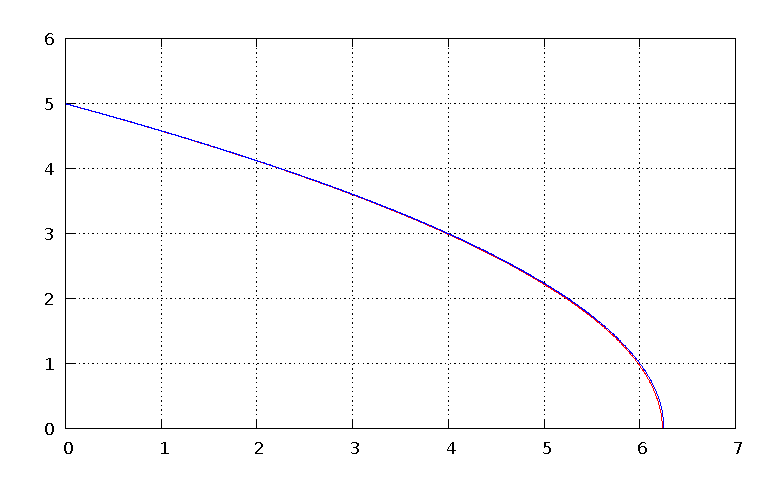
\includegraphics[width=.45\textwidth]
{figures/geometric_pdes/mcf_sphere_radius.ps}
\caption[Mean curvature flow shrinking sphere radius]{Average radius of a
sphere of initial radius $r_0=5$ subject to mean curvature flow. In blue the
analytical solution while in red the computed one.}
\label{fig:mcf_sphere_radius}
\end{figure}

\subsection{Equidistribution property}\label{subsec:sd_circle}
In order to show the equidistribution property of the scheme, we simulate the
evolution, under surface diffusion, of a circle of radius $r_0=0.5$ with a very
poor initial mesh quality. Indeed, the initial curve consists of a semi-circle
and a single additional node on the periphery of the circle for a total number
of mesh elements equal to $J_\Gamma=32$.

Figure~\ref{fig:sd_circle} shows the mesh evolution at time $t=0$, $t=0.05$,
$t=0.25$ and $t=10$ respectively with a constant time step equal to
$\tau=10^{-2}$. One can clearly see that although the true solution, which is a
circle, is reached very quickly, in the remaining time the vertices are
continually moved tangentially, which results in a further decrease in the ratio
\begin{equation}
\frac{\max_{\sigma\in \Gamma^m}\surfvol(\sigma)}
{\min_{\sigma\in\Gamma^m}\surfvol(\sigma)}\,,
\end{equation}
which approaches the optimal value 1. This mesh quality indicator is simply the
ratio between the maximum and minimum segment of the hypersurface.

\begin{figure}[htbp]
\centering
\subfloat[$t=0$]{\includegraphics[width=.45\textwidth]
{figures/geometric_pdes/sd_circle_0.ps}}
\subfloat[$t=0.05$]{\includegraphics[width=.45\textwidth]
{figures/geometric_pdes/sd_circle_005.ps}}\\
\subfloat[$t=0.25$]{\includegraphics[width=.45\textwidth]
{figures/geometric_pdes/sd_circle_025.ps}}
\subfloat[$t=10$]{\includegraphics[width=.45\textwidth]
{figures/geometric_pdes/sd_circle_10.ps}}
\caption[Surface diffusion equidistribution property]{Surface evolution of a
circle of initial radius $r_0=0.5$ subject to surface diffusion.}
\label{fig:sd_circle}
\end{figure}

In Figure~\ref{fig:sd_circle_tau} we see that the equidistribution velocity is
varying inversely with the size of $\tau$. For example, when $\tau=10^{-4}$,
the equidistribution is reached almost instantaneously.

\begin{figure}[htbp]
\centering
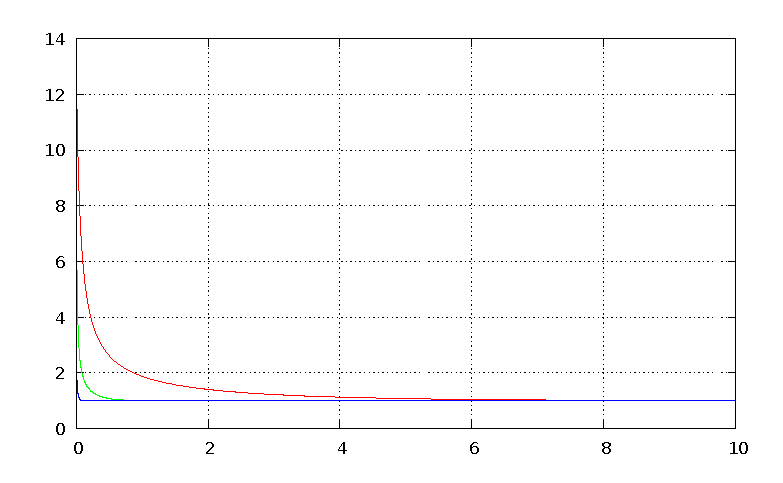
\includegraphics[width=.45\textwidth]
{figures/geometric_pdes/sd_circle_tau.ps}
\caption[\sloppy Surface diffusion equidistribution velocity]{Time evolution of
the ratio $\frac{\max_{\sigma\in \Gamma^m}\surfvol(\sigma)}
{\min_{\sigma\in\Gamma^m}\surfvol(\sigma)}$ for a circle of initial radius
${r_0=0.5}$ subject to surface diffusion. In red $\tau=10^{-2}$, in green
$\tau=10^{-3}$ and in blue $\tau=10^{-4}$.}
\label{fig:sd_circle_tau}
\end{figure}

\subsection{Surface diffusion with a cage as initial condition}
\label{subsec:sd_cage}
Our last simulation is inspired by the test in \cite[Fig.~15]{gflows3d}. We
investigate the evolution of a cage subject to surface diffusion. The
dimensions of the initial surface are $4 \times 4 \times 4$, with the region
enclosed by $\Gamma(0)$ given as the union of 12 cuboids of dimension $4 \times
1 \times 1$.

Figure~\ref{fig:sd_cage} shows the cage evolution at time $t=0$, $t=0.2$,
$t=0.4$ and $t=0.6$ respectively. The number of mesh elements is
$J_\Gamma=3816$ and the time step is constant and equal to $\tau=10^{-2}$.

\begin{figure}[htbp]
\centering
\subfloat[$t=0$]{\includegraphics[width=.45\textwidth]
{figures/geometric_pdes/sd_cage_0.ps}}
\subfloat[$t=0.2$]{\includegraphics[width=.45\textwidth]
{figures/geometric_pdes/sd_cage_02.ps}}\\
\subfloat[$t=0.4$]{\includegraphics[width=.45\textwidth]
{figures/geometric_pdes/sd_cage_04.ps}}
\subfloat[$t=0.6$]{\includegraphics[width=.45\textwidth]
{figures/geometric_pdes/sd_cage_06.ps}}
\caption[Surface diffusion cage]{Surface evolution of a cage $4 \times 4 \times
4$ subject to surface diffusion.}
\label{fig:sd_cage}
\end{figure}

At time $t=0.6$ a topological change is encountered when the six holes of the
surface are about to close to form a hollow ball.
Figure~\ref{fig:sd_cage_section} shows a section of this hallow ball. This
hallow ball is still topological equivalent with the cage, i.e. genus is 5.
Indeed we can see 6 very long and thin strands of elements, which connect the
inner ball with the outer ball.  A topological change breaks the front tracking
approach since the reference manifold $\Gamma^m$ is not topological compatible
with the unknown surface $\Gamma^{m+1}$. In practice, it is possible to apply
some heuristic algorithms for the detection of topological changes, such as the
merging of surfaces into one or the pinching-off of one surface from another,
which can lead to a modified surface mesh that can be handled again with the
parametric approach, see \cite{Sacconi}.

\begin{figure}[htbp]
\centering
\includegraphics[width=.45\textwidth]
{figures/geometric_pdes/sd_cage_06_section.ps}
\caption[Surface diffusion cage section]{Section at $t=0.6$ of a cage $4 \times
4 \times 4$ subject to surface diffusion.}
\label{fig:sd_cage_section}
\end{figure}

Finally, Figure~\ref{fig:sd_cage_energy} shows the evolution of the surface
energy (\ref{eq:surface_energy}) over time. As expected, see
(\ref{eq:area_decrease}), this energy is monotonically decreasing.

\begin{figure}[htbp]
\centering
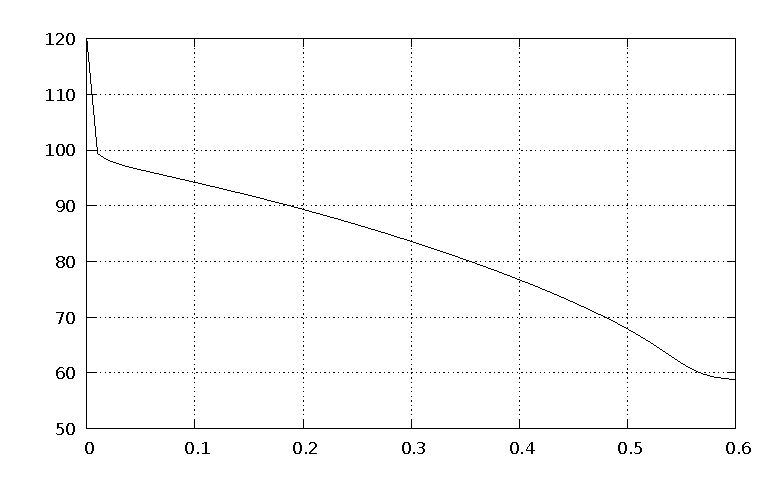
\includegraphics[width=.45\textwidth]
{figures/geometric_pdes/sd_cage_energy.ps}
\caption[Surface diffusion cage surface energy]{Surface energy evolution
$\surfvol(\Gamma^m)$ of a cage $4 \times 4 \times 4$ subject to surface
diffusion.}
\label{fig:sd_cage_energy}
\end{figure}

\chapter{\sc Two-Phase Stokes Flow}\label{ch:stokes}
We now propose a novel finite element approximation for incompressible
two-phase Stokes flow that naturally avoids spurious velocities. Our scheme uses
a fitted approach with piecewise linear parametric finite elements to describe
the moving discrete interface and employs standard velocity and pressure finite
element spaces in the bulk. This chapter is extensively based on a paper we
wrote, see \cite{stokesfitted}.

The chapter is organised as follows: in \S\ref{sec:stokes_model} we state the
mathematical model for the incompressible two-phase Stokes flow; in
\S\ref{sec:stokes_weak} we derive the weak formulation on which our finite
element approximation is going to be based; in \S\ref{sec:stokes_energy} we show
an energy bound and the volume conservation for the weak problem; in
\S\ref{sec:stokes_fem} we present our fitted finite element discretization; in
\S\ref{sec:stokes_fitted_unfitted} we outline the main differences between a
fitted and an unfitted approach; in \S\ref{sec:stokes_existence} we prove the
existence and uniqueness of the discrete approximation; in
\S\ref{sec:stokes_stability} we demonstrate that our scheme is unconditionally
stable; in \S\ref{sec:stokes_stationary_solution} show some proprieties of
stationary solutions which will be investigated in the numerical experiments; in
\S\ref{sec:stokes_semi_fem} we investigate the equidistribution property and the
volume conservation of a semidiscrete variant of the scheme; in
\S\ref{sec:stokes_algebraic_system} we describe the arising linear systems; in
\S\ref{sec:stokes_solution_method} we explain the Schur complement approach used
to solve the algebraic system and the preconditioners adopted; in
\S\ref{sec:stokes_smoothing} we discuss the mesh generation process together
with the smoothing and remeshing procedures used to preserve the mesh quality;
in \S\ref{sec:stokes_results} we finally present several numerical simulations
in 2d and 3d.

\section{Mathematical model}\label{sec:stokes_model}
We consider two-phase Stokes flow in a given domain $\Omega\subset\R^d$, where
$d=2$ or $d=3$. As already described in \S\ref{sec:free_boundary_flows},
the domain $\Omega$ contains two different immiscible, incompressible, viscous
fluids (liquid-liquid or liquid-gas) which for all $t\in[0,T]$ occupy time
dependent regions $\Omega_+(t)$ and
$\Omega_-(t):=\Omega\setminus\overline{\Omega}_+(t)$ and which are separated by
an interface $(\Gamma(t))_{t\in[0,T]}$, $\Gamma(t)\subset\Omega$. In this
thesis, we always treat interfaces formed by closed hypersurfaces, as
illustrated in Figure~\ref{fig:two_phase_sketch} for dimension $d=2$.

The interface $\Gamma(t)$ is described with the same technique used in the
approximation of mean curvature flow and surface diffusion, see
Chapter~\ref{ch:geometric_pdes}. More precisely, we use a front tracking
approach, see \S\ref{sec:front_tracking_approach}, which parametrize the
unknown interface $\Gamma(t)$ as $\vec x(\cdot,t):\Upsilon\to\R^d$ where
$\Upsilon\subset\R^d$ is a given reference manifold such that $\Gamma(t) = \vec
x(\Upsilon,t)$. We always require that the evolving hypersurface is sufficiently
smooth and without boundary. Therefore, the velocity $\V$ of $\Gamma(t)$ is
defined by the equation (\ref{eq:V}) which we report here for the benefit of
the reader
\begin{equation*}
\V(\vec z, t) := \vec x_t(\vec q, t) \quad
\forall\ \vec z = \vec x(\vec q,t) \in \Gamma(t)\,,
\end{equation*}
where $\V \,.\,\vec \nu$ is the normal velocity of the evolving hypersurface
$\Gamma(t)$ and $\vec\nu(t)$ is the unit normal on $\Gamma(t)$ pointing into
$\Omega_+(t)$.

\sloppy The fluid dynamics in the bulk domain $\Omega$ is governed by the
two-phase Stokes model (\ref{eq:momentum_bis}--b) which describes the velocity
$\vec u$ and pressure $p$ fields of the fluid. The velocity and stress tensor,
see (\ref{eq:stress_tensor}), needs to be coupled across the free surface
$\Gamma(t)$ and therefore we impose the interface conditions
(\ref{eq:interface_jump_velocity}), (\ref{eq:interface_jump_stress}) and
(\ref{eq:interface_velocity}). Let $\partial\Omega$ be
partitioned as $\partial\Omega=\partial_1\Omega \cup \partial_2\Omega$ with
${\partial_1\Omega \cap \partial_2\Omega = \emptyset}$. We impose, on
$\partial_1 \Omega$, the Dirichlet condition $\vec u = \vec g$ and, on
$\partial_2 \Omega$, the free-slip condition $\vec u \,.\,\unitn = 0$,
with $\unitn$ denoting the outer unit normal of $\partial \Omega$. Finally, to
close the system, we prescribe the initial data $\Gamma(0) = \Gamma_0$.
Therefore the total system can be rewritten as follows:
\begin{subequations}
\begin{alignat}{2}
-2 \mu\,\nabla\,.\,\mat D(\vec u)+ \nabla\,p & = \vec f
\quad &&\mbox{in } \Omega_\pm(t)\,, \label{eq:stokes_full_momentum} \\
\nabla\,.\,\vec u & = 0 \quad &&\mbox{in } \Omega_\pm(t)\,,
\label{eq:stokes_full_mass} \\
\vec u & = \vec g \quad &&\mbox{on } \partial_1\Omega\,,
\label{eq:stokes_full_dirichlet}\\
\vec u \,.\,\unitn & = 0 \quad &&\mbox{on } \partial_2\Omega\,,
\label{eq:stokes_full_freeslip}\\
[\vec u]_-^+ & = \vec 0 \quad &&\mbox{on } \Gamma(t)\,,
\label{eq:stokes_full_jump_velocity} \\
[2\mu \,\mat D(\vec u)\,.\,\vec\nu - p\,\vec \nu]_-^+
& = -\gamma\,\varkappa\,\vec\nu
\quad &&\mbox{on } \Gamma(t)\,, \label{eq:stokes_full_jump_stress} \\
(\V-\vec u)\,.\,\vec \nu & = 0
\quad &&\mbox{on } \Gamma(t)\,,\label{eq:stokes_full_velocity}  \\
\Gamma(0) & = \Gamma_0 \,,\label{eq:stokes_full_initial_interface}
\end{alignat}
\end{subequations}
where $\mu(t) = \mu_+\,\charfcn{\Omega_+(t)} + \mu_-\,\charfcn{\Omega_-(t)}$,
with $\mu_\pm \in \R_{>0}$, denotes the dynamic viscosities in the two phases,
$\mat D(\vec u):=\frac12\, (\nabla\vec u+(\nabla\vec u)^T)$
is the rate-of-deformation tensor, $\vec f$ is a possible forcing term,
$\gamma>0$ is the surface tension coefficient and $\varkappa$ denotes the
mean curvature of $\Gamma(t)$. See Chapter~\ref{ch:introduction} for more
details.

\section{Weak formulation}\label{sec:stokes_weak}
In order to obtain a weak formulation, we define the function spaces, for a
given $\vec b \in [H^1_0(\Omega)]^d$,
\begin{align*}
\uspace b &:= \{\vec \phi\in[H^1_0(\Omega)]^d:\vec \phi =\vec
g\quad \mbox{on }\partial_1\Omega\}\,,\\
\pspace &:= L^2(\Omega)\,,\\
\pnormspace &:= \{\eta\in\pspace : \int_\Omega\eta\dL{d}=0 \}\,,
\end{align*}
and let, as usual, $(\cdot,\cdot)$ and $\langle \cdot, \cdot
\rangle_{\Gamma(t)}$ denote the $L^2$--inner products on $\Omega$ and
$\Gamma(t)$, respectively. In addition, we let $\vol$ and $\surfvol$ denote the
Lebesgue measure in $\R^d$ and the $(d-1)$-dimensional Hausdorff measure,
respectively.

We also need a weak form of the differential geometry identity
(\ref{eq:LBop}) which can be obtained by multiplying (\ref{eq:LBop}) with a
test function and performing integration by parts yielding to
$$
\left\langle \varkappa\,\vec\nu, \vec\eta \right\rangle_{\Gamma(t)}
+ \left\langle \nabs\,\vec \id, \nabs\,\vec \eta \right\rangle_{\Gamma(t)}
= 0  \quad \forall\ \vec\eta \in [H^1(\Gamma(t))]^d\,.
$$
Moreover, on noting (\ref{eq:stress_tensor}) and
(\ref{eq:interface_jump_stress}), we have that
\begin{align*}
\int_{\Omega_+(t)\cup\Omega_-(t)} (\nabla\,.\,\mat\sigma)\,.\, \vec \xi \dL{d}
& = - \left(\mat\sigma, \nabla\,\vec \xi\right)
- \left\langle [\mat\sigma\,\vec\nu]_-^+ , \vec \xi
  \right\rangle_{\Gamma(t)} \nonumber \\
& = \left( p , \nabla\,.\,\vec \xi\right)
-2 \left(\mu\,\mat D(\vec u) , \mat D(\vec \xi) \right)
+ \gamma \left\langle \varkappa\,\vec \nu , \vec \xi  \right\rangle_{\Gamma(t)}
\end{align*}
for all $\vec \xi \in \uspace 0$. Hence a possible weak formulation of
(\ref{eq:stokes_full_momentum}--h) is given as follows.
\sloppy Given $\Gamma(0) = \Gamma_0$, for almost all $t\in(0,T)$ find
$\Gamma(t)$ and ${(\vec u, p, \varkappa) \in \uspace g \times \pnormspace
\times H^1(\Gamma(t))}$ such that
\begin{subequations}
\begin{align}
& 2\left(\mu\,\mat D(\vec u), \mat D(\vec \xi)\right)
- \left(p, \nabla\,.\,\vec \xi\right)
- \gamma\,\left\langle \varkappa\,\vec\nu, \vec\xi\right\rangle_{\Gamma(t)}
= \left(\vec f, \vec \xi\right)\quad \forall\ \vec\xi \in \uspace 0 \,,
\label{eq:stokes_weaka}\\
& \left(\nabla\,.\,\vec u, \varphi\right) = 0
\quad \forall\ \varphi \in \pnormspace\,, \label{eq:stokes_weakb} \\
&  \left\langle \V
- \vec u, \chi\,\vec\nu \right\rangle_{\Gamma(t)} = 0
\quad \forall\ \chi \in H^1(\Gamma(t))\,, \label{eq:stokes_weakc} \\
& \left\langle \varkappa\,\vec\nu, \vec\eta \right\rangle_{\Gamma(t)}
+ \left\langle \nabs\,\vec \id, \nabs\,\vec \eta \right\rangle_{\Gamma(t)}
= 0  \quad \forall\ \vec\eta \in [H^1(\Gamma(t))]^d\,\label{eq:stokes_weakd}
\end{align}
\end{subequations}
holds for almost all times $t \in (0,T]$. Here we have observed that if
$p \in \pspace$ is part of a solution to (\ref{eq:stokes_full_momentum}--h),
then so is $p + c$ for an arbitrary $c\in \R$.

We finally observe that an alternative weak formulation can be obtained
using directly the vector quantity $\vec\varkappa:=\varkappa\,\vec\nu$
in the identity (\ref{eq:LBop}), see in \cite{Dziuk91,Bansch01,GanesanMT07}.
Instead, consistently with Chapter~\ref{ch:geometric_pdes}, we follow the
approach introduced in \cite{triplej} for $d=2$ and in \cite{gflows3d} for
$d=3$ which treats the mean curvature as a scalar and we treat it
separately from the normal $\vec\nu$, because this approach leads to good mesh
properties and to smaller algebraic systems.

\section{Energy bound and volume conservation}\label{sec:stokes_energy}
It is straightforward to show an a priori energy bound, in the absence of
external forces, and a volume conservation property for the system
(\ref{eq:stokes_weaka}--d). For the former, we use (\ref{eq:length_variation})
and we obtain
\begin{equation}\label{eq:dtarea}
\ddt\,\surfvol(\Gamma(t)) = -
\left\langle \varkappa,\V\,.\,\vec\nu\right\rangle_{\Gamma(t)}.
\end{equation}
Hence, in the case $\vec g=\vec 0$, on choosing $\vec\xi = \vec u$ in
(\ref{eq:stokes_weaka}), and noting
(\ref{eq:stokes_weakb},c), we obtain that
\begin{align}
\gamma\, \ddt\,\surfvol(\Gamma(t)) = -
\gamma\,\left\langle \varkappa\,\vec\nu, \vec u\right\rangle_{\Gamma(t)}
=  - 2\left(\mu\,\mat D(\vec u), \mat D(\vec u)\right) +
\left(\vec f, \vec u\right) \,,
\label{eq:ap1}
\end{align}
and so in the absence of outer forces, the interfacial energy is monotonically
decreasing.

In order to show the volume conservation property, we use
(\ref{eq:volume_variation}) to have that
\begin{align}
\ddt \vol(\Omega_-(t)) & = \left\langle \V, \vec\nu
\right\rangle_{\Gamma(t)}\,.
\end{align}
Hence it follows immediately from the incompressibility condition
(\ref{eq:stokes_weakb}) and (\ref{eq:stokes_weakc}) that
\begin{align}
\ddt \vol(\Omega_-(t)) & = \left\langle \vec u , \vec\nu
\right\rangle_{\Gamma(t)}
 = \int_{\Omega_-(t)} \nabla\,.\,\vec u \dL{d} =0\,. \label{eq:conserved}
\end{align}
It will be our aim to introduce a fitted finite element approximation for
two-phase Stokes flow that satisfies discrete analogous of
(\ref{eq:ap1}) and (\ref{eq:conserved}).

\section{Finite element approximation}\label{sec:stokes_fem}
We consider the partitioning  $0= t_0 < t_1 < \ldots < t_{M-1} < t_M = T$ of
$[0,T]$ into possibly variable time steps $\tau_m := t_{m+1}-t_m$, $m=0
,\ldots, M-1$. Moreover, let ${\cal T}^m$, $\forall m\ge 0$, be a regular
partitioning of the domain $\Omega$ into disjoint open simplices
$\sigmaO^m_j$, $j = 1 ,\ldots, J^m_\Omega$. On ${\cal T}^m$ we define the
finite element spaces
\begin{equation*}
S^m_k := \{\chi \in C(\overline{\Omega}) : \chi\!\mid_{\sigmaO^m}
\in \mathcal{P}_k(\sigmaO^m) \ \forall\ \sigmaO^m \in {\cal T}^m\}\,,
\quad k \in \mathbb{N}\,,
\end{equation*}
where $\mathcal{P}_k(\sigmaO^m)$ denotes the space of polynomials of degree $k$
on $\sigmaO^m$. Moreover, $S^m_0$ is the space of piecewise constant functions
on ${\cal T}^m$. For later use, we also define $\vec I^m_k$ to be the standard
interpolation operator onto $[S^m_k]^d$.

Let $\uspacedisc{g}{m}\subset\uspacesimple(\vec I_k^m\vec g)$ and
$\pspace^m\subset\pspace$ be the finite element spaces we use for the
approximation of velocity and pressure, and let $\pnormspace^m:= \pspace^m \cap
\pnormspace$. The spaces $(\uspacedisc{0}{m},\pspace^m)$ satisfy the LBB
inf-sup condition if there exists a constant $C_0 \in \R_{>0}$, independent of
$\mathcal{T}^m$, such that
\begin{equation} \label{eq:LBB}
\inf_{\varphi \in \pnormspace^m} \sup_{\vec \xi \in \uspacedisc{0}{m}}
\frac{( \varphi, \nabla \,.\,\vec \xi)} {\|\varphi\|_0\,\|\vec \xi\|_1}
\geq C_0 > 0\,,
\end{equation}
see \cite[p.~114]{GiraultR86}. Here $\|\cdot\|_0 := (\cdot,\cdot)^\frac12$ and
$\|\cdot\|_1 := \|\cdot\|_0 + \|\nabla\,\cdot\|_0$ denote the $L^2$--norm and
the $H^1$--norm on $\Omega$, respectively. Throughout this thesis, if not
otherwise stated, we will assume that $\charfcn{\Omega^m_-}\in\pspace^m$. Then,
for $d=2$, possible pairs $(\uspacedisc{0}{m},\pspace^m)$ that satisfy
(\ref{eq:LBB}) are P2--P0 and P2--(P1+P0), i.e. we set
$\uspacedisc{0}{m}=[S^m_2]^d\cap\uspace{0}$ and either $\pspace^m = S^m_0$ or
$S^m_1+S^m_0$. We note that the choice P2--(P1+P0) requires the weak constraint
that all simplices have a vertex in $\Omega$, see \cite{BoffiCGG12}. For $d=3$,
pairs of spaces that satisfy $\charfcn{\Omega^m_-}\in\pspace^m$ and
(\ref{eq:LBB}) are the P3--(P2+P0) element, see \cite{BoffiCGG12}, or stabilized
spaces such as P1$^{\mbox{face bubble}}$--P0, see
\cite[Remark~8.7.1]{BoffiBF13}, which is also called the SMALL element. With a
view towards our numerical simulations, we also introduce the pairs P2--\pdg
where the space \pdg is a space of polynomial order 1 defined in the two
subdomains $\Omega_-^m$ and $\Omega_+^m$. This space is equivalent to a P1 space
which is continuous everywhere except across the interface $\Gamma^m$. With this
choice of space, the discrete scheme fall in the category of XFEM, extended
FEM, since the pressure space is enriched adding additional degree of freedoms
for the nodes on the interface in order to capture the discontinuity of the
pressure.

In this thesis we consider a fitted finite element approximation for the
evolution of the interface $\Gamma(t)$. Let $\Gamma^m\subset\R^d$ be a
$(d-1)$-dimensional polyhedral surface approximating the closed surface
$\Gamma(t_m)$, $m=0 ,\ldots, M$. Let $\Omega^m_+$ denote the exterior of
$\Gamma^m$ and let $\Omega^m_-$ be the interior of $\Gamma^m$, where we assume
that $\Gamma^m$ has no self-intersections. Then
$\Omega = \Omega_-^m \cup \Gamma^m \cup \Omega_+^m$, and the fitted nature of
our method implies that
\begin{equation} \label{eq:fittedO}
\overline{\Omega^m_+} = \bigcup_{o \in \mathcal{T}^m_+} \overline{o}
\quad\text{and}\quad
\overline{\Omega^m_-} = \bigcup_{o \in \mathcal{T}^m_-} \overline{o} \,,
\end{equation}
where $\mathcal{T}^m = \mathcal{T}^m_+ \cup \mathcal{T}^m_-$ and
$\mathcal{T}^m_+ \cap \mathcal{T}^m_- = \emptyset$.
Let $\vec \nu^m$ denote the piecewise constant unit normal to $\Gamma^m$
such that $\vec\nu^m$ points into $\Omega^m_+$.

In order to define the parametric finite element spaces on $\Gamma^m$, we
assume that $\Gamma^m=\bigcup_{j=1}^{J_\Gamma} \overline{\sigma^m_j}$, where
$\{\sigma^m_j\}_{j=1}^{J_\Gamma}$ is a family of mutually disjoint open
$(d-1)$-simplices with vertices $\{\vec q^m_k\}_{k=1}^{K_\Gamma}$. Following
the notation in \cite{spurious}, see also \cite{gflows3d}, we define
$\Vh := \{\vec\chi \in [C(\Gamma^m)]^d:\vec\chi\!\mid_{\sigma^m_j}
\in \mathcal{P}_1(\sigma^m_j), j=1,\ldots, J_\Gamma\} =: [\Wh]^d$,
where $\Wh \subset H^1(\Gamma^m)$ is the space of scalar continuous
piecewise linear functions on $\Gamma^m$, with $\{\chi^m_k\}_{k=1}^{K_\Gamma}$
denoting the standard basis of $\Wh$.

Moreover we define $\pi^m: C(\Gamma^m)\to \Wh$ the standard interpolation
operator at the nodes $\{\vec q_k^m\}_{k=1}^{K_\Gamma}$, and similarly
$\vec\pi^m: [C(\Gamma^m)]^d\to \Vh$. Throughout this thesis, we parametrize
the new surface $\Gamma^{m+1}$ over $\Gamma^m$ using a parametrization
$\vec X^{m+1} \in \Vh$, so that $\Gamma^{m+1} = \vec X^{m+1}(\Gamma^m)$.

In order to have the desired tangential motion of vertices on $\Gamma^m$
that leads to good interface mesh properties, for the interface terms we again
use the mass lumped inner product $\langle\cdot,\cdot\rangle_{\Gamma^m}^h$, see
(\ref{eq:masslump}). Finally, let $\langle\cdot,\cdot\rangle_{\Gamma^m}$ denote
the standard $L^2$--inner product on $\Gamma^m$.

\sloppy Then our finite element approximation, which is based on the variational
formulation (\ref{eq:stokes_weaka}--d), assumes the following formulation. Let
$\Gamma^0$ be an approximation to the initial interface $\Gamma(0)$. For
$m=0,\ldots, M-1$, find ${(\vec U^{m+1}, P^{m+1}, \vec X^{m+1}, \kappa^{m+1})
\in \uspacedisc{g}{m}\times \pnormspace^m \times \Vh \times \Wh}$ such that
\begin{subequations}
\begin{align}
& 2\left(\mu^m\,\mat D(\vec U^{m+1}), \mat D(\vec \xi) \right)
- \left(P^{m+1}, \nabla\,.\,\vec \xi\right) \nonumber \\
& - \gamma\,\left\langle \kappa^{m+1}\,\vec\nu^m,\vec\xi\right\rangle_{\Gamma^m}
= \left(\vec f^{m+1},\vec \xi\right) \quad \forall\ \vec\xi \in
\uspacedisc{0}{m}\,, \label{eq:HGa}\\
& \left(\nabla\,.\,\vec U^{m+1}, \varphi\right)  = 0
\quad \forall\ \varphi \in \pnormspace^m\,,\label{eq:HGb} \\
&  \left\langle \frac{\vec X^{m+1} - \vec\id}{\tau_m} ,\chi\,\vec\nu^m
\right\rangle_{\Gamma^m}^h - \left\langle \vec U^{m+1}, \chi\,\vec\nu^m
\right\rangle_{\Gamma^m}  = 0 \quad \forall\ \chi \in \Wh\,, \label{eq:HGc} \\
& \left\langle \kappa^{m+1}\,\vec\nu^m, \vec\eta \right\rangle_{\Gamma^m}^h
+ \left\langle \nabs\,\vec X^{m+1}, \nabs\,\vec \eta \right\rangle_{\Gamma^m} =
0 \quad \forall\ \vec\eta \in \Vh \label{eq:HGd}
\end{align}
\end{subequations}
and set $\Gamma^{m+1} = \vec X^{m+1}(\Gamma^m)$. Here we have defined
$\vec f^{m+1}(\cdot) := \vec I^m_2\,\vec f(\cdot,t_{m+1})$ and
\begin{equation}
\mu^m =\mu_+\,\charfcn{\Omega^m_+} + \mu_-\,\charfcn{\Omega^m_-}\in S^m_0\,.
\end{equation}
We observe that (\ref{eq:HGa}--d) is a linear scheme in that it leads to a
coupled linear system of equations for the unknowns
$(\vec U^{m+1}, P^{m+1}, \vec X^{m+1}, \kappa^{m+1})$ at each time level.
We also note that the scheme (\ref{eq:HGa}--d), in the context of an
unfitted finite element approximation, has been considered in \cite{spurious}.
In particular, most of the theoretical results presented in the following
are a direct consequence of the results in \cite{spurious}.

\section{Fitted and unfitted approach}\label{sec:stokes_fitted_unfitted}
The key difference between \cite{spurious} and our approach is that the former
uses an unfitted approach while the latter adopts a fitted one. In
Figure~\ref{fig:fitted_unfitted}, from \cite[Fig.~1]{spurious}, is shown an
example of fitted and unfitted interface meshes for a circular interface.
\begin{figure}[htbp]
\centering
\subfloat[Fitted mesh]{
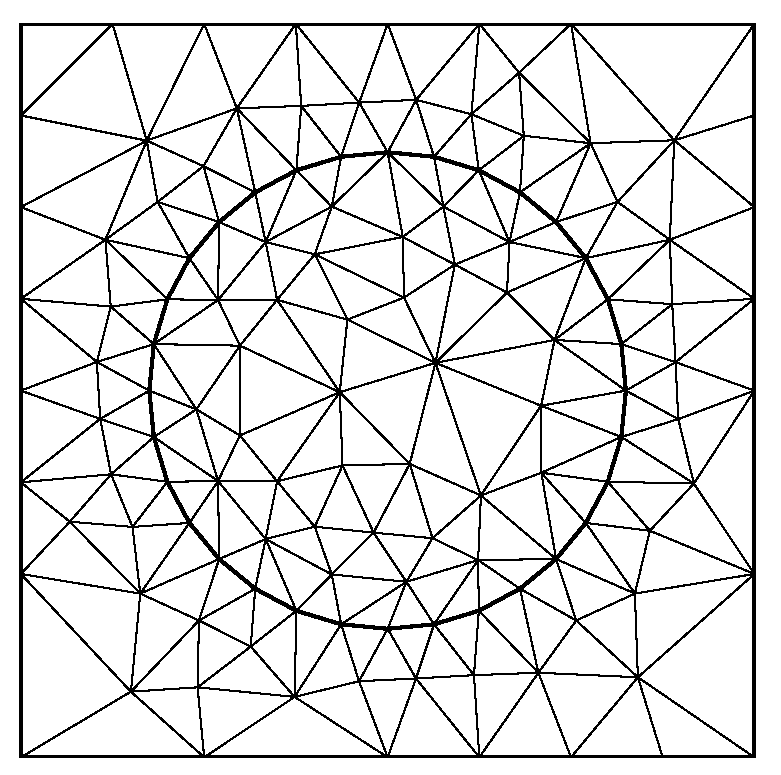
\includegraphics[width=.45\textwidth]
{figures/stokes/fitted_mesh.ps}}
\subfloat[Unfitted mesh]{
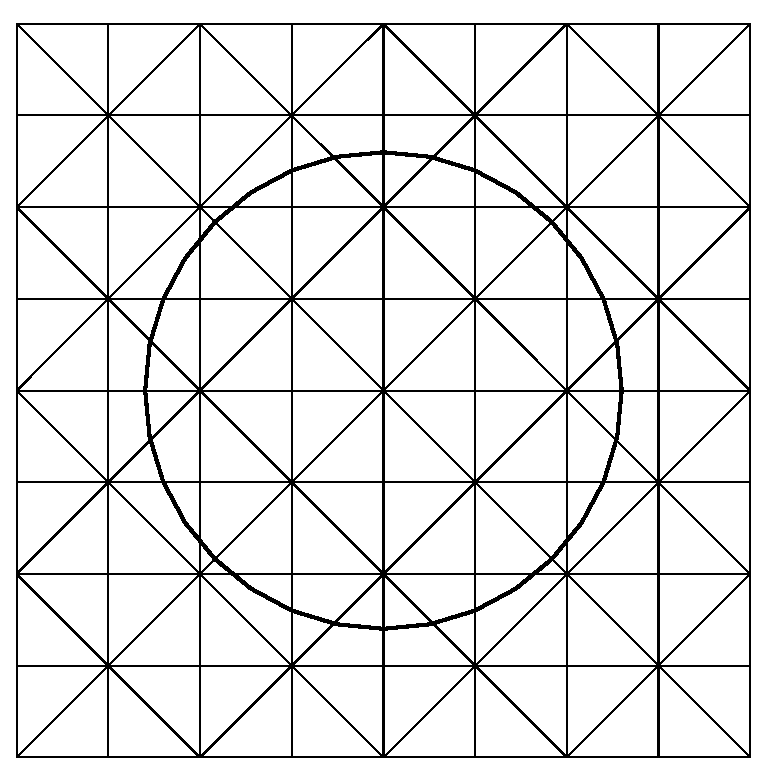
\includegraphics[width=.45\textwidth]
{figures/stokes/unfitted_mesh.ps}}
\caption[Fitted and unfitted meshes]
{Fitted and unfitted meshes for a circular interface.}
\label{fig:fitted_unfitted}
\end{figure}
In the fitted approach, the interface mesh is made up of edges, in 2d, or faces,
in 3d, of elements belonging to the bulk mesh. This means that there is a strong
coupling between the bulk mesh and interface mesh. This is a very intuitive
approach to treat the problem. Discontinuity jumps in the material properties
and in the pressure are captured naturally. In particular, we do not need to
employ an XFEM-type extension of standard bulk pressure spaces. Moreover, there
is no need to transport quantities from the interface to the bulk, or vice
versa. On the other hand, it is not possible to locally refine the bulk mesh
close to the interface without modifying the number of elements of the
interface. Also, every interface deformation corresponds to a bulk deformation,
which means that smoothing and remeshing techniques need to be employed in
order to preserve the bulk mesh quality.

Instead, in the unfitted approach, the interface mesh is completely independent
from the bulk mesh. In particular, there exist bulk elements which are cut by
the interface elements. For this reason there is no need to remesh or deform
the bulk mesh in order to preserve the correspondence with the interface.
Moreover, standard strategies for refinement and coarsening can be employed for
the bulk mesh. Since the bulk mesh is immutable, its quality is preserved
without the need of smoothing techniques. The downside of this approach is that
the quantities computed on the bulk mesh, such as velocity and pressure, need
to be interpolated in order to have their values on the interface. This also
requires to find the intersections between the interface mesh and the bulk mesh
at every time step. Finally, it is necessary to use some XFEM-type extension in
order to capture discontinuity of quantities of interest across the interface.

\section{Existence and uniqueness of a discrete solution}
\label{sec:stokes_existence}
\begin{theorem} \label{thm:ex}
Let $m \in \{0,\ldots,M-1\}$ and let $(\uspacedisc{0}{m},\pspace^m)$ satisfy
the LBB condition (\ref{eq:LBB}). Then there exists a unique solution
$(\vec U^{m+1}, P^{m+1}, \vec X^{m+1}, \kappa^{m+1})
\in \uspacedisc{g}{m}\times \pnormspace^m \times \Vh \times \Wh$ to
(\ref{eq:HGa}--d).
\end{theorem}
\begin{proof}
\sloppy As the system (\ref{eq:HGa}--d) is linear, existence follows from
uniqueness. In order to establish the latter, we consider the system: Find
${(\vec U, P, \vec X, \kappa) \in \uspacedisc{0}{m}\times\pnormspace^m \times
\Vh \times \Wh}$ such that
\begin{subequations}
\begin{align}
& 2\left(\mu^m\,\mat D(\vec U), \mat D(\vec \xi) \right)
- \left(P, \nabla\,.\,\vec \xi\right) - \gamma\,\left\langle \kappa\,\vec\nu^m,
\vec\xi\right\rangle_{\Gamma^m} = 0 \quad \forall\ \vec\xi \in
\uspacedisc{0}{m} \,,
\label{eq:proofa}\\
& \left(\nabla\,.\,\vec U, \varphi\right)  = 0 \quad
\forall\ \varphi \in \pnormspace^m\,, \label{eq:proofb} \\
& \left\langle \vec X, \chi\,\vec\nu^m \right\rangle_{\Gamma^m}^h -
\tau_m \left\langle \vec U, \chi\,\vec\nu^m \right\rangle_{\Gamma^m} = 0
\quad\forall\ \chi \in \Wh\,,\label{eq:proofc} \\
& \left\langle \kappa\,\vec\nu^m, \vec\eta \right\rangle_{\Gamma^m}^h
+ \left\langle \nabs\,\vec X, \nabs\,\vec \eta \right\rangle_{\Gamma^m}
= 0  \quad\forall\ \vec\eta \in \Vh\,. \label{eq:proofd}
\end{align}
\end{subequations}
Choosing $\vec\xi=\vec U$ in (\ref{eq:proofa}), $\varphi =  P$ in
(\ref{eq:proofb}), $\chi = \gamma\,\kappa$ in (\ref{eq:proofc}) and
$\vec\eta=\gamma\,\vec X$ in (\ref{eq:proofd}) yields that
\begin{equation}
2\,\tau_m\left(\mu^m\,\mat D(\vec U), \mat D(\vec U) \right)
+ \gamma\,\left\langle \nabs\,\vec X, \nabs\,\vec X \right\rangle_{\Gamma^m}
=0\,. \label{eq:proof2}
\end{equation}
It immediately follows from (\ref{eq:proof2}) and a Korn's inequality that
$\vec U = \vec 0$. In addition, it holds that $\vec X$ is equal to a constant
on $\Gamma^m$, which satisfies, on recalling (\ref{eq:proofc}) and $\vec U =
\vec 0$, that
\begin{equation} \label{eq:Xconst}
\left\langle \vec X, \chi\,\vec\nu^m \right\rangle_{\Gamma^m}^h = 0
\quad\forall\ \chi \in \Wh\,.
\end{equation}
It was shown in \cite[Proof of Theorem~2.1]{gflows3d} that if $\Gamma^m$
has no self-intersections, then (\ref{eq:Xconst}) immediately yields that $\vec
X = \vec 0$. As $\Gamma^m = \partial\Omega^m_-$ is the boundary of an open
domain, we always assume that it does not self-intersect, and
hence we obtain that $\vec X = \vec 0$. This means that (\ref{eq:proofd})
reduces to
\begin{equation} \label{eq:kappaproof}
\left\langle \kappa\,\vec\nu^m, \vec\eta \right\rangle_{\Gamma^m}^h = 0
\quad\forall\ \vec\eta \in \Vh\,.
\end{equation}
Let $\vec\omega^m \in \Vh$ be the mass-lumped $L^2$--projection of $\vec\nu^m$
onto $\Vh$, i.e. $\left\langle \vec\omega^m, \vec\varphi
\right\rangle_{\Gamma^m}^h = \left\langle \vec\nu^m,
\vec\varphi \right\rangle_{\Gamma^m}^h = \left\langle \vec\nu^m,
\vec\varphi \right\rangle_{\Gamma^m}$ for all $\vec\varphi\in\Vh$. It is easy
to see that $\vec\omega^m (\vec q^m_k) \not= \vec 0$ for
all $k=1,\ldots,K_\Gamma$, because $\Gamma^m$ does not self-intersect.
Then it follows from choosing $\vec\eta = \vec\omega^m$ in (\ref{eq:kappaproof})
that
\begin{align*}
0 = \left\langle \kappa\,\vec\nu^m, \vec\omega^m \right\rangle_{\Gamma^m}^h
= \left\langle \vec\nu^m, \vec\pi^m[\kappa\,\vec\omega^m]
\right\rangle_{\Gamma^m}
= \left\langle \vec\omega^m,
\vec\pi^m[\kappa\,\vec\omega^m] \right\rangle_{\Gamma^m}^h
= \left\langle \kappa, |\vec\omega^m|^2 \right\rangle_{\Gamma^m}^h ,
\end{align*}
and so $\kappa = 0 \in \Wh$. Finally, it follows from (\ref{eq:proofa}) with
$\vec U = \vec 0$ and $\kappa = 0$, on recalling (\ref{eq:LBB}), that $P = 0$.
Hence there exists a unique solution $(\vec U^{m+1}, P^{m+1}, \vec X^{m+1},$
$\kappa^{m+1}) \in \uspacedisc{g}{m}\times \pnormspace^m \times \Vh \times \Wh$
to
(\ref{eq:HGa}--d).
\end{proof}

We note that if $(\uspacedisc{0}{m},\pspace^m)$ does not satisfy the LBB
condition
(\ref{eq:LBB}), then existence and uniqueness of the solution
$(\vec U^{m+1},\vec X^{m+1},\kappa^{m+1})$ to a reduced system, where the
pressure $P^{m+1}$ is eliminated, can be shown. See \cite[Theorem~1]{spurious}
for more details.

\section{Stability}\label{sec:stokes_stability}
We now demonstrate that the scheme (\ref{eq:HGa}--d) satisfies an energy
estimate, which corresponds to the bound (\ref{eq:ap1}) in the continuous case.
In particular, we obtain an unconditional stability result for our scheme.

\begin{theorem} \label{thm:stabstab}
\sloppy Let $\vec g=\vec 0$. Moreover let $m \in \{0,\ldots,M-1\}$ and let
${(\vec U^{m+1},P^{m+1},\vec X^{m+1}, \kappa^{m+1}) \in \uspacedisc{0}{m}\times
\pnormspace^m \times \Vh \times \Wh}$ be a solution to (\ref{eq:HGa}--d). Then
\begin{equation}\label{eq:stab}
\gamma\, \surfvol(\Gamma^{m+1})
+ 2\,\tau_m\left(\mu^m\,\mat D(\vec U^{m+1}), \mat D(\vec U^{m+1}) \right) \leq
\gamma\,\surfvol(\Gamma^m) + \tau_m\left( \vec f^{m+1}, \vec U^{m+1}
\right).
\end{equation}
In addition, let $\{t_k\}_{k=0}^M$ be an arbitrary partitioning of $[0,T]$.

Then it holds that
\begin{equation}\label{eq:stabstab}
\gamma\,\surfvol(\Gamma^{m+1})
+ 2 \sum_{k=0}^m  \tau_k\left(\mu^k\,\mat D(\vec U^{k+1}), \mat D(\vec U^{k+1})
\right)\leq \gamma\,\surfvol(\Gamma^0) + \sum_{k=0}^m \tau_k\left(\vec
f^{k+1}, \vec U^{k+1} \right)
\end{equation}
for $m=0,\ldots, M-1$.
\end{theorem}
\begin{proof}
The desired results follow from choosing $\vec\xi = \vec U^{m+1} \in
\uspacedisc{0}{m}$ in (\ref{eq:HGa}), $\varphi = P^{m+1} \in \pnormspace^m$ in
(\ref{eq:HGb}), $\chi = \gamma\,\kappa^{m+1}$ in (\ref{eq:HGc}) and
$\vec\eta=\gamma\,({\vec X^{m+1}-\vec\id\!\mid_{\Gamma^m}})$ in
(\ref{eq:HGd}). See \cite[Proof of Theorem~2]{spurious} for more details.
\end{proof}

\section{Discrete stationary solutions}\label{sec:stokes_stationary_solution}
If the solution $(\vec U^{m+1},P^{m+1},\vec X^{m+1}, \kappa^{m+1})$ to
(\ref{eq:HGa}--d) is such that the interface has not moved,
$\Gamma^{m+1} = \Gamma^m$, then it holds that
\begin{equation}\label{eq:conformal}
\exists\ \zeta \in \Wh \ : \quad \left\langle \zeta\,\vec\nu^m, \vec\eta
\right\rangle_{\Gamma^m}^h + \left\langle \nabs\,\vec \id, \nabs\,\vec \eta
\right\rangle_{\Gamma^m} = 0 \quad \forall\ \vec\eta \in \Vh \,.
\end{equation}
We recall from \cite[Remark~2.4]{triplej} that (\ref{eq:conformal}) in the
case $d=2$ implies that $\Gamma^m$ is equidistributed, with the possible
exception of
elements $\sigma^m_j$ that are locally parallel to each other; see also
\cite[Theorem~2.2]{fdfi}.
Moreover, we recall from \cite[\S4.1]{gflows3d}
that surfaces $\Gamma^m \subset \R^3$
that satisfy (\ref{eq:conformal}) are called conformal polyhedral surfaces.

Next we consider discrete stationary states when no outer forces act, i.e. when
$\vec f = \vec 0$. Here, independently of the choice of $\mu_\pm$, no spurious
velocities appear for discrete stationary solutions. Indeed,
Theorem~\ref{thm:stabstab} has an immediate consequence.
\begin{theorem}\label{thm:stat1}
Let $\vec g=\vec 0$. Let $(\vec U^{m+1},P^{m+1},\vec X^{m+1}, \kappa^{m+1})
\in \uspacedisc{0}{m}\times
\pnormspace^m \times \Vh \times \Wh$ be a solution to  (\ref{eq:HGa}--d) with
$\vec f^{m+1} = \vec 0$. If $\vec X^{m+1} = \vec X^m$, then $\vec U^{m+1} = \vec
0$.
\end{theorem}
\begin{proof}
The solution $(\vec U^{m+1}, \vec X^{m+1})$ fulfils (\ref{eq:stab}) with
$\Gamma^{m+1}$ replaced by $\Gamma^m$ and  $\vec f^{m+1} = \vec 0$. Hence we
obtain $(\mu^m\,\mat D (\vec U^{m+1}), \mat D(\vec U^{m+1})) = 0$, and so Korn's
inequality implies $\vec U^{m+1} = \vec 0$.
\end{proof}

Finally, it holds that polyhedral surfaces with constant discrete mean
curvature and zero velocity are stationary solutions
\begin{theorem} \label{thm:stat2}
Let $\vec g=\vec 0$. Let $(\uspacedisc{0}{m},\pspace^m)$ satisfy the LBB
condition (\ref{eq:LBB}) and let
$\charfcn{\Omega^m_-}\in\pspace^m$. Let $\vec f^{m+1} = \vec 0$. Moreover, let
$\Gamma^m$ be a polyhedral surface with constant discrete mean curvature,
i.e. there exists a constant $\overline{\kappa}\in\R$ such that
\begin{equation}\label{eq:constcurv}
\overline{\kappa} \left\langle\vec\nu^m,\vec\eta\right\rangle_{\Gamma^m}
+ \left\langle \nabs\, \vec\id,\nabs\ \vec\eta\right\rangle_{\Gamma^m}=0\quad
\forall \,\vec\eta\in\Vh\,.
\end{equation}
Then $\Gamma^m$ satisfies (\ref{eq:conformal}) and
\begin{equation} \label{eq:solsol}
(\vec U^{m+1}, P^{m+1}, \vec X^{m+1}, \kappa^{m+1}) =
(\vec 0, -\gamma\,\overline\kappa\left[
\charfcn{\Omega_-^m} - \frac{\vol(\Omega_-^m)}{\vol(\Omega)}
\right], \vec\id\!\mid_{\Gamma^m}, \overline{\kappa})
\end{equation}
is the unique solution to (\ref{eq:HGa}--d).
\end{theorem}
\begin{proof}
It immediately follows from (\ref{eq:constcurv}) that (\ref{eq:conformal})
holds. We now show that the solution stated in (\ref{eq:solsol}) solves
(\ref{eq:HGa}--d). Since $\charfcn{\Omega_-^m} \in \pspace^m$, we have
that $P^{m+1} \in \pnormspace^m$, and so (\ref{eq:solsol}) is admissible.
Clearly, the three equations (\ref{eq:HGb}), (\ref{eq:HGc}) and (\ref{eq:HGd})
hold trivially. In order to show that (\ref{eq:HGa}) holds, we observe that the
divergence theorem implies that
\begin{equation*}
- \gamma \left\langle \kappa^{m+1}\,\vec\nu^m, \vec\xi
\right\rangle_{\Gamma^m}
= - \gamma\,\overline\kappa \left\langle \vec\nu^m, \vec\xi
\right\rangle_{\Gamma^m}
= - \gamma\,\overline\kappa \left(\nabla\,.\,\vec\xi,
\charfcn{\Omega_-^m}\right)
= \left(\nabla\,.\,\vec\xi, P^{m+1} \right)
\end{equation*}
for all $\vec\xi \in \uspacedisc{0}{m}$, where we have observed that $P^{m+1}$
differs from $- \gamma\,\overline\kappa\,\charfcn{\Omega_-^m}$ only by a
constant. Hence (\ref{eq:HGa}) also holds, and so (\ref{eq:solsol}) is the
unique solution to (\ref{eq:HGa}--d)
\end{proof}

A stationary solution to the continuous problem with $\vec f = \vec 0$ is a
circle, $d=2$, or a sphere, $d=3$, with zero velocity and a piecewise constant
pressure with a discontinuity across the interface, see (\ref{eq:radialr}--b).

For $d=2$, one can choose $\Gamma^m$ with equidistributed points on a circle as
an approximation of this circle, i.e. a closed regular polygon.
Such a $\Gamma^m$ has constant discrete curvature, i.e. there exists a
$\overline{\kappa} \in \R$ such that (\ref{eq:constcurv}) is satisfied.
Hence Theorem~\ref{thm:stat2} yields that in this situation $(\vec
U^{m+1}, \vec X^{m+1}, \kappa^{m+1}) = (\vec 0, \vec X^m,\overline{\kappa})$ is
the unique solution to the reduced system with $\vec f^{m+1} =\vec 0$. See
\S\ref{sec:stokes_2d_convergence_results} for details.

For $d=3$, we observe in practice that conformal approximations of the sphere,
i.e. spherical $\Gamma^m$ satisfying (\ref{eq:conformal}), also satisfy
(\ref{eq:constcurv}). See \S\ref{sec:stokes_3d_convergence_results} for details.

\section{Semidiscrete scheme}\label{sec:stokes_semi_fem}
We briefly investigate a semidiscrete variant of the scheme (\ref{eq:HGa}--d)
in order to highlight two additional important properties of the scheme: a
good tangential distribution of mesh points, and good volume conservation. For
simplicity, we assume $\vec g=\vec 0$ throughout this section.

Let $(\Gamma^h(t))_{t\in[0,T]}$ be a family of polyhedral surfaces, with
outer normal $\vec\nu^h(t)$. We also define the piecewise linear finite element
spaces $\Wht$ and $\Vht$, with $\{\chi^h_k(\cdot,t)\}_{k=1}^{K_\Gamma}$
denoting the standard basis of the former. Hence $\chi^h_k(\vec q^h_l(t),t) =
\delta_{kl}$ for all $k,l \in \{1,\ldots,K_\Gamma\}$ and $t \in [0,T]$, where
$\{\vec q^h_k(t)\}_{k=1}^{K_\Gamma}$ are the vertices of $\Gamma^h(t)$.
Similarly to (\ref{eq:V}), we can then define the discrete velocity
\begin{equation*}
\V^h(\vec z, t):=
\sum_{k=1}^{K_\Gamma}\left[\ddt\,\vec q^h_k(t)\right] \chi^h_k(\vec z, t)
\in \Vht\,,
\end{equation*}
see e.g. \cite[(3.3)]{tpfs}. For $t\in [0,T]$, let $\mathcal{T}^h(t)$ be a
regular partitioning of $\Omega$ into disjoint open simplices and define the
finite element spaces $S^h_k(t)$, $\uspacesimple^h(t)$ and $\pspace^h(t)$
similarly to $S^m_k$, $\uspacedisc{0}{m}$ and $\pspace^m$, with the
corresponding interpolation operators $I^h_k$ and discrete approximations
$\mu^h(t) \in S^h_0(t)$. Here we recall that we assume
$\charfcn{\Omega^h_-(t)}\in\pspace^h(t)$. Then, given $\Gamma^h(0)$, for $t\in
(0,T]$ find $\Gamma^h(t)$ and $(\vec U^h(t), P^h(t), \V^h(t), \kappa^h(t)) \in
\uspacesimple^h(t) \times \pnormspace^h(t) \times \Vht \times \Wht$ such that
\begin{subequations}
\begin{align}
& 2\left(\mu^h\,\mat D(\vec U^h), \mat D(\vec \xi) \right)
- \left(P^h, \nabla\,.\,\vec \xi\right) - \gamma\,\left\langle
\kappa^h\,\vec\nu^h, \vec\xi\right\rangle_{\Gamma^h(t)} = \left(\vec f^h, \vec
\xi\right) \forall\ \vec\xi \in \uspacesimple^h(t) \,, \label{eq:sda}\\
& \left(\nabla\,.\,\vec U^h, \varphi\right)  = 0
\quad \forall\ \varphi \in \pnormspace^h(t)\,, \label{eq:sdb} \\
& \left\langle \V^h , \chi\,\vec\nu^h
\right\rangle_{\Gamma^h(t)}^h - \left\langle \vec U^h, \chi\,\vec\nu^h
\right\rangle_{\Gamma^h(t)} = 0 \quad \forall\ \chi \in \Wht\,, \label{eq:sdc}
\\
& \left\langle \kappa^h\,\vec\nu^h, \vec\eta \right\rangle_{\Gamma^h(t)}^h
+ \left\langle \nabs\,\vec\id, \nabs\,\vec \eta \right\rangle_{\Gamma^h(t)} = 0
\quad \forall\ \vec\eta \in \Vht\,, \label{eq:sdd}
\end{align}
\end{subequations}
where $\vec f^h := \vec I^h_2\,\vec f(t)$.

First of all we note that a solution $\Gamma^h(t)$ to (\ref{eq:sda}--d) clearly
satisfies (\ref{eq:conformal}), with $\Gamma^m$ replaced by $\Gamma^h(t)$. This
means that in 2d the polygonal curve $\Gamma^h(t)$ is equidistributed, and
asymptotically this property is inherited by our fully discrete scheme
(\ref{eq:HGa}--d); see e.g. Figure~\ref{fig:nonuniform_bubble_32_both} below.
In 3d the property (\ref{eq:conformal}) means that $\Gamma^h(t)$ is a
conformal polyhedral surface, which implies that the mesh quality is good. Once
again, we observe in practice that the fully discrete solutions to
(\ref{eq:HGa}--d) also exhibit nice meshes, without coalescence or other
mesh defects occurring.

Secondly, we can show that solutions to (\ref{eq:sda}--d) satisfy a discrete
analogue of (\ref{eq:conserved}). To see this, choose $\chi = 1$ in
(\ref{eq:sdc}) and $\varphi= (\charfcn{\Omega_-^h(t)} -
\frac{\vol(\Omega_-^h(t))}{\vol(\Omega)})
\in \pnormspace^h(t)$ in (\ref{eq:sdb}), to obtain
\begin{align}\label{eq:stokes_volume_semidiscrete}
\ddt \vol(\Omega_-^h(t))  &=
\left\langle \V^h , \vec\nu^h \right\rangle_{\Gamma^h(t)}
= \left\langle \V^h , \vec\nu^h \right\rangle^h_{\Gamma^h(t)}
= \left\langle \vec U^h, \vec\nu^h \right\rangle_{\Gamma^h(t)} \\ &
= \int_{\Omega_-^h(t)} \nabla\,.\,\vec U^h \dL{d} =0\,.
\end{align}
Hence solution to (\ref{eq:sda}--d) conserve the enclosed volume. Once again,
the fully discrete scheme (\ref{eq:HGa}--d) inherits this property in the sense
that in our simulations the volumes are always well maintained, with the
observed relative volume loss tending to zero as $\tau\to 0$.

\section{Algebraic system}\label{sec:stokes_algebraic_system}
As is standard practice for the solution of linear systems arising from
discretizations of (Navier--)Stokes equations, we avoid the complications of the
constrained pressure space $\pnormspace^m$ in practice by considering an
overdetermined linear system with $\pspace^m$ instead. In a post-processing step
the computed pressure is then projected into the space of zero mean
functions. The adoption of the unconstrained pressure space $\pspace^m$
requires particular care when the Dirichlet boundary data $\vec g$ is different
from zero. Indeed, let $\varphi \in \pspace^m$, then we can rewrite $\varphi$ as
\begin{equation}\label{eq:phi_rewriting}
\varphi=\varphi-\frac{\left(\varphi,1\right)}{\left(1,1\right)}
+\frac{\left(\varphi,1\right)}{\left(1,1\right)}\,,
\end{equation}
where $\varphi-\frac{(\varphi,1)}{(1,1)}\in\pnormspace^m$ and
$\frac{(\varphi,1)}{(1,1)}\in\R$. Substituting (\ref{eq:phi_rewriting}) in
(\ref{eq:HGb}) we obtain
\begin{equation}
\left(\nabla\,.\,\vec U^{m+1}, \varphi\right)  =
\left(\nabla\,.\,\vec U^{m+1},
\varphi-\frac{\left(\varphi,1\right)}{\left(1,1\right)}\right) +
\left(\nabla\,.\,\vec U^{m+1},1\right)
\frac{\left(\varphi,1\right)}{\left(1,1\right)}\,,
\end{equation}
but, from (\ref{eq:HGb}), we have
\begin{equation}
\left(\nabla\,.\,\vec U^{m+1},
\varphi-\frac{\left(\varphi,1\right)}{\left(1,1\right)}\right) = 0\,,
\end{equation}
and, noting that
\begin{equation}
\left(\nabla\,.\,\vec U^{m+1}, 1\right)=
\frac{\left(\varphi,1\right)}{\left(1,1\right)}\, \int_{\partial\Omega}
\vec U^{m+1}\,.\, \unitn \dH{d-1}=
\frac{\left(\varphi,1\right)}{\vol(\Omega)}\, \int_{\partial_1\Omega}
(\vec I^m_2\,\vec g) \,.\, \unitn \dH{d-1}\,,
\end{equation}
we finally deduce
\begin{equation} \label{eq:LAb}
 \left(\nabla\,.\,\vec U^{m+1}, \varphi\right) =
 \frac{\left(\varphi, 1\right)}{\vol(\Omega)}\, \int_{\partial_1\Omega}
(\vec I^m_2\,\vec g) \,.\, \unitn \dH{d-1} \quad \forall\ \varphi \in
\pspace^m\,.
\end{equation}
Therefore, when the inhomogeneous boundary data $\vec g$ is non-quadratic and,
as in our case, the pressure space used is the unconstrained space $\pspace^m$
instead of $\pnormspace^m$, then the equation (\ref{eq:LAb}) replaces
(\ref{eq:HGb}) and the resulting weak formulation is
\begin{subequations}
\begin{align}
& 2\left(\mu\,\mat D(\vec u), \mat D(\vec \xi)\right)
- \left(p, \nabla\,.\,\vec \xi\right)
- \gamma\,\left\langle \varkappa\,\vec\nu, \vec\xi\right\rangle_{\Gamma(t)}
= \left(\vec f, \vec \xi\right)\quad \forall\ \vec\xi \in \uspace 0 \,,
\label{eq:HGcorrecteda}\\
& \left(\nabla\,.\,\vec U^{m+1}, \varphi\right) =
 \frac{\left(\varphi, 1\right)}{\vol(\Omega)}\, \int_{\partial_1\Omega}
(\vec I^m_2\,\vec g) \,.\, \unitn \dH{d-1} \quad \forall\ \varphi \in
\pspace^m\,, \label{eq:HGcorrectedb} \\
&  \left\langle \V - \vec u, \chi\,\vec\nu \right\rangle_{\Gamma(t)} = 0
\quad \forall\ \chi \in H^1(\Gamma(t))\,, \label{eq:HGcorrectedc} \\
& \left\langle \varkappa\,\vec\nu, \vec\eta \right\rangle_{\Gamma(t)}
+ \left\langle \nabs\,\vec \id, \nabs\,\vec \eta \right\rangle_{\Gamma(t)}
= 0  \quad \forall\ \vec\eta \in [H^1(\Gamma(t))]^d\,. \label{eq:HGcorrectedd}
\end{align}
\end{subequations}
Let $\uspacesimple^m$ be unconstrained velocity space, with basis
$\{\phi_i^{\uspacesimple^m}\}_{i=1}^{K^m_\uspacesimple}$. Moreover, let
$\{\phi_i^{\pspace^m}\}_{i=1}^{K^m_\pspace}$ span the unconstrained pressure
space $\pspace^m$ and let
$\{\chi_i^m\}_{i=1}^{K_\Gamma}$ be the basis of $\Wh$. Then, ignoring for now
the Dirichlet and free-slip boundary condition, the resulting linear system can
be formulated as: Find ${(\vec U^{m+1},P^{m+1},
\kappa^{m+1},\delta\vec X^{m+1})\in (\R^d)^{K^m_\uspacesimple}\times
\R^{K^m_\pspace} \times \R^{K_\Gamma}\,\times (\R^d)^{K_\Gamma}}$, where $\vec
X^{m+1} = \vec X^m+ \delta\vec X^{m+1}$, such that
\begin{equation}
\begin{pmatrix}
\vec B_\Omega & \vec C_\Omega & -\gamma\,\Nbulk & 0 \\
\vec C^T_\Omega & 0 & 0 & 0 \\
\NbulkT & 0 & 0 & -\frac1{\tau_m}\,\vec N_\Gamma^T \\
0 & 0 & \vec N_\Gamma & \vec A_\Gamma
\end{pmatrix}
\begin{pmatrix}
\vec U^{m+1} \\
P^{m+1} \\
\kappa^{m+1} \\
\delta\vec X^{m+1}
\end{pmatrix}
=
\begin{pmatrix}
\vec c \\
\vec \beta \\
0 \\
-\vec A_\Gamma\,\vec X^m
\end{pmatrix} \,,
\label{eq:stokes_algebraic}
\end{equation}
where $(\vec U^{m+1},P^{m+1},\kappa^{m+1},\delta\vec X^{m+1})$ here denote the
coefficients of these finite element functions with respect to the
aforementioned functions. Moreover, $\vec X^m$ denotes the coefficients of
$\vec\id\!\mid_{\Gamma^m}$ with respect to the basis of $\Vh$. The definitions
of the matrices and vectors in (\ref{eq:stokes_algebraic}) directly follow from
(\ref{eq:HGcorrecteda}--d) and are:
\begin{align*}
& [\vec B_\Omega]_{ij} := 2\left(\left(\mu^m\,\mat D(\phi_j^{\uspacesimple^m}
\vec e_r), \mat D( \phi_i^{\uspacesimple^m}\,\vec e_s) \right)
\right)_{r,s=1}^d\,,\quad
\vec c_i = \left( \vec f^{m+1},\phi_i^{\uspacesimple^m}\right)\,,\\
&[\vec C_\Omega]_{iq} := - \left(
\left(\nabla\,.\,(\phi_i^{\uspacesimple^m}\,\vec
e_r), \phi_q^{\pspace^m} \right) \right)_{r=1}^d,\quad
[\Nbulk]_{il} := \left\langle \phi_i^{\uspacesimple^m}, \chi^m_l \,\vec\nu^m
\right\rangle_{\Gamma^m} \,,\\
& \vec \beta_i := \frac{\left(\phi_i^{\pspace^m},1\right)}{\left(1,1\right)}
\left\langle \vec I_2^m\,\vec g,\unitn\right\rangle_{\partial_1\Omega}\,,\quad
[\vec N_\Gamma]_{kl} := \left\langle \chi^m_l, \chi^m_k\,\vec\nu^m
\right\rangle_{\Gamma^m}^h \,,\\
& [\vec A_\Gamma]_{kl} := \left\langle \nabs\,\chi^m_l, \nabs\,\chi^m_k
\right\rangle_{\Gamma^m} \,\vec\id \,,
\end{align*}
where $\{\vec e_r\}_{r=1}^d$ denotes the standard basis in $\R^d$. Note that
for the submatrices we have used the convention that the subscripts refer to
the test and trial domains, respectively. A single subscript is used where the
two domains are the same.

The Dirichlet boundary condition is imposed doctoring the matrix and the
right-hand side of algebraic system (\ref{eq:stokes_algebraic}). The matrix
doctoring process consists on zeroing the rows which correspond to the Dirichlet
boundary degree of freedoms and setting an unitary value on the correspondent
diagonal entries. The vector doctoring process consists on setting the Dirichlet
boundary data on the correspondent right-hand side entries. Similarly, the
free-slip boundary condition is enforced doctoring the matrix entries which
correspond to the degree of freedoms of the basis functions perpendicular to
$\partial_2\Omega$. Instead, the right-hand side is left unchanged.

We observe the analogy of the interface part of the algebraic system,
namely the matrices $[\vec A_\Gamma]$ and $[\vec N_\Gamma]$ and the right-hand
side term $-\vec A_\Gamma\,\vec X^m$, with the algebraic system arising
from the mean curvature flow (\ref{eq:algebraic_mean_curvature}) and surface
diffusion (\ref{eq:algebraic_surf_diff}).

\section{Solution method}\label{sec:stokes_solution_method}
For the solution of (\ref{eq:stokes_algebraic}) we use a Schur complement
approach that eliminates $(\kappa^{m+1}, \delta \vec X^{m+1})$ from
(\ref{eq:stokes_algebraic}), and then use an iterative solver for the remaining
system in $(\vec U^{m+1}, P^{m+1})$. This approach has the advantage that for
the reduced system well-known solution methods for finite element
discretizations for standard (Navier--)Stokes discretizations may be employed.
The desired Schur complement can be obtained as follows. Let
\begin{equation} \label{eq:Xi}
\Xi_\Gamma:= \begin{pmatrix}
 0 & - \frac1{\tau_m}\,\vec N_\Gamma^T \\
\vec N_\Gamma & \vec A_\Gamma
\end{pmatrix} \,,
\end{equation}
be the interface condensed operator, which is exactly the same operator
(\ref{eq:algebraic_initial_curvature}) arising from the discretization of the
stationary geometric PDE. Then (\ref{eq:stokes_algebraic}) can be reduced to
\begin{subequations}
\begin{equation} \label{eq:SchurkX}
\begin{pmatrix}
\vec B_\Omega + \gamma\,(\Nbulk \ 0)\,\Xi_\Gamma^{-1}\,
\binom{\NbulkT}{0} & \vec C_\Omega \\
\vec C_\Omega^T & 0
\end{pmatrix}
\begin{pmatrix}
\vec U^{m+1} \\ P^{m+1}
\end{pmatrix}
= \begin{pmatrix}
\vec c
+\gamma\,(\Nbulk \ 0)\, \Xi_\Gamma^{-1}\,
\binom{0}{-\vec A_\Gamma\,\vec X^m} \\
\vec \beta
\end{pmatrix}
\end{equation}
and
\begin{equation}
\binom{\kappa^{m+1}}{\delta\vec X^{m+1}} = \Xi_\Gamma^{-1}\,
\binom{-\NbulkT\,\vec U^{m+1}}{-\vec A_\Gamma\,\vec X^m}\,.
\label{eq:SchurkXb}
\end{equation}
\end{subequations}

We notice that when $\gamma = 0$ the linear system (\ref{eq:SchurkX}) becomes
\begin{equation} \label{eq:stokes_system}
\begin{pmatrix}
\vec B_\Omega & \vec C_\Omega \\
\vec C_\Omega^T & 0
\end{pmatrix}
\begin{pmatrix}
\vec U^{m+1} \\ P^{m+1}
\end{pmatrix}
= \begin{pmatrix}
\vec c \\
\vec \beta
\end{pmatrix}\,,
\end{equation}
which for $\mu_+=\mu_-$ corresponds to a discretization of the one-phase
Stokes problem. This system is well known and a classical way to solve it is to
use a preconditioned GMRES iteration. The generalized minimal residual method
(GMRES) is an iterative method for non-symmetric systems. It generates a
sequence of orthogonal vectors using the Arnoldi method which is a modified
Gram-Schmidt orthogonalization applied to a Krylov subspace with minimal
residual. See \cite{BarrettBCetal94} for more details. Therefore, we solve
(\ref{eq:SchurkX}), which is a slight modification of (\ref{eq:stokes_system}),
employing a preconditioned GMRES iterative solver. For the inverse
$\Xi_\Gamma^{-1}$ we employ a sparse $L\,U$ decomposition, which we obtain with
the help of the sparse factorization package UMFPACK, see \cite{Davis04}, in
order to reuse the factorization. Having obtained $(\vec U^{m+1}, P^{m+1})$ from
(\ref{eq:SchurkX}), we solve (\ref{eq:SchurkXb}) for $(\kappa^{m+1}, \delta\vec
X^{m+1})$.

As regarding the preconditioner, see \cite{ElmanSW05} for more details, a
possible choice is to use the preconditioner
\begin{equation} \label{eq:ESW}
\mathcal{P} = \begin{pmatrix}
\vec{\mathcal{P}}_{\vec B} & \vec C_\Omega \\
0 & -\mathcal{P}_S
\end{pmatrix}\,,
\end{equation}
where $\vec{\mathcal{P}}_{\vec B}$ is some preconditioner for the matrix $\vec
B_\Omega$, and $\mathcal{P}_S$ acts as a preconditioner for the bulk Schur
complement operator $S_\Omega=\vec C^T_\Omega \,\vec B_\Omega^{-1}\,\vec
C_\Omega$.

An application of the preconditioner (\ref{eq:ESW}) amounts to solving the
equations
\begin{equation*}
\begin{pmatrix}
\vec{\mathcal{P}}_{\vec B} & \vec C_\Omega \\
0 & -\mathcal{P}_S
\end{pmatrix}
\begin{pmatrix} \vec U \\ P \end{pmatrix}
= \begin{pmatrix} \vec v \\ q \end{pmatrix}
\end{equation*}
which, by backward substitution, is equivalent to
\begin{equation}\label{eq:blocksolution}
\mathcal{P}_S\,P = -q\,,\quad \vec{\mathcal{P}}_{\vec B}\,\vec U = \vec v -
\vec C_\Omega\,P\,.
\end{equation}
We choose $\vec B_\Omega$  for $\vec{\mathcal{P}}_{\vec B}$ and the pressure
mass matrix $M_\Omega$ defined as
\begin{equation*}
[M_\Omega]_{ij} = \left(\,\phi_j^{\pspace^m},\, \phi_i^{\pspace^m}\right)\,.
\end{equation*}
for $\mathcal{P}_S$. Again, in order to reuse the factorization, we employ a
sparse $L\,U$ decomposition to factorize the matrices $\vec B$ and $M_\Omega$.

Alternatively, it is possible to use the standard Stokes matrix, see
(\ref{eq:stokes_system}),
\begin{equation}\label{eq:stokes_direct_precond}
\begin{pmatrix}
\vec B_\Omega & \vec C_\Omega \\
\vec C_\Omega^T & 0
\end{pmatrix}\,
\end{equation}
as a preconditioner and factorize them directly with a sparse $L\,U$
decomposition. Since in the Stokes problem the pressure solution is unique up
to a constant, the matrix (\ref{eq:stokes_direct_precond}) has rank deficiency
1. Therefore, in order to use UMFPACK to factorize the matrix, the rank
deficiency needs to be reduced to 0. This can be achieved using a matrix
doctoring which consists on setting, for example, an unitary value on the first
diagonal entry of the null matrix. This doctoring process can be avoided if SPQR
is used to factorize the preconditioner since SPQR can decompose also singular
matrices. We stress the fact that the rank deficiency is exactly 1 only for LBB
stable pairs otherwise the rank deficiency may be much higher.

The algebraic system (\ref{eq:stokes_algebraic}) is suitable adjusted when we
use (P1+P0) or \pdg as pressure space. Indeed it assumes the following form
\begin{equation}
\begin{pmatrix}
\vec B_\Omega & \vec C_{\spadesuit} & \vec C_{\clubsuit} & -\gamma\,\Nbulk & 0\\
\vec C^T_{\spadesuit} & 0 & 0 & 0 & 0 \\
\vec C^T_{\clubsuit} & 0 & 0 & 0 & 0 \\
\NbulkT & 0 & 0 & 0 & -\frac1{\tau_m}\,\vec N_\Gamma^T \\
0 & 0 & 0 & \vec N_\Gamma & \vec A_\Gamma
\end{pmatrix}
\begin{pmatrix}
\vec U^{m+1} \\
P^{m+1}_\spadesuit \\
P^{m+1}_\clubsuit \\
\kappa^{m+1} \\
\delta\vec X^{m+1}
\end{pmatrix}
=
\begin{pmatrix}
\vec c \\
\vec \beta_\spadesuit \\
\vec \beta_\clubsuit \\
0 \\
-\vec A_\Gamma\,\vec X^m
\end{pmatrix} \,,
\label{eq:stokes_algebraic_extended}
\end{equation}
where $\vec C_{\spadesuit}$ and $\vec C_{\clubsuit}$ have the same definition
of $\vec C_\Omega$ in (\ref{eq:stokes_algebraic}) but over different spaces.
More precisely, in the case (P1+P0), there are two independent spaces for the
pressure of polynomial order 1 and 0, respectively. Instead, in the case \pdg,
both spaces have polynomial degree 1 but the basis functions support is
$\Omega_-$ and $\Omega_+$, respectively.

A suitable preconditioner for the algebraic system
(\ref{eq:stokes_algebraic_extended}) is then
\begin{equation} \label{eq:ESW_extended}
\mathcal{P} = \begin{pmatrix}
\vec{\mathcal{P}}_{\vec B} & \vec C_\spadesuit & \vec C_\clubsuit \\
0 & -\mathcal{P}_{S,\spadesuit} & 0 \\
0 & 0 &-\mathcal{P}_{S,\clubsuit}
\end{pmatrix}\,,
\end{equation}
while the reduced system becomes
\begin{subequations}
\begin{equation} \label{eq:SchurkX_extended}
\begin{pmatrix}
\vec B_\Omega + \gamma\,(\Nbulk \ 0)\,\Xi_\Gamma^{-1}\,\binom{\NbulkT}{0} &
\vec C_\spadesuit & \vec C_\clubsuit \\
\vec C^T_\spadesuit & 0 & 0 \\
\vec C^T_\clubsuit & 0 & 0 \\
\end{pmatrix}
\begin{pmatrix}
\vec U^{m+1} \\
P^{m+1}_\spadesuit \\
P^{m+1}_\clubsuit
\end{pmatrix}
= \begin{pmatrix}
\vec c+\gamma\,(\Nbulk \ 0)\,
\Xi_\Gamma^{-1}\,\binom{0}{-\vec A_\Gamma\,\vec X^m} \\
\vec \beta_\spadesuit \\
\vec \beta_\clubsuit
\end{pmatrix}\,.
\end{equation}
\end{subequations}
An application of the preconditioner amounts to solving the equations
\begin{equation*}
\begin{pmatrix}
\vec{\mathcal{P}}_{\vec B} & \vec C_\spadesuit & \vec C_\clubsuit \\
0 & -\mathcal{P}_{S,\spadesuit} & 0 \\
0 & 0 &-\mathcal{P}_{S,\clubsuit}
\end{pmatrix}
\begin{pmatrix}
\vec U \\
P_\spadesuit \\
P_\clubsuit
\end{pmatrix}
=
\begin{pmatrix}
\vec v \\
q \\
p
\end{pmatrix}
\end{equation*}
which, by backward substitution, is equivalent to
\begin{equation}\label{eq:blocksolution_extended}
\mathcal{P}_{S,\spadesuit}\,P_\spadesuit =
-q\,,\quad \mathcal{P}_{S,\clubsuit}\,P_\clubsuit =
-p\,,\quad \vec{\mathcal{P}}_{\vec B}\,\vec U =
\vec v - \vec C_\spadesuit\,P_\spadesuit - \vec C_\clubsuit\,P_\clubsuit\,.
\end{equation}

Alternatively, as before, it is possible to use the standard Stokes matrix
\begin{equation}\label{eq:stokes_direct_precond_extended}
\begin{pmatrix}
\vec B_\Omega & \vec C_\spadesuit & \vec C_\clubsuit \\
\vec C^T_\spadesuit & 0 & 0 \\
\vec C^T_\clubsuit & 0 & 0 \\
\end{pmatrix}
\end{equation}
as a preconditioner and factorize them directly with a sparse $L\,U$
decomposition. The matrix (\ref{eq:stokes_direct_precond_extended}) has rank
deficiency 1 for the P2--\pdg element and 2 for the P2--(P1+P0) element.
Therefore, in the case P2--\pdg, only the first null diagonal matrix is
doctored while, in the case P2--(P1+P0), both null diagonal matrices are
doctored. Again, we point out that the doctoring is not needed when SPQR is used
to factorize the preconditioner.

\section{Mesh generation and smoothing}\label{sec:stokes_smoothing}
Given the initial polyhedral surface $\Gamma^0$, we create a triangulation
$\mathcal{T}^0$ of $\Omega$ that is fitted to $\Gamma^0$ with the help of the
package \verb|Gmsh|, see \cite{GeuzaineR09}.

The mesh generation process is controlled by the characteristic lengths of the
points describing the geometry of the domain boundary $\partial\Omega$. Each
point has associated a characteristic length which prescribes the size of the
mesh elements. For example, a segment of length $L$, which defines an edge of
the domain boundary, delimited by two points of characteristic length $c_l$ will
be subdivided into several segments of lengths $\frac{L}{c_l}$ during the mesh
generation. Therefore, the smaller is the characteristic length, the finer is
the resulting mesh. In general we use either uniform or adaptive bulk meshes.
In the former case, the characteristic length $c_l$ is set to be equal to the
characteristic length of the interface $c_{l,\Gamma}$, while in the latter case
the characteristic length is $c_l(\vec z)=\min\{8c_{l,\Gamma},\mbox{dist}(\vec
z,\Gamma)\}$. Therefore, in the adaptive case, if the interface is far enough
from the boundary, the resulting bulk mesh will be coarse. We define the
characteristic length of the interface $c_{l,\Gamma}$, in the 2d case, as the
average length of the segments describing the discrete interface $\Gamma^m$ or,
in the 3d case, as the length of an equilateral triangle with area equal to the
average of the areas of the triangles describing the discrete interface
$\Gamma^m$.

Then, for $m \geq 0$, having computed the new interface $\Gamma^{m+1}$, we
would like to obtain a bulk triangulation $\mathcal{T}^{m+1}$ that is fitted to
$\Gamma^{m+1}$, and ideally is close to $\mathcal{T}^m$. This is to avoid
unnecessary overhead from remeshing the domain $\Omega$ completely.

To this end, we perform the following smoothing step on $\mathcal{T}^m$, which
is inspired by the method proposed in \cite{Ganesan06}, see also
\cite{GanesanT08}. Having obtained $\delta \vec X^{m+1}$ from the solution of
(\ref{eq:stokes_algebraic}), we solve the linear elasticity problem: Find a
displacement
$\vec\psi \in [H^1(\Omega)]^d$ such that
\begin{subequations}
\begin{alignat}{2}
\nabla\,.\,\mat S & = \vec 0 \quad &&\mbox{in } \Omega_\pm^m\,,
\label{eq:elasta}\\
\vec\psi &= \delta \vec X \quad && \mbox{on } \Gamma^m\,, \label{eq:elastb} \\
\vec\psi\,.\,\unitn & = 0 \quad &&\mbox{on } \partial\Omega\,,
\label{eq:elastc}
\end{alignat}
\end{subequations}
where the stress tensor $\mat S$ is defined as
\begin{equation} \label{eq:elasticity_tensor}
\mat S = 2\,\mat D(\vec\psi) + (\nabla\,.\vec\psi)\,\mat\id
\end{equation}
and where $\unitn$ in (\ref{eq:elastc}) is the outer unit normal to
$\Omega$ on $\partial\Omega$. In practice we approximate (\ref{eq:elasta}--c)
with piecewise linear elements and solve the resulting system of linear
equations with the UMPFACK package, see \cite{Davis04}. The obtained discrete
variant of $\vec\psi$, at every vertex of the current bulk grid
$\mathcal{T}^m$, then represents the variation in their position that we
compute in order to obtain $\mathcal{T}^{m+1}$.

Occasionally the deformation of the mesh becomes too large, for instance when
the bubble making up the inner phase undergoes strong deformations, and so a
complete remeshing of $\Omega$ becomes necessary. In order to detect the need
for a complete remeshing, we define the volume criterion
\begin{equation}\label{eq:volume_criterion}
\frac{\max_{\sigmaO\in {\cal T}^{m+1}}\vol(\sigmaO)}
{\min_{\sigmaO\in\mathcal {T}^{m+1}}\vol(\sigmaO)} \geq C_v \geq 1,
\end{equation}
where $C_v$ is a fixed constant. Of course, if we choose $C_v = 1$, then a
remeshing would be triggered after every time step. Obviously, the
volume criterion (\ref{eq:volume_criterion}) cannot be used for adaptive
meshes therefore we also define the angle criterion
\begin{equation}\label{eq:angle_criterion}
\min_{\sigmaO\in {\cal T}^{m+1}}\min_{\alpha\in \measuredangle(\sigmaO)}\alpha
\leq C_a\,,
\end{equation}
where $\measuredangle(\sigmaO)$ is the set of all the angles of the simplex
$\sigmaO$ which can be computed as $\alpha_{ij}=\cos^{-1}(-\vec n_i\,.\,\vec
n_j)$, $\forall i,j\in\{0,\dots,d\}$, with $\vec n_i$ the unitary normal to the
simplex face $i$. Of course, if we chose $C_a=20$\textdegree, then a remeshing
is triggered after every time step.

We stress that in all our numerical simulations we never need to remesh the
interface $\Gamma^m$ itself. Hence the stability results from
Theorem~\ref{thm:stabstab} hold throughout. Of course, a remeshing of $\Gamma^m$
would mean that (\ref{eq:stab}) in Theorem~\ref{thm:stabstab} is no longer
valid because the re-meshed interface $\hat{\Gamma}^m$ differs from the
computed $\Gamma^m$.

\section{Numerical results}\label{sec:stokes_results}
In order to test our method, and to allow comparisons with the unfitted finite
element approximation in \cite{spurious}, we recall the following stationary
and expanding spherical solutions from \cite{spurious}. Let $\Gamma(t) = \{ \vec
z \in \R^d : |\vec z| = r(t)\}$ be a sphere of radius $r(t)$ and curvature
$\kappa(t) = -\,\frac{d-1}{r(t)}$. Firstly, the stationary sphere where
\begin{subequations}
\begin{equation} \label{eq:radialr}
r(t) = r(0)\,,
\end{equation}
together with
\begin{equation} \label{eq:radialup}
\vec u(\vec z, t) = \vec 0 \,,\quad p(\vec z, t) =
-\,\gamma \kappa(0)\left[\charfcn{\Omega_-(0)}
-\frac{\vol(\Omega_-(0))}{\vol(\Omega)} \right] ,
\end{equation}
\end{subequations}
is an exact solution to the problem (\ref{eq:stokes_full_momentum}--h) on e.g.\
$\Omega = (-1,1)^d$ with $\vec f=\vec 0$ and $\vec g = \vec 0$. This solution
is the continuous version of (\ref{eq:solsol}). Secondly, a nontrivial
divergence free and radially symmetric solution $\vec u$ can be constructed on
a domain that does not contain the origin. To this end, consider e.g. $\Omega =
(-1,1)^d \setminus [-\frac13,\frac13]^d$, and let $\alpha \geq 0$ be given.
Then, the expanding sphere where
\begin{subequations}
\begin{equation} \label{eq:radialr2}
r(t) = ([r(0)]^d + \alpha\,t\,d)^\frac1d \,,
\end{equation}
together with
\begin{equation} \label{eq:radialup2}
\vec u(\vec z, t) = \alpha\,\frac{\vec z}{|\vec z\,|^d}\,, \quad
p(\vec z, t) = -\,\bigg(\gamma +2\,\alpha\,\frac{\mu_+ - \mu_-}
{r(t)^{d-1}}\bigg)\,\kappa(t)\,\left[ \charfcn{\Omega_-(t)} -
\frac{\vol(\Omega_-(t))}{\vol(\Omega)}\right],
\end{equation}
\end{subequations}
is an exact solution to the problem (\ref{eq:stokes_full_momentum}--h) with
$\vec f = \vec 0$ and $\vec g(\vec z) = \alpha\,|\vec z|^{-d}\,\vec z$. We will
refer to (\ref{eq:radialr},b) as the stationary bubble solution, and to
(\ref{eq:radialr2},b) as the expanding bubble solution.

In our numerical simulations, unless otherwise stated, we use the following
settings. We choose the initial surface $\Gamma(0) = \{ \vec z \in \R^d : |\vec
z| = \frac12 \}$, the domain $\Omega = (-1,1)^d$ and we employ uniform time
steps $\tau_m=\tau$, $m=0,\ldots, M-1$. Moreover, we set the GMRES tolerance to
tol $=10^{-12}$ and the restart value to 50. We use the Stokes matrix
(\ref{eq:stokes_direct_precond}) or, depending on the pressure space,
(\ref{eq:stokes_direct_precond_extended}) as a preconditioner factorizing it
with UMFPACK. We point out that the restart value corresponds to the size
of the Krylov subspace used by the GMRES method while the tolerance is the
value for the stopping criterion. More precisely, the GMRES iteration ends when
the ratio between the norm of the preconditioned actual residual and the norm
of the preconditioned initial residual is smaller than the required tolerance.

Finally, we define the errors
\begin{equation} \label{eq:errorXx}
\errorXx := \max_{m=1,\ldots, M} \|\Gamma^m - \Gamma(t_m)\|_{L^\infty}\,,
\end{equation}
where $\|\Gamma^m - \Gamma(t_m)\|_{L^\infty} :=
\max_{k=1,\ldots, K_\Gamma} {\rm dist}( \vec q^m_k, \Gamma(t_m))$,
\begin{equation} \label{eq:errorLUu}
\LerrorUu2 := \left[\tau\,\sum_{m=1}^M \|\vec U^m - I^m_2\,\vec u(\cdot,
t_m)\|_{L^2(\Omega)}^2 \right]^\frac12,
\end{equation}
\begin{equation} \label{eq:errorHUu}
\HerrorUu2 := \left[\tau\,\sum_{m=1}^M \|\vec U^m - I^m_2\,\vec u(\cdot,
t_m)\|_{H^1(\Omega)}^2 \right]^\frac12,
\end{equation}
and
\begin{equation} \label{eq:errorPp}
\LerrorPp := \left[\tau\,\sum_{m=1}^M \|P^m - p(\cdot,t_m)\|_{L^2(\Omega)}^2
\right]^\frac12.
\end{equation}
In (\ref{eq:errorPp}) we employ a quadrature rule of degree $k$, with $k=13$ in
2d and $k=10$ in 3d, to compute the $L^2$--norms over $\Omega$. We also define
the estimated error of convergence EOC as
\begin{equation} \label{eq:eoc}
\mbox{EOC}=\frac{\ln{\frac{\mbox{error}_1}{\mbox{error}_0}}}
{\ln{\frac{\mbox{h}_1}{\mbox{h}_0}}}\,,
\end{equation}
where $\mbox{error}_1$ is the error computed on a triangulation finer that the
one used to compute $\mbox{error}_0$ while $\mbox{h}_1$ and $\mbox{h}_0$ are the
respective characteristic lengths.

\subsection{Convergence tests in 2d} \label{sec:stokes_2d_convergence_results}
For the true solution (\ref{eq:radialr},b) we choose $\mu = \gamma = 1$.
Therefore, the solution reduces to $r(t) =
\frac{1}{2}$, $\vec u(\cdot, t) = \vec 0$ and $p(t) = 2\,\charfcn{\Omega_-(0)} -
\frac{\pi}{8}$ for all $t \geq 0$. We approximate this stationary solution on
nearly uniform meshes that feature $J_\Gamma = 2^i$, $i=4,\ldots,7$, uniform
interface elements and $J_\Omega^0 = 224$, $1076$, $4240$, $17194$ bulk
elements, respectively. We show the initial mesh for $J_\Gamma = 32$ in
Figure~\ref{fig:meshes_uniform}.
\begin{figure}[htbp]
\centering
\includegraphics[width=.45\textwidth]{figures/stokes/mesh_uniform.ps}
\caption[Stokes 2d stationary bubble initial mesh]
{Initial mesh for the 2d stationary bubble problem with $J_\Gamma = 32$
interface elements.}
\label{fig:meshes_uniform}
\end{figure}
In addition, we use a uniform time step size $\tau=10^{-2}$.
We compute the discrete solutions to this stationary problem over the time
interval $[0,1]$, and report on the errors for the P2--P0, P2--P1, P2--\pdg
and P2--(P1+P0) elements in Tables~\ref{tab:stokes_stationary_2d_p2p0},
\ref{tab:stokes_stationary_2d_p2p1}, \ref{tab:stokes_stationary_2d_p2p1dg} and
\ref{tab:stokes_stationary_2d_p2p1p0}, respectively.
\begin{table*}
\center
\begin{tabular}{rllllr}
\hline
$J_\Gamma$ & $\errorXx$ & $\LerrorUu2$ & $\LerrorPp$ & EOC & CPU[s] \\
\hline
 16 & 0 & 0 & 3.22254e-01 &    - &    9 \\
 32 & 0 & 0 & 1.41195e-01 & 0.90 &   54 \\
 64 & 0 & 0 & 4.06438e-02 & 1.80 &  292 \\
128 & 0 & 0 & 2.60448e-02 & 0.64 & 1443 \\
\hline
\end{tabular}
\caption[Stokes 2d stationary bubble errors P2--P0]
{($\mu=\gamma=1$) Stationary bubble problem on $(-1,1)^2$ over the time
interval $[0,1]$ for the P2--P0 element.}
\label{tab:stokes_stationary_2d_p2p0}
\end{table*}
\begin{table*}
\center
\begin{tabular}{rllllr}
\hline
$J_\Gamma$ & $\errorXx$ & $\LerrorUu2$ & $\LerrorPp$ & EOC & CPU[s] \\
\hline
 16 & 2.41133e-02 & 9.35478e-03 & 5.75614e-01 &    - &    5 \\
 32 & 1.21789e-02 & 3.44473e-03 & 3.99457e-01 & 0.40 &   36 \\
 64 & 6.17055e-03 & 1.24629e-03 & 2.77632e-01 & 0.52 &  170 \\
128 & 2.97451e-03 & 4.41980e-04 & 1.96901e-01 & 0.50 & 1343 \\
\hline
\end{tabular}
\caption[Stokes 2d stationary bubble errors P2--P1]
{($\mu=\gamma=1$) Stationary bubble problem on $(-1,1)^2$ over the time
interval $[0,1]$ for the P2--P1 element.}
\label{tab:stokes_stationary_2d_p2p1}
\end{table*}
\begin{table*}
\center
\begin{tabular}{rllllr}
\hline
$J_\Gamma$ & $\errorXx$ & $\LerrorUu2$ & $\LerrorPp$ & EOC & CPU[s] \\
\hline
 16 & 0 & 0 & 3.22254e-01 &    - &    8 \\
 32 & 0 & 0 & 1.41195e-01 & 0.90 &   42 \\
 64 & 0 & 0 & 4.06438e-02 & 1.80 &  181 \\
128 & 0 & 0 & 2.60448e-02 & 0.64 & 1006 \\
\hline
\end{tabular}
\caption[Stokes 2d stationary bubble errors P2--\pdg]
{($\mu=\gamma=1$) Stationary bubble problem on $(-1,1)^2$ over the time
interval $[0,1]$ for the P2--\pdg element.}
\label{tab:stokes_stationary_2d_p2p1dg}
\end{table*}
\begin{table*}
 \center
\begin{tabular}{rllllr}
\hline
$J_\Gamma$ & $\errorXx$ & $\LerrorUu2$ & $\LerrorPp$ & EOC & CPU[s] \\
\hline
 16 & 0 & 0 & 3.22254e-01 &    - &   13 \\
 32 & 0 & 0 & 1.41195e-01 & 0.90 &   44 \\
 64 & 0 & 0 & 4.06438e-02 & 1.80 &  203 \\
128 & 0 & 0 & 2.60448e-02 & 0.64 & 2151 \\
\hline
\end{tabular}
\caption[Stokes 2d stationary bubble errors P2--(P1+P0)]
{($\mu=\gamma=1$) Stationary bubble problem on $(-1,1)^2$ over the time
interval $[0,1]$ for the P2--(P1+P0) element.}
\label{tab:stokes_stationary_2d_p2p1p0}
\end{table*}

We can clearly see that the stationary nature of the true solution
(\ref{eq:radialr},b) is captured exactly by our numerical method with the
P2--P0, the P2--\pdg and the P2--(P1+P0) element, see also
Figure~\ref{fig:2d_stationary_bubble} for a visualization of the discrete
pressure in the case $J_\Gamma = 32$. This is not surprising given the
result of Theorem~\ref{thm:stat2}, and the fact that we use an equidistributed
approximation $\Gamma^0$, which means that (\ref{eq:constcurv}) is satisfied.
Instead the element P2--P1 does not satisfy the hypothesis that
$\charfcn{\Omega^m_-}\in\pspace^m$ of Theorem~\ref{thm:stat2} and therefore the
true solution is not captured exactly. Moreover, since
$\charfcn{\Omega_-^h(t)}\not\in \mbox{ P1}$, the volume conservation property
of the semidiscrete scheme (\ref{eq:stokes_volume_semidiscrete}) does not hold
which implies that the P2--P1 element does not conserve the enclosed volume. Of
course, since the discrete solution is stationary, neither smoothing nor
remeshing is performed for the simulations in
Tables~\ref{tab:stokes_stationary_2d_p2p0},
\ref{tab:stokes_stationary_2d_p2p1}, \ref{tab:stokes_stationary_2d_p2p1dg} and
\ref{tab:stokes_stationary_2d_p2p1p0}. We also observe that the error for the
three approximations with the P2--P0, the P2--\pdg and the P2--(P1+P0)
element, respectively, produce identical errors. Again, that is to be expected,
since the pressure solution (\ref{eq:solsol})
\begin{equation*}
P^{m+1} = -\gamma\,\overline\kappa\left[\charfcn{\Omega_-^m}
- \frac{\vol(\Omega_-^m)}{\vol(\Omega)}\right]
\end{equation*}
is such that $P^{m+1}$ is independent of $\pspace^m$, and so the additional
degrees of freedom are not utilized by the pressure approximation.
\begin{figure}[htbp]
\centering
\includegraphics[width=.45\textwidth]
{figures/stokes/2d_stationary_bubble_uniform_100.ps}
\caption[Stokes 2d stationary bubble pressure]
{($\mu=\gamma=1$) Pressure of the 2d stationary bubble at time $t=1$
for the P2--P0 element.}
\label{fig:2d_stationary_bubble}
\end{figure}

For the expanding bubble test, we fix $\Omega = (-1,1)^2 \setminus
[-\frac13,\frac13]^2$ and we choose the parameters $\alpha = 0.15$ and $\mu_+ =
10\,\mu_- = \gamma = 1$ for the true solution (\ref{eq:radialr2},b). Here we
consider two different bulk mesh strategies. Either we use a nearly uniform
mesh, as shown on the left of Figure~\ref{fig:meshes_expanding}, or an adaptive
mesh that uses a finer resolution close to the interface, see the example mesh
on the right-hand side of Figure~\ref{fig:meshes_expanding}.
\begin{figure}[htbp]
\centering
\subfloat[Uniform mesh with $J_\Gamma = 32$]{
\includegraphics[width=.45\textwidth]{figures/stokes/mesh_hole_uniform.ps}}
\subfloat[Adaptive mesh with $J_\Gamma = 64$]{
\includegraphics[width=.45\textwidth]{figures/stokes/mesh_hole_adaptive.ps}}
\caption[Stokes 2d expanding bubble initial meshes]
{Initial meshes for the expanding bubble problem.}
\label{fig:meshes_expanding}
\end{figure}

Details on the discretization parameters for the nearly uniform meshes are
given in Table~\ref{tab:expandingbubble2Delements}. Here we explicitly
state the final number of bulk elements, $J_\Omega^M$, in the case $C_v = 1$
and $C_v = 3$, recall the remesh criterion (\ref{eq:volume_criterion}). In the
former the bulk is remeshed after every time step while in the latter the bulk
is remeshed when the max--min entity volume ratio is bigger than 3. Of course,
when only smoothing is employed, then the number of bulk mesh elements is
invariant, and so $J_\Omega^M = J_\Omega^0$.
\begin{table*}
\center
\begin{tabular}{rrrrr}
\hline
$J_\Gamma$ & $J_\Omega^0$ & $\tau$ & $J_\Omega^M$ for $C_v=1$ &
$J_\Omega^M$ for $C_v=3$ \\
\hline
 16 &   316 & $1.6\cdot10^{-2}$ &  120 &  184 \\
 32 &  1016 &   $4\cdot10^{-3}$ &  452 &  468 \\
 64 &  3916 &         $10^{-3}$ & 1864 & 1858 \\
128 & 15784 & $2.5\cdot10^{-4}$ & 7264 & 7263 \\
\hline
\end{tabular}
\caption[Stokes expanding bubble uniform meshes parameters]
{Discretization parameters for the 2d expanding bubble problem, uniform meshes.}
\label{tab:expandingbubble2Delements}
\end{table*}
We report on the error for the P2--P0, the P2--\pdg and the P2--(P1+P0)
element in Table~\ref{tab:expandingbubble2Dp2p0},
\ref{tab:expandingbubble2Dp2p1dg} and \ref{tab:expandingbubble2Dp2p1p0},
respectively. On the top part of the tables only mesh smoothings are applied,
in the central part the bulk mesh is remeshed after every time step while at
the bottom the bulk mesh is remeshed only when the criterion
(\ref{eq:volume_criterion}), with $C_v=3$, is not satisfied.
\begin{table*}
\center
\hspace*{-3.25cm}
\begin{tabular}{rllllllr}
\hline
$J_\Gamma$ & $\errorXx$ & $\LerrorUu2$ & EOC & $\HerrorUu2$ & $\LerrorPp$ & EOC
& CPU[s] \\
\hline
& \multicolumn{7}{c}{no remeshing} \\
\hline
 16 & 5.94637e-03 & 7.26038e-04 &    - & 1.98118e-02 & 4.30560e-01 &    - &
9 \\
 32 & 1.47959e-03 & 3.39540e-04 & 0.83 & 1.17665e-02 & 2.27294e-01 & 0.70 &
98 \\
 64 & 3.68960e-04 & 8.66188e-05 & 1.97 & 5.82989e-03 & 1.05041e-01 & 1.11 &
1709 \\
128 & 9.20414e-05 & 5.87165e-05 & 0.56 & 6.24063e-03 & 3.18072e-02 & 1.72 &
37539 \\
\hline
& \multicolumn{7}{c}{$C_v=1$} \\
\hline
 16 & 5.92441e-03 & 5.27627e-04 &    - & 1.57505e-02 & 4.43442e-01 &    - &
59 \\
 32 & 1.46657e-03 & 1.05800e-04 & 1.75 & 5.26275e-03 & 2.14680e-01 & 0.79 &
100 \\
 64 & 3.65433e-04 & 1.48680e-05 & 2.83 & 1.50695e-03 & 8.14177e-02 & 1.40 &
2785 \\
128 & 9.12526e-05 & 1.81107e-06 & 3.04 & 3.59374e-04 & 3.69593e-02 & 1.14 &
23465 \\
\hline
& \multicolumn{7}{c}{$C_v=3$} \\
\hline
 16 & 5.94589e-03 & 5.71201e-04 &    - & 1.51195e-02 & 4.44395e-01 &    - &
41 \\
 32 & 1.47176e-03 & 1.02091e-04 & 1.88 & 4.86975e-03 & 2.13617e-01 & 0.80 &
92 \\
 64 & 3.65488e-04 & 1.50366e-05 & 2.76 & 1.50058e-03 & 8.22797e-02 & 1.38 &
1847 \\
128 & 9.12406e-05 & 1.81327e-06 & 3.05 & 3.59347e-04 & 3.69473e-02 & 1.16 &
26973 \\
\hline
\end{tabular}
\hspace*{-3.25cm}
\caption[Stokes expanding bubble uniform mesh errors P2--P0]
{($\mu_+ = 10\,\mu_- = \gamma = 1,\alpha = 0.15$) Expanding bubble
problem on $(-1,1)^2\setminus[-\frac{1}{3},\frac{1}{3}]^2$ over the time
interval $[0,1]$ for the P2--P0 element with uniform mesh.}
\label{tab:expandingbubble2Dp2p0}
\end{table*}
\begin{table*}
\center
\hspace*{-3.25cm}
\begin{tabular}{rllllllr}
\hline
$J_\Gamma$ & $\errorXx$ & $\LerrorUu2$ & EOC & $\HerrorUu2$ & $\LerrorPp$ & EOC
& CPU[s] \\
\hline
& \multicolumn{7}{c}{no remeshing} \\
\hline
 16 & 5.99881e-03 & 1.42557e-03 &    - & 3.45859e-02 & 4.31784e-01 &    - &
9 \\
 32 & 1.47936e-03 & 4.11514e-04 & 1.36 & 1.28088e-02 & 2.27350e-01 & 0.70 &
82 \\
 64 & 3.69030e-04 & 1.03424e-04 & 1.99 & 6.17291e-03 & 1.05060e-01 & 1.11 &
1391 \\
128 & 9.21619e-05 & 6.12532e-05 & 0.76 & 6.21616e-03 & 3.17967e-02 & 1.72 &
31042 \\
\hline
& \multicolumn{7}{c}{$C_v=1$} \\
\hline
 16 & 5.95848e-03 & 8.38757e-04 &    - & 2.23968e-02 & 4.44061e-01 &    - &
100 \\
 32 & 1.47123e-03 & 2.22736e-04 & 1.45 & 7.70628e-03 & 2.15081e-01 & 0.79 &
728 \\
 64 & 3.65750e-04 & 2.16681e-05 & 3.36 & 1.76987e-03 & 8.15608e-02 & 1.40 &
3050 \\
128 & 9.12893e-05 & 2.33116e-06 & 3.22 & 3.96930e-04 & 3.69418e-02 & 1.14 &
25348 \\
\hline
& \multicolumn{7}{c}{$C_v=3$} \\
\hline
 16 & 5.99703e-03 & 8.59166e-04 &    - & 2.23227e-02 & 4.44656e-01 &    - &
47 \\
 32 & 1.47622e-03 & 2.03051e-04 & 1.57 & 7.04524e-03 & 2.13800e-01 & 0.80 &
145 \\
 64 & 3.65886e-04 & 2.21067e-05 & 3.20 & 1.77973e-03 & 8.20109e-02 & 1.38 &
2325 \\
128 & 9.12664e-05 & 2.33913e-06 & 3.24 & 3.97020e-04 & 3.69351e-02 & 1.15 &
26045 \\
\hline
\end{tabular}
\hspace*{-3.25cm}
\caption[Stokes expanding bubble uniform mesh errors P2--\pdg]
{($\mu_+ = 10\,\mu_- = \gamma = 1,\alpha = 0.15$) Expanding bubble
problem on $(-1,1)^2\setminus[-\frac{1}{3},\frac{1}{3}]^2$ over the time
interval $[0,1]$ for the P2--\pdg element with uniform mesh.}
\label{tab:expandingbubble2Dp2p1dg}
\end{table*}
\begin{table*}
\center
\hspace*{-3.25cm}
\begin{tabular}{rllllllr}
\hline
$J_\Gamma$ & $\errorXx$ & $\LerrorUu2$ & EOC & $\HerrorUu2$ & $\LerrorPp$ & EOC
& CPU[s] \\
\hline
& \multicolumn{7}{c}{no remeshing} \\
\hline
 16 & 5.99532e-03 & 1.55402e-03 &    - & 4.09186e-02 & 4.31782e-01 &    - &
9 \\
 32 & 1.48145e-03 & 4.40335e-04 & 1.38 & 1.35501e-02 & 2.27375e-01 & 0.70 &
80 \\
 64 & 3.68601e-04 & 1.08675e-04 & 2.02 & 6.48883e-03 & 1.05064e-01 & 1.11 &
1316 \\
128 & 9.22254e-05 & 6.25696e-05 & 0.80 & 6.07813e-03 & 3.17870e-02 & 1.72 &
39375 \\
\hline
& \multicolumn{7}{c}{$C_v=1$} \\
\hline
 16 & 5.96235e-03 & 8.94203e-04 &    - & 2.61842e-02 & 4.44306e-01 &    - &
159 \\
 32 & 1.47265e-03 & 2.41779e-04 & 1.43 & 1.03858e-02 & 2.15011e-01 & 0.79 &
619 \\
 64 & 3.65605e-04 & 2.33308e-05 & 3.37 & 2.02208e-03 & 8.11222e-02 & 1.41 &
3014 \\
128 & 9.12693e-05 & 2.42966e-06 & 3.26 & 4.31820e-04 & 3.69632e-02 & 1.13 &
22128 \\
\hline
& \multicolumn{7}{c}{$C_v=3$} \\
\hline
 16 & 5.97343e-03 & 8.91171e-04 &    - & 2.46402e-02 & 4.45063e-01 &    - &
95 \\
 32 & 1.47254e-03 & 2.20844e-04 & 1.52 & 9.55901e-03 & 2.13809e-01 & 0.80 &
178 \\
 64 & 3.65587e-04 & 2.33348e-05 & 3.24 & 2.00192e-03 & 8.17655e-02 & 1.39 &
2225 \\
128 & 9.12663e-05 & 2.44147e-06 & 3.26 & 4.32699e-04 & 3.69512e-02 & 1.15 &
23265 \\
\hline
\end{tabular}
\hspace*{-3.25cm}
\caption[Stokes expanding bubble uniform mesh errors P2--(P1+P0)]
{($\mu_+ = 10\,\mu_- = \gamma = 1,\alpha = 0.15$) Expanding bubble
problem on $(-1,1)^2\setminus[-\frac{1}{3},\frac{1}{3}]^2$ over the time
interval $[0,1]$ for the P2--(P1+P0) element with uniform mesh.}
\label{tab:expandingbubble2Dp2p1p0}
\end{table*}
Due to the expanding motion of the interface, if no remesh is used, we observe
that over time bulk mesh elements strongly deform. This leads to large CPU
times and additional approximation errors. In particular, the strong mesh
deformations for the finest run, with $J_\Omega^0 = J_\Omega^M = 15212$, leads
to a breakdown of the convergence rate for the $L^2$-velocity error, and, for
the elements P2--P0 and P2--\pdg, an actual increase in the $H^1$-velocity
error. Instead, if remesh is applied, we observe a dramatic improvement in the
CPU times, and a significant reduction in the error quantities. In particular,
there is no deterioration of the observed convergence rates. Comparing the
errors in Tables~\ref{tab:expandingbubble2Dp2p0},
\ref{tab:expandingbubble2Dp2p1dg} and \ref{tab:expandingbubble2Dp2p1p0} we note
that element P2--\pdg and element P2--(P1+P0) performs, in term of CPU times
and errors, almost the same and they are slightly outperformed by element
P2--P0, which, together with a a remesh performed at every time step, gives the
best overall results.

The evolution of the discrete pressure solution in the case $J_\Gamma = 32$,
for the run with $C_v = 1$, can be seen in
Figure~\ref{fig:expanding_bubble_uniform}.
\begin{figure}[htbp]
\centering
\subfloat[$t=0$]{\includegraphics[width=.45\textwidth]
{figures/stokes/expanding_bubble_uniform_remesh_000.ps}}\\
\subfloat[$t=0.25$]{\includegraphics[width=.45\textwidth]
{figures/stokes/expanding_bubble_uniform_remesh_025.ps}}
\subfloat[$t=0.5$]{\includegraphics[width=.45\textwidth]
{figures/stokes/expanding_bubble_uniform_remesh_050.ps}}\\
\subfloat[$t=0.75$]{\includegraphics[width=.45\textwidth]
{figures/stokes/expanding_bubble_uniform_remesh_075.ps}}
\subfloat[$t=1$]{\includegraphics[width=.45\textwidth]
{figures/stokes/expanding_bubble_uniform_remesh_100.ps}}
\caption[Stokes expanding bubble pressure uniform mesh]
{($\mu_+ = 10\,\mu_- = \gamma = 1,\alpha = 0.15$) Pressure evolution of
the 2d expanding bubble for the P2--P0 element, uniform mesh.}
\label{fig:expanding_bubble_uniform}
\end{figure}
Here we note that the discontinuous jump in the pressure at the interface is
captured very well, with no oscillations being present. This is a significant
improvement on the oscillations observed in the discrete pressures for the
unfitted finite element approximation from \cite{spurious}, see e.g.\
Figure~6 in that paper.

Finally, we would also like to investigate the effect of using adaptive bulk
meshes, that are refined close to the interface. An example mesh is shown on
the right-hand side of Figure~\ref{fig:meshes_expanding}, and we list our
employed discretization parameters in
Table~\ref{tab:expandingbubble2Delements_adaptive}. Obviously the remesh
criterion (\ref{eq:volume_criterion}) cannot be used for an adaptive mesh since
it would be always violated therefore we use the angle criterion
(\ref{eq:angle_criterion}) with $C_a=20$\textdegree.
\begin{table*}
\center
\begin{tabular}{rrrrr}
\hline
$J_\Gamma$ & $J_\Omega^0$ & $\tau$ & $J_\Omega^M$ for $C_a=60$\textdegree &
$J_\Omega^M$ for $C_a=20$\textdegree \\
\hline
 32 &  460 & $6.4\cdot10^{-2}$ &  216 &  216 \\
 64 & 1040 & $1.6\cdot10^{-2}$ &  452 &  440 \\
128 & 2628 &   $4\cdot10^{-3}$ & 1084 & 1384 \\
256 & 7460 &         $10^{-3}$ & 3840 & 4004 \\
\hline
\end{tabular}
\caption[Stokes expanding bubble adaptive meshes parameters]{Discretization
parameters for the 2d expanding bubble problem, adaptive meshes.}
\label{tab:expandingbubble2Delements_adaptive}
\end{table*}
The observed errors for our numerical approximation are shown in
Table~\ref{tab:expandingbubble2Dp2p0adaptive},
\ref{tab:expandingbubble2Dp2p1dgadaptive} and
\ref{tab:expandingbubble2Dp2p1p0adaptive}.
\begin{table*}
\center
\hspace*{-3.25cm}
\begin{tabular}{rllllllr}
\hline
$J_\Gamma$ & $\errorXx$ & $\LerrorUu2$ & EOC & $\HerrorUu2$ & $\LerrorPp$ & EOC
& CPU[s] \\
\hline
& \multicolumn{7}{c}{no remeshing} \\
\hline
 32 & 4.37607e-03 & 8.78021e-04 &    - & 1.81156e-02 & 5.74936e-01 &    - &
3 \\
 64 & 9.85447e-04 & 1.01294e-04 & 3.12 & 5.67749e-03 & 2.79462e-01 & 1.04 &
18 \\
128 & 2.42678e-04 & 2.92289e-05 & 1.79 & 2.75563e-03 & 1.48572e-01 & 0.91 &
221 \\
256 & 6.09781e-05 & 2.55111e-05 & 0.19 & 2.58915e-03 & 7.95637e-02 & 0.88 &
3652 \\
\hline
& \multicolumn{7}{c}{$C_a=60$\textdegree} \\
\hline
 32 & 3.91561e-03 & 7.10756e-04 &    - & 1.60401e-02 & 5.58280e-01 &    - &
18 \\
 64 & 1.00456e-03 & 3.71590e-04 & 0.94 & 1.11137e-02 & 2.94466e-01 & 0.92 &
113 \\
128 & 2.48565e-04 & 2.67810e-04 & 0.47 & 9.27231e-03 & 1.50823e-01 & 0.97 &
644 \\
256 & 6.04620e-05 & 7.00763e-05 & 1.89 & 3.87511e-03 & 6.32475e-02 & 1.23 &
3877 \\
\hline
& \multicolumn{7}{c}{$C_a=20$\textdegree} \\
\hline
 32 & 3.96937e-03 & 7.08593e-04 &    - & 1.55497e-02 & 5.62013e-01 &    - &
4 \\
 64 & 1.00880e-03 & 2.93799e-04 & 1.27 & 8.94937e-03 & 2.87566e-01 & 0.97 &
15 \\
128 & 2.43658e-04 & 1.44371e-04 & 1.03 & 5.72647e-03 & 1.53910e-01 & 0.90 &
154 \\
256 & 6.10778e-05 & 6.57476e-05 & 1.11 & 3.81816e-03 & 6.73295e-02 & 1.17 &
1441 \\
\hline
\end{tabular}
\hspace*{-3.25cm}
\caption[Stokes expanding bubble adaptive mesh errors P2--P0]
{($\mu_+ = 10\,\mu_- = \gamma = 1,\alpha = 0.15$) Expanding bubble
problem on $(-1,1)^2\setminus[-\frac{1}{3},\frac{1}{3}]^2$ over the time
interval $[0,1]$ for the P2--P0 element with adaptive mesh.}
\label{tab:expandingbubble2Dp2p0adaptive}
\end{table*}
\begin{table*}
\center
\hspace*{-3.25cm}
\begin{tabular}{rllllllr}
\hline
$J_\Gamma$ & $\errorXx$ & $\LerrorUu2$ & EOC & $\HerrorUu2$ & $\LerrorPp$ & EOC
& CPU[s] \\
\hline
& \multicolumn{7}{c}{no remeshing} \\
\hline
 32 & 4.44770e-03 & 1.03835e-03 &    - & 2.09015e-02 & 5.74058e-01 &    - &
2 \\
 64 & 9.96385e-04 & 1.24152e-04 & 3.06 & 5.85650e-03 & 2.79564e-01 & 1.04 &
22 \\
128 & 2.43860e-04 & 3.43865e-05 & 1.85 & 2.92915e-03 & 1.48563e-01 & 0.91 &
209 \\
256 & 6.09133e-05 & 2.85605e-05 & 0.26 & 2.71585e-03 & 7.95602e-02 & 0.88 &
4281 \\
\hline
& \multicolumn{7}{c}{$C_a=60$\textdegree} \\
\hline
 32 & 4.04836e-03 & 1.03041e-03 &    - & 2.11862e-02 & 5.58428e-01 &    - &
13 \\
 64 & 1.06336e-03 & 5.81260e-04 & 0.83 & 1.47843e-02 & 2.94451e-01 & 0.92 &
52 \\
128 & 2.64772e-04 & 4.48334e-04 & 0.37 & 1.27870e-02 & 1.50552e-01 & 0.97 &
364 \\
256 & 6.39800e-05 & 1.38724e-04 & 1.65 & 5.44161e-03 & 6.32714e-02 & 1.22 &
3743 \\
\hline
& \multicolumn{7}{c}{$C_a=20$\textdegree} \\
\hline
 32 & 4.08914e-03 & 9.75075e-04 &    - & 1.98793e-02 & 5.63360e-01 &    - &
5 \\
 64 & 1.05303e-03 & 4.43826e-04 & 1.14 & 1.14591e-02 & 2.87514e-01 & 0.97 &
13 \\
128 & 2.50894e-04 & 2.89007e-04 & 0.62 & 8.72470e-03 & 1.54031e-01 & 0.90 &
148 \\
256 & 6.40185e-05 & 1.15617e-04 & 1.29 & 5.10565e-03 & 6.98979e-02 & 1.11 &
2143 \\
\hline
\end{tabular}
\hspace*{-3.25cm}
\caption[Stokes expanding bubble adaptive mesh errors P2--\pdg]
{($\mu_+ = 10\,\mu_- = \gamma = 1,\alpha = 0.15$) Expanding bubble
problem on $(-1,1)^2\setminus[-\frac{1}{3},\frac{1}{3}]^2$ over the time
interval $[0,1]$ for the P2--\pdg element with adaptive mesh.}
\label{tab:expandingbubble2Dp2p1dgadaptive}
\end{table*}
\begin{table*}
\center
\hspace*{-3.25cm}
\begin{tabular}{rllllllr}
\hline
$J_\Gamma$ & $\errorXx$ & $\LerrorUu2$ & EOC & $\HerrorUu2$ & $\LerrorPp$ & EOC
& CPU[s] \\
\hline
& \multicolumn{7}{c}{no remeshing} \\
\hline
 32 & 4.39967e-03 & 1.14087e-03 &    - & 2.26396e-02 & 5.73270e-01 &    - &
6 \\
 64 & 9.94365e-04 & 1.34986e-04 & 3.08 & 6.01358e-03 & 2.79584e-01 & 1.04 &
25 \\
128 & 2.43769e-04 & 3.91547e-05 & 1.79 & 3.13728e-03 & 1.48565e-01 & 0.91 &
210 \\
256 & 6.08641e-05 & 3.20203e-05 & 0.28 & 2.77934e-03 & 7.95609e-02 & 0.88 &
3798 \\
\hline
& \multicolumn{7}{c}{$C_a=60$\textdegree} \\
\hline
 32 & 3.97673e-03 & 1.16740e-03 &    - & 2.54389e-02 & 5.59015e-01 &    - &
18 \\
 64 & 1.04465e-03 & 6.57166e-04 & 0.83 & 1.84165e-02 & 2.94657e-01 & 0.92 &
81 \\
128 & 2.64078e-04 & 5.07829e-04 & 0.37 & 1.60658e-02 & 1.50595e-01 & 0.97 &
385 \\
256 & 6.39339e-05 & 1.55008e-04 & 1.67 & 7.26636e-03 & 6.33057e-02 & 1.22 &
3274 \\
\hline
& \multicolumn{7}{c}{$C_a=20$\textdegree} \\
\hline
 32 & 4.02881e-03 & 1.12100e-03 &    - & 2.32002e-02 & 5.63527e-01 &    - &
4 \\
 64 & 1.04388e-03 & 5.00129e-04 & 1.16 & 1.39060e-02 & 2.85520e-01 & 0.98 &
18 \\
128 & 2.49831e-04 & 3.25755e-04 & 0.62 & 1.17532e-02 & 1.54026e-01 & 0.89 &
172 \\
256 & 6.45554e-05 & 1.34537e-04 & 1.25 & 6.48976e-03 & 6.98821e-02 & 1.11 &
2701 \\
\hline
\end{tabular}
\hspace*{-3.25cm}
\caption[Stokes expanding bubble adaptive mesh errors P2--(P1+P0)]
{($\mu_+ = 10\,\mu_- = \gamma = 1,\alpha = 0.15$) Expanding bubble
problem on $(-1,1)^2\setminus[-\frac{1}{3},\frac{1}{3}]^2$ over the time
interval $[0,1]$ for the P2--(P1+P0) element with adaptive mesh.}
\label{tab:expandingbubble2Dp2p1p0adaptive}
\end{table*}
Comparing the error quantities in Tables~\ref{tab:expandingbubble2Dp2p0},
\ref{tab:expandingbubble2Dp2p1dg} and \ref{tab:expandingbubble2Dp2p1p0}
against the ones in Tables~\ref{tab:expandingbubble2Dp2p0adaptive},
\ref{tab:expandingbubble2Dp2p1dgadaptive} and
\ref{tab:expandingbubble2Dp2p1p0adaptive} we note that there appears to
be no advantage in using a highly refined mesh near the moving interface. Again
the element which performs better in term of errors is the P2--P0 element
which, together with the choice of $C_a=20$\textdegree, gives the best result
in terms of accuracy and performance.

The evolution of the discrete pressure solution in the case $J_\Gamma = 64$, for
the run with $C_a=60$\textdegree, can be seen in
Figure~\ref{fig:expanding_bubble_adaptive}.
\begin{figure}[htbp]
\centering
\subfloat[$t=0$]{\includegraphics[width=.45\textwidth]
{figures/stokes/expanding_bubble_adaptive_remesh_000.ps}}\\
\subfloat[$t=0.25$]{\includegraphics[width=.45\textwidth]
{figures/stokes/expanding_bubble_adaptive_remesh_025.ps}}
\subfloat[$t=0.5$]{\includegraphics[width=.45\textwidth]
{figures/stokes/expanding_bubble_adaptive_remesh_050.ps}}\\
\subfloat[$t=0.75$]{\includegraphics[width=.45\textwidth]
{figures/stokes/expanding_bubble_adaptive_remesh_075.ps}}
\subfloat[$t=1$]{\includegraphics[width=.45\textwidth]
{figures/stokes/expanding_bubble_adaptive_remesh_100.ps}}
\caption[Stokes expanding bubble pressure adaptive mesh]
{($\mu_+ = 10\,\mu_- = \gamma = 1,\alpha = 0.15$) Pressure evolution of
the 2d expanding bubble for the P2--P0 element, adaptive mesh.}
\label{fig:expanding_bubble_adaptive}
\end{figure}

\subsection{Equidistribution property in 2d}
We now demonstrate the remarkable equidistribution property of our method
showing that the circular, equidistributed numerical steady state solution is
recovered by our method even if we choose a very nonuniform initial interface
$\Gamma^0$. This is the analogue of what shown in \S\ref{subsec:sd_circle}
for a pure geometric PDE. In particular, for the presented numerical
simulation, we take $\Gamma^0$ to be a very nonuniform approximation of a unit
circle, where we represent the upper half of the circle by a single vertex,
while the lower half resembles a semicircle. In total we use $J_\Gamma = 32$
elements for $\Gamma^0$ and we start with a very nonuniform bulk mesh with
$J_\Omega^0 = 670$ elements. Of course, the initial bulk mesh has to respect
the nonuniform approximation of the interface, and so is very nonuniform
itself. However, we see from the evolution in
Figure~\ref{fig:nonuniform_bubble_32_both} that as the interface gets closer
and closer to an equidistributed approximation of a circle, the bulk mesh also
becomes more uniform. For the presented simulation we used the physical
parameters $\mu= \gamma=1$. The uniform time step size is chosen as
$\tau=10^{-4}$ and we set $C_v=3$, recall (\ref{eq:volume_criterion}).
\begin{figure}[htbp]
\centering
\subfloat[$t=0$]{\includegraphics[width=.45\textwidth]
{figures/stokes/nonuniform_bubble_32_both_000.ps}}\\
\subfloat[$t=0.5$]{\includegraphics[width=.45\textwidth]
{figures/stokes/nonuniform_bubble_32_both_050.ps}}
\subfloat[$t=1$]{\includegraphics[width=.45\textwidth]
{figures/stokes/nonuniform_bubble_32_both_100.ps}}\\
\subfloat[$t=2.5$]{\includegraphics[width=.45\textwidth]
{figures/stokes/nonuniform_bubble_32_both_250.ps}}
\subfloat[$t=5$]{\includegraphics[width=.45\textwidth]
{figures/stokes/nonuniform_bubble_32_both_500.ps}}
\caption[Stokes equidistribution property]
{($\mu=\gamma=1$) Mesh evolution of a nonuniform circle formed by
$J_\Gamma = 32$ elements. Here we use the P2--P0 element, and let $C_v = 3$.}
\label{fig:nonuniform_bubble_32_both}
\end{figure}
In Figure~\ref{fig:nonuniform_bubble_velocity_32_both} is shown the evolution of
$\|\vec U^m\|_{L^\infty(\Omega)}$ which, as expected, converges to zero.
\begin{figure}[htbp]
\centering
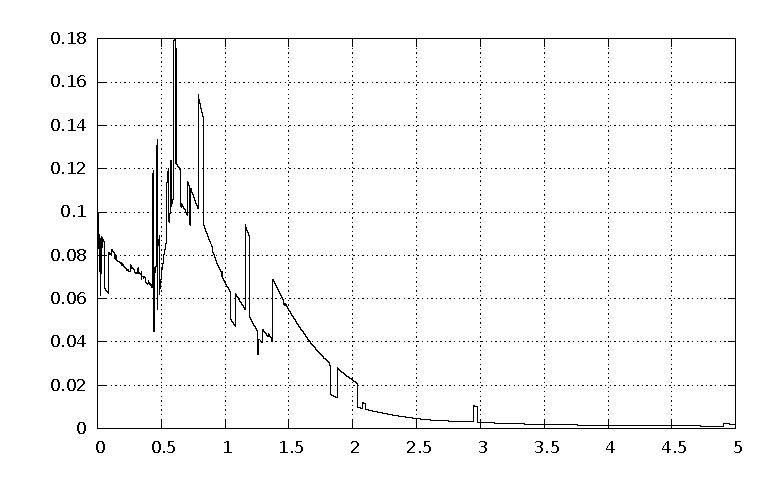
\includegraphics[width=.45\textwidth]
{figures/stokes/nonuniform_bubble_velocity_32_both.ps}
\caption[Stokes equidistribution velocity]
{($\mu=\gamma=1$) $\|\vec U^m\|_{L^\infty(\Omega)}$ evolution for a nonuniform
circle formed by $J_\Gamma = 32$ elements. Here we use the P2--P0 element, and
let $C_v = 3$.}
\label{fig:nonuniform_bubble_velocity_32_both}
\end{figure}

Finally, we would also like to investigate the effect of using an adaptive bulk
mesh, which is more refined close to the interface, and performing only mesh
smoothing. We use $J_\Gamma = 64$ elements for $\Gamma^0$ and $J_\Omega^0 =
954$ elements for the bulk. We see from the evolution in
Figure~\ref{fig:nonuniform_bubble_64_adaptive} that, again, we obtain an
equidistributed approximation of a circle. Obviously, since we never perform a
remesh, the final bulk mesh quality is very poor.
\begin{figure}[htbp]
\centering
\subfloat[$t=0$]{\includegraphics[width=.45\textwidth]
{figures/stokes/nonuniform_bubble_64_coarse_smooth_000.ps}}\\
\subfloat[$t=0.5$]{\includegraphics[width=.45\textwidth]
{figures/stokes/nonuniform_bubble_64_coarse_smooth_050.ps}}
\subfloat[$t=1$]{\includegraphics[width=.45\textwidth]
{figures/stokes/nonuniform_bubble_64_coarse_smooth_100.ps}}\\
\subfloat[$t=2.5$]{\includegraphics[width=.45\textwidth]
{figures/stokes/nonuniform_bubble_64_coarse_smooth_250.ps}}
\subfloat[$t=5$]{\includegraphics[width=.45\textwidth]
{figures/stokes/nonuniform_bubble_64_coarse_smooth_500.ps}}
\caption[Stokes equidistribution property adaptive mesh]
{($\mu=\gamma=1$) Mesh evolution of a nonuniform circle formed by
$J_\Gamma = 64$ elements and adaptive bulk mesh. Here we use the P2--P0
element, and no remeshing.}
\label{fig:nonuniform_bubble_64_adaptive}
\end{figure}
In Figure~\ref{fig:nonuniform_bubble_velocity_64_coarse_smooth} is shown the
evolution of $\|\vec U^m\|_{L^\infty(\Omega)}$ which, again, converges to zero.
\begin{figure}[htbp]
\centering
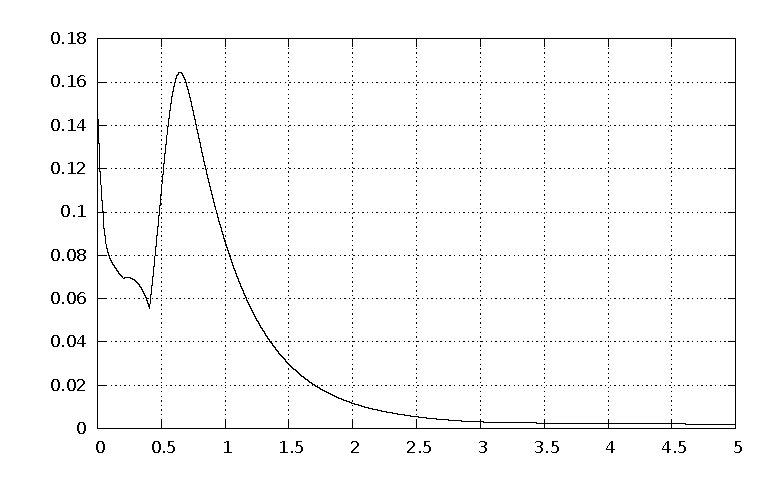
\includegraphics[width=.45\textwidth]
{figures/stokes/nonuniform_bubble_velocity_64_coarse_smooth.ps}
\caption[Stokes equidistribution velocity adaptive mesh]
{($\mu=\gamma=1$) $\|\vec U^m\|_{L^\infty(\Omega)}$ evolution for a nonuniform
circle formed by $J_\Gamma = 64$ elements and adaptive bulk mesh. Here we use
the P2--P0 element, and no remeshing.}
\label{fig:nonuniform_bubble_velocity_64_coarse_smooth}
\end{figure}
We notice that the evolution of the quantity $\|\vec U^m\|_{L^\infty(\Omega)}$
is now very smooth respect to the one reported in
Figure~\ref{fig:nonuniform_bubble_32_both} but this is not surprising since we
never perform a remesh.

\subsection{Energy decay and area conservation in 2d}
In Figure~\ref{fig:ellipse_both} we show the pressure evolution for a
simulation that starts with an initial ellipse, with major and minor axes of
1.6 and 0.75. We use the parameters $\mu = \gamma=1$, $\tau=10^{-2}$ and
$T=10$. The initial interface is discretized with $J_\Gamma = 40$ surface
elements, and the initial bulk mesh has $J_\Omega^0 = 1112$ elements. We employ
the P2--P0 element and use the remeshing parameter $C_v=3$ during the evolution.
Figure~\ref{fig:ellipse_both_volumes} shows the evolution of the relative inner
area $\frac{\mathcal{L}^2(\Omega^m_-)}{\mathcal{L}^2(\Omega^0_-)}$ and the
evolution of the interface energy $\gamma\,\mathcal{H}^{1}(\Gamma^m)$. The
graphs show that the inner area is nearly conserved, and that the interface
energy is monotonically decreasing. We point out that, since there is no exact
solution to the problem, we cannot show the pressure state at time $t=0$
therefore we show the pressure state at $t=10^{-5}$, which is computed with the
help of our scheme with one time step of size $\tau=10^{-5}$.
\begin{figure}[htbp]
\centering
\subfloat[$t=10^{-5}$]{\includegraphics[width=.45\textwidth]
{figures/stokes/ellipse_both_000.ps}}\\
\subfloat[$t=2.5$]{\includegraphics[width=.45\textwidth]
{figures/stokes/ellipse_both_250.ps}}
\subfloat[$t=5$]{\includegraphics[width=.45\textwidth]
{figures/stokes/ellipse_both_500.ps}}\\
\subfloat[$t=7.5$]{\includegraphics[width=.45\textwidth]
{figures/stokes/ellipse_both_750.ps}}
\subfloat[$t=10$]{\includegraphics[width=.45\textwidth]
{figures/stokes/ellipse_both_1000.ps}}
\caption[Stokes ellipse pressure]
{($\mu=\gamma=1$) Pressure evolution of an ellipse that evolves towards a
circle. Here we use the P2--P0 element, and let $C_v = 3$.}
\label{fig:ellipse_both}
\end{figure}
\begin{figure}[htbp]
\centering
\subfloat[$\frac{\mathcal{L}^2(\Omega^m_-)}{\mathcal{L}^2(\Omega^0_-)}$]{
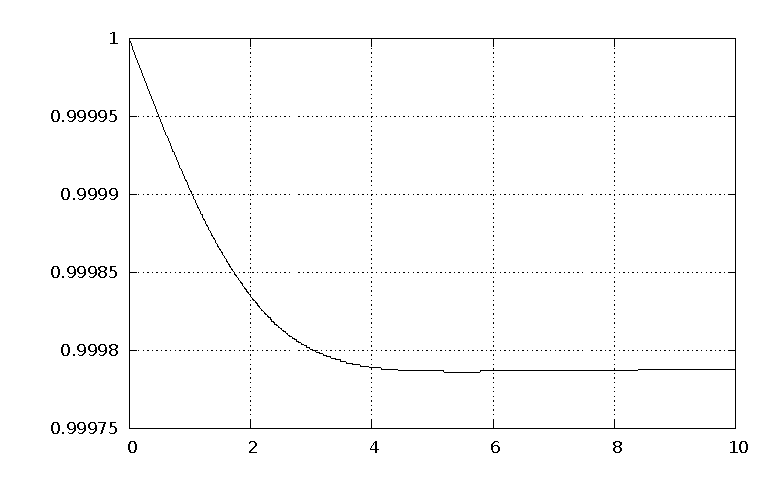
\includegraphics[width=.45\textwidth]
{figures/stokes/ellipse_both_bulk_inner_volume.ps}}
\subfloat[$\gamma\,\mathcal{H}^{1}(\Gamma^m)$]{
\includegraphics[width=.45\textwidth]
{figures/stokes/ellipse_both_interface_length.ps}}
\caption[Stokes ellipse inner area and interface energy]
{Evolutions of the relative inner area and the interface energy for
the simulation in Figure~\ref{fig:ellipse_both}.}
\label{fig:ellipse_both_volumes}
\end{figure}

As a comparison, we show in Figure~\ref{fig:ellipse_smooth} and
\ref{fig:ellipse_both_volumes_smooth} the same simulation when no remeshings are
performed, i.e. we use $C_v=\infty$ in (\ref{eq:volume_criterion}). We clearly
see that due to the strong deformation of the interface, this leads to
elongated elements in the inner and in the outer phase of the bulk finite
element mesh.
\begin{figure}[htbp]
\centering
\subfloat[$t=10^{-5}$]{\includegraphics[width=.45\textwidth]
{figures/stokes/ellipse_smooth_000.ps}}\\
\subfloat[$t=2.5$]{\includegraphics[width=.45\textwidth]
{figures/stokes/ellipse_smooth_250.ps}}
\subfloat[$t=5$]{\includegraphics[width=.45\textwidth]
{figures/stokes/ellipse_smooth_500.ps}}\\
\subfloat[$t=7.5$]{\includegraphics[width=.45\textwidth]
{figures/stokes/ellipse_smooth_750.ps}}
\subfloat[$t=10$]{\includegraphics[width=.45\textwidth]
{figures/stokes/ellipse_smooth_1000.ps}}
\caption[Stokes ellipse pressure no remeshing]
{($\mu=\gamma=1$) Pressure evolution of an ellipse that evolves towards a
circle. Here we use the P2--P0 element, and no remeshing.}
\label{fig:ellipse_smooth}
\end{figure}
\begin{figure}[htbp]
\centering
\subfloat[$\frac{\mathcal{L}^2(\Omega^m_-)}{\mathcal{L}^2(\Omega^0_-)}$]{
\includegraphics[width=.45\textwidth]
{figures/stokes/ellipse_smooth_bulk_inner_volume.ps}}
\subfloat[$\gamma\,\mathcal{H}^{1}(\Gamma^m)$]{
\includegraphics[width=.45\textwidth]
{figures/stokes/ellipse_smooth_interface_length.ps}}
\caption[Stokes ellipse inner area and interface energy no remeshing]
{Evolutions of the relative inner area and the interface energy for
the simulation in Figure~\ref{fig:ellipse_smooth}.}
\label{fig:ellipse_both_volumes_smooth}
\end{figure}

\subsection{Shear flow experiment in 2d}
As the final 2d numerical simulation we present a shear flow experiment. Here
we prescribe the inhomogeneous Dirichlet boundary condition
\begin{equation*}
\vec g(\vec z)=(z_2,0)^T\quad \mbox{on }\partial\Omega\,,
\end{equation*}
and we use the parameters $\mu=1$, $\gamma=3$, $\tau=10^{-2}$ and $T=5$.
The initial interface is discretized with $J_\Gamma = 64$ surface elements,
and the initial bulk mesh has $J_\Omega^0 = 4240$ elements. In
Figure~\ref{fig:shear_2d} we show the evolution of the discrete pressures
for a simulation with $C_v=3$ for the P2--P0 element, while the velocities
are visualized in Figure~\ref{fig:shear_2d_velocity}.
\begin{figure}[htbp]
\centering
\subfloat[$t=0.5$]{\includegraphics[width=.45\textwidth]
{figures/stokes/2d_shear_050.ps}}
\subfloat[$t=1$]{\includegraphics[width=.45\textwidth]
{figures/stokes/2d_shear_100.ps}}\\
\subfloat[$t=2.5$]{\includegraphics[width=.45\textwidth]
{figures/stokes/2d_shear_250.ps}}
\subfloat[$t=5$]{\includegraphics[width=.45\textwidth]
{figures/stokes/2d_shear_500.ps}}
\caption[Stokes 2d shear flow pressure]
{($\mu=1,\gamma=3$) Pressure evolution for the 2d shear flow with $C_v=3$ for
the P2--P0 element, uniform mesh.}
\label{fig:shear_2d}
\end{figure}
\begin{figure}[htbp]
\centering
\subfloat[$t=0.5$]{\includegraphics[width=.45\textwidth]
{figures/stokes/2d_shear_velocity_050.ps}}
\subfloat[$t=1$]{\includegraphics[width=.45\textwidth]
{figures/stokes/2d_shear_velocity_100.ps}}\\
\subfloat[$t=2.5$]{\includegraphics[width=.45\textwidth]
{figures/stokes/2d_shear_velocity_250.ps}}
\subfloat[$t=5$]{\includegraphics[width=.45\textwidth]
{figures/stokes/2d_shear_velocity_500.ps}}
\caption[Stokes 2d shear flow velocity]
{($\mu=1,\gamma=3$) Velocity vector field for the 2d shear flow with $C_v=3$
for the P2--P0 element, uniform mesh.}
\label{fig:shear_2d_velocity}
\end{figure}

A plot of the relative inner area over time is shown in
Figure~\ref{fig:shear_2d_bulk_inner_volume}, where we again observe that our
numerical method maintains the enclosed volume well.
\begin{figure}[htbp]
\centering
\includegraphics[width=.45\textwidth]
{figures/stokes/2d_shear_bulk_inner_volume.ps}
\caption[Stokes 2d shear flow inner area]
{A plot of the relative inner area
$\frac{\mathcal{L}^2(\Omega^m_-)}{\mathcal{L}^2(\Omega^0_-)}$
over time for the simulation in Figure~\ref{fig:shear_2d}.}
\label{fig:shear_2d_bulk_inner_volume}
\end{figure}

Finally we want to compare the performance of different preconditioner
for the preconditioned GMRES used to solve the reduce system
(\ref{eq:SchurkX}) or, depending on the pressure space,
(\ref{eq:SchurkX_extended}). In Table~\ref{tab:shear_2d_preconditioners} we
report the CPU time, in seconds, and the number of GMRES iteration to solve the
algebraic system (\ref{eq:SchurkX_extended}) at the first time step, $m=0$. We
employ uniform bulk meshes and the P2--(P1+P0) element. We test the direct
preconditioner (\ref{eq:stokes_direct_precond_extended}) factorizing it
alternatively with either UMFPACK or SPQR and the block preconditioner
(\ref{eq:ESW_extended}) with restart value either 50 or 1000.
\begin{table*}
\center
\hspace*{-3.25cm}
\begin{tabular}{rrrrrrrrr}
\hline
$J_\Gamma$ & \multicolumn{2}{r}{Direct UMFPACK} &
\multicolumn{2}{r}{Direct SPQR} & \multicolumn{2}{r}{Block restart 50} &
\multicolumn{2}{r}{Block restart 1000} \\
\hline
 & CPU[s] & iterations & CPU[s] & iterations & CPU[s] & iterations & CPU[s] &
iterations \\
\hline
 16 &  0.06 & 6 &  0.13 & 5 &    0.94 &  349 &    1.16 &  221 \\
 32 &  0.33 & 7 &  0.68 & 6 &   11.33 &  839 &   11.51 &  441 \\
 64 &  1.83 & 8 &  4.16 & 8 &  138.58 & 2026 &  136.99 &  772 \\
128 & 10.05 & 9 & 25.71 & 9 & 2079.82 & 6436 & 1442.76 & 1745 \\
\hline
\end{tabular}
\hspace*{-3.25cm}
\caption[Stokes 2d shear flow preconditioners comparison]
{($\mu=1,\gamma=3$) Time and number of GMRES iterations to solve the algebraic
system (\ref{eq:SchurkX_extended}) adopting different preconditioners for the 2d
shear flow using P2--(P1+P0) element, uniform mesh and $m=0$.}
\label{tab:shear_2d_preconditioners}
\end{table*}
We can notice that the direct preconditioner, whose matrix is equivalent to
a standard Stokes discretization perform extremely well in terms of CPU time
and number of GMRES iterations. This is not very surprising since the
preconditioner and the reduced two-phase stokes system have almost the same
matrix. Therefore the number of GMRES iterations is very low. Moreover, the
factorization is computed only once with both SPQR and UMFPACK so it is
extremely efficient to apply the preconditioner at every GMRES iteration. On
the other hand, the block preconditioner perform very poorly requiring a very
high number of GMRES iterations in order to converge. An increase of the
restart value obviously reduce the number of GMRES iterations but also
drastically increase the memory footprint. Moreover, the application of the
preconditioner consist of doing the backward substitution
(\ref{eq:blocksolution_extended}) which is expensive.

\subsection{Convergence test in 3d} \label{sec:stokes_3d_convergence_results}
Similarly to \S\ref{sec:stokes_2d_convergence_results}, we perform the following
convergence test for a stationary spherical bubble in 3d. Let $\mu = \gamma =
1$. Then the true solution (\ref{eq:radialr},b) reduces to $r(t) =
\frac{1}{2}$, $\vec u(\cdot, t) = \vec 0$ and $p(t) = 4\,\charfcn{\Omega_-(0)}
- \frac{\pi}{12}$ for all $t\geq0$. We approximate this stationary solution on
nearly uniform meshes that feature $J_\Gamma = 32$, $220$ and $596$ interface
elements, and $J_\Omega^0 = 408$, $3590$ and $20473$ bulk elements,
respectively. Here, in contrast to the situation in 2d, we are not able to
define $\Gamma^0$ such that the vertices of $\Gamma^0$ lie on $\Gamma(0)$ and
such that (\ref{eq:constcurv}) is satisfied. As we would like to demonstrate
the ability of our method to recover the discrete stationary solution
(\ref{eq:solsol}) also in 3d, we choose the initial interface $\Gamma^0$ such
that (\ref{eq:constcurv}) holds, at the expense of a nonzero initial error
$\| \Gamma^0 - \Gamma(0) \|_{L^\infty}$, recall (\ref{eq:errorXx}). We obtain
such an initial triangulation with the help of the numerical scheme from
Chapter~\ref{ch:geometric_pdes} for surface diffusion, which is a gradient flow
for surface area that maintains the enclosed volume. See e.g. \cite[Fig.
11]{gflows3d} for an evolution towards a polyhedral approximation of a sphere
that satisfies (\ref{eq:constcurv}), and hence also (\ref{eq:conformal}). We
report on the errors for the P2--P0, P2--P1, P2--\pdg
and P2--(P1+P0) elements in Tables~\ref{tab:stokes_stationary_3d_p2p0},
\ref{tab:stokes_stationary_3d_p2p1}, \ref{tab:stokes_stationary_3d_p2p1dg} and
\ref{tab:stokes_stationary_3d_p2p1p0}, respectively. Here we note that, as yet,
for the pairs P2--P0, P2--\pdg and P2--(P1+P0) there exist no proofs in the
literature that the LBB condition (\ref{eq:LBB}) holds, see e.g. the discussion
in \cite[Remark~8.4.3]{BoffiBF13}. However, in practice we encountered no
problems when using these spaces, and our iterative solver always converged to a
solution of the scheme (\ref{eq:HGa}--d). For both sets of simulations we use
the uniform time step size $\tau = 10^{-2}$.
\begin{table*}
\center
\begin{tabular}{rllllr}
\hline
$J_\Gamma$ & $\errorXx$ & $\LerrorUu2$ & $\LerrorPp$ & EOC & CPU[s] \\
\hline
 32 & 2.97986e-02 & 0 & 1.65555e-00 &    - &   385 \\
220 & 5.80971e-03 & 0 & 7.14269e-01 & 1.21 &  4699 \\
596 & 2.42857e-03 & 0 & 3.58466e-01 & 0.99 & 51604 \\
\hline
\end{tabular}
\caption[Stokes 3d stationary bubble errors P2--P0]
{($\mu=\gamma=1$) Stationary bubble problem on $(-1,1)^3$ over the time
interval $[0,1]$ for the P2--P0 element.}
\label{tab:stokes_stationary_3d_p2p0}
\end{table*}
\begin{table*}
\center
\begin{tabular}{rllllr}
\hline
$J_\Gamma$ & $\errorXx$ & $\LerrorUu2$ & $\LerrorPp$ & EOC & CPU[s] \\
\hline
 32 & 1.56938e-01 & 6.01956e-02 & 2.10996e-00 &    - &   315 \\
220 & 7.28946e-02 & 3.13992e-02 & 1.47595e-00 & 0.52 &  4231 \\
596 & 4.04291e-02 & 1.34276e-02 & 1.09674e-00 & 0.43 & 51287 \\
\hline
\end{tabular}
\caption[Stokes 3d stationary bubble errors P2--P1]
{($\mu=\gamma=1$) Stationary bubble problem on $(-1,1)^3$ over the time
interval $[0,1]$ for the P2--P1 element.}
\label{tab:stokes_stationary_3d_p2p1}
\end{table*}
\begin{table*}
\center
\begin{tabular}{rllllr}
\hline
$J_\Gamma$ & $\errorXx$ & $\LerrorUu2$ & $\LerrorPp$ & EOC & CPU[s] \\
\hline
 32 & 2.97986e-02 & 0 & 1.65555e-00 &    - &    73 \\
220 & 5.80971e-03 & 0 & 7.14269e-01 & 1.21 &  1018 \\
596 & 2.42857e-03 & 0 & 3.58466e-01 & 0.99 & 17814 \\
\hline
\end{tabular}
\caption[Stokes 3d stationary bubble errors P2--\pdg]
{($\mu=\gamma=1$) Stationary bubble problem on $(-1,1)^3$ over the time
interval $[0,1]$ for the P2--\pdg element.}
\label{tab:stokes_stationary_3d_p2p1dg}
\end{table*}
\begin{table*}
\center
\begin{tabular}{rllllr}
\hline
$J_\Gamma$ & $\errorXx$ & $\LerrorUu2$ & $\LerrorPp$ & EOC & CPU[s] \\
\hline
 32 & 2.97986e-02 & 0 & 1.65749e-00 &    - &    568 \\
220 & 5.80971e-03 & 0 & 7.15353e-01 & 1.21 &   9174 \\
596 & 2.42857e-03 & 0 & 3.59181e-01 & 0.99 & 121110 \\
\hline
\end{tabular}
\caption[Stokes 3d stationary bubble errors P2--(P1+P0)]
{($\mu=\gamma=1$) Stationary bubble problem on $(-1,1)^3$ over the time
interval $[0,1]$ for the P2--(P1+P0) element.}
\label{tab:stokes_stationary_3d_p2p1p0}
\end{table*}

We note that we again recover the discrete stationary solutions
(\ref{eq:solsol}) for the P2--P0, P2--\pdg and P2--(P1+P0) elements while,
as before, the P2--P1 element does not capture exactly the true solution
since this element does not satisfy the hypothesis that
$\charfcn{\Omega^m_-}\in\pspace^m$ of Theorem~\ref{thm:stat2}. Here this leads
to a nonzero error in the position of the discrete interface, because the
vertices of the initial interface $\Gamma^0$ do not lie on $\Gamma(0)$.

\subsection{Shear flow experiment in 3d}
Finally, we also report on a 3d shear flow experiment.
The initial interface mesh has $J_\Gamma = 596$ elements, while the nearly
uniform bulk mesh is made up of $J_\Omega^0 = 19641$ elements. We prescribe the
inhomogeneous Dirichlet boundary condition
\begin{equation*}
\vec g(\vec z)=(z_3,0,0)^T\quad \mbox{on }\partial\Omega\,,
\end{equation*}
and we use the parameters $\mu=1$, $\gamma=3$, $\tau=10^{-2}$ and $T=5$.
In Figure~\ref{fig:shear_3d} we show the evolution of the discrete interface
for a simulation with $C_v=3$ for the P2--P0 element, while the velocities
are visualized in Figure~\ref{fig:shear_3d_velocity}.
\begin{figure}[htbp]
\centering
\subfloat[$t=0$]{\includegraphics[width=.45\textwidth]
{figures/stokes/3d_shear_000.ps}}\\
\subfloat[$t=0.5$]{\includegraphics[width=.45\textwidth]
{figures/stokes/3d_shear_050.ps}}
\subfloat[$t=1$]{\includegraphics[width=.45\textwidth]
{figures/stokes/3d_shear_100.ps}}\\
\subfloat[$t=2.5$]{\includegraphics[width=.45\textwidth]
{figures/stokes/3d_shear_250.ps}}
\subfloat[$t=5$]{\includegraphics[width=.45\textwidth]
{figures/stokes/3d_shear_500.ps}}
\caption[Stokes 3d shear flow interface]
{($\mu=1,\gamma=3$) Interface evolution for the 3d shear flow with $C_v=3$ for
the P2--P0 element, uniform mesh.}
\label{fig:shear_3d}
\end{figure}
\begin{figure}[htbp]
\centering
\subfloat[$t=0.5$]{\includegraphics[width=.45\textwidth]
{figures/stokes/3d_shear_velocity_050.ps}}
\subfloat[$t=1$]{\includegraphics[width=.45\textwidth]
{figures/stokes/3d_shear_velocity_100.ps}}\\
\subfloat[$t=2.5$]{\includegraphics[width=.45\textwidth]
{figures/stokes/3d_shear_velocity_250.ps}}
\subfloat[$t=5$]{\includegraphics[width=.45\textwidth]
{figures/stokes/3d_shear_velocity_500.ps}}
\caption[Stokes 3d shear flow velocity]
{($\mu=1,\gamma=3$) Velocity vector field in the plane normal to $(0,1,0)^T$
and passing through the origin for the 3d shear flow with $C_v=3$ for the
P2--P0 element, uniform mesh.}
\label{fig:shear_3d_velocity}
\end{figure}

A plot of the relative inner volume over time is shown in
Figure~\ref{fig:shear_3d_bulk_inner_volume}, where we again observe that our
numerical method maintains the enclosed volume well.
\begin{figure}[htbp]
\centering
\includegraphics[width=.45\textwidth]
{figures/stokes/3d_shear_bulk_inner_volume.ps}
\caption[Stokes 3d shear flow inner volume]
{A plot of the relative inner volume
$\frac{\mathcal{L}^3(\Omega^m_-)}{\mathcal{L}^3(\Omega^0_-)}$
over time for the simulation in Figure~\ref{fig:shear_3d}.}
\label{fig:shear_3d_bulk_inner_volume}
\end{figure}

Finally, as in the 2d case, see Table~\ref{tab:shear_2d_preconditioners}, we
want to compare the performance of different preconditioners. In
Table~\ref{tab:shear_3d_preconditioners} we report the CPU time, in seconds,
and the number of GMRES iteration to solve the algebraic system
(\ref{eq:SchurkX_extended}) at the first time step, $m=0$. We employ adaptive
bulk meshes and the P2--(P1+P0) element. We test the direct preconditioner
(\ref{eq:stokes_direct_precond_extended}) factorizing it alternatively with
either UMFPACK or SPQR and the block preconditioner (\ref{eq:ESW_extended})
with restart value either 50 or 1000.
\begin{table*}
\center
\hspace*{-3.25cm}
\begin{tabular}{rrrrrrrrr}
\hline
$J_\Gamma$ & \multicolumn{2}{r}{Direct UMFPACK} &
\multicolumn{2}{r}{Direct SPQR} & \multicolumn{2}{r}{Block restart 50} &
\multicolumn{2}{r}{Block restart 1000} \\
\hline
 & CPU[s] & iterations & CPU[s] & iterations & CPU[s] & iterations & CPU[s] &
iterations \\
\hline
 32 &  0.16 & 8 &  0.26 & 5 &   1.10 & 158 &  1.17 & 130 \\
220 &  3.56 & 7 &  4.91 & 6 &  15.31 & 234 & 14.53 & 193 \\
596 & 13.77 & 6 & 44.44 & 6 & 101.53 & 328 & 93.00 & 266 \\
\hline
\end{tabular}
\hspace*{-3.25cm}
\caption[Stokes 3d shear flow preconditioners comparison]
{($\mu=1,\gamma=3$) Time and number of GMRES iterations to solve the algebraic
system (\ref{eq:SchurkX_extended}) adopting different preconditioners for the 3d
shear flow using P2--(P1+P0) element, adaptive mesh and $m=0$.}
\label{tab:shear_3d_preconditioners}
\end{table*}
We observe that also in 3d the direct preconditioners outperform the block
preconditioner both in term of GMRES iterations and CPU time.
\chapter{\sc Two-Phase Stokes Flow Numerical Results}\label{ch:stokes_results}
In order to test our method, and to allow comparisons with the unfitted finite
element approximation in \cite{spurious}, we now present several numerical
experiments in 2d and 3d. This chapter is extensively based on a paper we
wrote, see \cite{stokesfitted}.

The chapter is organised as follows: in \S\ref{sec:stokes_exact_solutions} we
state two exact solutions to the two-phase Stokes problem and we verify that
they are indeed solutions; in \S\ref{sec:errors} we describe the general
settings for the simulations and we define the error estimators used; in
\S\ref{sec:stokes_2d_convergence_results} we report on the convergence test in
2d; in \S\ref{sec:stokes_2d_equidistributon} we show that interface mesh points
are naturally equidistributed by our scheme; in \S\ref{sec:stokes_2d_energy} we
show that our scheme conserve the enclosed volume and that the surface energy
monotonically decays; in \S\ref{sec:stokes_2d_shear} we present a shear
flow experiment in 2d; in \S\ref{sec:stokes_3d_convergence_results} we report on
the convergence test in 3d; in \S\ref{sec:stokes_3d_shear} we finally present a
shear flow experiment in 3d.

\section{Exact solutions}\label{sec:stokes_exact_solutions}
We recall the following stationary and expanding spherical solutions
from \cite{spurious}. Let $\Gamma(t) = \{ \vec z \in \R^d : |\vec z\,| = r(t)\}$
be a sphere of radius $r(t)$  and mean curvature $\varkappa(t) =
-\frac{d-1}{r(t)}$. Moreover let $\alpha,\gamma\in \R_{\geq 0}$ be given. We
will refer to (\ref{eq:radialr},b) as the stationary bubble solution, and to
(\ref{eq:radialr2},b) as the expanding bubble solution.

\subsection{Stationary bubble}\label{sec:stokes_stationary}
The stationary sphere where
\begin{subequations}
\begin{equation} \label{eq:radialr}
r(t) = r(0)\,,
\end{equation}
together with
\begin{equation} \label{eq:radialup}
\vec u(\vec z, t) = \vec 0 \,,\quad p(\vec z, t) =
-\,\gamma \varkappa(0)\left[\charfcn{\Omega_-(0)}
-\frac{\vol(\Omega_-(0))}{\vol(\Omega)} \right] ,
\end{equation}
\end{subequations}
is an exact solution to the problem (\ref{eq:stokes_full_momentum}--h) on e.g.\
$\Omega = (-1,1)^d$ with $\vec f=\vec 0$ and $\vec g = \vec 0$ on
$\partial_1\Omega=\partial\Omega$. This solution is the continuous version of
(\ref{eq:solsol}).

It is trivial to verify that (\ref{eq:radialr},b) is indeed an exact solution.
Firstly, given that the velocity $\vec u$ is zero and the pressure $p$ is
constant in each phase, the momentum equation (\ref{eq:stokes_full_momentum})
automatically holds if $\vec f=\vec 0$ and the continuity equation
(\ref{eq:stokes_full_mass}) is satisfied. Moreover, also the stress balance
(\ref{eq:stokes_full_jump_stress}) holds since, substituting
(\ref{eq:radialup}) in (\ref{eq:stokes_full_jump_stress}), we obtain
\begin{align*}
\big[2\,\mu \mat D(\vec u)\,.\,\vec\nu - p\,\vec \nu\big]_-^+ =
& \big[- p\,\vec \nu\big]_-^+ \\
= & -\gamma \varkappa(0)\frac{\vol(\Omega_-(0))}{\vol(\Omega)}\vec \nu
-\gamma \varkappa(0) \vec \nu +
\gamma \varkappa(0)\frac{\vol(\Omega_-(0))}{\vol(\Omega)}\vec \nu \\
= & -\gamma \varkappa(0)\vec \nu = -\gamma\varkappa \vec\nu\,.
\end{align*}
Finally, the dynamic interface condition (\ref{eq:stokes_full_velocity}) is
trivially satisfied since the interface is stationary and $\vec u$ is zero.

\subsection{Expanding bubble}\label{sec:stokes_expanding}
A nontrivial divergence free and radially symmetric solution $\vec u$ can be
constructed on a domain that does not contain the origin. To this end, consider
e.g. $\Omega = (-1,1)^d \setminus [-\frac13,\frac13]^d$. Then, the expanding
sphere where
\begin{subequations}
\begin{equation} \label{eq:radialr2}
r(t) = ([r(0)]^d + \alpha\,t\,d)^\frac1d \,,
\end{equation}
together with
\begin{equation} \label{eq:radialup2}
\vec u(\vec z, t) = \alpha\,\frac{\vec z}{|\vec z\,|^d}\,, \quad
p(\vec z, t) = -\,\bigg(\gamma +2\,\alpha\,\frac{\mu_+ - \mu_-}
{r(t)^{d-1}}\bigg)\,\varkappa(t)\,\left[ \charfcn{\Omega_-(t)} -
\frac{\vol(\Omega_-(t))}{\vol(\Omega)}\right],
\end{equation}
\end{subequations}
is an exact solution to the problem (\ref{eq:stokes_full_momentum}--h) with
$\vec f = \vec 0$ and $\vec g(\vec z) = \alpha\,|\vec z\,|^{-d}\,\vec z$ on
$\partial_1\Omega=\partial\Omega$.

We now verify that (\ref{eq:radialr2},b) is indeed an exact solution. Firstly,
we have that
\begin{equation*}
\frac{\partial u_i}{\partial z_j}=\alpha\frac{\delta_{ij}
- d z_i z_j |\vec z\,|^{-2}}{|\vec z\,|^d}
\end{equation*}
and
\begin{equation*}
\frac{\partial^2 u_i}{\partial z_j^2}=\alpha d
\frac{-2\delta_{ij}z_j-z_i + (d+2)z_i z_j^2|\vec z\,|^{-2}}{|\vec z\,|^{d+2}}\,.
\end{equation*}
Since $\frac{\partial u_i}{\partial z_j}=\frac{\partial u_j}{\partial z_i}$,
the components of the rate-of-deformation tensor are simply
\begin{equation*}
\big[\mat D(\vec u) \big]_{ij} = \frac{1}{2}\bigg(\frac{\partial
u_i}{\partial z_j} + \frac{\partial u_j}{\partial z_i}\bigg)=\frac{\partial
u_i}{\partial z_j}\,.
\end{equation*}
Then, it holds
\begin{align*}
\big[\nabla\,.\,\mat D(\vec u)\big]_i = &
\sum_{j=1}^d\frac{\partial}{\partial z_j} \frac{\partial u_i}{\partial z_j}
= \frac{\alpha d}{|\vec z\,|^{d+2}}\sum_{j=1}^d\big(-2\delta_{ij}z_j- z_i
+(d+2)z_i z_j^2 |\vec z\,|^{-2}\big)\\
= & \frac{\alpha d}{|\vec z\,|^{d+2}}\big(-2z_i- dz_i+(d+2)z_i\big)=0\,.
\end{align*}
Therefore, given that the pressure $p$ is constant in each phase, the momentum
equation (\ref{eq:stokes_full_momentum}) holds if $\vec f=\vec 0$. Also the
continuity equation (\ref{eq:stokes_full_mass}) is satisfied since we have
\begin{equation*}
\nabla\,.\,\vec u=\sum_{j=1}^d\frac{\partial u_j}{\partial z_j} =
\sum_{j=1}^d\alpha\frac{1 - d z^2_j|\vec z\,|^{-2}}{|\vec z \,|^d} =
\frac{\alpha}{|\vec z\,|^d} \big(d - d |\vec z\,|^2|\vec z\,|^{-2}\big) = 0\,.
\end{equation*}
Moreover, also the stress balance
(\ref{eq:stokes_full_jump_stress}) holds since, substituting
(\ref{eq:radialup2}) in (\ref{eq:stokes_full_jump_stress}), we obtain for the
$i$ component
\begin{align*}
& \bigg[\big[2\,\mu \mat D(\vec u)\,.\,\vec\nu - p\,\vec \nu\big]_i\bigg]_-^+ =
\bigg[2\,\mu \sum_{j=1}^d\frac{\partial u_i}{\partial z_j}\nu_j -
p\nu_i\bigg]_-^+
= \bigg[2\,\mu\sum_{j=1}^d\frac{\partial u_i}{\partial z_j}
\frac{z_j}{|\vec z\,|}\bigg]_-^+ -\big[ p\nu_i\big]_-^+ \\
& \qquad = \bigg[2\,\mu\sum_{j=1}^d\bigg(\alpha \frac{\delta_{ij}z_j-dz_iz_j^2|
\vec z\,|^{-2}}{|\vec z\,|^{d+1}}\bigg)\bigg]_-^+
-\bigg(\gamma +2 \,\alpha \frac{\mu_+ - \mu_-}{r^{d-1}}\bigg)\varkappa\nu_i \\
& \qquad = \bigg[2\,\mu \,\alpha \frac{z_i-dz_i}{|\vec z\,|^{d+1}}\bigg]_-^+
-\gamma \varkappa \nu_i - 2\,\alpha\frac{\mu_+ -
\mu_-}{|\vec z\,|^{d-1}}\frac{1-d}{|\vec z\,|}\frac{z_i}{|\vec z\,|} \\
& \qquad = 2\,\alpha \frac{(\mu_+-\mu_-)(1-d)z_i}{|\vec z\,|^{d+1}}
-\gamma \varkappa \nu_i - 2\,\alpha\frac{(\mu_+-\mu_-)(1-d)z_i}{|\vec
z\,|^{d+1}} = -\gamma \varkappa \nu_i\,.
\end{align*}
Finally, the dynamic interface condition (\ref{eq:stokes_full_velocity}) is
satisfied since the fluid velocity on the interface along the normal direction
is
\begin{equation*}
\vec u\,.\,\vec \nu \!\mid_\Gamma=\alpha\frac{\vec z}{|\vec z \,|^d}\,.\,
\frac{\vec z}{|\vec z \,|}=\alpha\frac{r^2}{r^{d+1}}=\alpha r^{1-d}\,,
\end{equation*}
while the interface velocity along the normal direction is
\begin{equation*}
\V\,.\,\vec \nu=r^\prime=\alpha r^{1-d}\,,
\end{equation*}
where we have used
\begin{equation*}
r^d=r_0^d+\alpha t d \iff d r^{d-1}r^\prime=\alpha d \iff r^\prime=\alpha
r^{1-d}\,,
\end{equation*}
with $r_0=r(0)$.

\section{Settings and error estimators}\label{sec:errors}
In our numerical simulations, unless otherwise stated, we use the following
settings. We choose the initial surface $\Gamma(0) = \{ \vec z \in \R^d : |\vec
z\,| = \frac12 \}$, the domain $\Omega = (-1,1)^d$ and we employ uniform time
steps $\tau_m=\tau$, $m=0,\ldots, M-1$. We compute the discrete solutions
over the time interval $[0,1]$. Moreover, we set the GMRES tolerance to
tol $=10^{-12}$ and the restart value to 50. We use the Stokes matrix
(\ref{eq:stokes_direct_precond}) or, depending on the pressure space,
(\ref{eq:stokes_direct_precond_extended}) as a preconditioner factorizing it
with UMFPACK. We point out that the restart value corresponds to the size
of the Krylov subspace used by the GMRES method while the tolerance is the
value for the stopping criterion. More precisely, the GMRES iteration ends when
the ratio between the norm of the preconditioned actual residual and the norm
of the preconditioned initial residual is smaller than the required tolerance.

We define the errors
\begin{equation} \label{eq:errorXx}
\errorXx := \max_{m=1,\ldots, M} \|\Gamma^m - \Gamma(t_m)\|_{L^\infty}\,,
\end{equation}
where $\|\Gamma^m - \Gamma(t_m)\|_{L^\infty} :=
\max_{k=1,\ldots, K_\Gamma} {\rm dist}( \vec q^m_k, \Gamma(t_m))$,
\begin{equation} \label{eq:errorLUu}
\LerrorUu2 := \left[\tau\,\sum_{m=1}^M \|\vec U^m - I^m_2\,\vec u(\cdot,
t_m)\|_{L^2(\Omega)}^2 \right]^\frac12,
\end{equation}
\begin{equation} \label{eq:errorHUu}
\HerrorUu2 := \left[\tau\,\sum_{m=1}^M \|\vec U^m - I^m_2\,\vec u(\cdot,
t_m)\|_{H^1(\Omega)}^2 \right]^\frac12,
\end{equation}
and
\begin{equation} \label{eq:errorPp}
\LerrorPp := \left[\tau\,\sum_{m=1}^M \|P^m - p(\cdot,t_m)\|_{L^2(\Omega)}^2
\right]^\frac12.
\end{equation}
In (\ref{eq:errorPp}) we employ a quadrature rule of degree $k$, with $k=13$ in
2d and $k=10$ in 3d, to compute the $L^2$--norms over $\Omega$.

Finally, we also define the estimated error of convergence EOC as
\begin{equation} \label{eq:eoc}
\mbox{EOC}=\frac{\ln{\frac{\mbox{error}_1}{\mbox{error}_0}}}
{\ln{\frac{\mbox{h}_1}{\mbox{h}_0}}}\,,
\end{equation}
where $\mbox{error}_1$ is the error computed on a triangulation finer that the
one used to compute $\mbox{error}_0$ while $\mbox{h}_1$ and $\mbox{h}_0$ are the
respective characteristic lengths.

\section{Convergence tests in 2d}\label{sec:stokes_2d_convergence_results}
For the true solution (\ref{eq:radialr},b) we choose $\mu = \gamma = 1$.
Therefore, the solution reduces to $r(t) =
\frac{1}{2}$, $\vec u(\cdot, t) = \vec 0$ and $p(t) = 2\,\charfcn{\Omega_-(0)} -
\frac{\pi}{8}$ for all $t \geq 0$. We approximate this stationary solution on
nearly uniform meshes that feature $J_\Gamma = 2^i$, $i=4,\ldots,7$, uniform
interface elements and $J_\Omega^0 = 224$, $1076$, $4240$, $17194$ bulk
elements, respectively. We show the initial mesh for $J_\Gamma = 32$ in
Figure~\ref{fig:meshes_uniform}.
\begin{figure}[htbp]
\centering
\includegraphics[width=.45\textwidth]{figures/stokes/mesh_uniform.ps}
\caption[Stokes 2d stationary bubble initial mesh]
{Initial mesh for the 2d stationary bubble problem with $J_\Gamma = 32$
interface elements.}
\label{fig:meshes_uniform}
\end{figure}
In addition, we use a uniform time step size $\tau=10^{-2}$.
We report on the errors for the P2--P0, P2--P1, P2--\pdg
and P2--(P1+P0) elements in Tables~\ref{tab:stokes_stationary_2d_p2p0},
\ref{tab:stokes_stationary_2d_p2p1}, \ref{tab:stokes_stationary_2d_p2p1dg} and
\ref{tab:stokes_stationary_2d_p2p1p0}, respectively.
\begin{table*}
\center
\begin{tabular}{rllllr}
\hline
$J_\Gamma$ & $\errorXx$ & $\LerrorUu2$ & $\LerrorPp$ & EOC & CPU[s] \\
\hline
 16 & 0 & 0 & 3.22254e-01 &    - &    9 \\
 32 & 0 & 0 & 1.41195e-01 & 0.90 &   54 \\
 64 & 0 & 0 & 4.06438e-02 & 1.80 &  292 \\
128 & 0 & 0 & 2.60448e-02 & 0.64 & 1443 \\
\hline
\end{tabular}
\caption[Stokes 2d stationary bubble errors P2--P0]
{($\mu=\gamma=1$) Stationary bubble problem on $(-1,1)^2$ over the time
interval $[0,1]$ for the P2--P0 element.}
\label{tab:stokes_stationary_2d_p2p0}
\end{table*}
\begin{table*}
\center
\begin{tabular}{rllllr}
\hline
$J_\Gamma$ & $\errorXx$ & $\LerrorUu2$ & $\LerrorPp$ & EOC & CPU[s] \\
\hline
 16 & 2.41133e-02 & 9.35478e-03 & 5.75614e-01 &    - &    5 \\
 32 & 1.21789e-02 & 3.44473e-03 & 3.99457e-01 & 0.40 &   36 \\
 64 & 6.17055e-03 & 1.24629e-03 & 2.77632e-01 & 0.52 &  170 \\
128 & 2.97451e-03 & 4.41980e-04 & 1.96901e-01 & 0.50 & 1343 \\
\hline
\end{tabular}
\caption[Stokes 2d stationary bubble errors P2--P1]
{($\mu=\gamma=1$) Stationary bubble problem on $(-1,1)^2$ over the time
interval $[0,1]$ for the P2--P1 element.}
\label{tab:stokes_stationary_2d_p2p1}
\end{table*}
\begin{table*}
\center
\begin{tabular}{rllllr}
\hline
$J_\Gamma$ & $\errorXx$ & $\LerrorUu2$ & $\LerrorPp$ & EOC & CPU[s] \\
\hline
 16 & 0 & 0 & 3.22254e-01 &    - &    8 \\
 32 & 0 & 0 & 1.41195e-01 & 0.90 &   42 \\
 64 & 0 & 0 & 4.06438e-02 & 1.80 &  181 \\
128 & 0 & 0 & 2.60448e-02 & 0.64 & 1006 \\
\hline
\end{tabular}
\caption[Stokes 2d stationary bubble errors P2--\pdg]
{($\mu=\gamma=1$) Stationary bubble problem on $(-1,1)^2$ over the time
interval $[0,1]$ for the P2--\pdg element.}
\label{tab:stokes_stationary_2d_p2p1dg}
\end{table*}
\begin{table*}
 \center
\begin{tabular}{rllllr}
\hline
$J_\Gamma$ & $\errorXx$ & $\LerrorUu2$ & $\LerrorPp$ & EOC & CPU[s] \\
\hline
 16 & 0 & 0 & 3.22254e-01 &    - &   13 \\
 32 & 0 & 0 & 1.41195e-01 & 0.90 &   44 \\
 64 & 0 & 0 & 4.06438e-02 & 1.80 &  203 \\
128 & 0 & 0 & 2.60448e-02 & 0.64 & 2151 \\
\hline
\end{tabular}
\caption[Stokes 2d stationary bubble errors P2--(P1+P0)]
{($\mu=\gamma=1$) Stationary bubble problem on $(-1,1)^2$ over the time
interval $[0,1]$ for the P2--(P1+P0) element.}
\label{tab:stokes_stationary_2d_p2p1p0}
\end{table*}

We can clearly see that the stationary nature of the true solution
(\ref{eq:radialr},b) is captured exactly by our numerical method with the
P2--P0, the P2--\pdg and the P2--(P1+P0) element, see also
Figure~\ref{fig:2d_stationary_bubble} for a visualization of the discrete
pressure in the case $J_\Gamma = 32$. This is not surprising given the
result of Theorem~\ref{thm:stat2}, and the fact that we use an equidistributed
approximation $\Gamma^0$, which means that (\ref{eq:constcurv}) is satisfied.
Instead the element P2--P1 does not satisfy the hypothesis that
$\charfcn{\Omega^m_-}\in\pspace^m$ of Theorem~\ref{thm:stat2} and therefore the
true solution is not captured exactly. Moreover, since
$\charfcn{\Omega_-^h(t)}\not\in \mbox{ P1}$, the volume conservation property
of the semidiscrete scheme (\ref{eq:stokes_volume_semidiscrete}) does not hold
which implies that the P2--P1 element does not conserve the enclosed volume. Of
course, since the discrete solution is stationary, neither smoothing nor
remeshing is performed for the simulations in
Tables~\ref{tab:stokes_stationary_2d_p2p0},
\ref{tab:stokes_stationary_2d_p2p1}, \ref{tab:stokes_stationary_2d_p2p1dg} and
\ref{tab:stokes_stationary_2d_p2p1p0}. We also observe that the error for the
three approximations with the P2--P0, the P2--\pdg and the P2--(P1+P0)
element, respectively, produce identical errors. Again, that is to be expected,
since the pressure solution (\ref{eq:solsol})
\begin{equation*}
P^{m+1} = -\gamma\,\overline\kappa\left[\charfcn{\Omega_-^m}
- \frac{\vol(\Omega_-^m)}{\vol(\Omega)}\right]
\end{equation*}
is such that $P^{m+1}$ is independent of $\pspace^m$, and so the additional
degrees of freedom are not utilized by the pressure approximation.
\begin{figure}[htbp]
\centering
\includegraphics[width=.45\textwidth]
{figures/stokes/2d_stationary_bubble_uniform_100.ps}
\caption[Stokes 2d stationary bubble pressure]
{($\mu=\gamma=1$) Pressure of the 2d stationary bubble at time $t=1$
for the P2--P0 element with $J_\Gamma = 32$ interface elements.}
\label{fig:2d_stationary_bubble}
\end{figure}

For the expanding bubble test, we fix $\Omega = (-1,1)^2 \setminus
[-\frac13,\frac13]^2$ and we choose the parameters $\alpha = 0.15$ and $\mu_+ =
10\,\mu_- = \gamma = 1$ for the true solution (\ref{eq:radialr2},b). Here we
consider two different bulk mesh strategies. Either we use a nearly uniform
mesh, as shown on the left of Figure~\ref{fig:meshes_expanding}, or an adaptive
mesh that uses a finer resolution close to the interface, see the example mesh
on the right-hand side of Figure~\ref{fig:meshes_expanding}.
\begin{figure}[htbp]
\centering
\subfloat[Uniform mesh with $J_\Gamma = 32$]{
\includegraphics[width=.45\textwidth]{figures/stokes/mesh_hole_uniform.ps}}
\subfloat[Adaptive mesh with $J_\Gamma = 64$]{
\includegraphics[width=.45\textwidth]{figures/stokes/mesh_hole_adaptive.ps}}
\caption[Stokes 2d expanding bubble initial meshes]
{Initial meshes for the expanding bubble problem.}
\label{fig:meshes_expanding}
\end{figure}

Details on the discretization parameters for the nearly uniform meshes are
given in Table~\ref{tab:expandingbubble2Delements}. Here we explicitly
state the final number of bulk elements, $J_\Omega^M$, in the case $C_v = 1$
and $C_v = 3$, recall the volume criterion (\ref{eq:volume_criterion}), for the
P2--P0 element. In the former the bulk is remeshed after every time step while
in the latter the bulk is remeshed when the max--min entity volume ratio is
bigger than 3. Of course, when only smoothing is employed, then the number of
bulk mesh elements is invariant, and so $J_\Omega^M = J_\Omega^0$.
\begin{table*}
\center
\begin{tabular}{rrrrr}
\hline
$J_\Gamma$ & $J_\Omega^0$ & $\tau$ & $J_\Omega^M$ for $C_v=1$ &
$J_\Omega^M$ for $C_v=3$ \\
\hline
 16 &   316 & $1.6\cdot10^{-2}$ &  120 &  184 \\
 32 &  1016 &   $4\cdot10^{-3}$ &  452 &  468 \\
 64 &  3916 &         $10^{-3}$ & 1864 & 1858 \\
128 & 15784 & $2.5\cdot10^{-4}$ & 7264 & 7263 \\
\hline
\end{tabular}
\caption[Stokes expanding bubble uniform meshes parameters]
{Discretization parameters for the 2d expanding bubble problem, nearly uniform
meshes.}
\label{tab:expandingbubble2Delements}
\end{table*}
We report on the error for the P2--P0, the P2--\pdg and the P2--(P1+P0)
element in Table~\ref{tab:expandingbubble2Dp2p0},
\ref{tab:expandingbubble2Dp2p1dg} and \ref{tab:expandingbubble2Dp2p1p0},
respectively. On the top part of the tables only mesh smoothings are applied,
in the central part the bulk mesh is remeshed after every time step while at
the bottom the bulk mesh is remeshed only when the volume criterion
(\ref{eq:volume_criterion}), with $C_v=3$, is not satisfied.
\begin{table*}
\center
\hspace*{-3.25cm}
\begin{tabular}{rllllllr}
\hline
$J_\Gamma$ & $\errorXx$ & $\LerrorUu2$ & EOC & $\HerrorUu2$ & $\LerrorPp$ & EOC
& CPU[s] \\
\hline
& \multicolumn{7}{c}{no remeshing} \\
\hline
 16 & 5.94637e-03 & 7.26038e-04 &    - & 1.98118e-02 & 4.30560e-01 &    - &
9 \\
 32 & 1.47959e-03 & 3.39540e-04 & 0.83 & 1.17665e-02 & 2.27294e-01 & 0.70 &
98 \\
 64 & 3.68960e-04 & 8.66188e-05 & 1.97 & 5.82989e-03 & 1.05041e-01 & 1.11 &
1709 \\
128 & 9.20414e-05 & 5.87165e-05 & 0.56 & 6.24063e-03 & 3.18072e-02 & 1.72 &
37539 \\
\hline
& \multicolumn{7}{c}{$C_v=1$} \\
\hline
 16 & 5.92441e-03 & 5.27627e-04 &    - & 1.57505e-02 & 4.43442e-01 &    - &
59 \\
 32 & 1.46657e-03 & 1.05800e-04 & 1.75 & 5.26275e-03 & 2.14680e-01 & 0.79 &
100 \\
 64 & 3.65433e-04 & 1.48680e-05 & 2.83 & 1.50695e-03 & 8.14177e-02 & 1.40 &
2785 \\
128 & 9.12526e-05 & 1.81107e-06 & 3.04 & 3.59374e-04 & 3.69593e-02 & 1.14 &
23465 \\
\hline
& \multicolumn{7}{c}{$C_v=3$} \\
\hline
 16 & 5.94589e-03 & 5.71201e-04 &    - & 1.51195e-02 & 4.44395e-01 &    - &
41 \\
 32 & 1.47176e-03 & 1.02091e-04 & 1.88 & 4.86975e-03 & 2.13617e-01 & 0.80 &
92 \\
 64 & 3.65488e-04 & 1.50366e-05 & 2.76 & 1.50058e-03 & 8.22797e-02 & 1.38 &
1847 \\
128 & 9.12406e-05 & 1.81327e-06 & 3.05 & 3.59347e-04 & 3.69473e-02 & 1.16 &
26973 \\
\hline
\end{tabular}
\hspace*{-3.25cm}
\caption[Stokes expanding bubble uniform mesh errors P2--P0]
{($\mu_+ = 10\,\mu_- = \gamma = 1,\alpha = 0.15$) Expanding bubble
problem on $(-1,1)^2\setminus[-\frac{1}{3},\frac{1}{3}]^2$ over the time
interval $[0,1]$ for the P2--P0 element with nearly uniform mesh.}
\label{tab:expandingbubble2Dp2p0}
\end{table*}
\begin{table*}
\center
\hspace*{-3.25cm}
\begin{tabular}{rllllllr}
\hline
$J_\Gamma$ & $\errorXx$ & $\LerrorUu2$ & EOC & $\HerrorUu2$ & $\LerrorPp$ & EOC
& CPU[s] \\
\hline
& \multicolumn{7}{c}{no remeshing} \\
\hline
 16 & 5.99881e-03 & 1.42557e-03 &    - & 3.45859e-02 & 4.31784e-01 &    - &
9 \\
 32 & 1.47936e-03 & 4.11514e-04 & 1.36 & 1.28088e-02 & 2.27350e-01 & 0.70 &
82 \\
 64 & 3.69030e-04 & 1.03424e-04 & 1.99 & 6.17291e-03 & 1.05060e-01 & 1.11 &
1391 \\
128 & 9.21619e-05 & 6.12532e-05 & 0.76 & 6.21616e-03 & 3.17967e-02 & 1.72 &
31042 \\
\hline
& \multicolumn{7}{c}{$C_v=1$} \\
\hline
 16 & 5.95848e-03 & 8.38757e-04 &    - & 2.23968e-02 & 4.44061e-01 &    - &
100 \\
 32 & 1.47123e-03 & 2.22736e-04 & 1.45 & 7.70628e-03 & 2.15081e-01 & 0.79 &
728 \\
 64 & 3.65750e-04 & 2.16681e-05 & 3.36 & 1.76987e-03 & 8.15608e-02 & 1.40 &
3050 \\
128 & 9.12893e-05 & 2.33116e-06 & 3.22 & 3.96930e-04 & 3.69418e-02 & 1.14 &
25348 \\
\hline
& \multicolumn{7}{c}{$C_v=3$} \\
\hline
 16 & 5.99703e-03 & 8.59166e-04 &    - & 2.23227e-02 & 4.44656e-01 &    - &
47 \\
 32 & 1.47622e-03 & 2.03051e-04 & 1.57 & 7.04524e-03 & 2.13800e-01 & 0.80 &
145 \\
 64 & 3.65886e-04 & 2.21067e-05 & 3.20 & 1.77973e-03 & 8.20109e-02 & 1.38 &
2325 \\
128 & 9.12664e-05 & 2.33913e-06 & 3.24 & 3.97020e-04 & 3.69351e-02 & 1.15 &
26045 \\
\hline
\end{tabular}
\hspace*{-3.25cm}
\caption[Stokes expanding bubble uniform mesh errors P2--\pdg]
{($\mu_+ = 10\,\mu_- = \gamma = 1,\alpha = 0.15$) Expanding bubble
problem on $(-1,1)^2\setminus[-\frac{1}{3},\frac{1}{3}]^2$ over the time
interval $[0,1]$ for the P2--\pdg element with nearly uniform mesh.}
\label{tab:expandingbubble2Dp2p1dg}
\end{table*}
\begin{table*}
\center
\hspace*{-3.25cm}
\begin{tabular}{rllllllr}
\hline
$J_\Gamma$ & $\errorXx$ & $\LerrorUu2$ & EOC & $\HerrorUu2$ & $\LerrorPp$ & EOC
& CPU[s] \\
\hline
& \multicolumn{7}{c}{no remeshing} \\
\hline
 16 & 5.99532e-03 & 1.55402e-03 &    - & 4.09186e-02 & 4.31782e-01 &    - &
9 \\
 32 & 1.48145e-03 & 4.40335e-04 & 1.38 & 1.35501e-02 & 2.27375e-01 & 0.70 &
80 \\
 64 & 3.68601e-04 & 1.08675e-04 & 2.02 & 6.48883e-03 & 1.05064e-01 & 1.11 &
1316 \\
128 & 9.22254e-05 & 6.25696e-05 & 0.80 & 6.07813e-03 & 3.17870e-02 & 1.72 &
39375 \\
\hline
& \multicolumn{7}{c}{$C_v=1$} \\
\hline
 16 & 5.96235e-03 & 8.94203e-04 &    - & 2.61842e-02 & 4.44306e-01 &    - &
159 \\
 32 & 1.47265e-03 & 2.41779e-04 & 1.43 & 1.03858e-02 & 2.15011e-01 & 0.79 &
619 \\
 64 & 3.65605e-04 & 2.33308e-05 & 3.37 & 2.02208e-03 & 8.11222e-02 & 1.41 &
3014 \\
128 & 9.12693e-05 & 2.42966e-06 & 3.26 & 4.31820e-04 & 3.69632e-02 & 1.13 &
22128 \\
\hline
& \multicolumn{7}{c}{$C_v=3$} \\
\hline
 16 & 5.97343e-03 & 8.91171e-04 &    - & 2.46402e-02 & 4.45063e-01 &    - &
95 \\
 32 & 1.47254e-03 & 2.20844e-04 & 1.52 & 9.55901e-03 & 2.13809e-01 & 0.80 &
178 \\
 64 & 3.65587e-04 & 2.33348e-05 & 3.24 & 2.00192e-03 & 8.17655e-02 & 1.39 &
2225 \\
128 & 9.12663e-05 & 2.44147e-06 & 3.26 & 4.32699e-04 & 3.69512e-02 & 1.15 &
23265 \\
\hline
\end{tabular}
\hspace*{-3.25cm}
\caption[Stokes expanding bubble uniform mesh errors P2--(P1+P0)]
{($\mu_+ = 10\,\mu_- = \gamma = 1,\alpha = 0.15$) Expanding bubble
problem on $(-1,1)^2\setminus[-\frac{1}{3},\frac{1}{3}]^2$ over the time
interval $[0,1]$ for the P2--(P1+P0) element with nearly uniform mesh.}
\label{tab:expandingbubble2Dp2p1p0}
\end{table*}
Due to the expanding motion of the interface, if no remesh is used, we observe
that over time bulk mesh elements strongly deform. This leads to large CPU
times and additional approximation errors. In particular, the strong mesh
deformations for the finest run, with $J_\Omega^0 = J_\Omega^M = 15212$, leads
to a breakdown of the convergence rate for the $L^2$-velocity error, and, for
the elements P2--P0 and P2--\pdg, an actual increase in the $H^1$-velocity
error. Instead, if remesh is applied, we observe a dramatic improvement in the
CPU times, and a significant reduction in the error quantities. In particular,
there is no deterioration of the observed convergence rates. Comparing the
errors in Tables~\ref{tab:expandingbubble2Dp2p0},
\ref{tab:expandingbubble2Dp2p1dg} and \ref{tab:expandingbubble2Dp2p1p0} we note
that element P2--\pdg and element P2--(P1+P0) performs, in term of CPU times
and errors, almost the same and they are slightly outperformed by element
P2--P0, which, together with a a remesh performed at every time step, gives the
best overall results.

The evolution of the discrete pressure solution in the case $J_\Gamma = 32$,
for the run with $C_v = 1$, can be seen in
Figure~\ref{fig:expanding_bubble_uniform}.
\begin{figure}[htbp]
\centering
\subfloat[$t=0$]{\includegraphics[width=.45\textwidth]
{figures/stokes/expanding_bubble_uniform_remesh_000.ps}}\\
\subfloat[$t=0.25$]{\includegraphics[width=.45\textwidth]
{figures/stokes/expanding_bubble_uniform_remesh_025.ps}}
\subfloat[$t=0.5$]{\includegraphics[width=.45\textwidth]
{figures/stokes/expanding_bubble_uniform_remesh_050.ps}}\\
\subfloat[$t=0.75$]{\includegraphics[width=.45\textwidth]
{figures/stokes/expanding_bubble_uniform_remesh_075.ps}}
\subfloat[$t=1$]{\includegraphics[width=.45\textwidth]
{figures/stokes/expanding_bubble_uniform_remesh_100.ps}}
\caption[Stokes expanding bubble pressure uniform mesh]
{($\mu_+ = 10\,\mu_- = \gamma = 1,\alpha = 0.15$) Pressure evolution of
the 2d expanding bubble for the P2--P0 element, nearly uniform mesh with
$J_\Gamma = 32$ interface elements and $C_v=1$.}
\label{fig:expanding_bubble_uniform}
\end{figure}
Here we note that the discontinuous jump in the pressure at the interface is
captured very well, with no oscillations being present. This is a significant
improvement on the oscillations observed in the discrete pressures for the
unfitted finite element approximation from \cite{spurious}, see e.g.\
Figure~6 in that paper.

Finally, we would also like to investigate the effect of using adaptive bulk
meshes, that are refined close to the interface. An example mesh is shown on
the right-hand side of Figure~\ref{fig:meshes_expanding}, and we list our
employed discretization parameters in
Table~\ref{tab:expandingbubble2Delements_adaptive}. Obviously the volume
criterion (\ref{eq:volume_criterion}) cannot be used for an adaptive mesh since
it would be always violated therefore we use the angle criterion
(\ref{eq:angle_criterion}) with $C_a=20$\textdegree.
\begin{table*}
\center
\begin{tabular}{rrrrr}
\hline
$J_\Gamma$ & $J_\Omega^0$ & $\tau$ & $J_\Omega^M$ for $C_a=60$\textdegree &
$J_\Omega^M$ for $C_a=20$\textdegree \\
\hline
 32 &  460 & $6.4\cdot10^{-2}$ &  216 &  216 \\
 64 & 1040 & $1.6\cdot10^{-2}$ &  452 &  440 \\
128 & 2628 &   $4\cdot10^{-3}$ & 1084 & 1384 \\
256 & 7460 &         $10^{-3}$ & 3840 & 4004 \\
\hline
\end{tabular}
\caption[Stokes expanding bubble adaptive meshes parameters]{Discretization
parameters for the 2d expanding bubble problem, adaptive meshes.}
\label{tab:expandingbubble2Delements_adaptive}
\end{table*}
The observed errors for our numerical approximation are shown in
Table~\ref{tab:expandingbubble2Dp2p0adaptive},
\ref{tab:expandingbubble2Dp2p1dgadaptive} and
\ref{tab:expandingbubble2Dp2p1p0adaptive}.
\begin{table*}
\center
\hspace*{-3.25cm}
\begin{tabular}{rllllllr}
\hline
$J_\Gamma$ & $\errorXx$ & $\LerrorUu2$ & EOC & $\HerrorUu2$ & $\LerrorPp$ & EOC
& CPU[s] \\
\hline
& \multicolumn{7}{c}{no remeshing} \\
\hline
 32 & 4.37607e-03 & 8.78021e-04 &    - & 1.81156e-02 & 5.74936e-01 &    - &
3 \\
 64 & 9.85447e-04 & 1.01294e-04 & 3.12 & 5.67749e-03 & 2.79462e-01 & 1.04 &
18 \\
128 & 2.42678e-04 & 2.92289e-05 & 1.79 & 2.75563e-03 & 1.48572e-01 & 0.91 &
221 \\
256 & 6.09781e-05 & 2.55111e-05 & 0.19 & 2.58915e-03 & 7.95637e-02 & 0.88 &
3652 \\
\hline
& \multicolumn{7}{c}{$C_a=60$\textdegree} \\
\hline
 32 & 3.91561e-03 & 7.10756e-04 &    - & 1.60401e-02 & 5.58280e-01 &    - &
18 \\
 64 & 1.00456e-03 & 3.71590e-04 & 0.94 & 1.11137e-02 & 2.94466e-01 & 0.92 &
113 \\
128 & 2.48565e-04 & 2.67810e-04 & 0.47 & 9.27231e-03 & 1.50823e-01 & 0.97 &
644 \\
256 & 6.04620e-05 & 7.00763e-05 & 1.89 & 3.87511e-03 & 6.32475e-02 & 1.23 &
3877 \\
\hline
& \multicolumn{7}{c}{$C_a=20$\textdegree} \\
\hline
 32 & 3.96937e-03 & 7.08593e-04 &    - & 1.55497e-02 & 5.62013e-01 &    - &
4 \\
 64 & 1.00880e-03 & 2.93799e-04 & 1.27 & 8.94937e-03 & 2.87566e-01 & 0.97 &
15 \\
128 & 2.43658e-04 & 1.44371e-04 & 1.03 & 5.72647e-03 & 1.53910e-01 & 0.90 &
154 \\
256 & 6.10778e-05 & 6.57476e-05 & 1.11 & 3.81816e-03 & 6.73295e-02 & 1.17 &
1441 \\
\hline
\end{tabular}
\hspace*{-3.25cm}
\caption[Stokes expanding bubble adaptive mesh errors P2--P0]
{($\mu_+ = 10\,\mu_- = \gamma = 1,\alpha = 0.15$) Expanding bubble
problem on $(-1,1)^2\setminus[-\frac{1}{3},\frac{1}{3}]^2$ over the time
interval $[0,1]$ for the P2--P0 element with adaptive mesh.}
\label{tab:expandingbubble2Dp2p0adaptive}
\end{table*}
\begin{table*}
\center
\hspace*{-3.25cm}
\begin{tabular}{rllllllr}
\hline
$J_\Gamma$ & $\errorXx$ & $\LerrorUu2$ & EOC & $\HerrorUu2$ & $\LerrorPp$ & EOC
& CPU[s] \\
\hline
& \multicolumn{7}{c}{no remeshing} \\
\hline
 32 & 4.44770e-03 & 1.03835e-03 &    - & 2.09015e-02 & 5.74058e-01 &    - &
2 \\
 64 & 9.96385e-04 & 1.24152e-04 & 3.06 & 5.85650e-03 & 2.79564e-01 & 1.04 &
22 \\
128 & 2.43860e-04 & 3.43865e-05 & 1.85 & 2.92915e-03 & 1.48563e-01 & 0.91 &
209 \\
256 & 6.09133e-05 & 2.85605e-05 & 0.26 & 2.71585e-03 & 7.95602e-02 & 0.88 &
4281 \\
\hline
& \multicolumn{7}{c}{$C_a=60$\textdegree} \\
\hline
 32 & 4.04836e-03 & 1.03041e-03 &    - & 2.11862e-02 & 5.58428e-01 &    - &
13 \\
 64 & 1.06336e-03 & 5.81260e-04 & 0.83 & 1.47843e-02 & 2.94451e-01 & 0.92 &
52 \\
128 & 2.64772e-04 & 4.48334e-04 & 0.37 & 1.27870e-02 & 1.50552e-01 & 0.97 &
364 \\
256 & 6.39800e-05 & 1.38724e-04 & 1.65 & 5.44161e-03 & 6.32714e-02 & 1.22 &
3743 \\
\hline
& \multicolumn{7}{c}{$C_a=20$\textdegree} \\
\hline
 32 & 4.08914e-03 & 9.75075e-04 &    - & 1.98793e-02 & 5.63360e-01 &    - &
5 \\
 64 & 1.05303e-03 & 4.43826e-04 & 1.14 & 1.14591e-02 & 2.87514e-01 & 0.97 &
13 \\
128 & 2.50894e-04 & 2.89007e-04 & 0.62 & 8.72470e-03 & 1.54031e-01 & 0.90 &
148 \\
256 & 6.40185e-05 & 1.15617e-04 & 1.29 & 5.10565e-03 & 6.98979e-02 & 1.11 &
2143 \\
\hline
\end{tabular}
\hspace*{-3.25cm}
\caption[Stokes expanding bubble adaptive mesh errors P2--\pdg]
{($\mu_+ = 10\,\mu_- = \gamma = 1,\alpha = 0.15$) Expanding bubble
problem on $(-1,1)^2\setminus[-\frac{1}{3},\frac{1}{3}]^2$ over the time
interval $[0,1]$ for the P2--\pdg element with adaptive mesh.}
\label{tab:expandingbubble2Dp2p1dgadaptive}
\end{table*}
\begin{table*}
\center
\hspace*{-3.25cm}
\begin{tabular}{rllllllr}
\hline
$J_\Gamma$ & $\errorXx$ & $\LerrorUu2$ & EOC & $\HerrorUu2$ & $\LerrorPp$ & EOC
& CPU[s] \\
\hline
& \multicolumn{7}{c}{no remeshing} \\
\hline
 32 & 4.39967e-03 & 1.14087e-03 &    - & 2.26396e-02 & 5.73270e-01 &    - &
6 \\
 64 & 9.94365e-04 & 1.34986e-04 & 3.08 & 6.01358e-03 & 2.79584e-01 & 1.04 &
25 \\
128 & 2.43769e-04 & 3.91547e-05 & 1.79 & 3.13728e-03 & 1.48565e-01 & 0.91 &
210 \\
256 & 6.08641e-05 & 3.20203e-05 & 0.28 & 2.77934e-03 & 7.95609e-02 & 0.88 &
3798 \\
\hline
& \multicolumn{7}{c}{$C_a=60$\textdegree} \\
\hline
 32 & 3.97673e-03 & 1.16740e-03 &    - & 2.54389e-02 & 5.59015e-01 &    - &
18 \\
 64 & 1.04465e-03 & 6.57166e-04 & 0.83 & 1.84165e-02 & 2.94657e-01 & 0.92 &
81 \\
128 & 2.64078e-04 & 5.07829e-04 & 0.37 & 1.60658e-02 & 1.50595e-01 & 0.97 &
385 \\
256 & 6.39339e-05 & 1.55008e-04 & 1.67 & 7.26636e-03 & 6.33057e-02 & 1.22 &
3274 \\
\hline
& \multicolumn{7}{c}{$C_a=20$\textdegree} \\
\hline
 32 & 4.02881e-03 & 1.12100e-03 &    - & 2.32002e-02 & 5.63527e-01 &    - &
4 \\
 64 & 1.04388e-03 & 5.00129e-04 & 1.16 & 1.39060e-02 & 2.85520e-01 & 0.98 &
18 \\
128 & 2.49831e-04 & 3.25755e-04 & 0.62 & 1.17532e-02 & 1.54026e-01 & 0.89 &
172 \\
256 & 6.45554e-05 & 1.34537e-04 & 1.25 & 6.48976e-03 & 6.98821e-02 & 1.11 &
2701 \\
\hline
\end{tabular}
\hspace*{-3.25cm}
\caption[Stokes expanding bubble adaptive mesh errors P2--(P1+P0)]
{($\mu_+ = 10\,\mu_- = \gamma = 1,\alpha = 0.15$) Expanding bubble
problem on $(-1,1)^2\setminus[-\frac{1}{3},\frac{1}{3}]^2$ over the time
interval $[0,1]$ for the P2--(P1+P0) element with adaptive mesh.}
\label{tab:expandingbubble2Dp2p1p0adaptive}
\end{table*}
Comparing the error quantities in Tables~\ref{tab:expandingbubble2Dp2p0},
\ref{tab:expandingbubble2Dp2p1dg} and \ref{tab:expandingbubble2Dp2p1p0}
against the ones in Tables~\ref{tab:expandingbubble2Dp2p0adaptive},
\ref{tab:expandingbubble2Dp2p1dgadaptive} and
\ref{tab:expandingbubble2Dp2p1p0adaptive} we note that there appears to
be no advantage in using a highly refined mesh near the moving interface. Again
the element which performs better in term of errors is the P2--P0 element
which, together with the choice of $C_a=20$\textdegree, gives the best result
in terms of accuracy and performance.

The evolution of the discrete pressure solution in the case $J_\Gamma = 64$, for
the run with $C_a=60$\textdegree, can be seen in
Figure~\ref{fig:expanding_bubble_adaptive}.
\begin{figure}[htbp]
\centering
\subfloat[$t=0$]{\includegraphics[width=.45\textwidth]
{figures/stokes/expanding_bubble_adaptive_remesh_000.ps}}\\
\subfloat[$t=0.25$]{\includegraphics[width=.45\textwidth]
{figures/stokes/expanding_bubble_adaptive_remesh_025.ps}}
\subfloat[$t=0.5$]{\includegraphics[width=.45\textwidth]
{figures/stokes/expanding_bubble_adaptive_remesh_050.ps}}\\
\subfloat[$t=0.75$]{\includegraphics[width=.45\textwidth]
{figures/stokes/expanding_bubble_adaptive_remesh_075.ps}}
\subfloat[$t=1$]{\includegraphics[width=.45\textwidth]
{figures/stokes/expanding_bubble_adaptive_remesh_100.ps}}
\caption[Stokes expanding bubble pressure adaptive mesh]
{($\mu_+ = 10\,\mu_- = \gamma = 1,\alpha = 0.15$) Pressure evolution of
the 2d expanding bubble for the P2--P0 element, adaptive mesh with
$J_\Gamma = 64$ interface elements and $C_a=60$\textdegree.}
\label{fig:expanding_bubble_adaptive}
\end{figure}

\section{Equidistribution property in 2d}\label{sec:stokes_2d_equidistributon}
We now demonstrate the remarkable equidistribution property of our method
showing that the circular, equidistributed numerical steady state solution is
recovered by our method even if we choose a very nonuniform initial interface
$\Gamma^0$. This is the analogue of what shown in \S\ref{subsec:sd_circle}
for a pure geometric PDE. In particular, for the presented numerical
simulation, we take $\Gamma^0$ to be a very nonuniform approximation of a unit
circle, where we represent the upper half of the circle by a single vertex,
while the lower half resembles a semicircle. In total we use $J_\Gamma = 32$
elements for $\Gamma^0$ and we start with a very nonuniform bulk mesh with
$J_\Omega^0 = 670$ elements. Of course, the initial bulk mesh has to respect
the nonuniform approximation of the interface, and so is very nonuniform
itself. However, we see from the evolution in
Figure~\ref{fig:nonuniform_bubble_32_both} that as the interface gets closer
and closer to an equidistributed approximation of a circle, the bulk mesh also
becomes more uniform. For the presented simulation we used the physical
parameters $\mu= \gamma=1$. The uniform time step size is chosen as
$\tau=10^{-4}$ and we set $C_v=3$, recall (\ref{eq:volume_criterion}).
\begin{figure}[htbp]
\centering
\subfloat[$t=0$]{\includegraphics[width=.45\textwidth]
{figures/stokes/nonuniform_bubble_32_both_000.ps}}\\
\subfloat[$t=0.5$]{\includegraphics[width=.45\textwidth]
{figures/stokes/nonuniform_bubble_32_both_050.ps}}
\subfloat[$t=1$]{\includegraphics[width=.45\textwidth]
{figures/stokes/nonuniform_bubble_32_both_100.ps}}\\
\subfloat[$t=2.5$]{\includegraphics[width=.45\textwidth]
{figures/stokes/nonuniform_bubble_32_both_250.ps}}
\subfloat[$t=5$]{\includegraphics[width=.45\textwidth]
{figures/stokes/nonuniform_bubble_32_both_500.ps}}
\caption[Stokes equidistribution property]
{($\mu=\gamma=1$) Mesh evolution of a nonuniform circle formed by
$J_\Gamma = 32$ elements. Here we use the P2--P0 element, and let $C_v = 3$.}
\label{fig:nonuniform_bubble_32_both}
\end{figure}
In Figure~\ref{fig:nonuniform_bubble_velocity_32_both} is shown the evolution of
$\|\vec U^m\|_{L^\infty(\Omega)}$ which, as expected, converges to zero.
\begin{figure}[htbp]
\centering
\includegraphics[width=.45\textwidth]
{figures/stokes/nonuniform_bubble_velocity_32_both.ps}
\caption[Stokes equidistribution velocity]
{$\|\vec U^m\|_{L^\infty(\Omega)}$ evolution for the simulation in
Figure~\ref{fig:nonuniform_bubble_32_both}.}
\label{fig:nonuniform_bubble_velocity_32_both}
\end{figure}

Finally, we would also like to investigate the effect of using an adaptive bulk
mesh, which is more refined close to the interface, and performing only mesh
smoothing. We use $J_\Gamma = 64$ elements for $\Gamma^0$ and $J_\Omega^0 =
954$ elements for the bulk. We see from the evolution in
Figure~\ref{fig:nonuniform_bubble_64_adaptive} that, again, we obtain an
equidistributed approximation of a circle. Obviously, since we never perform a
remesh, the final bulk mesh quality is very poor.
\begin{figure}[htbp]
\centering
\subfloat[$t=0$]{\includegraphics[width=.45\textwidth]
{figures/stokes/nonuniform_bubble_64_coarse_smooth_000.ps}}\\
\subfloat[$t=0.5$]{\includegraphics[width=.45\textwidth]
{figures/stokes/nonuniform_bubble_64_coarse_smooth_050.ps}}
\subfloat[$t=1$]{\includegraphics[width=.45\textwidth]
{figures/stokes/nonuniform_bubble_64_coarse_smooth_100.ps}}\\
\subfloat[$t=2.5$]{\includegraphics[width=.45\textwidth]
{figures/stokes/nonuniform_bubble_64_coarse_smooth_250.ps}}
\subfloat[$t=5$]{\includegraphics[width=.45\textwidth]
{figures/stokes/nonuniform_bubble_64_coarse_smooth_500.ps}}
\caption[Stokes equidistribution property adaptive mesh]
{($\mu=\gamma=1$) Mesh evolution of a nonuniform circle formed by
$J_\Gamma = 64$ elements and adaptive bulk mesh. Here we use the P2--P0
element, and no remeshing.}
\label{fig:nonuniform_bubble_64_adaptive}
\end{figure}
In Figure~\ref{fig:nonuniform_bubble_velocity_64_coarse_smooth} is shown the
evolution of $\|\vec U^m\|_{L^\infty(\Omega)}$ which, again, converges to zero.
\begin{figure}[htbp]
\centering
\includegraphics[width=.45\textwidth]
{figures/stokes/nonuniform_bubble_velocity_64_coarse_smooth.ps}
\caption[Stokes equidistribution velocity adaptive mesh]
{$\|\vec U^m\|_{L^\infty(\Omega)}$ evolution for the simulation in
Figure~\ref{fig:nonuniform_bubble_64_adaptive}.}
\label{fig:nonuniform_bubble_velocity_64_coarse_smooth}
\end{figure}
We notice that the evolution of the quantity $\|\vec U^m\|_{L^\infty(\Omega)}$
is now very smooth respect to the one reported in
Figure~\ref{fig:nonuniform_bubble_velocity_32_both} but this is not
surprising since we never perform a remesh.

\section{Energy decay and area conservation in 2d}\label{sec:stokes_2d_energy}
In Figure~\ref{fig:ellipse_both} we show the pressure evolution for a
simulation that starts with an initial ellipse, with major and minor axes of
1.6 and 0.75. We use the parameters $\mu = \gamma=1$, $\tau=10^{-2}$ and
$T=10$. The initial interface is discretized with $J_\Gamma = 40$ surface
elements while the initial bulk mesh is nearly uniform and it has $J_\Omega^0 =
1112$ elements. We employ the P2--P0 element and use the remeshing parameter
$C_v=3$ during the evolution. Figure~\ref{fig:ellipse_both_volumes} shows the
evolution of the relative inner area
$\frac{\mathcal{L}^2(\Omega^m_-)}{\mathcal{L}^2(\Omega^0_-)}$ and the
evolution of the interface energy $\gamma\,\mathcal{H}^{1}(\Gamma^m)$. The
graphs show that the inner area is nearly conserved, and that the interface
energy is monotonically decreasing. We point out that, since there is no exact
solution to the problem, we cannot show the pressure state at time $t=0$
therefore we show the pressure state at $t=10^{-5}$, which is computed with the
help of our scheme with one time step of size $\tau=10^{-5}$.
\begin{figure}[htbp]
\centering
\subfloat[$t=10^{-5}$]{\includegraphics[width=.45\textwidth]
{figures/stokes/ellipse_both_000.ps}}\\
\subfloat[$t=2.5$]{\includegraphics[width=.45\textwidth]
{figures/stokes/ellipse_both_250.ps}}
\subfloat[$t=5$]{\includegraphics[width=.45\textwidth]
{figures/stokes/ellipse_both_500.ps}}\\
\subfloat[$t=7.5$]{\includegraphics[width=.45\textwidth]
{figures/stokes/ellipse_both_750.ps}}
\subfloat[$t=10$]{\includegraphics[width=.45\textwidth]
{figures/stokes/ellipse_both_1000.ps}}
\caption[Stokes ellipse pressure]
{($\mu=\gamma=1$) Pressure evolution of an ellipse that evolves towards a
circle. Here we use the P2--P0 element with $J_\Gamma = 40$ interface
elements and $C_v = 3$.}
\label{fig:ellipse_both}
\end{figure}
\begin{figure}[htbp]
\centering
\subfloat[$\frac{\mathcal{L}^2(\Omega^m_-)}{\mathcal{L}^2(\Omega^0_-)}$]{
\includegraphics[width=.45\textwidth]
{figures/stokes/ellipse_both_bulk_inner_volume.ps}}
\subfloat[$\gamma\,\mathcal{H}^{1}(\Gamma^m)$]{
\includegraphics[width=.45\textwidth]
{figures/stokes/ellipse_both_interface_length.ps}}
\caption[Stokes ellipse inner area and interface energy]
{Evolutions of the relative inner area and the interface energy for
the simulation in Figure~\ref{fig:ellipse_both}.}
\label{fig:ellipse_both_volumes}
\end{figure}

As a comparison, we show in Figure~\ref{fig:ellipse_smooth} and
\ref{fig:ellipse_both_volumes_smooth} the same simulation when no remeshings are
performed. We clearly see that due to the strong deformation of the interface,
this leads to elongated elements in the inner and in the outer phase of the
bulk finite element mesh.
\begin{figure}[htbp]
\centering
\subfloat[$t=10^{-5}$]{\includegraphics[width=.45\textwidth]
{figures/stokes/ellipse_smooth_000.ps}}\\
\subfloat[$t=2.5$]{\includegraphics[width=.45\textwidth]
{figures/stokes/ellipse_smooth_250.ps}}
\subfloat[$t=5$]{\includegraphics[width=.45\textwidth]
{figures/stokes/ellipse_smooth_500.ps}}\\
\subfloat[$t=7.5$]{\includegraphics[width=.45\textwidth]
{figures/stokes/ellipse_smooth_750.ps}}
\subfloat[$t=10$]{\includegraphics[width=.45\textwidth]
{figures/stokes/ellipse_smooth_1000.ps}}
\caption[Stokes ellipse pressure no remeshing]
{($\mu=\gamma=1$) Pressure evolution of an ellipse that evolves towards a
circle. Here we use the P2--P0 element with $J_\Gamma = 40$ interface
elements and no remeshing.}
\label{fig:ellipse_smooth}
\end{figure}
\begin{figure}[htbp]
\centering
\subfloat[$\frac{\mathcal{L}^2(\Omega^m_-)}{\mathcal{L}^2(\Omega^0_-)}$]{
\includegraphics[width=.45\textwidth]
{figures/stokes/ellipse_smooth_bulk_inner_volume.ps}}
\subfloat[$\gamma\,\mathcal{H}^{1}(\Gamma^m)$]{
\includegraphics[width=.45\textwidth]
{figures/stokes/ellipse_smooth_interface_length.ps}}
\caption[Stokes ellipse inner area and interface energy no remeshing]
{Evolutions of the relative inner area and the interface energy for
the simulation in Figure~\ref{fig:ellipse_smooth}.}
\label{fig:ellipse_both_volumes_smooth}
\end{figure}

\section{Shear flow experiment in 2d}\label{sec:stokes_2d_shear}
As the final 2d numerical simulation we present a shear flow experiment. Here
we prescribe the inhomogeneous Dirichlet boundary condition
\begin{equation*}
\vec g(\vec z)=(z_2,0)^T\quad \mbox{on }\partial_1\Omega=\partial\Omega\,,
\end{equation*}
and we use the parameters $\mu=1$, $\gamma=3$, $\tau=10^{-2}$ and $T=5$.
The initial interface is discretized with $J_\Gamma = 64$ surface elements,
and the initial bulk mesh is nearly uniform with $J_\Omega^0 = 4240$ elements.
In Figure~\ref{fig:shear_2d} we show the evolution of the discrete pressures
for a simulation with $C_v=3$ for the P2--P0 element, while the velocities
are visualized in Figure~\ref{fig:shear_2d_velocity}.
\begin{figure}[htbp]
\centering
\subfloat[$t=0.5$]{\includegraphics[width=.45\textwidth]
{figures/stokes/2d_shear_050.ps}}
\subfloat[$t=1$]{\includegraphics[width=.45\textwidth]
{figures/stokes/2d_shear_100.ps}}\\
\subfloat[$t=2.5$]{\includegraphics[width=.45\textwidth]
{figures/stokes/2d_shear_250.ps}}
\subfloat[$t=5$]{\includegraphics[width=.45\textwidth]
{figures/stokes/2d_shear_500.ps}}
\caption[Stokes 2d shear flow pressure]
{($\mu=1,\gamma=3$) Pressure evolution for the 2d shear flow with $C_v=3$ for
the P2--P0 element, nearly uniform mesh with $J_\Gamma = 64$ interface
elements.}
\label{fig:shear_2d}
\end{figure}
\begin{figure}[htbp]
\centering
\subfloat[$t=0.5$]{\includegraphics[width=.45\textwidth]
{figures/stokes/2d_shear_velocity_050.ps}}
\subfloat[$t=1$]{\includegraphics[width=.45\textwidth]
{figures/stokes/2d_shear_velocity_100.ps}}\\
\subfloat[$t=2.5$]{\includegraphics[width=.45\textwidth]
{figures/stokes/2d_shear_velocity_250.ps}}
\subfloat[$t=5$]{\includegraphics[width=.45\textwidth]
{figures/stokes/2d_shear_velocity_500.ps}}
\caption[Stokes 2d shear flow velocity]
{Velocity vector field for the simulation in Figure~\ref{fig:shear_2d}.}
\label{fig:shear_2d_velocity}
\end{figure}

A plot of the relative inner area over time is shown in
Figure~\ref{fig:shear_2d_bulk_inner_volume}, where we again observe that our
numerical method maintains the enclosed volume well.
\begin{figure}[htbp]
\centering
\includegraphics[width=.45\textwidth]
{figures/stokes/2d_shear_bulk_inner_volume.ps}
\caption[Stokes 2d shear flow inner area]
{A plot of the relative inner area
$\frac{\mathcal{L}^2(\Omega^m_-)}{\mathcal{L}^2(\Omega^0_-)}$
over time for the simulation in Figure~\ref{fig:shear_2d}.}
\label{fig:shear_2d_bulk_inner_volume}
\end{figure}

Finally we want to compare the performance of different preconditioner
for the preconditioned GMRES used to solve the reduce system
(\ref{eq:SchurkX}) or, depending on the pressure space,
(\ref{eq:SchurkX_extended}). In Table~\ref{tab:shear_2d_preconditioners} we
report the CPU time, in seconds, and the number of GMRES iteration to solve the
algebraic system (\ref{eq:SchurkX_extended}) at the first time step, $m=0$. We
employ nearly uniform bulk meshes and the P2--(P1+P0) element. We test the
direct preconditioner (\ref{eq:stokes_direct_precond_extended}) factorizing it
alternatively with either UMFPACK or SPQR and the block preconditioner
(\ref{eq:ESW_extended}) with restart value either 50 or 1000.
\begin{table*}
\center
\hspace*{-3.25cm}
\begin{tabular}{rrrrrrrrr}
\hline
$J_\Gamma$ & \multicolumn{2}{r}{Direct UMFPACK} &
\multicolumn{2}{r}{Direct SPQR} & \multicolumn{2}{r}{Block restart 50} &
\multicolumn{2}{r}{Block restart 1000} \\
\hline
 & CPU[s] & iterations & CPU[s] & iterations & CPU[s] & iterations & CPU[s] &
iterations \\
\hline
 16 &  0.06 & 6 &  0.13 & 5 &    0.94 &  349 &    1.16 &  221 \\
 32 &  0.33 & 7 &  0.68 & 6 &   11.33 &  839 &   11.51 &  441 \\
 64 &  1.83 & 8 &  4.16 & 8 &  138.58 & 2026 &  136.99 &  772 \\
128 & 10.05 & 9 & 25.71 & 9 & 2079.82 & 6436 & 1442.76 & 1745 \\
\hline
\end{tabular}
\hspace*{-3.25cm}
\caption[Stokes 2d shear flow preconditioners comparison]
{($\mu=1,\gamma=3$) Time and number of GMRES iterations to solve the algebraic
system (\ref{eq:SchurkX_extended}) adopting different preconditioners for the 2d
shear flow using P2--(P1+P0) element, nearly uniform mesh and $m=0$.}
\label{tab:shear_2d_preconditioners}
\end{table*}
We can notice that the direct preconditioner, whose matrix is equivalent to
the standard Stokes discretization (\ref{eq:stokes_system}) perform extremely
well in terms of CPU time and number of GMRES iterations. This is not very
surprising since the preconditioner and the reduced two-phase stokes system
have almost the same matrix. Therefore the number of GMRES iterations is very
low. Moreover, the factorization is computed only once with both SPQR and
UMFPACK so it is extremely efficient to apply the preconditioner at every GMRES
iteration. On the other hand, the block preconditioner perform very poorly
requiring a very high number of GMRES iterations in order to converge. An
increase of the restart value obviously reduce the number of GMRES iterations
but also drastically increase the memory footprint. Moreover, the application
of the preconditioner consist of doing the backward substitution
(\ref{eq:blocksolution_extended}) which is expensive.

\section{Convergence test in 3d}\label{sec:stokes_3d_convergence_results}
Similarly to \S\ref{sec:stokes_2d_convergence_results}, we perform the following
convergence test for a stationary spherical bubble in 3d. Let $\mu = \gamma =
1$. Then the true solution (\ref{eq:radialr},b) reduces to $r(t) =
\frac{1}{2}$, $\vec u(\cdot, t) = \vec 0$ and $p(t) = 4\,\charfcn{\Omega_-(0)}
- \frac{\pi}{12}$ for all $t\geq0$. We approximate this stationary solution on
nearly uniform meshes that feature $J_\Gamma = 32$, $220$ and $596$ interface
elements, and $J_\Omega^0 = 408$, $3590$ and $20473$ bulk elements,
respectively. Here, in contrast to the situation in 2d, we are not able to
define $\Gamma^0$ such that the vertices of $\Gamma^0$ lie on $\Gamma(0)$ and
such that (\ref{eq:constcurv}) is satisfied. As we would like to demonstrate
the ability of our method to recover the discrete stationary solution
(\ref{eq:solsol}) also in 3d, we choose the initial interface $\Gamma^0$ such
that (\ref{eq:constcurv}) holds, at the expense of a nonzero initial error
$\| \Gamma^0 - \Gamma(0) \|_{L^\infty}$, recall (\ref{eq:errorXx}). We obtain
such an initial triangulation with the help of the numerical scheme
(\ref{eq:fem_surf_diff_a}--b)from Chapter~\ref{ch:geometric_pdes} for surface
diffusion, which is a gradient flow for surface area that maintains the
enclosed volume. See Figure~\ref{fig:conformal_sphere}, or
\cite[Fig. 11]{gflows3d}, for an evolution towards a polyhedral approximation
of a sphere that satisfies (\ref{eq:constcurv}), and hence also
(\ref{eq:conformal}). The sphere in Figure~\ref{fig:conformal_sphere} has
$J_\Gamma = 596$ elements.
\begin{figure}[htbp]
\centering
\subfloat[Initial sphere triangulation]
{\includegraphics[width=.45\textwidth]{figures/stokes/sphere_596.ps}}
\subfloat[Conformal polyhedral sphere triangulation]
{\includegraphics[width=.45\textwidth]{figures/stokes/sphere_stationary_596.ps}}
\caption[Conformal polyhedral sphere triangulation]{Initial triangulation of
a sphere and conformal polyhedral sphere after surface diffusion, with
$J_\Gamma = 596$.}
\label{fig:conformal_sphere}
\end{figure}

We report on the errors for the P2--P0, P2--P1, P2--\pdg and P2--(P1+P0)
elements in Tables~\ref{tab:stokes_stationary_3d_p2p0},
\ref{tab:stokes_stationary_3d_p2p1}, \ref{tab:stokes_stationary_3d_p2p1dg} and
\ref{tab:stokes_stationary_3d_p2p1p0}, respectively. Here we note that, as yet,
for the pairs P2--P0, P2--\pdg and P2--(P1+P0) there exist no proofs in the
literature that the LBB condition (\ref{eq:LBB}) holds, see e.g. the discussion
in \cite[Remark~8.4.3]{BoffiBF13}. However, in practice we encountered no
problems when using these spaces, and our iterative solver always converged to a
solution of the scheme (\ref{eq:HGa}--d). For both sets of simulations we use
the uniform time step size $\tau = 10^{-2}$.
\begin{table*}
\center
\begin{tabular}{rllllr}
\hline
$J_\Gamma$ & $\errorXx$ & $\LerrorUu2$ & $\LerrorPp$ & EOC & CPU[s] \\
\hline
 32 & 2.97986e-02 & 0 & 1.65555e-00 &    - &   385 \\
220 & 5.80971e-03 & 0 & 7.14269e-01 & 1.21 &  4699 \\
596 & 2.42857e-03 & 0 & 3.58466e-01 & 0.99 & 51604 \\
\hline
\end{tabular}
\caption[Stokes 3d stationary bubble errors P2--P0]
{($\mu=\gamma=1$) Stationary bubble problem on $(-1,1)^3$ over the time
interval $[0,1]$ for the P2--P0 element.}
\label{tab:stokes_stationary_3d_p2p0}
\end{table*}
\begin{table*}
\center
\begin{tabular}{rllllr}
\hline
$J_\Gamma$ & $\errorXx$ & $\LerrorUu2$ & $\LerrorPp$ & EOC & CPU[s] \\
\hline
 32 & 1.56938e-01 & 6.01956e-02 & 2.10996e-00 &    - &   315 \\
220 & 7.28946e-02 & 3.13992e-02 & 1.47595e-00 & 0.52 &  4231 \\
596 & 4.04291e-02 & 1.34276e-02 & 1.09674e-00 & 0.43 & 51287 \\
\hline
\end{tabular}
\caption[Stokes 3d stationary bubble errors P2--P1]
{($\mu=\gamma=1$) Stationary bubble problem on $(-1,1)^3$ over the time
interval $[0,1]$ for the P2--P1 element.}
\label{tab:stokes_stationary_3d_p2p1}
\end{table*}
\begin{table*}
\center
\begin{tabular}{rllllr}
\hline
$J_\Gamma$ & $\errorXx$ & $\LerrorUu2$ & $\LerrorPp$ & EOC & CPU[s] \\
\hline
 32 & 2.97986e-02 & 0 & 1.65555e-00 &    - &    73 \\
220 & 5.80971e-03 & 0 & 7.14269e-01 & 1.21 &  1018 \\
596 & 2.42857e-03 & 0 & 3.58466e-01 & 0.99 & 17814 \\
\hline
\end{tabular}
\caption[Stokes 3d stationary bubble errors P2--\pdg]
{($\mu=\gamma=1$) Stationary bubble problem on $(-1,1)^3$ over the time
interval $[0,1]$ for the P2--\pdg element.}
\label{tab:stokes_stationary_3d_p2p1dg}
\end{table*}
\begin{table*}
\center
\begin{tabular}{rllllr}
\hline
$J_\Gamma$ & $\errorXx$ & $\LerrorUu2$ & $\LerrorPp$ & EOC & CPU[s] \\
\hline
 32 & 2.97986e-02 & 0 & 1.65749e-00 &    - &    568 \\
220 & 5.80971e-03 & 0 & 7.15353e-01 & 1.21 &   9174 \\
596 & 2.42857e-03 & 0 & 3.59181e-01 & 0.99 & 121110 \\
\hline
\end{tabular}
\caption[Stokes 3d stationary bubble errors P2--(P1+P0)]
{($\mu=\gamma=1$) Stationary bubble problem on $(-1,1)^3$ over the time
interval $[0,1]$ for the P2--(P1+P0) element.}
\label{tab:stokes_stationary_3d_p2p1p0}
\end{table*}

We note that we again recover the discrete stationary solutions
(\ref{eq:solsol}) for the P2--P0, P2--\pdg and P2--(P1+P0) elements while,
as before, the P2--P1 element does not capture exactly the true solution
since this element does not satisfy the hypothesis that
$\charfcn{\Omega^m_-}\in\pspace^m$ of Theorem~\ref{thm:stat2}. Here this leads
to a nonzero error in the position of the discrete interface, because the
vertices of the initial interface $\Gamma^0$ do not lie on $\Gamma(0)$.

\section{Shear flow experiment in 3d}\label{sec:stokes_3d_shear}
Finally, we also report on a 3d shear flow experiment. The initial interface
mesh has $J_\Gamma = 596$ elements, while the nearly uniform bulk mesh is made
up of $J_\Omega^0 = 19641$ elements. We prescribe the inhomogeneous Dirichlet
boundary condition
\begin{equation*}
\vec g(\vec z)=(z_3,0,0)^T\quad \mbox{on }\partial_1\Omega=\partial\Omega\,,
\end{equation*}
and we use the parameters $\mu=1$, $\gamma=3$, $\tau=10^{-2}$ and $T=5$.
In Figure~\ref{fig:shear_3d} we show the evolution of the discrete interface
for a simulation with $C_v=3$ for the P2--P0 element, while the velocities
are visualized in Figure~\ref{fig:shear_3d_velocity}.
\begin{figure}[htbp]
\centering
\subfloat[$t=0$]{\includegraphics[width=.45\textwidth]
{figures/stokes/3d_shear_000.ps}}\\
\subfloat[$t=0.5$]{\includegraphics[width=.45\textwidth]
{figures/stokes/3d_shear_050.ps}}
\subfloat[$t=1$]{\includegraphics[width=.45\textwidth]
{figures/stokes/3d_shear_100.ps}}\\
\subfloat[$t=2.5$]{\includegraphics[width=.45\textwidth]
{figures/stokes/3d_shear_250.ps}}
\subfloat[$t=5$]{\includegraphics[width=.45\textwidth]
{figures/stokes/3d_shear_500.ps}}
\caption[Stokes 3d shear flow interface]
{($\mu=1,\gamma=3$) Interface evolution for the 3d shear flow with $C_v=3$ for
the P2--P0 element, nearly uniform mesh with $J_\Gamma = 596$ interface
elements.}
\label{fig:shear_3d}
\end{figure}
\begin{figure}[htbp]
\centering
\subfloat[$t=0.5$]{\includegraphics[width=.45\textwidth]
{figures/stokes/3d_shear_velocity_050.ps}}
\subfloat[$t=1$]{\includegraphics[width=.45\textwidth]
{figures/stokes/3d_shear_velocity_100.ps}}\\
\subfloat[$t=2.5$]{\includegraphics[width=.45\textwidth]
{figures/stokes/3d_shear_velocity_250.ps}}
\subfloat[$t=5$]{\includegraphics[width=.45\textwidth]
{figures/stokes/3d_shear_velocity_500.ps}}
\caption[Stokes 3d shear flow velocity]
{Velocity vector field in the plane normal to $(0,1,0)^T$ and passing through
the origin for the simulation in Figure~\ref{fig:shear_3d}.}
\label{fig:shear_3d_velocity}
\end{figure}

A plot of the relative inner volume over time is shown in
Figure~\ref{fig:shear_3d_bulk_inner_volume}, where we again observe that our
numerical method maintains the enclosed volume well.
\begin{figure}[htbp]
\centering
\includegraphics[width=.45\textwidth]
{figures/stokes/3d_shear_bulk_inner_volume.ps}
\caption[Stokes 3d shear flow inner volume]
{A plot of the relative inner volume
$\frac{\mathcal{L}^3(\Omega^m_-)}{\mathcal{L}^3(\Omega^0_-)}$
over time for the simulation in Figure~\ref{fig:shear_3d}.}
\label{fig:shear_3d_bulk_inner_volume}
\end{figure}

Finally, as in the 2d case, see Table~\ref{tab:shear_2d_preconditioners}, we
want to compare the performance of different preconditioners. In
Table~\ref{tab:shear_3d_preconditioners} we report the CPU time, in seconds,
and the number of GMRES iteration to solve the algebraic system
(\ref{eq:SchurkX_extended}) at the first time step, $m=0$. We employ adaptive
bulk meshes and the P2--(P1+P0) element. We test the direct preconditioner
(\ref{eq:stokes_direct_precond_extended}) factorizing it alternatively with
either UMFPACK or SPQR and the block preconditioner (\ref{eq:ESW_extended})
with restart value either 50 or 1000.
\begin{table*}
\center
\hspace*{-3.25cm}
\begin{tabular}{rrrrrrrrr}
\hline
$J_\Gamma$ & \multicolumn{2}{r}{Direct UMFPACK} &
\multicolumn{2}{r}{Direct SPQR} & \multicolumn{2}{r}{Block restart 50} &
\multicolumn{2}{r}{Block restart 1000} \\
\hline
 & CPU[s] & iterations & CPU[s] & iterations & CPU[s] & iterations & CPU[s] &
iterations \\
\hline
 32 &  0.16 & 8 &  0.26 & 5 &   1.10 & 158 &  1.17 & 130 \\
220 &  3.56 & 7 &  4.91 & 6 &  15.31 & 234 & 14.53 & 193 \\
596 & 13.77 & 6 & 44.44 & 6 & 101.53 & 328 & 93.00 & 266 \\
\hline
\end{tabular}
\hspace*{-3.25cm}
\caption[Stokes 3d shear flow preconditioners comparison]
{($\mu=1,\gamma=3$) Time and number of GMRES iterations to solve the algebraic
system (\ref{eq:SchurkX_extended}) adopting different preconditioners for the 3d
shear flow using P2--(P1+P0) element, adaptive mesh and $m=0$.}
\label{tab:shear_3d_preconditioners}
\end{table*}
We observe that also in 3d the direct preconditioners outperform the block
preconditioner both in term of GMRES iterations and CPU time.

\chapter[Two-Phase Navier--Stokes Flow Standard FEMs]
{\sc Standard Finite Element Approximations for Two-Phase Navier--Stokes
Flow}\label{ch:navier_stokes}
We now present two novel finite element approximations for incompressible
two-phase Navier--Stokes flow that use a fitted approach with piecewise linear
parametric finite elements to describe the moving discrete interface, and that
employ standard velocity and pressure finite element spaces in the bulk.

The chapter is organised as follows: in \S\ref{sec:ns_model} we
state the mathematical model for the incompressible two-phase Navier--Stokes
flow; in \S\ref{sec:ns_weak} we derive a standard weak formulation
and an alternative weak formulation based on an antisymmetric rewrite on which
our finite element approximations are going to be based; in
\S\ref{sec:ns_fem_antisym} we present our antisymmetric fitted finite element
discretization, we prove the existence and uniqueness of a discrete solution
and we demonstrate that this scheme has certain stability properties;
in \S\ref{sec:ns_fem} we present our standard fitted finite element
discretization; in \S\ref{sec:ns_solution_method} we explain the various
solutions methods used to solve the algebraic system; in
\S\ref{sec:ns_velocity_interpolation} we examine the techniques used to
interpolate the velocity.

\section{Mathematical model}\label{sec:ns_model}
We now consider two-phase Navier--Stokes flow in a given domain
$\Omega\subset\R^d$, where $d=2$ or $d=3$. As already described in
\S\ref{sec:free_boundary_flows} and \S\ref{sec:stokes_model}, the domain
$\Omega$ contains two different immiscible, incompressible fluids
(liquid-liquid or liquid-gas) which for all $t\in[0,T]$ occupy time
dependent regions $\Omega_+(t)$ and
$\Omega_-(t):=\Omega\setminus\overline{\Omega}_+(t)$ and which are separated by
an interface $(\Gamma(t))_{t\in[0,T]}$, $\Gamma(t)\subset\Omega$.
Consistently with two-phase Stokes flow, we limit ourselves to interfaces
formed by closed hypersurfaces, see Figure~\ref{fig:two_phase_sketch}
for a pictorial representation in dimension $d=2$.

We treat the interface $\Gamma(t)$ with the same technique used for the
two-phase Stokes, see Chapter~\ref{ch:stokes}. Therefore we use a front tracking
approach, see \S\ref{sec:front_tracking_approach}, which parametrizes the
unknown interface $\Gamma(t)$ as $\vec x(\cdot,t):\Upsilon\to\R^d$ where
$\Upsilon\subset\R^d$ is a given reference manifold such that $\Gamma(t) = \vec
x(\Upsilon,t)$. As usual, we require that the evolving hypersurface is
sufficiently smooth and without boundary. The velocity $\V$ of $\Gamma(t)$ is
defined by the equation (\ref{eq:V}) which we report here for the sake of
completeness
\begin{equation*}
\V(\vec z, t) := \vec x_t(\vec q, t) \quad
\forall\ \vec z = \vec x(\vec q,t) \in \Gamma(t)\,,
\end{equation*}
where $\V \,.\,\vec \nu$ is the normal velocity of the evolving hypersurface
$\Gamma(t)$, and $\vec\nu(t)$ is the unit normal on $\Gamma(t)$ pointing into
$\Omega_+(t)$.

The fluid dynamics in the bulk domain $\Omega$ are governed by the two-phase
Navier--Stokes model (\ref{eq:ns_momentum_bis}--b), which describes the velocity
$\vec u$ and pressure $p$ fields of the fluid. The velocity and stress tensor,
see (\ref{eq:stress_tensor}), need to be coupled across the free surface
$\Gamma(t)$. Therefore we impose the interface conditions
(\ref{eq:interface_jump_velocity}), (\ref{eq:interface_jump_stress}) and
(\ref{eq:interface_velocity}). In order to close the system, we prescribe the
initial data $\Gamma(0) = \Gamma_0$ and the initial velocity
$\vec u(0) = \vec u_0$. Finally, we impose the Dirichlet condition $\vec u =
\vec g$ on $\partial_1 \Omega$ and the free-slip condition $\vec u \,.\,\unitn =
0$ and $\mat\sigma\,\unitn\,.\,\unitt = 0$, $\forall \unitt \in
\{\unitn\}^\perp$, on $\partial_2 \Omega$, with $\unitn$ denoting the outer
unit normal of $\partial \Omega$ and $\{\unitn\}^\perp := \{ \unitt \in \R^d :
\unitt \,.\,\unitn = 0\}$ As usual, it holds that
$\partial\Omega =\partial_1\Omega \cup \partial_2\Omega$ and $\partial_1\Omega
\cap \partial_2\Omega = \emptyset$. Therefore the total system of equations
can be rewritten as follows:
\begin{subequations}
\begin{alignat}{2}
\rho\,(\vec u_t +(\vec u \,.\, \nabla)\vec u) -2 \mu\,\nabla\,.\,\mat D(\vec u)+
\nabla\,p & = \vec f
\quad &&\mbox{in } \Omega_\pm(t)\,, \label{eq:ns_full_momentum} \\
\nabla\,.\,\vec u & = 0 \quad &&\mbox{in } \Omega_\pm(t)\,,
\label{eq:ns_full_mass} \\
\vec u & = \vec g \quad &&\mbox{on } \partial_1\Omega\,,
\label{eq:ns_full_dirichlet} \\
\vec u \,.\,\unitn = 0 \,,\quad \mat\sigma\,\unitn\,.\,\unitt & = 0
\quad\forall \unitt \in \{\unitn\}^\perp \quad && \mbox{on } \partial_2\Omega\,,
\label{eq:ns_full_freeslip}\\
[\vec u]_-^+ & = \vec 0 \quad &&\mbox{on } \Gamma(t)\,,
\label{eq:ns_full_jump_velocity} \\
[2\mu \,\mat D(\vec u)\,.\,\vec\nu - p\,\vec \nu]_-^+
& = -\gamma\,\varkappa\,\vec\nu
\quad &&\mbox{on } \Gamma(t)\,, \label{eq:ns_full_jump_stress} \\
(\V-\vec u)\,.\,\vec \nu & = 0
\quad &&\mbox{on } \Gamma(t)\,,\label{eq:ns_full_velocity}  \\
\Gamma(0) & = \Gamma_0 \,,\label{eq:ns_full_initial_interface} \\
\vec u(0) & = \vec u_0 \,.\label{eq:ns_full_initial_velocity}
\end{alignat}
\end{subequations}
As usual, let $\rho(t) = \rho_+\,\charfcn{\Omega_+(t)}+
\rho_-\,\charfcn{\Omega_-(t)}$, with $\rho_\pm \in \R_{>0}$, be the fluid
density in the two phases, let $\mu(t) = \mu_+\,\charfcn{\Omega_+(t)} +
\mu_-\,\charfcn{\Omega_-(t)}$, with $\mu_\pm \in \R_{>0}$, be the dynamic
viscosities in the two phases, let $\mat D(\vec u):=\frac12\, (\nabla\vec
u+(\nabla\vec u)^T)$ be the rate-of-deformation tensor, let
$\vec f:=\rho\,\vec f_1+\vec f_2$ be a possible forcing term, let $\gamma>0$ be
the surface tension coefficient and let $\varkappa$ be the mean curvature of
$\Gamma(t)$. See Chapter~\ref{ch:introduction} for more details.

\section{Weak formulation}\label{sec:ns_weak}
A standard weak formulation of (\ref{eq:ns_full_momentum}--i) can be obtained
by proceeding analogously to the Stokes case, see \S\ref{sec:stokes_weak}. We
define the same function spaces
\begin{align*}
\uspace b &:= \{\vec \phi\in[H^1(\Omega)]^d:
\vec \phi =\vec b\quad \mbox{on }\partial_1\Omega\,,
\quad \vec \phi\,.\,\unitn=0 \quad \mbox{on }\partial_2\Omega\}\,,\\
\pspace &:= L^2(\Omega)\,,\\
\pnormspace &:= \{\eta\in\pspace : \int_\Omega\eta\dL{d}=0 \}\,,
\end{align*}
for a given $\vec b \in [H^1(\Omega)]^d$. As usual, let $(\cdot,\cdot)$ and
$\langle \cdot, \cdot \rangle_{\Gamma(t)}$ denote the $L^2$--inner products on
$\Omega$ and $\Gamma(t)$, respectively. In addition, we let $\vol$ and
$\surfvol$ denote the Lebesgue measure in $\R^d$ and the $(d-1)$-dimensional
Hausdorff measure, respectively.

Using (\ref{eq:weak_nabs_id}) and (\ref{eq:weak_stress_jump}), we can write the
standard weak formulation of (\ref{eq:ns_full_momentum}--i) as follows. Given
$\Gamma(0) = \Gamma_0$ and $\vec u = \vec u_0$, for almost all $t\in(0,T)$ find
$\Gamma(t)$ and ${(\vec u, p, \varkappa)}$ ${\in \uspace g \times \pnormspace
\times H^1(\Gamma(t))}$ such that
\begin{subequations}
\begin{align}
& \left(\rho\,\vec u_t, \vec \xi\right) + \left(\rho\,(\vec u \,.\, \nabla) \vec
u,\vec \xi\right) + 2\left(\mu\,\mat D(\vec u), \mat D(\vec \xi)\right)
\nonumber \\
& \qquad - \left(p, \nabla\,.\,\vec \xi\right)
- \gamma\,\left\langle \varkappa\,\vec\nu, \vec\xi\right\rangle_{\Gamma(t)}
= \left(\vec f, \vec \xi\right)\quad \forall\ \vec\xi \in \uspace 0 \,,
\label{eq:ns_weaka}\\
& \left(\nabla\,.\,\vec u, \varphi\right) = 0
\quad \forall\ \varphi \in \pnormspace\,, \label{eq:ns_weakb} \\
&  \left\langle \V
- \vec u, \chi\,\vec\nu \right\rangle_{\Gamma(t)} = 0
\quad \forall\ \chi \in H^1(\Gamma(t))\,, \label{eq:ns_weakc} \\
& \left\langle \varkappa\,\vec\nu, \vec\eta \right\rangle_{\Gamma(t)}
+ \left\langle \nabs\,\vec \id, \nabs\,\vec \eta \right\rangle_{\Gamma(t)}
= 0  \quad \forall\ \vec\eta \in [H^1(\Gamma(t))]^d\,\label{eq:ns_weakd}
\end{align}
\end{subequations}
holds for almost all times $t \in (0,T]$. Again, we notice that if
$p \in \pspace$ is part of a solution to (\ref{eq:ns_full_momentum}--i), then
so is $p + c$ for an arbitrary $c\in \R$.

An alternative to the weak formulation (\ref{eq:ns_weaka}--d) can be obtained
following the paper \cite{fluidfbp}. We refer to this alternative formulation
as antisymmetric weak formulation. The authors show that it is easy to derive
an energy bound not only on the continuous level but also on the discrete
level. Moreover, they are able to show existence/uniqueness results for the
discrete solution. In order to obtain this
alternative weak formulation, we want to rewrite the term $\left(\rho\,\vec u_t,
\vec \xi\right) + \left(\rho\,(\vec u \,.\, \nabla) \vec u,\vec \xi\right)$ in
(\ref{eq:ns_weaka}) in such a way that certain undesirable terms vanish when
choosing $\vec \xi = \vec u$. Due to the resulting structure of the equation,
we will refer to this form as the antisymmetric formulation.

First, we observe that for arbitrary functions $\vec v$,
$\vec \omega$, $\vec \xi \in [H^1(\Omega)]^d$ it holds that
\begin{align}\label{eq:tripleterm}
& [(\vec v\,.\,\nabla)\,\vec \omega]\,.\,\vec \xi
 = (\vec v\,.\,\nabla)\,(\vec \omega\,.\,\vec \xi) -
[(\vec v\,.\,\nabla)\,\vec \xi]\,.\,\vec \omega \nonumber \\
& \qquad = \tfrac{1}{2}\,(\vec v\,.\,\nabla)\,
(\vec \omega\,.\,\vec \xi) + \tfrac{1}{2}\,(\vec v\,.\,\nabla)\,
(\vec \omega\,.\,\vec \xi) -\tfrac{1}{2}[(\vec v\,.\,\nabla)\,\vec
\xi] \,.\,\vec \omega -\tfrac{1}{2}[(\vec v\,.\,\nabla)\,\vec
\xi] \,.\,\vec \omega \nonumber \\
& \qquad = \tfrac{1}{2}\,(\vec v\,.\,\nabla)\, (\vec \omega\,.\,\vec \xi) +
\tfrac{1}{2}[(\vec v\,.\,\nabla)\,\vec \omega]\,.\,\vec \xi -
\tfrac{1}{2}[(\vec v\,.\,\nabla)\,\vec \xi] \,.\,\vec \omega\,.
\end{align}

Choosing $\vec v = \vec \omega = \vec u$ in (\ref{eq:tripleterm}) and
substituting it in the convection term $\left(\rho\,(\vec u \,.\, \nabla)
\vec u,\vec \xi\right)$, we obtain
\begin{equation}\label{eq:ns_advect_tripleterm}
( \rho\,(\vec u \,.\,\nabla)\,\vec u, \vec \xi) =
\tfrac{1}{2}(\rho,(\vec u\,.\,\nabla)(\vec u\,.\,\vec \xi))
+ \tfrac{1}{2}(\rho\,(\vec u \,.\,\nabla)\,\vec u, \vec \xi)
-\tfrac{1}{2}(\rho\,(\vec u\,.\,\nabla)\,\vec \xi,\vec u)\,.
\end{equation}

Then we have for any $\vec v \in [H^1(\Omega)]^d$ and
$\phi\in W_0^{1,\frac{3}{2}}(\Omega)$ that
\begin{align}\label{eq:ibp0}
( \rho,(\vec v \,.\,\nabla)\,\phi) & = (\rho, \nabla\,.\,(\phi\,\vec v))
- (\rho\,(\nabla\,.\,\vec v), \phi) \nonumber \\ & =
- \left\langle [\rho]_-^+\,\vec v\,.\,\vec \nu,
  \phi \right\rangle_{\Gamma(t)}
- (\rho\,(\nabla\,.\,\vec v), \phi)\,.
\end{align}
Here we notice that (\ref{eq:ibp0}) is well defined. Indeed, $\phi\in
W_0^{1,\frac{3}{2}}(\Omega)$ implies that its trace is in
$L^{\frac{3}{2}}(\partial\Omega)$. Moreover, given that
$\vec v \in [H^1(\Omega)]^d$, it holds that $\vec v\,.\,\vec\nu \in
H^{\frac{1}{2}}(\partial\Omega)$, which implies, thanks to the continuous
embedding theorems \cite[Theorem~6.5 and 6.7]{DINEZZA2012}, that $\vec
v\,.\,\vec\nu \in L^4(\partial\Omega)$. But we know, using the
H\"{o}lder inequality, that the term $\left\langle [\rho]_-^+\,\vec v\,.\,
\vec \nu, \phi \right\rangle_{\Gamma(t)}$ is well defined if
$\vec v\,.\,\vec\nu$ is at least in $L^3(\partial\Omega)$, which is indeed the
case.

Moreover, if $\vec u\in [H^1(\Omega)]^d$ and $\vec \xi \in \uspace{0}$ then
$\vec u\,.\,\vec\xi \in W_0^{1,\frac{3}{2}}(\Omega)$. Indeed, $H^1(\Omega)$ is
compactly embedded in $L^6(\Omega)$, for $d=2$ or $d=3$. By the
generalized H\"{o}lder inequality we know that $(\nabla h)\,\omega\in
[L^{\frac{3}{2}}(\Omega)]^d$ if $h\in H^1(\Omega)$ and $\omega\in L^6(\Omega)$.
Therefore $\nabla\,(\vec u\,.\,\vec \xi)\in [L^{\frac{3}{2}}(\Omega)]^d$,
which implies
$\vec u\,.\,\vec \xi \in W_0^{1,\frac{3}{2}}(\Omega)$. Hence, it follows from
taking $\phi = \vec u\,.\,\vec\xi$ and $\vec v = \vec u$ in (\ref{eq:ibp0}) and
applying it to the first term on the right-hand side of
(\ref{eq:ns_advect_tripleterm}) that
\begin{align}\label{eq:fulladvect}
( \rho\,(\vec u \,.\,\nabla)\,\vec u, \vec \xi) = &
-\tfrac{1}{2}\langle [\rho]_-^+\vec u\,.\,\vec \nu, \vec u\,.\,\vec \xi
\rangle_{\Gamma(t)}
-\tfrac{1}{2}(\rho\,(\nabla\,.\,\vec u ),\vec u\,.\,\vec\xi) \nonumber \\
& \qquad +\tfrac{1}{2}(\rho\,(\vec u\,.\,\nabla)\,\vec u, \vec \xi)
-\tfrac{1}{2}(\rho\,(\vec u\,.\,\nabla)\,\vec \xi,\vec u)
\quad \forall\ \vec \xi \in \uspace 0\,,
\end{align}
and, using the incompressibility condition (\ref{eq:ns_full_mass}), we obtain
\begin{align}\label{eq:advect}
( \rho\,(\vec u \,.\,\nabla)\,\vec u, \vec \xi)
= & \tfrac{1}{2} [ (\rho\,(\vec u\,.\,\nabla)\,\vec u, \vec \xi) -
(\rho\,(\vec u\,.\,\nabla)\,\vec \xi,\vec u) \nonumber \\
& \qquad -\langle [\rho]_-^+\vec u\,.\,\vec \nu, \vec u\,.\,\vec \xi
\rangle_{\Gamma(t)}] \quad \forall\ \vec \xi \in \uspace 0\,.
\end{align}

Next, we recall the Reynolds transport theorem
\begin{equation}\label{eq:reynolds_theorem}
\ddt \int_{\Omega(t)} h\dL{d}=\int_{\Omega(t)} h_t \dL{d} +
\int_{\Omega(t)} \nabla\,.\,\left(h\,\W\right)\dL{d}\,,
\end{equation}
where $\Omega(t)$ is a moving domain with velocity $\W$ and $h:\R^d\to\R$ is a
continuously differentiable function, see \cite{Aris89}. Then we can use
(\ref{eq:reynolds_theorem}) together with (\ref{eq:ns_full_velocity}), to
rewrite the time derivative term $(\rho\,\vec u_t,\vec \xi)$ and obtain
\begin{align}\label{eq:rhot1}
\ddt(\rho \,\vec u, \vec \xi) & =
\ddt\left(\rho_+\,\int_{\Omega_+(t)} \vec u \,.\,\vec \xi \dL{d}
+ \rho_-\,\int_{\Omega_-(t)} \vec u\,.\,\vec \xi \dL{d}  \right) \nonumber \\
& =  (\rho\,\vec u_t, \vec \xi)
-\left\langle [\rho]_-^+\,\V\,.\,\vec\nu, \vec u \,.\,\vec \xi
\right\rangle_{\Gamma(t)} \nonumber \\
&= (\rho\,\vec u_t, \vec \xi)- \left\langle [\rho]_-^+\,\vec u\,.\,\vec \nu,
\vec u \,.\,\vec \xi \right\rangle_{\Gamma(t)}
\quad \forall \vec \xi \in \uspace 0\,.
\end{align}
Therefore, it follows from (\ref{eq:rhot1}) that
\begin{equation*}
(\rho\,\vec u_t, \vec \xi) =
\tfrac{1}{2} \left[
\ddt (\rho\,\vec u,\vec \xi) + (\rho\,\vec u_t, \vec \xi)
+ \left\langle [\rho]_-^+\,\vec u\,.\,\vec \nu,
\vec u \,.\,\vec \xi \right\rangle_{\Gamma(t)}
\right]
\quad \forall\ \vec \xi \in \uspace 0\,,
\end{equation*}
which on combining with (\ref{eq:advect}) yields that
\begin{align} \label{eq:rhot3}
& (\rho\,[\vec u_t + (\vec u\,.\,\nabla)\,\vec u], \vec \xi) \nonumber \\
& = \tfrac{1}{2}\bigg[ \ddt (\rho\,\vec u, \vec \xi)
+ (\rho\,\vec u_t, \vec \xi) + (\rho, [(\vec u\,.\,\nabla)\,\vec u]\,.\,\vec \xi
- [(\vec u\,.\,\nabla)\,\vec \xi]\,.\,\vec u) \bigg]
\quad \forall \vec \xi \in \uspace 0\,.
\end{align}

Hence, the antisymmetric weak formulation of (\ref{eq:ns_full_momentum}--i) is
given as follows. Given $\Gamma(0) = \Gamma_0$ and $\vec u = \vec u_0$, for
almost all $t\in(0,T)$ find $\Gamma(t)$ and ${(\vec u, p, \varkappa)}$ ${\in
\uspace g \times \pnormspace \times H^1(\Gamma(t))}$ such that
\begin{subequations}
\begin{align}
& \tfrac{1}{2}\bigg[ \ddt (\rho\,\vec u, \vec \xi) + (\rho\,\vec u_t, \vec \xi)
+ (\rho, [(\vec u\,.\,\nabla)\,\vec u]\,.\,\vec \xi
- [(\vec u\,.\,\nabla)\,\vec \xi]\,.\,\vec u)\bigg] \nonumber \\
& \qquad +2\left(\mu\,\mat D(\vec u), \mat D(\vec \xi)\right)
- \left(p, \nabla\,.\,\vec \xi\right)\nonumber \\
& \qquad - \gamma\,\left\langle \varkappa\,\vec\nu, \vec\xi
\right\rangle_{\Gamma(t)}
= \left(\vec f, \vec \xi\right)\quad \forall\ \vec\xi \in \uspace 0 \,,
\label{eq:ns_weaka_antisym}\\
& \left(\nabla\,.\,\vec u, \varphi\right) = 0
\quad \forall\ \varphi \in \pnormspace\,, \label{eq:ns_weakb_antisym} \\
&  \left\langle \V
- \vec u, \chi\,\vec\nu \right\rangle_{\Gamma(t)} = 0
\quad \forall\ \chi \in H^1(\Gamma(t))\,, \label{eq:ns_weakc_antisym} \\
& \left\langle \varkappa\,\vec\nu, \vec\eta \right\rangle_{\Gamma(t)}
+ \left\langle \nabs\,\vec \id, \nabs\,\vec \eta \right\rangle_{\Gamma(t)}
= 0  \quad \forall\ \vec\eta \in [H^1(\Gamma(t))]^d\,\label{eq:ns_weakd_antisym}
\end{align}
\end{subequations}
holds for almost all times $t \in (0,T]$.

\section{Antisymmetric finite element approximation}\label{sec:ns_fem_antisym}
In order to obtain a fully practical finite element approximation of the
antisymmetric weak formulation (\ref{eq:ns_weaka_antisym}--d) we proceed
analogously to the Stokes case, see \S\ref{sec:stokes_fem}. For the benefit of
the reader, we state again all the hypothesis and the notations used.

Here, in order to have a consistent finite element approximation, we consider
the partitioning $t_m =m\,\tau$, $m=0,\ldots, M$, of $[0,T]$ into uniform time
steps $\tau=\frac{T}{M}$, see \cite{fluidfbp}. The uniform time step size is
needed to ensure that the discrete time derivative approximation is consistent.
Moreover, let ${\cal T}^m$, $\forall m\ge 0$, be a regular partitioning of the
domain $\Omega$ into disjoint open simplices $\sigmaO^m_j$, $j = 1 ,\ldots,
J^m_\Omega$. From now on, the domain $\Omega$ which we consider is the
polyhedral domain defined by the triangulation ${\cal T}^m$. On ${\cal T}^m$ we
define the finite element spaces
\begin{equation*}
S^m_k := \{\chi \in C(\overline{\Omega}) : \chi\!\mid_{\sigmaO^m}
\in \mathcal{P}_k(\sigmaO^m) \ \forall\ \sigmaO^m \in {\cal T}^m\}\,,
\quad k \in \mathbb{N}\,,
\end{equation*}
where $\mathcal{P}_k(\sigmaO^m)$ denotes the space of polynomials of degree $k$
on $\sigmaO^m$. Moreover, $S^m_0$ is the space of piecewise constant functions
on ${\cal T}^m$ and let $\vec I^m_k$ be the standard interpolation operator
onto $[S^m_k]^d$.

Let $\uspacedisc{g}{m}\subset\uspacesimple(\vec I_k^m\vec g)$ and
$\pspace^m\subset\pspace$ be the finite element spaces we use for the
approximation of velocity and pressure, and let $\pnormspace^m:= \pspace^m \cap
\pnormspace$. The spaces $(\uspacedisc{0}{m},\pspace^m)$ satisfy the LBB
inf-sup, see (\ref{eq:LBB}). Then, for $d=2$, possible pairs
$(\uspacedisc{0}{m},\pspace^m)$ that satisfy (\ref{eq:LBB}) are P2--P0 and
P2--(P1+P0), while for $d=3$ are the P3--(P2+P0) element and
P1$^{\mbox{\footnotesize face bubble}}$--P0. See \S\ref{sec:stokes_fem} for more
details.

We consider a fitted finite element approximation for the evolution of the
interface $\Gamma(t)$. Let $\Gamma^m\subset\R^d$ be a $(d-1)$-dimensional
polyhedral surface approximating the closed surface $\Gamma(t_m)$, $m=0
,\ldots, M$. Let $\Omega^m_+$ denote the exterior of $\Gamma^m$ and let
$\Omega^m_-$ be the interior of $\Gamma^m$, where we assume that $\Gamma^m$ has
no self-intersections. Then $\Omega = \Omega_-^m \cup \Gamma^m \cup
\Omega_+^m$, and the fitted nature of
our method implies that
\begin{equation*}
\overline{\Omega^m_+} = \bigcup_{o \in \mathcal{T}^m_+} \overline{o}
\quad\text{and}\quad
\overline{\Omega^m_-} = \bigcup_{o \in \mathcal{T}^m_-} \overline{o} \,,
\end{equation*}
where $\mathcal{T}^m = \mathcal{T}^m_+ \cup \mathcal{T}^m_-$ and
$\mathcal{T}^m_+ \cap \mathcal{T}^m_- = \emptyset$. Let $\vec \nu^m$ denote the
piecewise constant unit normal to $\Gamma^m$ such that $\vec\nu^m$ points into
$\Omega^m_+$.

In order to define the parametric finite element spaces on $\Gamma^m$, we
proceed analogously to the mean curvature flow and surface diffusion problems,
see \S\ref{sec:geometric_pdes_fem}. Therefore we assume that
$\Gamma^m=\bigcup_{j=1}^{J_\Gamma} \overline{\sigma^m_j}$, where
$\{\sigma^m_j\}_{j=1}^{J_\Gamma}$ is a family of mutually disjoint open
$(d-1)$-simplices with vertices $\{\vec q^m_k\}_{k=1}^{K_\Gamma}$. Then
we define $\Vh := \{\vec\chi \in [C(\Gamma^m)]^d:\vec\chi\!\mid_{\sigma^m_j}
\in \mathcal{P}_1(\sigma^m_j), j=1,\ldots, J_\Gamma\} =: [\Wh]^d$, where $\Wh
\subset H^1(\Gamma^m)$ is the space of scalar continuous piecewise linear
functions on $\Gamma^m$, with $\{\chi^m_k\}_{k=1}^{K_\Gamma}$ denoting the
standard basis of $\Wh$. As usual, we parametrize the new surface
$\Gamma^{m+1}$ over $\Gamma^m$ using a parametrization $\vec X^{m+1} \in \Vh$,
so that $\Gamma^{m+1} = \vec X^{m+1}(\Gamma^m)$. Finally, let
$\langle\cdot,\cdot\rangle_{\Gamma^m}^h$ be the mass lumped inner product on
$\Gamma^m$, see (\ref{eq:masslump}), and let
$\langle\cdot,\cdot\rangle_{\Gamma^m}$ denote the standard $L^2$--inner product
on $\Gamma^m$.

We need to pay particular attention to the discretization of the time
derivative in (\ref{eq:ns_weaka_antisym}). Indeed, for the discrete counterpart
of $\tfrac{1}{2} \ddt (\rho\,\vec u, \vec \xi)$ we use
\begin{equation}\label{eq:antysim_time_derivative_a}
\frac{1}{2}\left(\frac{\rho^m\,\vec U^{m+1} - I^m_0\,\rho^{m-1}
\vec I^m_2\,\vec U^m}{\tau}, \vec \xi \right)\,,
\end{equation}
while for the discrete version of $\tfrac{1}{2}(\rho\,\vec u_t, \vec \xi)$
we employ
\begin{equation}\label{eq:antysim_time_derivative_b}
\frac{1}{2}\left( I^m_0\,\rho^{m-1}\, \frac{\vec U^{m+1} - \vec I^m_2\,
\vec U^m}{\tau}, \vec \xi \right)\,.
\end{equation}
We notice that in (\ref{eq:antysim_time_derivative_b}), instead of using the
actual density $\rho^m$, we use the density at the previous time step
$\rho^{m-1}$ and we interpolate it on the current bulk grid $\Omega_\pm^m$. This
is needed to prove stability over one time step. Since
$\rho^m = \rho_+\,\charfcn{\Omega^m_+} + \rho_-\,\charfcn{\Omega^m_-}\in
S^m_0$, we can rewrite the discretization of the weak time derivative
$\tfrac{1}{2}\big[ \ddt (\rho\,\vec u, \vec \xi)+(\rho\,\vec u_t, \vec\xi)\big]$
in the simpler form
\begin{equation}
\left(\frac{\tfrac{1}{2}(I^m_0\,\rho^{m-1}+\rho^m)\,\vec U^{m+1} -
I^m_0\,\rho^{m-1} \vec I^m_2\,\vec U^m}{\tau}, \vec \xi \right)\,.
\end{equation}

Then our antisymmetric finite element approximation is given as follows. Let
$\Gamma^0$, an approximation to $\Gamma(0)$, and $\vec U^0\in
\uspacedisc{g}{0}$ be given. For $m=0,\ldots, M-1$, find $(\vec U^{m+1},P^{m+1},
\vec X^{m+1}, \kappa^{m+1}) \in \uspacedisc{g}{m}\times \pnormspace^m \times
\Vh \times \Wh$ such that
\begin{subequations}
\begin{align}
& \left(\frac{\tfrac{1}{2}(I^m_0\,\rho^{m-1}+\rho^m)\,\vec U^{m+1} -
I^m_0\,\rho^{m-1} \vec I^m_2\,\vec U^m}{\tau}, \vec \xi \right)\nonumber \\
& \qquad + \frac{1}{2}\left((\rho^m\,\vec I^m_2\,\vec U^m\,.\,\nabla)\,
\vec U^{m+1}\,,\,\vec \xi \right) - \frac{1}{2} \left((\rho^m\,
\vec I^m_2 \, \vec U^m\,.\,\nabla)\,\vec \xi\,,\,\vec U^{m+1} \right)
\nonumber \\
& \qquad + 2\left(\mu^m\,\mat D(\vec U^{m+1}), \mat D(\vec \xi) \right)
- \left(P^{m+1}, \nabla\,.\,\vec \xi\right) \nonumber \\
& \qquad - \gamma\,\left\langle
\kappa^{m+1}\,\vec\nu^m,\vec\xi\right\rangle_{\Gamma^m}
= \left(\rho^m\,\vec f_1^{m+1}+\vec f_2^{m+1}, \vec \xi\right)
\quad \forall\ \vec\xi \in \uspacedisc{0}{m}\,,\label{eq:ns_HGa_antisym} \\
& \left(\nabla\,.\,\vec U^{m+1}, \varphi\right)  = 0
\quad \forall\ \varphi \in \pnormspace^m\,,\label{eq:ns_HGb_antisym} \\
&  \left\langle \frac{\vec X^{m+1} - \vec\id}{\tau} ,\chi\,\vec\nu^m
\right\rangle_{\Gamma^m}^h - \left\langle \vec U^{m+1}, \chi\,\vec\nu^m
\right\rangle_{\Gamma^m}  = 0 \quad \forall\ \chi \in \Wh\,,
\label{eq:ns_HGc_antisym}\\
& \left\langle \kappa^{m+1}\,\vec\nu^m, \vec\eta \right\rangle_{\Gamma^m}^h
+ \left\langle \nabs\,\vec X^{m+1}, \nabs\,\vec \eta \right\rangle_{\Gamma^m} =
0 \quad \forall\ \vec\eta \in \Vh \label{eq:ns_HGd_antisym}
\end{align}
\end{subequations}
and set $\Gamma^{m+1} = \vec X^{m+1}(\Gamma^m)$. Here we have defined
$\vec f_i^{m+1}(\cdot) := \vec I^m_2\,\vec f_i(\cdot,t_{m+1})$, $i=1,2$,
\begin{equation}
\mu^m = \mu_+\,\charfcn{\Omega^m_+} + \mu_-\,\charfcn{\Omega^m_-}\in S^m_0
\end{equation}
and
\begin{equation}
\rho^m = \rho_+\,\charfcn{\Omega^m_+} + \rho_-\,\charfcn{\Omega^m_-}\in S^m_0\,.
\end{equation}

\subsection{Existence and uniqueness of a discrete solution}
\label{sec:ns_existence}
The existence and uniqueness proof of a discrete solution for the scheme
(\ref{eq:ns_HGa_antisym}--d) is analogous to the Stokes case presented in
\S\ref{sec:stokes_existence}.
\begin{theorem} \label{thm:ns_ex}
Let $m \in \{0,\ldots,M-1\}$ and let $(\uspacedisc{0}{m},\pspace^m)$ satisfy
the LBB condition (\ref{eq:LBB}). Then there exists a unique solution
$(\vec U^{m+1}, P^{m+1}, \vec X^{m+1}, \kappa^{m+1})
\in \uspacedisc{g}{m}\times \pnormspace^m \times \Vh \times \Wh$ to
(\ref{eq:ns_HGa_antisym}--d).
\end{theorem}
\begin{proof}
\sloppy As the system (\ref{eq:ns_HGa_antisym}--d) is linear, existence follows
from uniqueness. In order to establish the latter, we consider the system: Find
${(\vec U, P, \vec X, \kappa) \in \uspacedisc{0}{m}\times\pnormspace^m \times
\Vh \times \Wh}$ such that
\begin{subequations}
\begin{align}
& \frac{1}{2\tau}\left((I^m_0\,\rho^{m-1}+\rho^m)\,\vec U, \vec \xi
\right)\nonumber \\
& \qquad + \frac{1}{2}\left((\rho^m\,\vec I^m_2\,\vec U^m\,.\,\nabla)\,
\vec U\,,\,\vec \xi \right) - \frac{1}{2} \left((\rho^m\,
\vec I^m_2 \, \vec U^m\,.\,\nabla)\,\vec \xi\,,\,\vec U \right) \nonumber \\
& \qquad + 2\left(\mu^m\,\mat D(\vec U), \mat D(\vec \xi) \right)
- \left(P, \nabla\,.\,\vec \xi\right) - \gamma\,\left\langle \kappa\,\vec\nu^m,
\vec\xi\right\rangle_{\Gamma^m} = 0 \quad \forall\ \vec\xi \in
\uspacedisc{0}{m} \,, \label{eq:ns_proofa}\\
& \left(\nabla\,.\,\vec U, \varphi\right)  = 0 \quad
\forall\ \varphi \in \pnormspace^m\,, \label{eq:ns_proofb} \\
& \left\langle \vec X, \chi\,\vec\nu^m \right\rangle_{\Gamma^m}^h -
\tau \left\langle \vec U, \chi\,\vec\nu^m \right\rangle_{\Gamma^m} = 0
\quad\forall\ \chi \in \Wh\,,\label{eq:ns_proofc} \\
& \left\langle \kappa\,\vec\nu^m, \vec\eta \right\rangle_{\Gamma^m}^h
+ \left\langle \nabs\,\vec X, \nabs\,\vec \eta \right\rangle_{\Gamma^m}
= 0  \quad\forall\ \vec\eta \in \Vh\,. \label{eq:ns_proofd}
\end{align}
\end{subequations}
Choosing $\vec\xi=\vec U$ in (\ref{eq:ns_proofa}), $\varphi =  P$ in
(\ref{eq:ns_proofb}), $\chi = \gamma\,\kappa$ in (\ref{eq:ns_proofc}) and
$\vec\eta=\gamma\,\vec X$ in (\ref{eq:ns_proofd}) yields that
\begin{equation}
\frac{1}{2}\left((I^m_0\,\rho^{m-1}+\rho^m)\,\vec U, \vec U \right)
+ 2\,\tau\left(\mu^m\,\mat D(\vec U), \mat D(\vec U) \right)
+ \gamma\,\left\langle \nabs\,\vec X, \nabs\,\vec X \right\rangle_{\Gamma^m}
= 0\,. \label{eq:ns_proof2}
\end{equation}
If $\rho > 0$, we immediately obtain that $\vec U = \vec 0$. Otherwise we
still get that $\mat D(\vec U) = \mat 0$, and arguing as in the proof of
Theorem~\ref{thm:ex} in \S\ref{sec:stokes_existence} then yields that
$\vec U = \vec 0$. For the remainder of the proof we may proceed as in the
proof of Theorem~\ref{thm:ex}. Hence there exists a unique solution $(\vec
U^{m+1}, P^{m+1}, \vec X^{m+1},$
$\kappa^{m+1}) \in \uspacedisc{g}{m}\times \pnormspace^m \times \Vh \times \Wh$
to (\ref{eq:ns_HGa_antisym}--d).
\end{proof}

We note that if $(\uspacedisc{0}{m},\pspace^m)$ does not satisfy the LBB
condition (\ref{eq:LBB}), then existence and uniqueness of the solution
$(\vec U^{m+1},\vec X^{m+1},\kappa^{m+1})$ to a reduced system, where the
pressure $P^{m+1}$ is eliminated, can be shown. More precisely, let
$\uspacesimple^m_0(\vec g)$ be the divergence-free velocity space, see
(\ref{eq:divfree_u_space}). Then any solution $(\vec U^{m+1}, P^{m+1}, \vec
X^{m+1}, \kappa^{m+1}) \in \uspacedisc{g}{m}\times \pnormspace^m \times \Vh
\times \Wh$ to (\ref{eq:ns_HGa_antisym}--d) is such that $(\vec U^{m+1}, \vec
X^{m+1}, \kappa^{m+1}) \in \uspacesimple^m_0(\vec g)\times \Vh \times \Wh$ with
\begin{subequations}
\begin{align}
& \left(\frac{\tfrac{1}{2}(I^m_0\,\rho^{m-1}+\rho^m)\,\vec U^{m+1} -
I^m_0\,\rho^{m-1} \vec I^m_2\,\vec U^m}{\tau}, \vec \xi \right)\nonumber \\
& \qquad + \frac{1}{2}\left((\rho^m\,\vec I^m_2\,\vec U^m\,.\,\nabla)\,
\vec U^{m+1}\,,\,\vec \xi \right) - \frac{1}{2} \left((\rho^m\,
\vec I^m_2 \, \vec U^m\,.\,\nabla)\,\vec \xi\,,\,\vec U^{m+1} \right)
\nonumber \\
& \qquad + 2\left(\mu^m\,\mat D(\vec U^{m+1}), \mat D(\vec \xi) \right)
- \gamma\,\left\langle \kappa^{m+1}\,\vec\nu^m,\vec\xi\right\rangle_{\Gamma^m}
\nonumber \\
& \qquad = \left(\rho^m\,\vec f_1^{m+1}+\vec f_2^{m+1},\vec \xi\right)
\quad \forall\ \vec\xi \in \uspacesimple^m_0(\vec 0)\,, \label{eq:ns_reda}\\
&  \left\langle \frac{\vec X^{m+1} - \vec\id}{\tau} ,\chi\,\vec\nu^m
\right\rangle_{\Gamma^m}^h - \left\langle \vec U^{m+1}, \chi\,\vec\nu^m
\right\rangle_{\Gamma^m}  = 0 \quad \forall\ \chi \in \Wh\,,
\label{eq:ns_redb} \\
& \left\langle \kappa^{m+1}\,\vec\nu^m, \vec\eta \right\rangle_{\Gamma^m}^h
+ \left\langle \nabs\,\vec X^{m+1}, \nabs\,\vec \eta \right\rangle_{\Gamma^m} =
0 \quad \forall\ \vec\eta \in \Vh \label{eq:ns_redc}
\end{align}
\end{subequations}

\begin{theorem} \label{thm:ns_stabreduced}
Let $m \in \{0,\ldots,M-1\}$ and let $\uspacesimple^m_0(\vec g)$ be non-empty.
Then there exists a unique solution $(\vec U^{m+1}, \vec X^{m+1}, \kappa^{m+1})
\in \uspacesimple^m_0(\vec g) \times \Vh \times \Wh$ to (\ref{eq:ns_reda}--c).
\end{theorem}
\begin{proof}
As $\uspacesimple^m_0(\vec 0)$ is a subspace of $\uspacedisc{0}{m}$,
existence to the linear system (\ref{eq:ns_reda}--c) follows from uniqueness,
which is easy to show. In fact, similarly to the proof of
Theorem~\ref{thm:ns_ex} we obtain (\ref{eq:ns_proof2}) and hence the desired
uniqueness result.
\end{proof}

\subsection{Stability}\label{sec:ns_stability}
We now demonstrate that the scheme (\ref{eq:ns_HGa_antisym}--d) in a loose
sense is stable over a single time step.
The proof is similar to the Stokes case presented in
\S\ref{sec:stokes_stability} and follows closely the paper \cite{fluidfbp}.
\begin{theorem} \label{thm:ns_stability}
Let $\vec g=\vec 0$. Moreover let $m \in \{0,\ldots,M-1\}$ and let
${(\vec U^{m+1},P^{m+1},\vec X^{m+1}, \kappa^{m+1}) \in \uspacedisc{0}{m}\times
\pnormspace^m \times \Vh \times \Wh}$ be a solution to
(\ref{eq:ns_HGa_antisym}--d). Then
\begin{align}\label{eq:ns_stab}
& \gamma\, \surfvol(\Gamma^{m+1})
+ \tfrac{1}{2}\left(\rho^m\,\vec U^{m+1}, \vec U^{m+1} \right)
+ 2\,\tau\left(\mu^m\,\mat D(\vec U^{m+1}), \mat D(\vec U^{m+1})\right)
\nonumber \\
& \qquad\qquad + \tfrac{1}{2}\left((I^m_0\,\rho^{m-1})\,(\vec U^{m+1}
-\vec I^m_2\,\vec U^m), \vec U^{m+1} - \vec I^m_2\,\vec U^m \right) \nonumber \\
& \qquad \leq \gamma\, \surfvol(\Gamma^m) +
\tfrac{1}{2}\left((I^m_0\,\rho^{m-1})\,\vec I^m_2\,\vec U^m,
\vec I^m_2\,\vec U^m \right)\nonumber \\
& \qquad\qquad + \tau\left(\rho^m\,\vec f_1^{m+1}+\vec f_2^{m+1}, \vec U^{m+1}
\right)\,.
\end{align}
\end{theorem}
\begin{proof}
Choosing $\vec\xi = \vec U^{m+1} \in \uspacedisc{0}{m}$ in
(\ref{eq:ns_HGa_antisym}), $\varphi = P^{m+1} \in \pnormspace^m$ in
(\ref{eq:ns_HGb_antisym}), $\chi = \gamma\,\kappa^{m+1}$ in
(\ref{eq:ns_HGc_antisym}) and
$\vec\eta=\gamma\,({\vec X^{m+1}-\vec\id\!\mid_{\Gamma^m}})$ in
(\ref{eq:ns_HGd_antisym}) yields that
\begin{align*}
& \left(\tfrac{1}{2}(I^m_0\,\rho^{m-1}+\rho^m)\,\vec U^{m+1} -
I^m_0\,\rho^{m-1} \vec I^m_2\,\vec U^m, \vec U^{m+1} \right) \\
& \qquad + 2\,\tau\left(\mu^m\,\mat D(\vec U^{m+1}), \mat D(\vec U^{m+1})\right)
+ \gamma\,\left\langle \nabs\,\vec X^{m+1}, \nabs\,(\vec X^{m+1} - \vec X^m)
\right\rangle_{\Gamma^m} \\
& \qquad = \tau\left(\rho^m\,\vec f_1^{m+1}+\vec f_2^{m+1}, \vec U^{m+1}
\right)\,,
\end{align*}
and, rearranging the terms,
\begin{align*}
& \tfrac{1}{2}\left(\rho^m\,\vec U^{m+1}, \vec U^{m+1} \right)+
\tfrac{1}{2}\left((I^m_0\,\rho^{m-1})\,(\vec U^{m+1}
-\vec I^m_2\,\vec U^m), \vec U^{m+1} - \vec I^m_2\,\vec U^m \right) \\
& \qquad + 2\,\tau\left(\mu^m\,\mat D(\vec U^{m+1}), \mat D(\vec U^{m+1})\right)
+ \gamma\,\left\langle \nabs\,\vec X^{m+1}, \nabs\,(\vec X^{m+1} - \vec X^m)
\right\rangle_{\Gamma^m} \\
& \qquad = \tfrac{1}{2}\left((I^m_0\,\rho^{m-1})\,\vec I^m_2\,\vec U^m,
\vec I^m_2\,\vec U^m \right)
+ \tau\left(\rho^m\,\vec f_1^{m+1}+\vec f_2^{m+1}, \vec U^{m+1} \right)\,.
\end{align*}
Hence (\ref{eq:ns_stab}) follows immediately, where we have used
(\ref{eq:delta_length_inequality}).
\end{proof}

We remark that on assuming that the bound
\begin{equation}\label{eq:ns_stabstab_hp}
\left((I^m_0\,\rho^{m-1})\,\vec I^m_2\,\vec U^m,
\vec I^m_2\,\vec U^m \right) \leq \left(\rho^{m-1}\,\vec U^m,\vec U^m \right)
\end{equation}
holds for $m=1,\ldots, M-1$, it is possible to prove that
\begin{align}\label{eq:ns_stabstab}
& \gamma\, \surfvol(\Gamma^{m+1})
+ \tfrac{1}{2}\left(\rho^m\,\vec U^{m+1}, \vec U^{m+1} \right)
+ 2\,\sum_{k=0}^{m}
\tau\left(\mu^k\,\mat D(\vec U^{k+1}), \mat D(\vec U^{k+1})\right)\nonumber \\
& \qquad + \tfrac{1}{2}\sum_{k=0}^{m}
\left((I^k_0\,\rho^{k-1})\,(\vec U^{k+1}
-\vec I^k_2\,\vec U^k), \vec U^{k+1} - \vec I^k_2\,\vec U^k \right) \nonumber \\
& \qquad \leq \gamma\, \surfvol(\Gamma^0)
+ \tfrac{1}{2}\left(\rho^{-1}\vec U^0, \vec U^0 \right)
+\tau\,\sum_{k=0}^{m}\left(\rho^k\,\vec f_1^{k+1}+\vec f_2^{k+1}, \vec U^{k+1}
\right)\,,
\end{align}
for $m=0,\ldots, M-1$, which implies the stability of the scheme.
In fact, the assumption (\ref{eq:ns_stabstab_hp}) always holds in the unfitted
case for (a) a fixed background mesh, or for (b) adaptive meshes where no
coarsening is employed during the evolution. See \cite{fluidfbp} for details.

Instead, for a fitted finite element approach, as considered in this thesis,
the condition (\ref{eq:ns_stabstab_hp}) will in general not hold, because the
underlying bulk triangulation changes at every time step, unless the position
of the discrete interface remains unchanged.
Therefore for the fitted approach it does not appear possible to prove a
stability bound in the spirit of (\ref{eq:ns_stabstab}).

\section{Standard finite element approximation}\label{sec:ns_fem}
An alternative to the antisymmetric discrete finite element approximation
(\ref{eq:ns_HGa_antisym}--d) can be obtained by using the standard weak
formulation (\ref{eq:ns_weaka}--d). We use the same hypothesis and
definitions employed in \S\ref{sec:ns_fem_antisym}. Then the only difference is
that we consider the more general partitioning  $0= t_0 < t_1 < \ldots <
t_{M-1} < t_M = T$ of $[0,T]$ into possibly variable time steps $\tau_m :=
t_{m+1}-t_m$, $m=0 ,\ldots, M-1$.

Then our explicit standard finite element approximation, which is based on the
variational formulation (\ref{eq:ns_weaka}--d), is given as follows. Let
$\Gamma^0$, an approximation to $\Gamma(0)$, and $\vec U^0\in \uspacedisc{g}{0}$
be given. For $m=0,\ldots, M-1$, find $(\vec U^{m+1},P^{m+1}, \vec X^{m+1},
\kappa^{m+1}) \in \uspacedisc{g}{m}\times \pnormspace^m \times \Vh \times \Wh$
such that
\begin{subequations}
\begin{align}
& \left( \rho^m\,\frac{\vec U^{m+1} - \vec I^m_2\,\vec U^m}{\tau_m}, \vec
\xi \right) + \left(\rho^m(\vec I^m_2\vec U^m\,.\,\nabla)\,\vec U^{m+1}\,,
\,\vec \xi \right)\nonumber \\
& \qquad + 2\left(\mu^m\,\mat D(\vec U^{m+1}), \mat D(\vec \xi) \right)
- \left(P^{m+1}, \nabla\,.\,\vec \xi\right) \nonumber \\
& \qquad - \gamma\,\left\langle \kappa^{m+1}\,\vec\nu^m ,
\vec\xi\right\rangle_{\Gamma^m}
= \left(\rho^m\,\vec f_1^{m+1}+\vec f_2^{m+1}, \vec \xi\right)
\quad \forall\ \vec\xi \in \uspacedisc{0}{m}\,, \label{eq:ns_HGa} \\
& \left(\nabla\,.\,\vec U^{m+1}, \varphi\right)  = 0
\quad \forall\ \varphi \in \pnormspace^m\,,\label{eq:ns_HGb} \\
&  \left\langle \frac{\vec X^{m+1} - \vec\id}{\tau_m} ,\chi\,\vec\nu^m
\right\rangle_{\Gamma^m}^h - \left\langle \vec U^{m+1}, \chi\,\vec\nu^m
\right\rangle_{\Gamma^m}  = 0 \quad \forall\ \chi \in \Wh\,, \label{eq:ns_HGc}\\
& \left\langle \kappa^{m+1}\,\vec\nu^m, \vec\eta \right\rangle_{\Gamma^m}^h
+ \left\langle \nabs\,\vec X^{m+1}, \nabs\,\vec \eta \right\rangle_{\Gamma^m} =
0 \quad \forall\ \vec\eta \in \Vh \label{eq:ns_HGd}
\end{align}
\end{subequations}
and set $\Gamma^{m+1} = \vec X^{m+1}(\Gamma^m)$. Again, we have defined
$\vec f_i^{m+1}(\cdot) := \vec I^m_2\,\vec f_i(\cdot,t_{m+1})$, $i=1,2$,
\begin{equation}
\mu^m = \mu_+\,\charfcn{\Omega^m_+} + \mu_-\,\charfcn{\Omega^m_-}\in S^m_0
\end{equation}
and
\begin{equation}
\rho^m = \rho_+\,\charfcn{\Omega^m_+} + \rho_-\,\charfcn{\Omega^m_-}\in S^m_0\,.
\end{equation}

Since the convective term is treated explicitly, the scheme
(\ref{eq:ns_HGa}--d) is a linear scheme that leads to a coupled linear system of
equations for the unknowns $(\vec U^{m+1}, P^{m+1}, \vec X^{m+1}, \kappa^{m+1})$
at each time level.

We notice that the antisymmetric scheme (\ref{eq:ns_HGa_antisym}--d) and
the explicit standard scheme (\ref{eq:ns_HGa}--d)
only differ in the approximation of the convective term and
in the employed density coefficients in the time derivative approximation.
Indeed, instead of using the actual density $\rho^m$, it uses an
average between the actual density and the interpolation of the density at the
previous time step $\tfrac{1}{2}(I^m_0\,\rho^{m-1} + \rho^m)$ for what
concern $\vec U^{m+1}$ and it uses directly the density interpolation
$I^m_0\,\rho^{m-1}$ for $\vec I^m_2\vec U^m$.

Alternatively, the convective term in (\ref{eq:ns_HGa}) can be treated
implicitly and the finite element approximation (\ref{eq:ns_HGa}--d) becomes
\begin{subequations}
\begin{align}
& \left( \rho^m\,\frac{\vec U^{m+1} - \vec I^m_2\,\vec U^m}{\tau_m}, \vec
\xi \right) + \left(\rho^m( \vec U^{m+1}\,.\,\nabla)\,\vec U^{m+1}\,,
\,\vec \xi \right)\nonumber \\
& \qquad + 2\left(\mu^m\,\mat D(\vec U^{m+1}), \mat D(\vec \xi) \right)
- \left(P^{m+1}, \nabla\,.\,\vec \xi\right) \nonumber \\
& \qquad - \gamma\,\left\langle \kappa^{m+1}\,\vec\nu^m ,
\vec\xi\right\rangle_{\Gamma^m}
= \left(\rho^m\,\vec f_1^{m+1}+\vec f_2^{m+1}, \vec \xi\right)
\quad \forall\ \vec\xi \in \uspacedisc{0}{m}\,, \label{eq:ns_HGimpa} \\
& \left(\nabla\,.\,\vec U^{m+1}, \varphi\right)  = 0
\quad \forall\ \varphi \in \pnormspace^m\,,\label{eq:ns_HGimpb} \\
&  \left\langle \frac{\vec X^{m+1} - \vec\id}{\tau_m} ,\chi\,\vec\nu^m
\right\rangle_{\Gamma^m}^h - \left\langle \vec U^{m+1}, \chi\,\vec\nu^m
\right\rangle_{\Gamma^m}  = 0 \quad \forall\ \chi \in \Wh\,,
\label{eq:ns_HGimpc}\\
& \left\langle \kappa^{m+1}\,\vec\nu^m, \vec\eta \right\rangle_{\Gamma^m}^h
+ \left\langle \nabs\,\vec X^{m+1}, \nabs\,\vec \eta \right\rangle_{\Gamma^m} =
0 \quad \forall\ \vec\eta \in \Vh\,. \label{eq:ns_HGimpd}
\end{align}
\end{subequations}
The scheme (\ref{eq:ns_HGimpa}--d) is a nonlinear scheme that leads to a coupled
nonlinear system of equations for the unknowns $(\vec U^{m+1}, P^{m+1}, \vec
X^{m+1}, \kappa^{m+1})$ at each time level.

\section{Solution methods}\label{sec:ns_solution_method}
The linear algebraic systems arising from (\ref{eq:ns_HGa}--d) and
(\ref{eq:ns_HGa_antisym}--d) are identical to the two-phase Stokes
algebraic system (\ref{eq:stokes_algebraic}) with the only modification in
the terms $\vec B_{\Omega}$ and $\vec c$. Indeed, for the explicit
standard scheme (\ref{eq:ns_HGa}--d) these terms become
\begin{align*}
[\vec B_\Omega]_{ij} := & \left( \frac{\rho^m}{\tau_m} \phi_j^{\uspacesimple^m},
\phi_i^{\uspacesimple^m} \right)\mat \id
+ 2\left(\left(\mu^m\,\mat D(\phi_j^{\uspacesimple^m} \vec e_q),
\mat D(\phi_i^{\uspacesimple^m}\,\vec e_r) \right) \right)_{q,r=1}^d\\
& + \left( \left(\rho^m \vec I_2^m\vec U^m\,.\,\nabla \right)
\phi_j^{\uspacesimple^m},
\phi_i^{\uspacesimple^m} \right)\mat \id \,,\\
\vec c_i := &\left( \frac{\rho^m}{\tau_m}\vec I_2^m\vec U^m +
\rho^m\,\vec f_1^{m+1}+\vec f_2^{m+1},\phi_i^{\uspacesimple^m}\right)\,,
\end{align*}
while for the antisymmetric scheme (\ref{eq:ns_HGa_antisym}--d) these terms
become
\begin{align*}
[\vec B_\Omega]_{ij} := & \left( \frac{\rho^m}{\tau_m} \phi_j^{\uspacesimple^m},
\phi_i^{\uspacesimple^m} \right)\mat \id
+ 2\left(\left(\mu^m\,\mat D(\phi_j^{\uspacesimple^m} \vec e_q),
\mat D(\phi_i^{\uspacesimple^m}\,\vec e_r) \right) \right)_{q,r=1}^d\\
& + \frac{1}{2}\left( \left(\rho^m \vec I_2^m\vec U^m\,.\,\nabla \right)
\phi_j^{\uspacesimple^m}, \phi_i^{\uspacesimple^m} \right)\mat \id
-\frac{1}{2}\left( \left(\rho^m \vec I_2^m\vec U^m\,.\,\nabla \right)
\phi_i^{\uspacesimple^m}, \phi_j^{\uspacesimple^m} \right)\mat \id \,,\\
\vec c_i := &\left( \frac{I^m_0\rho^{m-1}+\rho^m}{2\tau_m}\vec I_2^m \vec U^m
+ \rho^m\,\vec f_1^{m+1}+\vec f_2^{m+1},\phi_i^{\uspacesimple^m}\right)\,.
\end{align*}
Then the resulting algebraic system can be solved using the same technique
introduced in \S\ref{sec:stokes_solution_method}.

Instead, in order to solve the implicit standard scheme (\ref{eq:ns_HGimpa}--d)
we use a fixed point iteration. In particular, we can find a solution
to the scheme (\ref{eq:ns_HGimpa}--d) as follow.
Let $\Gamma^m$ and $\vec U^m\in \uspacedisc{g}{m-1}$ be given.
Let $\vec U^{m+1,0}=\vec I^m_2\,\vec U^m$ and fix $\epsilon_f > 0$.
Then, for $s \geq 0$,
find $(\vec U^{m+1,s+1},P^{m+1,s+1}, \vec X^{m+1,s+1}, \kappa^{m+1,s+1}) \in
\uspacedisc{g}{m}\times \pnormspace^m \times \Vh \times \Wh$ such that
\begin{subequations}
\begin{align}
& \left( \rho^m\,\frac{\vec U^{m+1,s+1} - \vec I^m_2\,\vec U^m}{\tau_m}, \vec
\xi \right) + \left((\rho^m\vec U^{m+1,s}\,.\,\nabla)\,\vec U^{m+1,s+1}\,,
\,\vec \xi \right)\nonumber \\
&\qquad + 2\left(\mu^m\,\mat D(\vec U^{m+1,s+1}), \mat D(\vec \xi) \right)
- \left(P^{m+1,s+1}, \nabla\,.\,\vec \xi\right) \nonumber \\
& \qquad - \gamma\,
\left\langle \kappa^{m+1,s+1}\,\vec\nu^m,\vec\xi\right\rangle_{\Gamma^m}
= \left(\rho^m\,\vec f_1^{m+1}+\vec f_2^{m+1}, \vec \xi\right)
\quad \forall\ \vec\xi \in \uspacedisc{0}{m}\,, \label{eq:ns_HGfixedpointa} \\
& \left(\nabla\,.\,\vec U^{m+1,s+1}, \varphi\right)  = 0
\quad \forall\ \varphi \in \pnormspace^m\,,\label{eq:ns_HGfixedpointb} \\
&  \left\langle \frac{\vec X^{m+1,s+1} - \vec\id}{\tau_m} ,\chi\,\vec\nu^m
\right\rangle_{\Gamma^m}^h - \left\langle \vec U^{m+1,s+1}, \chi\,\vec\nu^m
\right\rangle_{\Gamma^m}  = 0 \quad \forall\ \chi \in \Wh\,,
\label{eq:ns_HGfixedpointc}\\
& \left\langle \kappa^{m+1,s+1}\,\vec\nu^m, \vec\eta \right\rangle_{\Gamma^m}^h
+ \left\langle \nabs\,\vec X^{m+1,s+1}, \nabs\,\vec \eta
\right\rangle_{\Gamma^m} = 0 \quad \forall\ \vec\eta \in \Vh\,,
\label{eq:ns_HGfixedpointd}
\end{align}
\end{subequations}
and repeat the iteration until $\|\vec U^{m+1,s+1}-\vec U^{m+1,s}\|_{L^\infty}
\leq\epsilon_f$. Finally, set ${\Gamma^{m+1}=\vec X^{m+1,s+1}(\Gamma^m)}$
and $(\vec U^{m+1}, P^{m+1}, \kappa^{m+1}) = (\vec U^{m+1,s+1}, P^{m+1,s+1},
\kappa^{m+1,s+1})$. The scheme (\ref{eq:ns_HGfixedpointa}--d), at each time
level $m$, is a fixed point iteration that consists of solving a coupled
linear system of equations for the unknowns $(\vec U^{m+1,s+1}, P^{m+1,s+1},
\vec X^{m+1,s+1}, \kappa^{m+1,s+1})$ at each step $s$ until the
$L^\infty$--error of the velocity $\|U^{m+1,s+1}-U^{m+1,s} \|_{L^\infty}$ is
smaller than the required tolerance $\epsilon_f$. Obviously, in the case that
the fixed point iteration performs only one step,
(\ref{eq:ns_HGfixedpointa}--d) reduces to the explicit standard scheme
(\ref{eq:ns_HGa}--d). In practice, we also require $s>1$, which means that we
do at least two full iterations of the fixed point scheme. Again, at every
step, the linear algebraic system arising from (\ref{eq:ns_HGfixedpointa}--d)
is identical to the two-phase Stokes algebraic system
(\ref{eq:stokes_algebraic}) with the only modification in the terms
$\vec B_{\Omega}$ and $\vec c$, which now become
\begin{align*}
[\vec B_\Omega]_{ij} := & \left( \frac{\rho^m}{\tau_m} \phi_j^{\uspacesimple^m},
\phi_i^{\uspacesimple^m} \right)\mat \id
+ 2\left(\left(\mu^m\,\mat D(\phi_j^{\uspacesimple^m} \vec e_q),
\mat D(\phi_i^{\uspacesimple^m}\,\vec e_r) \right) \right)_{q,r=1}^d\\
& + \left( \left(\rho^m \vec U^{m+1,s}\,.\,\nabla \right)
\phi_j^{\uspacesimple^m},
\phi_i^{\uspacesimple^m} \right)\mat \id \,,\\
\vec c_i := &\left( \frac{\rho^m}{\tau_m}\vec I_2^m\vec U^m +
\rho^m\,\vec f_1^{m+1}+\vec f_2^{m+1},\phi_i^{\uspacesimple^m}\right)\,.
\end{align*}

\section{Velocity interpolation}\label{sec:ns_velocity_interpolation}
\chapter[Two-Phase Navier--Stokes Flow ALE FEM]
{\sc ALE Finite Element Approximation for Two-Phase Navier--Stokes Flow}
\label{ch:ale}
We now present an alternative finite element approximation for incompressible
two-phase Navier--Stokes flow which uses the Arbitrary Lagrangian Eulerian (ALE)
method. This technique allows to rewrite the velocity time derivative with
respect to a fixed reference manifold. The system of PDEs describing the
two-phase fluid, after space discretization, becomes the evolution of the
solution along trajectories. Thus the velocity does not need to be interpolated
anymore, with the exception of when a full bulk remeshing is performed. This is
a great advantage of ALE methods compared to non-ALE methods, because the
interpolation process is expensive in term of CPU time and introduces
interpolation errors. Moreover, the interpolated velocity is no longer,
in a discrete weakly sense, divergence-free which could possibly lead
to unphysical solutions.
%Therefore, we want to investigate if these downsides of non-ALE
%schemes can be seen in practice.

The chapter is organised as follows: in \S\ref{sec:ale_model} we reformulate the
mathematical model for the incompressible two-phase Navier--Stokes flow using
the ALE method; in \S\ref{sec:ale_weak} we derive the weak formulation on
which our finite element approximation is going to be based; in
\S\ref{sec:ale_semi_fem} we derive a semidiscrete continuous-in-time finite
element approximation, which leads to a system of ODEs describing the solution
along trajectories; in \S\ref{sec:ale_fem} we present the fully discrete finite
element discretization; in \S\ref{sec:ale_solution_method} we explain the
the solution method employed to solve the algebraic system.

\section{Mathematical model}\label{sec:ale_model}
The Arbitrary Lagrangian Eulerian (ALE) method is an alternative technique to
numerically approximate equations on a moving domain. It was first proposed in
the papers \cite{Donea83,Hughes81}. In our presentation we follow closely
\cite{Nobile99,Formaggia04,NobilePhd}. The ALE technique consists in
reformulating
the partial time derivative by expressing it with respect to a fixed reference
configuration. A special homeomorphic map, called the ALE map, associates, at
each time $t$, a point in the current computational domain $\Omega(t)$ to a
point in the reference domain $\D$. Therefore, the system of ODEs resulting
after space discretization actually describes the evolution of the solution
along trajectories that are at all times contained in the computational domain.

More precisely, we want to reformulate the two-phase Navier--Stokes system
(\ref{eq:ns_full_momentum}--i), which is expressed in terms of Eulerian
coordinates $\vec z\in\Omega(t)$,
by rewriting the velocity time derivative $\vec u_t$ with
respect to the so called ALE coordinate $\vec q \in \D$.
Analogously to what is done
in \S\ref{sec:front_tracking_approach} to parametrize the interface
$\Gamma(t)$, we can define the fixed reference manifold $\D$ and extend the map
(\ref{eq:interface_parametrization}) to parametrize $\Omega(t)$ as
$\Omega(t)=\vec x(\D,t)$. This extended map clearly still satisfies $\Gamma(t)
= \vec x(\Upsilon,t)$, given that $\Upsilon\subset\D$. Moreover, we let
$\partial\D$ be partitioned as ${\partial\D=\partial_1\D \cup \partial_2\D}$
with $\partial_1\D \cap \partial_2\D = \emptyset$.

Now, let $h:\Omega(t)\times [0,T]\to \R$ be a function defined on the Eulerian
frame. The corresponding function on the ALE frame $\hat h$ is defined as
\begin{equation}\label{eq:h}
\hat h:\D\times [0,T]\to \R,\quad \hat h(\vec q,t)=h(\vec x(\vec q,t),t).
\end{equation}
In order to compute the time derivative of (\ref{eq:h}) with respect to the ALE
frame, using the chain rule, we have
\begin{equation}
\frac{\partial\hat h(\vec q,t)}{\partial t}=\frac{\partial h(\vec x(\vec
q,t),t)}{\partial t}=\frac{\partial h(\vec z,t)}{\partial t}+\vec x_t(\vec q,t)
\cdot \nabla h(\vec z,t),
\end{equation}
therefore it holds that
\begin{equation}
\frac{\partial h(\vec z,t)}{\partial t} =
\frac{\partial\hat h(\vec q,t)}{\partial t}-
\vec x_t(\vec q,t) \cdot \nabla h(\vec z,t).
\end{equation}
Finally, introducing the domain velocity
\begin{equation} \label{eq:W}
\W(\vec z, t) := \vec x_t(\vec q, t) \quad \forall\ \vec z = \vec x(\vec q,t)
\in \Omega(t)
\end{equation}
and the time derivative in the ALE frame
\begin{equation} \label{eq:ale_derivative}
\left.\frac{\partial h(\vec z,t)}{\partial t}\right|_{\D}:=
\frac{\partial\hat h(\vec q,t)}{\partial t} \quad
\forall\ \vec z = \vec x(\vec q,t) \in \Omega(t)\,,
\end{equation}
we obtain
\begin{equation}\label{eq:ale_dt}
h_t =\left.h_t\right|_{\D} -\vec{\mathcal{W}} \cdot \nabla h.
\end{equation}
The identity (\ref{eq:ale_dt}) is naturally extended to vector valued functions.
We stress the fact that the domain velocity $\W$ for the interface points is
consistent with the interface velocity $\V$. Therefore it holds
\begin{equation}
\left.\W \right|_{\Gamma(t)}=\V\,.
\end{equation}
We also point out that the ALE mapping is somehow arbitrary, apart from the
requirement of conforming to the evolution of the domain boundary. Indeed the
map of the boundary $\partial_i \D$ of the reference domain has then to
provide, at all $t$, the boundary $\partial_i \Omega(t)$ of the current
configuration, with $i=1,\,2$.

Using (\ref{eq:ale_dt}) in the momentum equation (\ref{eq:ns_full_momentum}),
we can rewrite
(\ref{eq:ns_full_momentum}--i) in the ALE frame as:
\begin{subequations}
\begin{alignat}{2}
\rho\,(\left.\vec u_t\right|_{\D} +((\vec u - \W)\,.\, \nabla) \vec u)\, && &
\nonumber \\
 -2 \mu\,\nabla\,.\,\mat D(\vec u)+ \nabla\,p & = \vec f
\quad &&\mbox{in } \Omega_\pm(t)\,, \label{eq:ns_full_momentum_ale} \\
\nabla\,.\,\vec u & = 0 \quad &&\mbox{in } \Omega_\pm(t)\,,
\label{eq:ns_full_mass_ale} \\
\vec u & = \vec g \quad &&\mbox{on } \partial_1\Omega(t)\,,
\label{eq:ns_full_dirichlet_ale} \\
\vec u \,.\,\unitn = 0 \,,\quad \mat\sigma\,\unitn\,.\,\unitt & = 0
\quad\forall \unitt \in \{\unitn\}^\perp \quad && \mbox{on }
\partial_2\Omega(t)\,, \label{eq:ns_full_freeslip_ale}\\
[\vec u]_-^+ & = \vec 0 \quad &&\mbox{on } \Gamma(t)\,,
\label{eq:ns_full_jump_velocity_ale} \\
[2\mu \,\mat D(\vec u)\,.\,\vec\nu - p\,\vec \nu]_-^+
& = -\gamma\,\varkappa\,\vec\nu
\quad &&\mbox{on } \Gamma(t)\,, \label{eq:ns_full_jump_stress_ale} \\
(\V-\vec u)\,.\,\vec \nu & = 0
\quad &&\mbox{on } \Gamma(t)\,,\label{eq:ns_full_velocity_ale}  \\
\Gamma(0) & = \Gamma_0 \,,\label{eq:ns_full_initial_interface_ale} \\
\vec u(0) & = \vec u_0 \,.\label{eq:ns_full_initial_velocity_ale}
\end{alignat}
\end{subequations}
As usual, let $\rho(t) = \rho_+\,\charfcn{\Omega_+(t)}+
\rho_-\,\charfcn{\Omega_-(t)}$, with $\rho_\pm \in \R_{>0}$, be the fluid
density in the two phases, let $\mu(t) = \mu_+\,\charfcn{\Omega_+(t)} +
\mu_-\,\charfcn{\Omega_-(t)}$, with $\mu_\pm \in \R_{>0}$, be the dynamic
viscosities in the two phases, let $\mat D(\vec u):=\frac12\, (\nabla\vec
u+(\nabla\vec u)^T)$ be the rate-of-deformation tensor, let
$\vec f:=\rho\,\vec f_1+\vec f_2$ be a possible forcing term, let $\gamma>0$ be
the surface tension coefficient and let $\varkappa$ be the mean curvature of
$\Gamma(t)$. See Chapter~\ref{ch:introduction} for more details. We can notice
that, with respect to the original formulation, there is a convective-type term
due to the domain movement and the time derivative is computed in the fixed
reference frame $\D$. Moreover, contrary to the original system, not only the
regions $\Omega_\pm(t)$ are time dependent but also the whole domain
$\Omega(t)$ is time dependent.

Obviously, if the domain is fixed, the additional convective term is zero
and the time derivative in the ALE frame coincides with the usual time
derivative in the Eulerian frame. This means that $\W=\vec 0$ corresponds to a
pure Eulerian method, while $\W=\vec u$ corresponds to a fully Lagrangian
scheme. In our case, since we have a fixed domain $\Omega$, the ALE
formulation might not seem very useful. But, at the discrete level,
we are concerned with the evolution of the discrete triangulated domains.
Therefore the discrete ALE map describes
the evolution of the grid during the domain movement. It is indeed at the
discrete level that the advantage of the ALE formulation emerges,
as in an ALE setting
the time advancing scheme provides directly the evolution of the unknowns at
mesh nodes and thus that of the degrees of freedom of the discrete solutions.

\section{Weak formulation}\label{sec:ale_weak}
In order to define the ALE weak formulation, we need to use a different
functional setting for the test functions with respect to the one used for the
standard and antisymmetric weak formulation, recall \S\ref{sec:ns_weak}.
The reason is that here it
needs to be defined on the moving domain $\Omega(t)$. Therefore we introduce
the admissible spaces of test functions on the reference domain $\D$
\begin{align*}
\uspaceref b &:= \{\vec \phi\in[H^1(\D)]^d:
\vec \phi =\vec b\quad \mbox{on }\partial_1\D\,,
\quad \vec \phi\,.\,\unitn=0 \quad \mbox{on }\partial_2\D\}\,,\\
\pspaceref &:= L^2(\D)\,,\\
\pnormspaceref &:= \{\eta\in\pspaceref : \int_\D\eta\dL{d}=0 \}\,,
\end{align*}
for a given $\vec b \in [H^1(\D)]^d$. Then, using the ALE mapping, we can
define the admissible spaces of test functions on the moving domain $\Omega(t)$
by setting
\begin{align*}
\uspaceale b &:= \{ \vec\phi:
\bigcup_{t \in [0,T]} \Omega(t)\times \{t\} \to \R^d,\quad
\vec \phi=\vec{\hat\phi}\circ\vec x^{\,-1},\quad\vec{\hat\phi}
\in\uspaceref b\}\,,\\
\pspaceale &:= \{ \eta:
\bigcup_{t \in [0,T]} \Omega(t)\times \{t\} \to \R,\quad
\eta=\hat\eta\circ\vec x^{\,-1},\quad\hat\eta\in\pspaceref \}\,,\\
\pnormspaceale &:= \{ \eta:
\bigcup_{t \in [0,T]} \Omega(t)\times \{t\} \to \R,\quad
\eta=\hat\eta\circ\vec x^{\,-1},\quad\hat\eta\in\pnormspaceref \}\,.
\end{align*}
Note that all the functions in $\uspaceref b$, $\pspaceref$ and
$\pnormspaceref$ are space and time dependent. Moreover, let
$(\cdot,\cdot)_{\Omega(t)}$ and $\langle \cdot, \cdot
\rangle_{\Gamma(t)}$ denote the $L^2$--inner products on $\Omega(t)$ and
$\Gamma(t)$, respectively. In addition, we let $\vol$ and $\surfvol$ denote the
Lebesgue measure in $\R^d$ and the $(d-1)$-dimensional Hausdorff measure,
respectively.

Hence, the ALE weak formulation of (\ref{eq:ns_full_momentum_ale}--i)
is given as follows. Given $\Gamma(0) = \Gamma_0$ and
$\vec u = \vec u_0$,
find $(\Gamma(t))_{t\in[0,T]}$ and
$(\vec u, p, \varkappa)\in \uspaceale g \times \pnormspaceale \times
H^1(\bigcup_{t\in[0,T]} \Gamma(t) \times \{t\})$
such that
\begin{subequations}
\begin{align}
& \left(\rho\,\left.\vec u_t\right|_{\D}, \vec \xi\right)_{\Omega(t)} +
\left(\rho\,((\vec u - \W)\,.\, \nabla )\vec u,\vec \xi\right)_{\Omega(t)}
+ 2\left(\mu\,\mat D(\vec u), \mat D(\vec \xi)\right)_{\Omega(t)} \nonumber \\
& \qquad - \left(p, \nabla\,.\,\vec \xi\right)_{\Omega(t)}
- \gamma\,\left\langle \varkappa\,\vec\nu, \vec\xi\right\rangle_{\Gamma(t)}
= \left(\vec f, \vec \xi\right)_{\Omega(t)}\quad \forall\ \vec\xi \in
\uspaceale 0 \,, \label{eq:ns_weaka_ale}\\
& \left(\nabla\,.\,\vec u, \varphi\right)_{\Omega(t)} = 0
\quad \forall\ \varphi \in \pnormspaceale\,, \label{eq:ns_weakb_ale} \\
&  \left\langle \V
- \vec u, \chi\,\vec\nu \right\rangle_{\Gamma(t)} = 0
\quad \forall\ \chi \in H^1(\Gamma(t))\,, \label{eq:ns_weakc_ale} \\
& \left\langle \varkappa\,\vec\nu, \vec\eta \right\rangle_{\Gamma(t)}
+ \left\langle \nabs\,\vec \id, \nabs\,\vec \eta \right\rangle_{\Gamma(t)}
= 0  \quad \forall\ \vec\eta \in [H^1(\Gamma(t))]^d\,\label{eq:ns_weakd_ale}
\end{align}
\end{subequations}
holds for almost all times $t \in (0,T]$.

\section{Semidiscrete finite element approximation}\label{sec:ale_semi_fem}
We want to derive a semidiscrete continuous-in-time fitted finite element
approximation of (\ref{eq:ns_weaka_ale}--d). Let ${\cal T}^h$ be a regular
partitioning of the reference domain $\D$ into disjoint open simplices
$\sigmaO^h_j$, $j = 1 ,\ldots, J^h_\D$. From now on, the reference domain $\D$,
which we consider, is the polyhedral domain defined by the triangulation
${\cal T}^h$. On ${\cal T}^h$ we define the finite element spaces
\begin{equation*}
S^h_k := \{\chi \in C(\overline{\D}) : \chi\!\mid_{\sigmaO^h}
\in \mathcal{P}_k(\sigmaO^h) \ \forall\ \sigmaO^h \in {\cal T}^h\}\,,
\quad k \in \mathbb{N}\,,
\end{equation*}
where $\mathcal{P}_k(\sigmaO^h)$ denotes the space of polynomials of degree $k$
on $\sigmaO^h$. Moreover, $S^h_0$ is the space of piecewise constant
functions on ${\cal T}^h$. For later use, we also define $\vec I^h_k$ to be
the standard interpolation operator onto $[S^h_k]^d$.

Then, using the ALE mapping, we can define the finite element spaces on
the discretized moving domain $\Omega^h(t)$ by
\begin{align*}
\uspacesemidiscale{g}{h}{t} &:= \{ \vec\phi:
\Omega^h(t) \to \R^d,\quad
\vec \phi=\vec{\hat\phi}\circ\vec x_h^{\,-1},\quad\vec{\hat\phi}
\in\uspacesemidiscref{g}{h}\}\,,\\
\pnormspaceale^h(t) &:= \{ \eta: \Omega^h(t)\to \R,\quad
\eta=\hat\eta\circ\vec x_h^{\,-1},\quad\hat\eta\in\pnormspaceref^h \}\,,
\end{align*}
where $\Omega^h(t)=\vec x_h(\D,t)$ and $\vec x_h$ is the discrete ALE mapping
discretized spatially using piecewise linear elements. Thus
$\vec x_h\in [S^h_1]^d$ and each simplex with straight faces in ${\cal T}^h$ is
transformed into a simplex with straight faces belonging to the
triangulation $\mathfrak{T}^h(t)$ of the discretized moving domain
$\Omega^h(t)$. We also define the discrete domain velocity as
\begin{equation}
\W^h(\vec z, t):=
\sum_{k=1}^{K_\Omega}\left[\ddt\,\vec q^h_k(t)\right] \varphi^h_k(\vec z, t)
\in [S^h_1]^d\,,
\end{equation}
with $\{\varphi^h_k(\cdot,t)\}_{k=1}^{K_\Omega}$ denoting the standard basis of
$[S^h_1]^d$.

For what concerns the interface, let $(\Gamma^h(t))_{t\in[0,T]}$  be a family of
$(d-1)$-dimensional polyhedral surfaces approximating the closed surface
$\Gamma(t)$. Let $\Omega^h_+(t)$ denote the exterior of $\Gamma^h(t)$ and let
$\Omega^h_-(t)$ be the interior of $\Gamma^h(t)$, where we assume that
$\Gamma^h(t)$ has no self-intersections. Then $\Omega^h(t) = \Omega_-^h(t) \cup
\Gamma^h(t) \cup \Omega_+^h(t)$, and the fitted nature of our method implies
that
\begin{equation} \label{eq:fittedO_ale}
\overline{\Omega^h_+(t)} = \bigcup_{o \in \mathfrak{T}^h_+(t)} \overline{o}
\quad\text{and}\quad
\overline{\Omega^h_-(t)} = \bigcup_{o \in \mathfrak{T}^h_-(t)} \overline{o} \,,
\end{equation}
where $\mathfrak{T}^h(t) = \mathfrak{T}^h_+(t) \cup \mathfrak{T}^h_-(t)$ and
$\mathfrak{T}^h_+(t) \cap \mathfrak{T}^h_-(t) = \emptyset$.
Let $\vec \nu^h(t)$ denote the piecewise constant unit normal to $\Gamma^h(t)$
such that $\vec\nu^h(t)$ points into $\Omega^h_+(t)$. We also define the
piecewise linear finite element spaces $\Wht$ and $\Vht$, with
$\{\chi^h_k(\cdot,t)\}_{k=1}^{K_\Gamma}$ denoting the standard basis of the
former. Hence $\chi^h_k(\vec q^h_l(t),t) = \delta_{kl}$ for all
$k,l \in \{1,\ldots,K_\Gamma\}$ and $t \in [0,T]$, where
$\{\vec q^h_k(t)\}_{k=1}^{K_\Gamma}$ are the vertices of $\Gamma^h(t)$. We also
notice that the discrete interface velocity $\V^h$, see
(\ref{eq:Vsemidisc}), is simply the trace of $\W^h$ on $\Gamma^h$. Finally, let
$\langle\cdot,\cdot\rangle_{\Gamma^h(t)}^h$ be the mass lumped inner product on
$\Gamma^h(t)$, see (\ref{eq:masslump}), and let
$\langle\cdot,\cdot\rangle_{\Gamma^h(t)}$ denote the standard $L^2$--inner
product on $\Gamma^h(t)$.

Then, given $\Gamma^h(0)$ and $\vec U^h(0)\in \uspacesemidiscale{g}{h}{0}$, for
$t\in (0,T]$ find $\Gamma^h(t)$ and $(\vec U^h(t), P^h(t),
\V^h(t), \kappa^h(t)) \in \uspacesemidiscale{g}{h}{t} \times \pnormspaceale^h(t)
\times \Vht \times \Wht$ such that
\begin{subequations}
\begin{align}
& \left(\rho^h\,\left.\vec U^h_t\right|_{\D}, \vec \xi \right)_{\Omega^h(t)} +
\left(\rho^h((\vec U^h-\W^h)\,.\,\nabla)\,\vec U^h\,,
\,\vec \xi \right)_{\Omega^h(t)} \nonumber \\
& \qquad +2\left(\mu^h\,\mat D(\vec U^h), \mat D(\vec \xi) \right)_{\Omega^h(t)}
- \left(P^h, \nabla\,.\,\vec \xi\right)_{\Omega^h(t)} \nonumber \\
& \qquad - \gamma\,\left\langle \kappa^h\,\vec\nu^h,
\vec\xi\right\rangle_{\Gamma^h(t)} =
\left(\rho^h\,\vec f_1^h+\vec f_2^h, \vec \xi\right)_{\Omega^h(t)}
\quad \forall\ \vec\xi \in \uspacesemidiscale{0}{h}{t}\,,
\label{eq:ns_semi_alea}\\
& \left(\nabla\,.\,\vec U^h, \varphi\right)_{\Omega^h(t)}  = 0
\quad \forall\ \varphi \in \pnormspaceale^h(t)\,, \label{eq:ns_semi_aleb} \\
& \left\langle \V^h , \chi\,\vec\nu^h
\right\rangle_{\Gamma^h(t)}^h - \left\langle \vec U^h, \chi\,\vec\nu^h
\right\rangle_{\Gamma^h(t)} = 0 \quad \forall\ \chi \in \Wht\,,
\label{eq:ns_semi_alec} \\
& \left\langle \kappa^h\,\vec\nu^h, \vec\eta \right\rangle_{\Gamma^h(t)}^h
+ \left\langle \nabs\,\vec\id, \nabs\,\vec \eta \right\rangle_{\Gamma^h(t)} = 0
\quad \forall\ \vec\eta \in \Vht\,. \label{eq:ns_semi_aled}
\end{align}
\end{subequations}
Here we have defined
$\vec f_i^h(\cdot) := \vec I^h_2\,\vec f_i(\cdot,t)$, $i=1,2$,
\begin{equation}
\mu^h = \mu_+\,\charfcn{\Omega^h_+(t)} + \mu_-\,\charfcn{\Omega^h_-(t)}\in
S^h_0(t)
\end{equation}
and
\begin{equation}
\rho^h = \rho_+\,\charfcn{\Omega^h_+(t)} + \rho_-\,\charfcn{\Omega^h_-(t)}\in
S^h_0(t)\,.
\end{equation}

The semidiscrete continuous-in-time fitted finite element scheme
(\ref{eq:ns_semi_alea}--d) is a system of ODEs. Indeed, we can define the
following matrices and vectors
\begin{subequations}
\begin{align}
& [\vec M^h_\Omega(t)]_{ij} :=
\left(\left(\rho^h\,\phi_j^{\uspacesimpleale^h}\vec e_q,
\phi_i^{\uspacesimpleale^h}\,\vec e_r \right)_{\Omega^h(t)}
\right)_{q,r=1}^d\,, \label{eq:ns_ale_mata}\\
& [\vec D^h_\Omega\big(t,\vec U^h,\W^h\big)]_{ij} :=
\left(\left(\rho^h\big(\big(\vec U^h-\W^h\big)\,.\,\nabla\big)
\phi_j^{\uspacesimpleale^h} \vec e_q, \phi_i^{\uspacesimpleale^h}\,\vec e_r
\right)_{\Omega^h(t)} \right)_{q,r=1}^d\,,\label{eq:ns_ale_matb}\\
& [\vec B^h_\Omega(t)]_{ij} :=
2\left(\left(\mu^h\,\mat D(\phi_j^{\uspacesimpleale^h}\vec e_q),
\mat D(\phi_i^{\uspacesimpleale^h}\,\vec e_r) \right)_{\Omega^h(t)}
\right)_{q,r=1}^d\,,\label{eq:ns_ale_matc}\\
& \vec c^h_i(t,\vec f_1^h,\vec f_2^h) := \left( \rho^h\,\vec f_1^h + \vec f_2^h,
\phi_i^{\uspacesimpleale^h}\right)_{\Omega^h(t)}\,,\label{eq:ns_ale_matd}\\
&[\vec C^h_\Omega(t)]_{ip} := - \left(
\left(\nabla\,.\,(\phi_i^{\uspacesimpleale^h}\,\vec e_q), \phi_p^{\pspaceale^h}
\right)_{\Omega^h(t)} \right)_{q=1}^d,\label{eq:ns_ale_mate}\\
& [\Nbulk^h(t)]_{il} := \left\langle \phi_i^{\uspacesimpleale^h}, \chi^h_l
\,\vec\nu^h \right\rangle_{\Gamma^h(t)} \,,\label{eq:ns_ale_matf}\\
& [\vec N_\Gamma^h(t)]_{kl} := \left\langle \chi^h_l, \chi^h_k\,\vec\nu^h
\right\rangle_{\Gamma^h(t)}^h \,,\label{eq:ns_ale_matg}\\
& [\vec A^h_\Gamma(t)]_{kl} := \left\langle \nabs\,\chi^h_l, \nabs\,\chi^h_k
\right\rangle_{\Gamma^h(t)} \,\vec\id \,,\label{eq:ns_ale_math}
\end{align}
\end{subequations}
where $\{\vec e_q\}_{q=1}^d$ denotes the standard basis in $\R^d$,
$\{\phi_i^{\uspacesimpleale^h}\}_{i=1}^{K^h_\uspacesimpleale}$ is the basis of
$\uspacesemidiscale{0}{h}{t}$ and
$\{\phi_i^{\pspaceale^h}\}_{i=1}^{K^h_\pspaceale}$ is the  basis of
$\pnormspaceale^h(t)$. Thus (\ref{eq:ns_semi_alea}--d) can be rewritten in
algebraic form as
\begin{subequations}
\begin{align}
& \vec M^h_\Omega(t)\ddt \vec U + \vec B^h_\Omega(t) \vec U +
\vec D^h_\Omega\big(t,\vec U^h,\W^h\big)\vec U \nonumber \\
& \qquad + \vec C^h_\Omega(t) P
- \gamma \Nbulk^h(t) \kappa = \vec c^h(t,\vec f_1^h,\vec f_2^h)\,,
\label{eq:ns_ode_alea} \\
& [\vec C^h_\Omega(t) ]^T \vec U = 0\,, \label{eq:ns_ode_aleb} \\
& [\vec N_\Gamma^h(t)]^T \ddt \vec X - \Nbulk^h(t)\vec U = 0\,,
\label{eq:ns_ode_alec} \\
& \vec N_\Gamma^h(t) \kappa + \vec A^h_\Gamma(t)\vec X = 0\,,
\label{eq:ns_ode_aled}
\end{align}
\end{subequations}
where $\vec U$, $P$, $\kappa$ and $\vec X$ are the unknown vectors for the
velocity, pressure, interface curvature and interface position, respectively.

\section{Fully discrete finite element approximation}\label{sec:ale_fem}
We consider the partitioning  $0= t_0 < t_1 < \ldots < t_{M-1} < t_M = T$ of
$[0,T]$ into possibly variable time steps $\tau_m := t_{m+1}-t_m$, $m=0, \ldots,
M-1$. It is now straightforward to obtain a fully discrete finite element
approximation of (\ref{eq:ns_ode_alea}--d), since the only missing part is the
temporal discretization. Therefore, applying a semi-implicit Euler scheme to
(\ref{eq:ns_ode_alea}--d), we obtain
\begin{subequations}
\begin{align}
& \frac{1}{\tau_m}\vec M^h_\Omega(t^{m+1})\vec U^{m+1} +
\vec B^h_\Omega(t^m) \vec U^{m+1} +
\vec D^h_\Omega\big(t^m,\vec U^{m+1},\W^{m+1}\big)\vec U^{m+1} \nonumber \\
& \qquad + \vec C^h_\Omega(t^m) P^{m+1}
- \gamma \Nbulk^h(t^m) \kappa^{m+1} \nonumber \\
& \qquad = \frac{1}{\tau_m} \vec M^h_\Omega(t^{m+1})\vec U^m
+ \vec c^h(t^m,\vec f_1^{m+1},\vec f_2^{m+1})\,,\label{eq:ns_ode_disc_alea} \\
& [\vec C^h_\Omega(t^m) ]^T \vec U^{m+1} = 0\,,
\label{eq:ns_ode_disc_aleb} \\
& \frac{1}{\tau_m}[\vec N_\Gamma^h(t^m)]^T \vec X^{m+1}
- \Nbulk^h(t^m)\vec U^{m+1} = \frac{1}{\tau_m}[\vec N_\Gamma^h(t^m)]^T
\vec X^m\,, \label{eq:ns_ode_disc_alec}\\
& \vec N_\Gamma^h(t^m) \kappa^{m+1} + \vec A^h_\Gamma(t^m)\vec X^{m+1}
 = 0\,. \label{eq:ns_ode_disc_aled}
\end{align}
\end{subequations}
We notice that there is a small abuse of notation in (\ref{eq:ns_ode_disc_alea})
for $\vec U^{m+1}$ and $\W^{m+1}$ in the term $\vec D^h_\Omega\big(t^{m},\vec
U^{m+1},\W^{m+1}\big)$. Indeed only for this term, they denote the discrete
fluid velocity and the discrete bulk domain velocity, respectively, and not
their associated vectors of degree of freedoms. Moreover, let
$\Omega^m=\vec x^m(\D)$ be an approximation of the domain $\Omega(t_m)$, $m=0
,\ldots, M$, where $\vec x^m$ is the discrete ALE mapping discretized using
piecewise linear elements, and let $h^m$ be an approximation of
$h:\Omega(t)\times[0,T]\to\R$. Clearly, $h^m$ is defined on the domain
$\Omega^m$; nevertheless it can be transported on any other configuration
$\Omega^s$, with $t^s\neq t^m$, using the mapping $\vec x(\cdot,t^s)\circ{\vec
x}^{-1}(\cdot,t^m)$. To lighten the notation, whenever we need to integrate
$h^s$ on a domain $\Omega^m$ we will write simply
\begin{equation*}
\int_{\Omega^m} h^s \dL d
\end{equation*}
instead of
\begin{equation*}
\int_{\Omega^m} h^s\circ \vec x(\cdot,t^s)\circ{\vec x}^{-1}(\cdot,t^m)\dL d\,.
\end{equation*}
The same notation is used for the inner products.

Following \cite{NobilePhd}, we now rewrite (\ref{eq:ns_ale_mata}--h) into a
form that is common in finite element formulations. More precisely, we can
substitute (\ref{eq:ns_ale_mata}--h) back into (\ref{eq:ns_ode_disc_alea}--d).
Firstly, let $\uspacediscale{g}{m}=\uspacesemidiscale{g}{h}{t^m}$ and
$\pnormspaceale^m=\pnormspaceale^h(t^m)$. Then, our ALE finite element
approximation, which is based on the variational formulation
(\ref{eq:ns_weaka_ale}--d), is given as follows. Let $\Gamma^0$, an
approximation to $\Gamma(0)$, and $\vec U^0\in \uspacediscale{g}{0}$ be given.
For $m=0,\ldots, M-1$, find $(\vec U^{m+1},P^{m+1}, \vec X^{m+1}, \kappa^{m+1})
\in \uspacediscale{g}{m+1}\times \pnormspaceale^{m+1} \times \Vh \times \Wh$
such that
\begin{subequations}
\begin{align}
& \left( \frac{\rho^m}{\tau_m}\,\vec U^{m+1}, \vec \xi \right)_{\Omega^{m+1}}
+ \left(\rho^m( (\vec U^{m+1}- \W^{m+1})\,.\,\nabla)\,\vec U^{m+1}\,,
\,\vec \xi \right)_{\Omega^m}\nonumber \\
& \qquad + 2\left(\mu^m\,\mat D(\vec U^{m+1}), \mat D(\vec \xi)
\right)_{\Omega^m} - \left(P^{m+1}, \nabla\,.\,\vec \xi\right)_{\Omega^m}
- \gamma\,\left\langle \kappa^{m+1}\,\vec\nu^m , \vec\xi\right\rangle_{\Gamma^m}
\nonumber \\
& \qquad=  \left(\frac{\rho^m}{\tau_m}\,\vec U^m,\vec \xi \right)_{\Omega^{m+1}}
+ \left(\rho^m\,\vec f_1^{m+1}+\vec f_2^{m+1}, \vec \xi\right)_{\Omega^m}
\quad \forall\ \vec\xi \in \uspacediscale{0}{m}\,, \label{eq:ale_HGa} \\
& \left(\nabla\,.\,\vec U^{m+1}, \varphi\right)_{\Omega^m}  = 0
\quad \forall\ \varphi \in \pnormspaceale^m\,,\label{eq:ale_HGb} \\
&  \left\langle \frac{\vec X^{m+1} - \vec\id}{\tau_m} ,\chi\,\vec\nu^m
\right\rangle_{\Gamma^m}^h - \left\langle \vec U^{m+1}, \chi\,\vec\nu^m
\right\rangle_{\Gamma^m}  = 0 \quad \forall\ \chi \in \Wh\,,
\label{eq:ale_HGc}\\
& \left\langle \kappa^{m+1}\,\vec\nu^m, \vec\eta \right\rangle_{\Gamma^m}^h
+ \left\langle \nabs\,\vec X^{m+1}, \nabs\,\vec \eta \right\rangle_{\Gamma^m} =
0 \quad \forall\ \vec\eta \in \Vh\,, \label{eq:ale_HGd}
\end{align}
\end{subequations}
and set $\Gamma^{m+1} = \vec X^{m+1}(\Gamma^m)$. Again, we have defined
$\vec f_i^{m+1}(\cdot) := \vec I^m_2\,\vec f_i(\cdot,t_{m+1})$, $i=1,2$,
\begin{equation}
\mu^m = \mu_+\,\charfcn{\Omega^m_+} + \mu_-\,\charfcn{\Omega^m_-}\in S^m_0
\end{equation}
and
\begin{equation}
\rho^m = \rho_+\,\charfcn{\Omega^m_+} + \rho_-\,\charfcn{\Omega^m_-}\in S^m_0\,.
\end{equation}

It is worth to notice that, at the discrete level, the reference manifold $\D$
is never used. Instead, it is replaced by the actual discrete bulk domain.
Therefore, at time step $t^{m+1}$, the reference manifold is $\Omega^m$. We
also want to stress the fact that the ALE finite element approximation
(\ref{eq:ale_HGa}--d) differs from all other finite element approximations
presented in Chapter~\ref{ch:navier_stokes} for the fact that the velocity $\vec
U^{m+1}$ is only interpolated after a remeshing and not at each time level.
Indeed, since the ALE formulation describes the evolution of the solution along
trajectories, the velocity $\vec U^{m+1}$ is defined on the domain
$\Omega^{m+1}$. Instead, in all the schemes presented in
Chapter~\ref{ch:navier_stokes}, the velocity $\vec U^{m+1}$ is always defined on
the domain $\Omega^m$ and then interpolated on the domain $\Omega^{m+1}$ at
each time level. Obviously, the velocity $\vec U^{m+1}$ still needs to be
interpolated when a full bulk remeshing is performed.

\section{Solution method}\label{sec:ale_solution_method}
The solution technique used to solve the ALE scheme (\ref{eq:ale_HGa}--d) is
very similar to the one used to solve the implicit standard scheme
(\ref{eq:ns_HGimpa}--d). More precisely, using a fixed point iteration, we find
a solution for the scheme (\ref{eq:ale_HGa}--d) as follows. Let $\Gamma^m$
and $\vec U^m\in \uspacediscale{g}{m}$ be given.
Set $\vec U^{m+1,0}=\vec U^m$, $\vec \psi^{m+1,0} =
\vec 0$, $\Omega^{m+1,0}=\Omega^m$ and fix $\epsilon_f > 0$.
Then, for $s \geq 0$,
find $(\vec U^{m+1,s+1},P^{m+1,s+1}, \vec X^{m+1,s+1}, \kappa^{m+1,s+1}) \in
\uspacediscale{g}{m}\times \pnormspaceale^m \times \Vh \times \Wh$ such that
\begin{subequations}
\begin{align}
& \left( \frac{\rho^m}{\tau_m}\,\vec U^{m+1,s+1}, \vec
\xi\right)_{\Omega^{m+1,s}} + \left(\left(\rho^m\left(\vec
U^{m+1,s}-\frac{\vec\psi^{m+1,s}}{\tau_m}\right)\,.\,\nabla\right)\,
\vec U^{m+1,s+1}\,, \,\vec \xi \right)_{\Omega^m}\nonumber \\
& \qquad + 2\left(\mu^m\,\mat D(\vec U^{m+1,s+1}), \mat D(\vec \xi)
\right)_{\Omega^m} - \left(P^{m+1,s+1}, \nabla\,.\,\vec \xi\right)_{\Omega^m}
\nonumber \\
& \qquad - \gamma\,\left\langle \kappa^{m+1,s+1}\,\vec\nu^m,
\vec\xi\right\rangle_{\Gamma^m} \nonumber \\
& \qquad = \left(\frac{\rho^m}{\tau_m}\,\vec U^m,\vec \xi
\right)_{\Omega^{m+1,s}}
+ \left(\rho^m\,\vec f_1^{m+1}+\vec f_2^{m+1}, \vec \xi\right)_{\Omega^m}
\quad \forall\ \vec\xi \in \uspacediscale{0}{m}\,, \label{eq:ns_HGalea} \\
& \left(\nabla\,.\,\vec U^{m+1,s+1}, \varphi\right)_{\Omega^m}  = 0
\quad \forall\ \varphi \in \pnormspaceale^m\,,\label{eq:ns_HGaleb} \\
&  \left\langle \frac{\vec X^{m+1,s+1} - \vec\id}{\tau_m} ,\chi\,\vec\nu^m
\right\rangle_{\Gamma^m}^h - \left\langle \vec U^{m+1,s+1}, \chi\,\vec\nu^m
\right\rangle_{\Gamma^m}  = 0 \quad \forall\ \chi \in \Wh\,,
\label{eq:ns_HGalec}\\
& \left\langle \kappa^{m+1,s+1}\,\vec\nu^m, \vec\eta \right\rangle_{\Gamma^m}^h
+ \left\langle \nabs\,\vec X^{m+1,s+1}, \nabs\,\vec \eta
\right\rangle_{\Gamma^m} = 0 \quad \forall\ \vec\eta \in \Vh\,.
\label{eq:ns_HGaled}
\end{align}
\end{subequations}
The iteration is repeated until $\|U^{m+1,s+1}-U^{m+1,s}\|_{L^\infty}
\leq\epsilon_f$ and $\|\vec \psi^{m+1,s+1}-\vec \psi^{m+1,s}\|_{L^\infty}
\leq\epsilon_f$. Here the bulk displacement $\vec \psi^{m+1,s+1}$ is computed
solving the linear elasticity problem (\ref{eq:elasta}--b), see
\S\ref{sec:stokes_smoothing} for more details, and $\Omega^{m+1,s+1}$ is
updated accordingly. Finally, set
${\Gamma^{m+1} = \vec X^{m+1,s+1}(\Gamma^m)}$, $\Omega^{m+1,s+1}=\Omega^{m+1}$
and $(\vec U^{m+1}, P^{m+1}, \kappa^{m+1}) = (\vec U^{m+1,s+1}, P^{m+1,s+1},
\kappa^{m+1,s+1})$. Clearly (\ref{eq:ns_HGalea}--d), at each time level $m$, is
a fixed point iteration, which consists of solving a coupled linear system of
equations for the unknowns $(\vec U^{m+1,s+1}, P^{m+1,s+1}, \vec X^{m+1,s+1},
\kappa^{m+1,s+1})$ at each step $s$ until the $L^\infty$--error of the
velocity $\|U^{m+1,s+1}-U^{m+1,s} \|_{L^\infty}$ and the $L^\infty$--error of
the bulk displacement $\|\vec \psi^{m+1,s+1}-\vec \psi^{m+1,s}\|_{L^\infty}
\leq\epsilon_f$ are smaller than the required tolerance $\epsilon_f$. The
arbitrary domain velocity $\W^{m+1}$ is chosen to be the solution of the linear
elasticity problem (\ref{eq:elasta}--b). Obviously, no mesh smoothing is
performed on $\Omega^{m+1}$ otherwise all the benefits of the ALE scheme would
be lost since a velocity interpolation would be required. Nevertheless, since
the mesh smoothing is already embedded in the arbitrary domain velocity, the
bulk mesh quality is preserved. In practice, we also require $s>1$, which means
that we do at least two full iterations of the fixed point scheme.

At every step, the linear algebraic system arising from (\ref{eq:ns_HGalea}--d)
is identical to the two-phase Stokes algebraic system
(\ref{eq:stokes_algebraic}) but with the following terms
\begin{align*}
& [\vec B_\Omega]_{ij} := \left( \frac{\rho^m}{\tau_m}
\phi_j^{\uspacesimpleale^m},
\phi_i^{\uspacesimpleale^m} \right)_{\Omega^{m+1,s}}\mat \id
+ 2\left(\left(\mu^m\,\mat D(\phi_j^{\uspacesimpleale^m} \vec e_q),
\mat D(\phi_i^{\uspacesimpleale^m}\,\vec e_r)\right)_{\Omega^m}
\right)_{q,r=1}^d\\
& \qquad + \left( \left(\rho^m \left(\vec U^{m+1,s} -
\frac{\vec \psi^{m+1,s}}{\tau_m}\right)\,.\,\nabla \right)
\phi_j^{\uspacesimpleale^m},\phi_i^{\uspacesimpleale^m}
\right)_{\Omega^m}\mat \id \,,\\
& \vec c_i := \left( \frac{\rho^m}{\tau_m}\vec U^m \right)_{\Omega^{m+1,s}}
+ \left(\rho^m\,\vec f_1^{m+1}+\vec f_2^{m+1},
\phi_i^{\uspacesimpleale^m}\right)_{\Omega^m}\,,\\
& [\vec C_\Omega]_{ip} := - \left(
\left(\nabla\,.\,(\phi_i^{\uspacesimpleale^m}\,\vec
e_q), \phi_p^{\pspaceale^m} \right)_{\Omega^m} \right)_{q=1}^d,\quad
[\Nbulk]_{il} := \left\langle \phi_i^{\uspacesimpleale^m}, \chi^m_l \,\vec\nu^m
\right\rangle_{\Gamma^m} \,,\\
& \vec \beta_i :=
\frac{\left(\phi_i^{\pspaceale^m},1\right)_{\Omega^m}}{\left(1,1\right)
_{\Omega^m}} \left\langle \vec I_2^m\,\vec
g,\unitn\right\rangle_{\partial_1\Omega^m}\,,\quad
[\vec N_\Gamma]_{kl} := \left\langle \chi^m_l, \chi^m_k\,\vec\nu^m
\right\rangle_{\Gamma^m}^h \,,\\
& [\vec A_\Gamma]_{kl} := \left\langle \nabs\,\chi^m_l, \nabs\,\chi^m_k
\right\rangle_{\Gamma^m} \,\vec\id \,.
\end{align*}
Then the resulting algebraic system can be solved using the same technique
introduced in \S\ref{sec:stokes_solution_method}.

\chapter{\sc Two-Phase Navier--Stokes Flow Numerical Results}
\label{ch:ns_results}
In order to test our method, and to allow comparisons with the unfitted finite
element approximation in \cite{fluidfbp}, we now present several numerical
experiments in 2d and 3d. This chapter is extensively based on a paper in
preparation.

The chapter is organised as follows: in \S\ref{sec:ns_exact_solutions} we state
three exact solutions to the two-phase Navier--Stokes problem and we verify that
they are indeed solutions; in \S\ref{sec:ns_non_div_free} we describe the
changes needed in the various schemes if the exact solution is not
divergence-free, which is indeed the case for two of them; in
\S\ref{sec:benchmark_quantities} we describe the general settings for the
simulations and we define the benchmark quantities; in
\S\ref{sec:ns_convergence_results} we report on the convergence test in
2d; in \S\ref{sec:2d_rising_bubble_results} we report on the rising bubble
experiments in 2d.

\section{Exact solutions}\label{sec:ns_exact_solutions}
Let $\Gamma(t) = \{ \vec z \in \R^d : |\vec z\,| = r(t)\}$ be a sphere of radius
$r(t)$ and curvature $\varkappa(t) = -\,\frac{d-1}{r(t)}$. Moreover let
$\alpha,\alpha_1,\alpha_2,\gamma\in \R_{\geq 0}$ be given. Here, we also allow
non divergence-free problem. Therefore, for the non divergence-free cases, the
incompressibility condition (\ref{eq:ns_full_mass}) is replaced by
\begin{equation}\label{eq:ns_compressible}
\nabla\,.\,\vec u = f_{\rm{div}}\,.
\end{equation}

\subsection{Expanding bubble I}
The expanding sphere where
\begin{subequations}
\begin{equation} \label{eq:ns_sol_1_r}
r(t) = \mathrm{e}^{\alpha\,t}\,r(0)\,,
\end{equation}
together with
\begin{equation} \label{eq:ns_sol_1_up}
\vec u(\vec z, t) = \alpha\,\vec z \,, \quad
p(\vec z, t) = -\bigg[\gamma - 2\,\alpha\,\frac{\mu_+ - \mu_-}
{d-1}r(t)\bigg]\,\varkappa(t)\left[ \charfcn{\Omega_-(t)} -
\frac{\vol(\Omega_-(t))}{\vol(\Omega)}\right],
\end{equation}
\end{subequations}
is an exact solution to the problem (\ref{eq:ns_full_momentum}--i), with
(\ref{eq:ns_full_mass}) replaced by (\ref{eq:ns_compressible}), on
e.g.\ $\Omega = (-1,1)^d$  with $\vec f(\vec z, t) = \rho\,\alpha^2\,\vec z$,
$f_{\rm{div}} = \alpha\,d$ and $\vec g = \alpha\,\vec z$ on
$\partial_1\Omega=\partial\Omega$.

We now verify that (\ref{eq:ns_sol_1_r},b) is indeed an exact solution. Firstly,
given that
\begin{equation*}
\frac{\partial u_i}{\partial z_j}=\alpha\delta_{ij}\,,
\end{equation*}
the components of the rate-of-deformation tensor are simply
\begin{equation*}
\big[\mat D(\vec u) \big]_{ij} = \frac{1}{2}\bigg(\frac{\partial
u_i}{\partial z_j} + \frac{\partial u_j}{\partial
z_i}\bigg)=\alpha\delta_{ij}\,,
\end{equation*}
and it holds
\begin{align*}
\nabla\,.\,\mat D(\vec u) = \vec 0\,.
\end{align*}
Therefore, given that the pressure $p$ is constant in each phase and that
$\vec u$ does not depend on time, the momentum equation
(\ref{eq:ns_full_momentum}) reduces simply to
\begin{align*}
\rho(\vec u \,.\, \nabla)\vec u=\rho\,\alpha^2\,\vec z
\end{align*}
which is indeed the value of forcing term $\vec f$. Also the non
divergence-free continuity equation (\ref{eq:ns_compressible}) is satisfied
since we have
\begin{equation*}
\nabla\,.\,\vec u=\sum_{j=1}^d\frac{\partial u_j}{\partial z_j} =
\sum_{j=1}^d\alpha=\alpha d \,,
\end{equation*}
which is indeed equal to $f_{\rm{div}}$.
Moreover, also the stress balance
(\ref{eq:ns_full_jump_stress}) holds since, substituting
(\ref{eq:ns_sol_1_up}) in (\ref{eq:ns_full_jump_stress}), we obtain for the
$i$ component
\begin{align*}
& \bigg[\big[2\,\mu \mat D(\vec u)\,.\,\vec\nu - p\,\vec \nu\big]_i\bigg]_-^+ =
\bigg[2\,\mu \sum_{j=1}^d\frac{\partial u_i}{\partial z_j}\nu_j -
p\nu_i\bigg]_-^+
= \bigg[2\,\mu\sum_{j=1}^d\alpha\delta_{ij}\nu_j\bigg]_-^+
-\big[p\nu_i\big]_-^+ \\
& \qquad = \big[2\,\mu\,\alpha\nu_i\big]_-^+
-\bigg(\gamma -2 \,\alpha \frac{\mu_+ - \mu_-}{d-1}r\bigg)\varkappa\nu_i \\
& \qquad = 2\,\alpha(\mu_+-\mu_-)\nu_i -\gamma \varkappa \nu_i +
2\,\alpha\frac{\mu_+ - \mu_-}{d-1}r\frac{1-d}{r}\nu_i \\
& \qquad = 2\,\alpha(\mu_+-\mu_-)\nu_i -\gamma \varkappa \nu_i -
2\,\alpha(\mu_+-\mu_-)\nu_i = -\gamma \varkappa \nu_i\,.
\end{align*}
Finally, the dynamic interface condition (\ref{eq:ns_full_velocity}) is
satisfied since the fluid velocity on the interface along the normal direction
is
\begin{equation*}
\vec u\,.\,\vec \nu \!\mid_\Gamma=\alpha\vec z\,.\, \frac{\vec z}{|\vec z\,|} =
\alpha|\vec z\,|=\alpha r\,,
\end{equation*}
while the interface velocity along the normal direction is
\begin{equation*}
\V\,.\,\vec \nu=r^\prime=\alpha r\,.
\end{equation*}

\subsection{Expanding bubble II}
The expanding sphere where
\begin{subequations}
\begin{equation} \label{eq:ns_sol_2_r}
r(t) = \mathrm{e}^{\alpha_1\,t}\,r(0)\,,
\end{equation}
together with
\begin{align} \label{eq:ns_sol_2_up}
& \vec u(\vec z, t) = \bigg(\alpha_1+\alpha_2\charfcn{\Omega_+(t)}
\big(|\vec z\,|^2-r(t)^2\big)\bigg)\,\vec z\,, \\
& p(\vec z, t) = -\,\bigg(\gamma
- 2\,\alpha_1\,\frac{\mu_+ - \mu_-}
{d-1}r(t) - 4\,\alpha_2\,\frac{\mu_+}{d-1}r(t)^3
\bigg)\,\varkappa(t)\,\cdot \nonumber \\ & \hspace{3cm}
\left[ \charfcn{\Omega_-(t)} -
\frac{\vol(\Omega_-(t))}{\vol(\Omega)}\right],
\end{align}
\end{subequations}
is an exact solution to the problem (\ref{eq:ns_full_momentum}--i), with
(\ref{eq:ns_full_mass}) replaced by (\ref{eq:ns_compressible}), on e.g.\ $\Omega
= (-1,1)^d$ with
\begin{align}\label{eq:ns_sol_2_f}
\vec f(\vec z, t) = &
\rho\,\bigg(\alpha_1^2\,+\charfcn{\Omega_+(t)}\bigg(-2\,\alpha_1\,\alpha_2r(t)^2
+ 2\,\alpha_1\,\alpha_2\big(2|\vec z\,|^2-r(t)^2\big) \nonumber \\
& +\alpha_2^2\big(|\vec z\,|^2-r(t)^2\big)\big(3|\vec z\,|^2 -
r(t)^2\big)-4(d+1)\alpha_2\frac{\mu_+}{\rho}\bigg)\bigg)\vec z\,, \\
f_{\rm{div}} = & \bigg( \alpha_1 +
\alpha_2\charfcn{\Omega_+(t)}\bigg(\frac{2+d}{d}|\vec z\,|^2-r(t)^2\bigg)\bigg)d
\end{align}
and
\begin{equation}
\vec g = \bigg(\alpha_1+\alpha_2\charfcn{\Omega_+(t)}
\big( |\vec z\,|^2-r(t)^2\big)\bigg)\, \vec z
\end{equation}
on $\partial_1\Omega=\partial\Omega$.

We now verify that (\ref{eq:ns_sol_2_r},b,c) is indeed an exact solution.
Firstly, we have that
\begin{equation*}
\frac{\partial u_i}{\partial z_j} = \alpha_1 \delta_{ij}
+ \alpha_2\charfcn{\Omega_+}\bigg(\delta_{ij}\big(|\vec z\,|^2-r^2\big)
+ 2z_iz_j\bigg)\,,
\end{equation*}
and
\begin{equation*}
\frac{\partial^2 u_i}{\partial z_j^2} =
2 \,\alpha_2\charfcn{\Omega_+}\big(\delta_{ij} z_j+ z_i\big)\,.
\end{equation*}
Now, we check that all the terms on the left-hand side in the momentum equation
(\ref{eq:ns_full_momentum}) add up to $\vec f$.  Since $\frac{\partial
u_i}{\partial z_j}=\frac{\partial u_j}{\partial z_i}$, the components of the
rate-of-deformation tensor are simply
\begin{equation*}
\big[\mat D(\vec u) \big]_{ij} = \frac{1}{2}\bigg(\frac{\partial
u_i}{\partial z_j} + \frac{\partial u_j}{\partial z_i}\bigg)=
\frac{\partial u_i}{\partial z_j}\,.
\end{equation*}
Then, it holds
\begin{align*}
\big[\nabla\,.\,\mat D(\vec u)\big]_i = &
\sum_{j=1}^d\frac{\partial}{\partial z_j} \frac{\partial u_i}{\partial z_j}
= 2 \,\alpha_2\charfcn{\Omega_+}\sum_{j=1}^d\big(\delta_{ij} z_j + z_i \big)
= 2(d+1)\alpha_2\charfcn{\Omega_+}z_i\,.
\end{align*}
For what concern the time derivative, we obtain
\begin{align*}
\vec u_t = -2\,\alpha_2\charfcn{\Omega_+}rr^\prime\vec z =
-2\,\alpha_1\,\alpha_2\charfcn{\Omega_+}r^2\vec z\,,
\end{align*}
while, the $i$ component of the convective term is
\begin{align*}
\big[(\vec u \,.\, \nabla)\vec u\big]_i =&
\sum_{j=1}^d \bigg(\alpha_1+\alpha_2\charfcn{\Omega_+}
\big(|\vec z\,|^2-r^2\big)\bigg)\, z_j
\frac{\partial u_i}{\partial z_j} \\
= &\bigg(\alpha_1+\alpha_2\charfcn{\Omega_+}
\big(|\vec z\,|^2-r^2\big)\bigg)\,\cdot \\
&\qquad \sum_{j=1}^d z_j\bigg[
\alpha_1 \delta_{ij}
+ \alpha_2\charfcn{\Omega_+}\bigg(\delta_{ij}\big(|\vec z\,|^2-r^2\big)
+ 2z_iz_j\bigg)\bigg] \\
= &\bigg(\alpha_1+\alpha_2\charfcn{\Omega_+}
\big(|\vec z\,|^2-r^2\big)\bigg)\,\cdot \\
&\qquad \bigg[
\alpha_1 + \alpha_2\charfcn{\Omega_+}\bigg(\big(|\vec z\,|^2-r^2\big)
+ 2|\vec z\,|^2\bigg)\bigg]z_i \\
= &\bigg[\alpha_1^2
+ \charfcn{\Omega_+}\big[2\,\alpha_1\,\alpha_2\big(2|\vec z\,|^2-r^2\big)
+ \alpha_2^2\big(|\vec z\,|^2-r^2\big)\big(3|\vec z\,|^2
- r^2\big)\big]\bigg] z_i\,.
\end{align*}
Therefore, summing together all the terms in (\ref{eq:ns_full_momentum}),
given that $\nabla p = 0$  since the pressure $p$ is constant in each
phase, we obtain the forcing term (\ref{eq:ns_sol_2_f}). Also the
continuity equation (\ref{eq:ns_compressible}) is satisfied since we have
\begin{align*}
\nabla\,.\,\vec u=\sum_{j=1}^d\frac{\partial u_j}{\partial z_j} = &
\sum_{j=1}^d\bigg[ \alpha_1
+ \alpha_2\charfcn{\Omega_+}\bigg(\big(|\vec z\,|^2-r^2\big)
+ 2z_j^2\bigg)\bigg]\\
= & \alpha_1d + \alpha_2\charfcn{\Omega_+}\big((2+d)|\vec z\,|^2-r^2d\big)\,,
\end{align*}
which is indeed equal to $f_{\rm{div}}$. Moreover, also the stress balance
(\ref{eq:ns_full_jump_stress}) holds since, for the
$i$ component, we have
\begin{align*}
& \bigg[\big[2\,\mu \mat D(\vec u)\,.\,\vec\nu - p\,\vec \nu\big]_i\bigg]_-^+ =
\bigg[2\,\mu \sum_{j=1}^d\frac{\partial u_i}{\partial z_j}\nu_j
- p\nu_i\bigg]_-^+ \\ & \qquad
= \bigg[2\,\mu\sum_{j=1}^d\frac{\partial u_i}{\partial z_j}
\frac{z_j}{|\vec z\,|}\bigg]_-^+ -\big[ p\nu_i\big]_-^+ \\
& \qquad = \bigg[2\,\mu\sum_{j=1}^d
\bigg(\alpha_1 \delta_{ij}
+ \alpha_2\charfcn{\Omega_+}\bigg(\delta_{ij}\big(|\vec z\,|^2-r^2\big)
+ 2z_iz_j\bigg)\bigg)\frac{z_j}{|\vec z\,|}\bigg]_-^+ \\
& \qquad \qquad
- \bigg(\gamma - 2\,\alpha_1\,\frac{\mu_+ - \mu_-}
{d-1}r- 4\,\alpha_2\,\frac{\mu_+}{d-1}r^3\bigg) \varkappa\nu_i \\
& \qquad = \bigg[ 2\,\alpha_1\,\mu\,\frac{z_i}{|\vec z\,|}
+ 2\,\alpha_2\,\mu\,\charfcn{\Omega_+}\sum_{j=1}^d
\bigg(\delta_{ij}\big(|\vec z\,|^2-r^2\big)
+ 2z_iz_j\bigg)\frac{z_j}{|\vec z\,|}\bigg]_-^+ \\
& \qquad \qquad -\gamma \varkappa \nu_i
+2\,\alpha_1\frac{\mu_+-\mu_-}{d-1}\frac{1-d}{r}\,r\,\nu_i
+ 4\,\alpha_2\,\frac{\mu_+}{d-1}\,r^3\,\frac{1-d}{r}\,\nu_i\\
& \qquad =  2\,\alpha_1(\mu_+-\mu_-)\,\nu_i +4\,\alpha_2\,\mu_+r^2\,\nu_i
\\ & \qquad \qquad
-\gamma \varkappa \nu_i - 2\,\alpha_1(\mu_+-\mu_-)\,\nu_i
- 4\,\alpha_2\,\mu_+ r^2\,\nu_i \\
& \qquad = -\gamma \varkappa \nu_i\,.
\end{align*}
Finally, the dynamic interface condition (\ref{eq:ns_full_velocity}) is
satisfied since the fluid velocity on the interface along the normal direction
is
\begin{equation*}
\vec u\,.\,\vec \nu \!\mid_\Gamma=\alpha_1\vec z\,.\, \frac{\vec z}{|\vec z\,|}
= \alpha_1|\vec z\,|=\alpha_1 r\,,
\end{equation*}
while the interface velocity along the normal direction is
\begin{equation*}
\V\,.\,\vec \nu=r^\prime=\alpha_1 r\,.
\end{equation*}

\subsection{Expanding bubble III}
A nontrivial divergence free and radially symmetric solution $\vec u$
can be constructed on a domain that does not contain the origin. To this end,
consider e.g.\ $\Omega = (-1,1)^d \setminus [-\frac13, \frac13]^d$. Then, the
expanding sphere where
\begin{subequations}
\begin{equation} \label{eq:ns_sol_3_r}
r(t) = ([r(0)]^d + \alpha\,t\,d)^\frac1d \,,
\end{equation}
together with
\begin{equation} \label{eq:ns_sol_3_up}
\vec u(\vec z, t) = \alpha\,\frac{\vec z}{|\vec z\,|^d}\,, \quad
p(\vec z, t) = -\,\bigg(\gamma +2\,\alpha\,\frac{\mu_+ - \mu_-}
{r(t)^{d-1}}\bigg)\,\varkappa(t)\left[ \charfcn{\Omega_-(t)} -
\frac{\vol(\Omega_-(t))}{\vol(\Omega)}\right],
\end{equation}
\end{subequations}
is an exact solution to the problem (\ref{eq:ns_full_momentum}--i) with
$\vec f(\vec z, t) = \rho\,(1-d)\alpha^2\frac{\vec z}{|\vec z\,|^{2d}}$ and
$\vec g(\vec z) = \alpha\,|\vec z\,|^{-d}\,\vec z$ on
$\partial_1\Omega=\partial\Omega$.

We notice that the exact solution (\ref{eq:ns_sol_3_r},b) is identical to the
expanding bubble solution of the two-phase Stokes problem presented in
\S\ref{sec:stokes_expanding}. The only change is the forcing term $\vec f$
which is now inhomogeneous. Therefore, in order to verify that
(\ref{eq:ns_sol_3_r},b) is indeed an exact solution also to the two-phase
Navier--Stokes problem, it is sufficient to check that the time derivative plus
the convective term in the momentum equation (\ref{eq:ns_full_momentum}) add up
to $\vec f$. Firstly, we compute the $i$ component of the convective term as
\begin{align*}
\big[(\vec u \,.\, \nabla)\vec u\big]_i =&
\sum_{j=1}^d\alpha\frac{z_j}{|\vec z\,|^d}\frac{\partial u_i}{\partial z_j} =
\sum_{j=1}^d\alpha\frac{z_j}{|\vec z\,|^d}\bigg(\alpha\frac{\delta_{ij}
- d z_i z_j |\vec z\,|^{-2}}{|\vec z\,|^{d}}\bigg) \\
=& \frac{\alpha^2}{|\vec z\,|^{2d}} \sum_{j=1}^d \big( \delta_{ij}z_j
- d z_j^2 z_i |\vec z\,|^{-2}\big) = \frac{\alpha^2}{|\vec z\,|^{2d}}
(z_i - d z_i) \\
=& \frac{\alpha^2}{|\vec z\,|^{2d}}(1-d) z_i\,.
\end{align*}
Therefore, given that $\vec u$ does not depend on time, we have
\begin{align*}
\rho\,(\vec u_t +(\vec u \,.\, \nabla)\vec u)=\rho\,(1-d)\alpha^2
\frac{\vec z}{|\vec z\,|^{2d}}\,,
\end{align*}
which is indeed the value of forcing term $\vec f$.

\section{Non divergence-free scheme modifications}\label{sec:ns_non_div_free}
Some exact solution presented in \S\ref{sec:ns_exact_solutions} are non
divergence-free which means that $\nabla\,.\,\vec u = f_{\rm{div}}$ in
$\Omega_\pm(t)$. This leads to an additional term in the right-hand side of the
continuity equation for the discrete schemes (\ref{eq:ns_HGa_antisym}--d),
(\ref{eq:ns_HGa}--d), (\ref{eq:ns_HGimpa}--d) and (\ref{eq:ale_HGa}--d). We
now derive the correction term only for antisymmetric scheme
(\ref{eq:ns_HGa_antisym}--d) since, for the other three schemes, the
derivation is analogous.

As for the two-phase Stokes flow, we use the unconstrained pressure space
$\pspace^m$. Therefore, we rewrite $\varphi\in \pspace^m$ as
\begin{equation}\label{eq:phi_rewriting_bis}
\varphi=\varphi-\frac{\left(\varphi,1\right)}{\left(1,1\right)}
+\frac{\left(\varphi,1\right)}{\left(1,1\right)}\,,
\end{equation}
where $\varphi-\frac{(\varphi,1)}{(1,1)}\in\pnormspace^m$ and
$\frac{(\varphi,1)}{(1,1)}\in\R$. Substituting (\ref{eq:phi_rewriting_bis}) in
(\ref{eq:ns_HGb_antisym}) we obtain
\begin{equation}
\left(\nabla\,.\,\vec U^{m+1}, \varphi\right)  =
\left(\nabla\,.\,\vec U^{m+1},
\varphi-\frac{\left(\varphi,1\right)}{\left(1,1\right)}\right) +
\left(\nabla\,.\,\vec U^{m+1},1\right)
\frac{\left(\varphi,1\right)}{\left(1,1\right)}\,,
\end{equation}
but, given that
\begin{equation}
\left(\nabla\,.\,\vec U^{m+1},
\varphi-\frac{\left(\varphi,1\right)}{\left(1,1\right)}\right) =
\left(\,f_{\rm{div}},
\varphi-\frac{\left(\varphi,1\right)}{\left(1,1\right)}\right)\,,
\end{equation}
and using (\ref{eq:div_to_line_integral}), we finally obtain
\begin{equation}\label{eq:LAb_nondivfree}
\left(\nabla\,.\,\vec U^{m+1}, \varphi\right) =
\left(\,f_{\rm{div}},
\varphi-\frac{\left(\varphi,1\right)}{\left(1,1\right)}\right)+
\frac{\left(\varphi, 1\right)}{\vol(\Omega)}\, \int_{\partial_1\Omega}
(\vec I^m_2\,\vec g) \,.\, \unitn \dH{d-1} \quad \forall\ \varphi \in
\pspace^m\,.
\end{equation}
We notice that the first term in the right-hand side of
(\ref{eq:LAb_nondivfree}) is the correction due to the fact that the velocity is
non divergence-free, while the second term is the usual correction arising
from an inhomogeneous boundary data $\vec g$. We also notice that, if
$f_{\rm{div}}$ is constant, the first term in the right-hand side of
(\ref{eq:LAb_nondivfree}) is zero since $f_{\rm{div}}$ can be taken out
from the integral and what remains is simply the mean of a zero-mean function.

Additionally, only for the antisymmetric case,  (\ref{eq:advect}) is no longer
valid and we need to use (\ref{eq:fulladvect}) to derive the antisymmetric weak
formulation. Therefore an additional term $\tfrac{1}{2}(\rho\,f_{\rm{div}}\,\vec
u,\vec\xi)$ appears in the momentum equation (\ref{eq:ns_weaka_antisym}).
Hence, the weak antisymmetric formulation (\ref{eq:ns_weaka_antisym}--d) is
replaced by
\begin{subequations}
\begin{align}
& \tfrac{1}{2}\bigg[ \ddt (\rho\,\vec u, \vec \xi) + (\rho\,\vec u_t, \vec \xi)
+ (\rho, [(\vec u\,.\,\nabla)\,\vec u]\,.\,\vec \xi
- [(\vec u\,.\,\nabla)\,\vec \xi]\,.\,\vec u) \bigg] \nonumber \\
& \qquad +2\left(\mu\,\mat D(\vec u), \mat D(\vec \xi)\right)
- \left(p, \nabla\,.\,\vec \xi\right)\nonumber \\
& \qquad - \gamma\,\left\langle \varkappa\,\vec\nu, \vec\xi
\right\rangle_{\Gamma(t)}
= \left(\vec f, \vec \xi\right)+(\rho\,f_{\rm{div}}\,\vec u,\vec\xi)
\quad \forall\ \vec\xi \in \uspace 0 \,,
\label{eq:ns_weaka_antisym_div}\\
& \left(\nabla\,.\,\vec u, \varphi\right) = \left(f_{\rm{div}},\varphi\right)
\quad \forall\ \varphi \in \pnormspace\,, \label{eq:ns_weakb_antisym_div} \\
&  \left\langle \V
- \vec u, \chi\,\vec\nu \right\rangle_{\Gamma(t)} = 0
\quad \forall\ \chi \in H^1(\Gamma(t))\,, \label{eq:ns_weakc_antisym_div} \\
& \left\langle \varkappa\,\vec\nu, \vec\eta \right\rangle_{\Gamma(t)}
+ \left\langle \nabs\,\vec \id, \nabs\,\vec \eta \right\rangle_{\Gamma(t)}
= 0  \quad \forall\ \vec\eta \in
[H^1(\Gamma(t))]^d\,.\label{eq:ns_weakd_antisym_div}
\end{align}
\end{subequations}
Therefore, the antisymmetric discrete scheme in the non divergence-free case,
using the unconstrained pressure space, reads as follow. Let $\Gamma^0$, an
approximation to $\Gamma(0)$, and $\vec U^0\in \uspacedisc{g}{0}$ be given. For
$m=0,\ldots, M-1$, find $(\vec U^{m+1},P^{m+1}, \vec X^{m+1}, \kappa^{m+1}) \in
\uspacedisc{g}{m}\times \pspace^m \times \Vh \times \Wh$ such that
\begin{subequations}
\begin{align}
& \left(\frac{\tfrac{1}{2}(\vec I^m_0\,\rho^{m-1}+\rho^m)\,\vec U^{m+1} -
\vec I^m_0\,\rho^{m-1} \vec I^m_2\,\vec U^m}{\tau}, \vec \xi \right)\nonumber \\
& \qquad + \frac{1}{2}\left((\rho^m\,\vec I^m_2\,\vec U^m\,.\,\nabla)\,
\vec U^{m+1}\,,\,\vec \xi \right) - \frac{1}{2} \left((\rho^m\,
\vec I^m_2 \, \vec U^m\,.\,\nabla)\,\vec \xi\,,\,\vec U^{m+1} \right)
\nonumber \\
& \qquad - 2\left(\mu^m\,\mat D(\vec U^{m+1}), \mat D(\vec \xi) \right)
- \left(P^{m+1}, \nabla\,.\,\vec \xi\right) \nonumber \\
& \qquad - \gamma\,\left\langle
\kappa^{m+1}\,\vec\nu^m,\vec\xi\right\rangle_{\Gamma^m}
= \left(\vec f^{m+1}, \vec \xi\right)
+\left(\rho\,f_{\rm{div}}\,\vec u,\vec\xi\right) \quad \forall\ \vec\xi \in
\uspacedisc{0}{m}\,,\\
& \left(\nabla\,.\,\vec U^{m+1}, \varphi\right)  = \left(\,f_{\rm{div}},
\varphi-\frac{\left(\varphi,1\right)}{\left(1,1\right)}\right) \nonumber \\
& \qquad +\frac{\left(\varphi, 1\right)}{\vol(\Omega)}\, \int_{\partial_1\Omega}
(\vec I^m_2\,\vec g) \,.\, \unitn \dH{d-1}
\quad \forall\ \varphi \in \pspace^m\,, \\
&  \left\langle \frac{\vec X^{m+1} - \vec\id}{\tau} ,\chi\,\vec\nu^m
\right\rangle_{\Gamma^m}^h - \left\langle \vec U^{m+1}, \chi\,\vec\nu^m
\right\rangle_{\Gamma^m}  = 0 \quad \forall\ \chi \in \Wh\,,\\
& \left\langle \kappa^{m+1}\,\vec\nu^m, \vec\eta \right\rangle_{\Gamma^m}^h
+ \left\langle \nabs\,\vec X^{m+1}, \nabs\,\vec \eta \right\rangle_{\Gamma^m} =
0 \quad \forall\ \vec\eta \in \Vh
\end{align}
\end{subequations}
and set $\Gamma^{m+1} = \vec X^{m+1}(\Gamma^m)$.

\section{Benchmark quantities}\label{sec:benchmark_quantities}
In our numerical simulations, unless otherwise stated, we use the following
settings. We choose the initial surface $\Gamma(0) = \{ \vec z \in \R^d : |\vec
z\,| = \frac12 \}$, the domain $\Omega = (-1,1)^d$ and we employ uniform time
steps $\tau_m=\tau$, $m=0,\ldots, M-1$ and nearly uniform bulk meshes. The bulk
mesh is remeshed only when the angle criterion (\ref{eq:angle_criterion}), with
$C_a=20$\textdegree, is not satisfied. We compute the discrete solution over
the time interval $[0,1]$. Moreover, we set the GMRES tolerance to
tol $=10^{-12}$ and the restart value to 50. We use the Stokes matrix
(\ref{eq:stokes_direct_precond}) or, depending on the pressure space,
(\ref{eq:stokes_direct_precond_extended}) as a preconditioner factorizing it
with UMFPACK. Moreover, we use the errors (\ref{eq:errorXx}),
(\ref{eq:errorLUu}), (\ref{eq:errorHUu}), (\ref{eq:errorPp}) and the estimated
error of convergence EOC (\ref{eq:eoc}). See \S\ref{sec:errors} for more
details.

For later use, we define some benchmark quantities for the continuous
solution $(\vec u, p, \Gamma)$ of (\ref{eq:ns_full_momentum}--i). Let
\begin{equation}
z_c(t) = \frac{1}{\vol(\Omega_-(t))}\int_{\Omega_-(t)} z_d \dL{d}
\end{equation}
denotes the $d$-component of the bubble's centre of mass, where $z_d$ is the
$d$-component of the position vector $\vec z$. Let $\strikes(t)$ denotes the
degree of sphericity of $\Gamma(t)$, which is defined as the ratio between the
surface volume of a volume-equivalent hypersphere and $\surfvol(\Gamma(t))$. Let
\begin{equation}
V_c(t) = \frac{1}{\vol(\Omega_-(t))}\int_{\Omega_-(t)} u_d(t) \dL{d}
\end{equation}
denotes the bubble's rise velocity, where $u_d(t)$ is the $d$-component of
$\vec u$. Therefore, the discrete counterpart of $d$-component of the bubble's
centre of mass is
\begin{equation}
z_c^m = \frac{1}{\vol(\Omega_-^m)}\,\int_{\Omega_-^m} z_d^{m} \dL{d}\,,
\end{equation}
while the degree of sphericity becomes
\begin{equation}
\strikes^m =\frac{\pi^{\frac{1}{d}}[2\,d\,\vol(\Omega_-^m)]^\frac{d-1}{d}}
{\surfvol(\Gamma^m)}\,
\end{equation}
and the bubble's rise velocity assumes the following form
\begin{equation}
V^m_c = \frac{1}{\vol(\Omega_-^m)}\,\int_{\Omega_-^m}U^m_d\dL{d}\,,
\end{equation}
where $U^m_d$ is the $d$-component of $\vec U^m$ evaluated on $\Omega^m$.

\section{Convergence tests}\label{sec:ns_convergence_results}
For the expanding bubble I, we fix $\Omega = (-1,1)^2$ and we choose the
parameters $\alpha =0.15$ and $\rho_+ = \rho_- = \mu_+ = \mu_- = \gamma = 1$.
Instead, for the expanding bubble II, we fix $\Omega = (-1,1)^2$ and we choose
the parameters $\alpha_1 =$ and
$\alpha_2=$, $\rho_+ = \rho_- = \mu_+ = 10 \mu_- = \gamma = 1$. Finally, for
the expanding bubble III, we fix $\Omega = (-1,1)^2 \setminus
[-\frac13,\frac13]^2$ and we choose the parameters $\alpha=0.15$, $\rho_+ =
1000$, $\rho_- = 100$, $\mu_+ = 10$, $\mu_- = 1$ and $\gamma = 1$. Details on
the discretization parameters are given in
Table~\ref{tab:nsexpandingbubbleelements}. Here we explicitly state the final
number of bulk elements, $J_\Omega^M$, for the regular scheme with the P2--P0
element for the three expanding bubble problems.
\begin{table*}
\center
\begin{tabular}{rrrrrrr}
\hline
$J_\Gamma$ & $J_\Omega^0$ case I, II & $J_\Omega^0$ case III & $\tau$ &
$J_\Omega^M$ case I & $J_\Omega^M$ case II & $J_\Omega^M$ case III \\
\hline
 32 &   296 &  460 & $6.4\cdot10^{-2}$ &   310 & &  216 \\
 64 &  1240 & 1040 & $1.6\cdot10^{-2}$ &  1240 & &  444 \\
128 &  4836 & 2628 &   $4\cdot10^{-3}$ &  4836 & & 1384 \\
256 & 18476 & 7460 &         $10^{-3}$ & 18476 & & 4484 \\
\hline
\end{tabular}
\caption[Navier--Stokes expanding bubble meshes parameters]
{Discretization parameters for the expanding bubble problems, adaptive meshes.}
\label{tab:nsexpandingbubbleelements}
\end{table*}

\begin{table*}
\center
\hspace*{-3.25cm}
\begin{tabular}{rllllllr}
\hline
$J_\Gamma$ & $\errorXx$ & $\LerrorUu2$ & EOC & $\HerrorUu2$ & $\LerrorPp$ & EOC
& CPU[s] \\
\hline
& \multicolumn{7}{c}{explicit} \\
\hline
 32 & 3.96456e-04 & 0 & - & 0 & 3.05157e-01 &    - &     6 \\
 64 & 1.03429e-04 & 0 & - & 0 & 1.57053e-01 & 0.96 &    49 \\
128 & 2.61302e-05 & 0 & - & 0 & 7.09596e-02 & 1.15 &   878 \\
256 & 6.53463e-06 & 0 & - & 0 & 1.99794e-02 & 1.79 & 23993 \\
\hline
& \multicolumn{7}{c}{implicit} \\
\hline
 32 & 3.96456e-04 & 0 & - & 0 & 3.05157e-01 &    - &     7 \\
 64 & 1.03429e-04 & 0 & - & 0 & 1.57053e-01 & 0.96 &    78 \\
128 & 2.61302e-05 & 0 & - & 0 & 7.09596e-02 & 1.15 &  1343 \\
256 & 6.53463e-06 & 0 & - & 0 & 1.99794e-02 & 1.79 & 37495 \\
\hline
& \multicolumn{7}{c}{antisymmetric} \\
\hline
 32 & 4.01515e-04 & 1.07960e-04 &    - & 1.32414e-03 & 3.01273e-01 &    - &
4 \\
 64 & 1.05076e-04 & 4.41487e-05 & 1.29 & 8.03461e-04 & 1.57283e-01 & 0.94 &
56 \\
128 & 2.65242e-05 & 1.53219e-05 & 1.53 & 4.68445e-04 & 7.15256e-02 & 1.14 &
1186 \\
256 & 6.65365e-06 & 4.40606e-06 & 1.76 & 2.49086e-04 & 2.19747e-02 & 1.66 &
24546 \\
\hline
& \multicolumn{7}{c}{ALE} \\
\hline
 32 & 3.96571e-04 & 6.06205e-06 &    - & 7.02427e-05 & 3.02004e-01 &    - &
8 \\
 64 & 1.03457e-04 & 6.05685e-07 & 3.32 & 1.50879e-05 & 1.57053e-01 & 0.94 &
128 \\
128 & 2.61386e-05 & 1.09841e-07 & 2.46 & 4.35730e-06 & 7.09597e-02 & 1.15 &
1734 \\
256 & 6.53677e-06 & 1.77615e-08 & 2.57 & 1.13170e-06 & 1.99793e-02 & 1.79 &
36462 \\
\hline
\end{tabular}
\hspace*{-3.25cm}
\caption[Navier--Stokes expanding bubble I errors P2--P0]
{($\rho_+ = \rho_- = \mu_+ = \mu_- = \gamma = 1,\alpha=0.15$)
Expanding bubble problem I on $(-1,1)^2$ over the time interval $[0,1]$ for the
P2--P0 element, with adaptive meshes and $C_a=20$\textdegree.}
\label{tab:nsexpandingbubbleIp2p0}
\end{table*}

\begin{table*}
\center
\hspace*{-3.25cm}
\begin{tabular}{rllllllr}
\hline
$J_\Gamma$ & $\errorXx$ & $\LerrorUu2$ & EOC & $\HerrorUu2$ & $\LerrorPp$ & EOC
& CPU[s] \\
\hline
& \multicolumn{7}{c}{explicit} \\
\hline
 32 & 3.96456e-04 & 0 & - & 0 & 3.05157e-01 &    - &     5 \\
 64 & 1.03429e-04 & 0 & - & 0 & 1.57053e-01 & 0.96 &    53 \\
128 & 2.61302e-05 & 0 & - & 0 & 7.09596e-02 & 1.15 &  1162 \\
256 & 6.53463e-06 & 0 & - & 0 & 1.99794e-02 & 1.79 & 26055 \\
\hline
& \multicolumn{7}{c}{implicit} \\
\hline
 32 & 3.96456e-04 & 0 & - & 0 & 3.05157e-01 &    - &     6 \\
 64 & 1.03429e-04 & 0 & - & 0 & 1.57053e-01 & 0.96 &   102 \\
128 & 2.61302e-05 & 0 & - & 0 & 7.09596e-02 & 1.15 &  2456 \\
256 & 6.53463e-06 & 0 & - & 0 & 1.99794e-02 & 1.79 & 41406 \\
\hline
& \multicolumn{7}{c}{antisymmetric} \\
\hline
 32 & 3.96630e-04 & 3.71652e-06 &    - & 6.65300e-05 & 2.90768e-01 &    - &
6 \\
 64 & 1.03453e-04 & 5.14139e-07 & 2.85 & 1.42699e-05 & 1.57312e-01 & 0.89 &
66 \\
128 & 2.61308e-05 & 8.43226e-08 & 2.61 & 3.84833e-06 & 7.15389e-02 & 1.14 &
1145 \\
256 & 6.53474e-06 & 1.52716e-08 & 2.41 & 1.11009e-06 & 2.19868e-02 & 1.66 &
28118 \\
\hline
& \multicolumn{7}{c}{ALE} \\
\hline
 32 & 3.96889e-04 & 2.59155e-06 &    - & 2.20644e-05 & 3.00690e-01 &    - &
9 \\
 64 & 1.03462e-04 & 1.29962e-07 & 4.32 & 1.52925e-06 & 1.57054e-01 & 0.94 &
167 \\
128 & 2.61390e-05 & 4.27643e-08 & 1.60 & 4.19906e-07 & 7.09597e-02 & 1.15 &
2219 \\
256 & 6.53680e-06 & 1.09868e-08 & 1.92 & 9.79356e-08 & 1.99793e-02 & 1.79 &
41821 \\
\hline
\end{tabular}
\hspace*{-3.25cm}
\caption[Navier--Stokes expanding bubble I errors P2--\pdg]
{($\rho_+ = \rho_- = \mu_+ = \mu_- = \gamma = 1,\alpha=0.15$)
Expanding bubble problem I on $(-1,1)^2$ over the time interval $[0,1]$ for the
P2--\pdg element, with adaptive meshes and $C_a=20$\textdegree.}
\label{tab:nsexpandingbubbleIp2p1dg}
\end{table*}

\begin{table*}
\center
\hspace*{-3.25cm}
\begin{tabular}{rllllllr}
\hline
$J_\Gamma$ & $\errorXx$ & $\LerrorUu2$ & EOC & $\HerrorUu2$ & $\LerrorPp$ & EOC
& CPU[s] \\
\hline
& \multicolumn{7}{c}{explicit} \\
\hline
 32 & 3.96456e-04 & 0 & - & 0 & 3.05157e-01 &    - &     5 \\
 64 & 1.03429e-04 & 0 & - & 0 & 1.57053e-01 & 0.96 &    61 \\
128 & 2.61302e-05 & 0 & - & 0 & 7.09596e-02 & 1.15 &  1317 \\
256 & 6.53463e-06 & 0 & - & 0 & 1.99794e-02 & 1.79 & 29194 \\
\hline
& \multicolumn{7}{c}{implicit} \\
\hline
 32 & 3.96456e-04 & 0 & - & 0 & 3.05157e-01 &    - &     6 \\
 64 & 1.03429e-04 & 0 & - & 0 & 1.57053e-01 & 0.96 &   134 \\
128 & 2.61302e-05 & 0 & - & 0 & 7.09596e-02 & 1.15 &  2649 \\
256 & 6.53463e-06 & 0 & - & 0 & 1.99794e-02 & 1.79 & 49990 \\
\hline
& \multicolumn{7}{c}{antisymmetric} \\
\hline
 32 & 3.96594e-04 & 1.36282e-06 &    - & 3.00839e-05 & 2.90771e-01 &    - &
5 \\
 64 & 1.03452e-04 & 2.31388e-07 & 2.56 & 6.81585e-06 & 1.57312e-01 & 0.89 &
45 \\
128 & 2.61309e-05 & 2.82849e-08 & 3.03 & 1.53571e-06 & 7.15389e-02 & 1.14 &
1567 \\
256 & 6.53472e-06 & 4.14789e-09 & 2.71 & 4.15646e-07 & 2.19868e-02 & 1.66 &
30997 \\
\hline
& \multicolumn{7}{c}{ALE} \\
\hline
 32 & 3.96823e-04 & 1.94467e-06 &    - & 1.74315e-05 & 3.01900e-01 &    - &
10 \\
 64 & 1.03462e-04 & 1.27547e-07 & 3.93 & 1.33117e-06 & 1.57054e-01 & 0.94 &
160 \\
128 & 2.61390e-05 & 4.26296e-08 & 1.58 & 3.78211e-07 & 7.09597e-02 & 1.15 &
2420 \\
256 & 6.53680e-06 & 1.09827e-08 & 1.91 & 9.46271e-08 & 1.99793e-02 & 1.79 &
47181 \\
\hline
\end{tabular}
\hspace*{-3.25cm}
\caption[Navier--Stokes expanding bubble I errors P2--(P1+P0)]
{($\rho_+ = \rho_- = \mu_+ = \mu_- = \gamma = 1,\alpha=0.15$)
Expanding bubble problem I on $(-1,1)^2$ over the time interval $[0,1]$ for the
P2--(P1+P0) element, with adaptive meshes and $C_a=20$\textdegree.}
\label{tab:nsexpandingbubbleIp2p1p0}
\end{table*}

\begin{table*}
\center
\hspace*{-3.25cm}
\begin{tabular}{rllllllr}
\hline
$J_\Gamma$ & $\errorXx$ & $\LerrorUu2$ & EOC & $\HerrorUu2$ & $\LerrorPp$ & EOC
& CPU[s] \\
\hline
& \multicolumn{7}{c}{explicit} \\
\hline
 32 & & & - & & & - & \\
 64 & & & - & & & - & \\
128 & & & - & & & - & \\
256 & & & - & & & - & \\
\hline
& \multicolumn{7}{c}{implicit} \\
\hline
 32 & & & - & & & - & \\
 64 & & & - & & & - & \\
128 & & & - & & & - & \\
256 & & & - & & & - & \\
\hline
& \multicolumn{7}{c}{antisymmetric} \\
\hline
 32 & & & - & & & - & \\
 64 & & & - & & & - & \\
128 & & & - & & & - & \\
256 & & & - & & & - & \\
\hline
& \multicolumn{7}{c}{ALE} \\
\hline
 32 & & & - & & & - & \\
 64 & & & - & & & - & \\
128 & & & - & & & - & \\
256 & & & - & & & - & \\
\hline
\end{tabular}
\hspace*{-3.25cm}
\caption[Navier--Stokes expanding bubble II errors P2--P0]
{($\rho_+ = \rho_- = \mu_+ = 10\mu_- = \gamma = 1,\alpha_1=\alpha_2=0.15$)
Expanding bubble problem II on $(-1,1)^2$ over the time interval $[0,1]$ for
the P2--P0 element, with adaptive meshes and $C_a=20$\textdegree.}
\label{tab:nsexpandingbubbleIIp2p0}
\end{table*}

\begin{table*}
\center
\hspace*{-3.25cm}
\begin{tabular}{rllllllr}
\hline
$J_\Gamma$ & $\errorXx$ & $\LerrorUu2$ & EOC & $\HerrorUu2$ & $\LerrorPp$ & EOC
& CPU[s] \\
\hline
& \multicolumn{7}{c}{explicit} \\
\hline
 32 & & & - & & & - & \\
 64 & & & - & & & - & \\
128 & & & - & & & - & \\
256 & & & - & & & - & \\
\hline
& \multicolumn{7}{c}{implicit} \\
\hline
 32 & & & - & & & - & \\
 64 & & & - & & & - & \\
128 & & & - & & & - & \\
256 & & & - & & & - & \\
\hline
& \multicolumn{7}{c}{antisymmetric} \\
\hline
 32 & & & - & & & - & \\
 64 & & & - & & & - & \\
128 & & & - & & & - & \\
256 & & & - & & & - & \\
\hline
& \multicolumn{7}{c}{ALE} \\
\hline
 32 & & & - & & & - & \\
 64 & & & - & & & - & \\
128 & & & - & & & - & \\
256 & & & - & & & - & \\
\hline
\end{tabular}
\hspace*{-3.25cm}
\caption[Navier--Stokes expanding bubble II errors P2--\pdg]
{($\rho_+ = \rho_- = \mu_+ = 10\mu_- = \gamma = 1,\alpha_1=\alpha_2=0.15$)
Expanding bubble problem II on $(-1,1)^2$ over the time interval $[0,1]$ for
the P2--\pdg element, with adaptive meshes and $C_a=20$\textdegree.}
\label{tab:nsexpandingbubbleIIp2p1dg}
\end{table*}

\begin{table*}
\center
\hspace*{-3.25cm}
\begin{tabular}{rllllllr}
\hline
$J_\Gamma$ & $\errorXx$ & $\LerrorUu2$ & EOC & $\HerrorUu2$ & $\LerrorPp$ & EOC
& CPU[s] \\
\hline
& \multicolumn{7}{c}{explicit} \\
\hline
 32 & & & - & & & - & \\
 64 & & & - & & & - & \\
128 & & & - & & & - & \\
256 & & & - & & & - & \\
\hline
& \multicolumn{7}{c}{implicit} \\
\hline
 32 & & & - & & & - & \\
 64 & & & - & & & - & \\
128 & & & - & & & - & \\
256 & & & - & & & - & \\
\hline
& \multicolumn{7}{c}{antisymmetric} \\
\hline
 32 & & & - & & & - & \\
 64 & & & - & & & - & \\
128 & & & - & & & - & \\
256 & & & - & & & - & \\
\hline
& \multicolumn{7}{c}{ALE} \\
\hline
 32 & & & - & & & - & \\
 64 & & & - & & & - & \\
128 & & & - & & & - & \\
256 & & & - & & & - & \\
\hline
\end{tabular}
\hspace*{-3.25cm}
\caption[Navier--Stokes expanding bubble II errors P2--(P1+P0)]
{($\rho_+ = \rho_- = \mu_+ = 10\mu_- = \gamma = 1,\alpha_1=\alpha_2=0.15$)
Expanding bubble problem II on $(-1,1)^2$ over the time interval $[0,1]$ for
the P2--(P1+P0) element, with adaptive meshes and $C_a=20$\textdegree.}
\label{tab:nsexpandingbubbleIIp2p1p0}
\end{table*}

\begin{table*}
\center
\hspace*{-3.25cm}
\begin{tabular}{rllllllr}
\hline
$J_\Gamma$ & $\errorXx$ & $\LerrorUu2$ & EOC & $\HerrorUu2$ & $\LerrorPp$ & EOC
& CPU[s] \\
\hline
& \multicolumn{7}{c}{explicit} \\
\hline
 32 & 4.30773e-03 & 8.20256e-04 &    - & 1.68543e-02 & 2.15728e+00 &    - &
8 \\
 64 & 1.02563e-03 & 2.41581e-04 & 1.76 & 7.91233e-03 & 1.09556e+00 & 0.98 &
103 \\
128 & 2.47030e-04 & 1.63839e-04 & 0.56 & 5.68681e-03 & 5.84940e-01 & 0.91 &
2735 \\
256 & 6.31103e-05 & 6.41052e-05 & 1.32 & 3.79153e-03 & 2.68975e-01 & 1.10 &
112570 \\
\hline
& \multicolumn{7}{c}{implicit} \\
\hline
 32 & 4.30916e-03 & 8.19133e-04 &    - & 1.68287e-02 & 2.15708e+00 &    - &
11 \\
 64 & 1.02572e-03 & 2.41756e-04 & 1.76 & 7.91714e-03 & 1.09555e+00 & 0.98 &
115 \\
128 & 2.47005e-04 & 1.63964e-04 & 0.56 & 5.68939e-03 & 5.84941e-01 & 0.91 &
3051 \\
256 & 6.31088e-05 & 6.41051e-05 & 1.32 & 3.79145e-03 & 2.68997e-01 & 1.10 &
114150 \\
\hline
& \multicolumn{7}{c}{antisymmetric} \\
\hline
 32 &           - &           - &    - &           - &           - &    - &
- \\
 64 & 1.00458e-03 & 2.46961e-04 &    - & 8.41282e-03 & 2.01659e+01 &    - &
110 \\
128 & 2.46522e-04 & 1.93474e-04 & 0.35 & 6.65077e-03 & 2.00687e+01 & 0.01 &
3172 \\
256 & 6.28219e-05 & 7.41095e-05 & 1.35 & 4.27774e-03 & 2.00294e+01 &    0 &
101940 \\
\hline
& \multicolumn{7}{c}{ALE} \\
\hline
 32 & 4.29317e-03 & 1.44681e-03 &    - & 3.18041e-02 & 2.97695e+00 &    - &
11 \\
 64 & 1.10556e-03 & 3.15670e-04 & 2.20 & 1.12617e-02 & 1.61498e+00 & 0.88 &
80 \\
128 & 2.56920e-04 & 1.50784e-04 & 1.07 & 7.75664e-03 & 8.19860e-01 & 0.98 &
971 \\
256 & 6.25630e-05 & 7.04122e-05 & 1.07 & 3.88244e-03 & 3.90868e-01 & 1.04 &
10828 \\
\hline
\end{tabular}
\hspace*{-3.25cm}
\caption[Navier--Stokes expanding bubble III errors P2--P0]
{($\rho_+ = 1000,\rho_- = 100,\mu_+ = 10,\mu_- =1,\gamma = 1,\alpha=0.15$)
Expanding bubble problem III on $(-1,1)^2\setminus[-\frac{1}{3},\frac{1}{3}]^2$
over the time interval $[0,1]$ for the P2--P0 element, with adaptive
meshes and $C_a=20$\textdegree.}
\label{tab:nsexpandingbubbleIIIp2p0}
\end{table*}

\begin{table*}
\center
\hspace*{-3.25cm}
\begin{tabular}{rllllllr}
\hline
$J_\Gamma$ & $\errorXx$ & $\LerrorUu2$ & EOC & $\HerrorUu2$ & $\LerrorPp$ & EOC
& CPU[s] \\
\hline
& \multicolumn{7}{c}{explicit} \\
\hline
 32 & 4.13551e-03 & 1.13153e-03 &    - & 2.16975e-02 & 2.27976e+00 &    - &
7 \\
 64 & 1.09044e-03 & 4.39709e-04 & 1.36 & 1.09502e-02 & 1.19522e+00 & 0.93 &
102 \\
128 & 2.54203e-04 & 3.27591e-04 & 0.42 & 8.97282e-03 & 5.89086e-01 & 1.02 &
2711 \\
256 & 6.64512e-05 & 1.29614e-04 & 1.31 & 5.24240e-03 & 2.69734e-01 & 1.10 &
84756 \\
\hline
& \multicolumn{7}{c}{implicit} \\
\hline
 32 & 4.14065e-03 & 1.12412e-03 &    - & 2.15014e-02 & 2.27964e+00 &    - &
10 \\
 64 & 1.09090e-03 & 4.39985e-04 & 1.35 & 1.09531e-02 & 1.19512e+00 & 0.93 &
114 \\
128 & 2.54225e-04 & 3.27943e-04 & 0.42 & 8.99056e-03 & 5.89082e-01 & 1.02 &
3006 \\
256 & 6.64570e-05 & 1.29619e-04 & 1.31 & 5.24247e-03 & 2.69720e-01 & 1.10 &
84746 \\
\hline
& \multicolumn{7}{c}{antisymmetric} \\
\hline
 32 & 7.24917e-02 & 3.86594e-01 &    - & 1.03225e+01 & 1.12023e+02 &    - &
 8 \\
 64 & 1.06996e-03 & 4.35177e-04 & 9.80 & 1.11906e-02 & 2.01870e+01 & 2.47 &
114 \\
128 & 2.51928e-04 & 3.42056e-04 & 0.35 & 9.60466e-03 & 2.00691e+01 & 0.01 &
3166 \\
256 & 6.54386e-05 & 1.31946e-04 & 1.34 & 5.44437e-03 & 2.00293e+01 &    0 &
100520 \\
\hline
& \multicolumn{7}{c}{ALE} \\
\hline
 32 & 4.17956e-03 & 1.21225e-03 &    - & 2.60063e-02 & 4.86217e+00 &    - &
11 \\
 64 & 1.11075e-03 & 4.57492e-04 & 1.41 & 1.19033e-02 & 2.47156e+00 & 0.98 &
78 \\
128 & 2.53693e-04 & 2.97246e-04 & 0.62 & 9.91583e-03 & 1.24013e+00 & 0.99 &
936 \\
256 & 6.38218e-05 & 1.25182e-04 & 1.22 & 5.18160e-03 & 6.07846e-01 & 1.01 &
12595 \\
\hline
\end{tabular}
\hspace*{-3.25cm}
\caption[Navier--Stokes expanding bubble III errors P2--\pdg]
{($\rho_+ = 1000,\rho_- = 100,\mu_+ = 10,\mu_- =1,\gamma = 1,\alpha=0.15$)
Expanding bubble problem III on $(-1,1)^2\setminus[-\frac{1}{3},\frac{1}{3}]^2$
over the time interval $[0,1]$ for the P2--\pdg element, with adaptive
meshes and $C_a=20$\textdegree.}
\label{tab:nsexpandingbubbleIIIp2p1dg}
\end{table*}

\begin{table*}
\center
\hspace*{-3.25cm}
\begin{tabular}{rllllllr}
\hline
$J_\Gamma$ & $\errorXx$ & $\LerrorUu2$ & EOC & $\HerrorUu2$ & $\LerrorPp$ & EOC
& CPU[s] \\
\hline
& \multicolumn{7}{c}{explicit} \\
\hline
 32 & 4.13976e-03 & 1.24661e-03 &    - & 2.59441e-02 & 2.28403e+00 &    - &
8 \\
 64 & 1.07627e-03 & 4.80240e-04 & 1.38 & 1.35253e-02 & 1.20439e+00 & 0.92 &
102 \\
128 & 2.55529e-04 & 3.70025e-04 & 0.38 & 1.20309e-02 & 5.89258e-01 & 1.03 &
2810 \\
256 & 6.66480e-05 & 1.42910e-04 & 1.34 & 6.48222e-03 & 2.69953e-01 & 1.10 &
88056 \\
\hline
& \multicolumn{7}{c}{implicit} \\
\hline
 32 & 3.99899e-03 & 1.23928e-03 &    - & 2.61424e-02 & 2.30983e+00 &    - &
11 \\
 64 & 1.07657e-03 & 4.80445e-04 & 1.37 & 1.35256e-02 & 1.20449e+00 & 0.94 &
126 \\
128 & 2.55562e-04 & 3.70165e-04 & 0.38 & 1.20325e-02 & 5.89236e-01 & 1.03 &
3223 \\
256 & 6.66478e-05 & 1.42914e-04 & 1.34 & 6.48232e-03 & 2.69982e-01 & 1.10 &
95315 \\
\hline
& \multicolumn{7}{c}{antisymmetric} \\
\hline
 32 & 5.56564e-02 & 3.33673e-01 &    - & 8.38557e+00 & 9.98404e+01 &    - &
8 \\
 64 & 1.05282e-03 & 4.75502e-04 & 9.45 & 1.37127e-02 & 2.01792e+01 & 2.31 &
112 \\
128 & 2.52742e-04 & 3.82170e-04 & 0.32 & 1.24067e-02 & 2.00690e+01 & 0.01 &
3138 \\
256 & 6.55951e-05 & 1.45885e-04 & 1.36 & 6.67192e-03 & 2.00294e+01 &    0 &
98893 \\
\hline
& \multicolumn{7}{c}{ALE} \\
\hline
 32 & 4.20717e-03 & 1.33379e-03 &    - & 3.03240e-02 & 4.92318e+00 &    - &
15 \\
 64 & 1.11280e-03 & 4.91358e-04 & 1.44 & 1.42754e-02 & 2.47229e+00 & 0.99 &
90 \\
128 & 2.54196e-04 & 3.30194e-04 & 0.57 & 1.31294e-02 & 1.24058e+00 & 0.99 &
991 \\
256 & 6.37496e-05 & 1.35898e-04 & 1.25 & 6.41819e-03 & 6.08051e-01 & 1.01 &
11970 \\
\hline
\end{tabular}
\hspace*{-3.25cm}
\caption[Navier--Stokes expanding bubble III errors P2--(P1+P0)]
{($\rho_+ = 1000,\rho_- = 100,\mu_+ = 10,\mu_- =1,\gamma = 1,\alpha=0.15$)
Expanding bubble problem I on $(-1,1)^2\setminus[-\frac{1}{3},\frac{1}{3}]^2$
over the time interval $[0,1]$ for the P2--(P1+P0) element, with adaptive
meshes and $C_a=20$\textdegree.}
\label{tab:nsexpandingbubbleIIIp2pip0}
\end{table*}

\section{Rising bubble experiment in 2d}\label{sec:2d_rising_bubble_results}
We use the same  setup described in \cite[Figure~2]{HysingTKPBGT09}, which is
${\Omega = (0,1) \times (0,2)}$ with $\partial_1\Omega = [0,1] \times \{0,2\}$
and $\partial_2\Omega = \{0,1\} \times (0,2)$. Moreover, let the initial
interface be ${\Gamma_0 = \{\vec z \in \R^2 : |\vec z - (\frac{1}{2},
\frac{1}{2})^T| = \frac{1}{4}\}}$. The physical parameters from the test case 1
in \cite[Table~I]{HysingTKPBGT09} are then given by
\begin{equation} \label{eq:Hysing1}
\rho_+ = 1000\,,\quad \rho_- = 100\,,\quad \mu_+ = 10\,,\quad \mu_- = 1\,,\quad
\gamma = 24.5\,,
\end{equation}
with $\vec f = -0.98\,\rho\,\vec e_2$ and $\vec g=\vec 0$. We adopt an uniform
time step size $\tau=10^{-3}$ and $T=3$.

We list the discretization parameters in Table~\ref{tab:risingbubble2Delements}.
Here we explicitly state the final number of bulk elements, $J_\Omega^M$, for
all the schemes for the P2--P0 element.
\begin{table*}
\center
\begin{tabular}{rrrrrr}
\hline
$J_\Gamma$ & $J_\Omega^0$ & $J_\Omega^M$ explicit & $J_\Omega^M$ implicit &
$J_\Omega^M$ antisymmetric & $J_\Omega^M$ ALE \\
\hline
 32 &  2210 &  1796 &  1796 &  1826 &  1870 \\
 64 &  8822 &  7378 &  7500 &  7410 &  7368 \\
128 & 35092 & 28358 & 29210 & 28018 & 28982 \\
\hline
\end{tabular}
\caption[Navier--Stokes 2d rising bubble meshes parameters]
{Discretization parameters for the 2d rising bubble experiment.}
\label{tab:risingbubble2Delements}
\end{table*}

\begin{table*}
\center
\hspace*{-3.25cm}
\begin{tabular}{rlll}
\hline
 & $J_\Gamma=32$ & $J_\Gamma=64$ & $J_\Gamma=128$ \\
\hline
& \multicolumn{3}{c}{explicit} \\
\cmidrule{2-4}
$\strikes_{\min}$                & 0.8986 & 0.9002 & 0.9007 \\
$t_{\strikes = \strikes_{\min}}$ & 2.1560 & 1.9450 & 1.9420 \\
$V_{c,\max}$                     & 0.2372 & 0.2402 & 0.2404 \\
$t_{V_c = V_{c,\max}}$           & 1.0190 & 0.9370 & 0.9250 \\
$z_c(t=3)$                       & 1.0857 & 1.0837 & 1.0816 \\
CPU                              &  13664 &  24539 & 211168 \\
\cmidrule{2-4}
& \multicolumn{3}{c}{implicit} \\
\cmidrule{2-4}
$\strikes_{\min}$                & 0.8986 & 0.8990 & 0.9011 \\
$t_{\strikes = \strikes_{\min}}$ & 2.1560 & 1.9190 & 1.8400 \\
$V_{c,\max}$                     & 0.2372 & 0.2402 & 0.2403 \\
$t_{V_c = V_{c,\max}}$           & 1.0190 & 0.9370 & 0.9240 \\
$z_c(t=3)$                       & 1.0857 & 1.0862 & 1.0852 \\
CPU                              &  18142 &  59221 & 373182 \\
\cmidrule{2-4}
& \multicolumn{3}{c}{antisymmetric} \\
\cmidrule{2-4}
$\strikes_{\min}$                & 0.8891 & 0.8905 & 0.8897 \\
$t_{\strikes = \strikes_{\min}}$ & 1.8640 & 1.7330 & 1.7020 \\
$V_{c,\max}$                     & 0.2298 & 0.2325 & 0.2328 \\
$t_{V_c = V_{c,\max}}$           & 0.9060 & 0.8900 & 0.8790 \\
$z_c(t=3)$                       & 1.0630 & 1.0632 & 1.0614 \\
CPU                              &   6526 &  23425 & 130737 \\
\cmidrule{2-4}
& \multicolumn{3}{c}{ALE} \\
\cmidrule{2-4}
$\strikes_{\min}$                & 0.9050 & 0.9022 & 0.9025 \\
$t_{\strikes = \strikes_{\min}}$ & 1.9370 & 1.8840 & 1.9050 \\
$V_{c,\max}$                     & 0.2378 & 0.2407 & 0.2406 \\
$t_{V_c = V_{c,\max}}$           & 0.9430 & 0.9340 & 0.9210 \\
$z_c(t=3)$                       & 1.0893 & 1.0848 & 1.0820 \\
CPU                              &  11737 &  52415 & 265654 \\
\hline
\end{tabular}
\hspace*{-3.25cm}
\caption[Navier--Stokes 2d rising bubble benchmark values P2--P0]
{($\rho_+ = 1000,\rho_- = 100,\mu_+ = 10,\mu_- =1,\gamma = 24.5$)
Rising bubble problem on ${\Omega = (0,1) \times (0,2)}$ over the time interval
$[0,3]$ for the P2--P0 element, with nearly uniform meshes and
$C_a=20$\textdegree.}
\label{tab:risingbubble2Dp2p0}
\end{table*}

\begin{table*}
\center
\hspace*{-3.25cm}
\begin{tabular}{rlll}
\hline
 & $J_\Gamma=32$ & $J_\Gamma=64$ & $J_\Gamma=128$ \\
\hline
& \multicolumn{3}{c}{explicit} \\
\cmidrule{2-4}
$\strikes_{\min}$                & 0.8961 & 0.8985 & 0.9009 \\
$t_{\strikes = \strikes_{\min}}$ & 1.9090 & 1.9060 & 1.8930 \\
$V_{c,\max}$                     & 0.2435 & 0.2422 & 0.2411 \\
$t_{V_c = V_{c,\max}}$           & 0.9390 & 0.9330 & 0.9230 \\
$z_c(t=3)$                       & 1.0883 & 1.0839 & 1.0820 \\
CPU                              &   5285 &  29631 & 150569 \\
\cmidrule{2-4}
& \multicolumn{3}{c}{implicit} \\
\cmidrule{2-4}
$\strikes_{\min}$                & 0.8961 & 0.8984 & 0.9010 \\
$t_{\strikes = \strikes_{\min}}$ & 1.9090 & 1.8940 & 1.9020 \\
$V_{c,\max}$                     & 0.2434 & 0.2422 & 0.2411 \\
$t_{V_c = V_{c,\max}}$           & 0.9390 & 0.9330 & 0.9230 \\
$z_c(t=3)$                       & 1.0882 & 1.0832 & 1.0818 \\
CPU                              &  13469 &  66270 & 402979 \\
\cmidrule{2-4}
& \multicolumn{3}{c}{antisymmetric} \\
\cmidrule{2-4}
$\strikes_{\min}$                & 0.8813 & 0.8900 & 0.8903 \\
$t_{\strikes = \strikes_{\min}}$ & 1.7370 & 1.7170 & 1.6840 \\
$V_{c,\max}$                     & 0.2356 & 0.2343 & 0.2334 \\
$t_{V_c = V_{c,\max}}$           & 0.8910 & 0.8840 & 0.8760 \\
$z_c(t=3)$                       & 1.0653 & 1.0628 & 1.0613 \\
CPU                              &   5766 &  19124 & 140574 \\
\cmidrule{2-4}
& \multicolumn{3}{c}{ALE} \\
\cmidrule{2-4}
$\strikes_{\min}$                & 0.9002 & 0.9012 & 0.9020 \\
$t_{\strikes = \strikes_{\min}}$ & 1.9170 & 1.9180 & 1.8950 \\
$V_{c,\max}$                     & 0.2433 & 0.2421 & 0.2411 \\
$t_{V_c = V_{c,\max}}$           & 0.9370 & 0.9320 & 0.9210 \\
$z_c(t=3)$                       & 1.0876 & 1.0838 & 1.0821 \\
CPU                              &  12007 &  59063 & 311455 \\
\hline
\end{tabular}
\hspace*{-3.25cm}
\caption[Navier--Stokes 2d rising bubble benchmark values P2--\pdg]
{($\rho_+ = 1000,\rho_- = 100,\mu_+ = 10,\mu_- =1,\gamma = 24.5$)
Rising bubble problem on ${\Omega = (0,1) \times (0,2)}$ over the time interval
$[0,3]$ for the P2--\pdg element, with nearly uniform meshes and
$C_a=20$\textdegree.}
\label{tab:risingbubble2Dp2p1dg}
\end{table*}

\begin{table*}
\center
\hspace*{-3.25cm}
\begin{tabular}{rlll}
\hline
 & $J_\Gamma=32$ & $J_\Gamma=64$ & $J_\Gamma=128$ \\
\hline
& \multicolumn{3}{c}{explicit} \\
\cmidrule{2-4}
$\strikes_{\min}$                & 0.8929 & 0.8975 & 0.9001 \\
$t_{\strikes = \strikes_{\min}}$ & 1.9040 & 1.9040 & 1.9170 \\
$V_{c,\max}$                     & 0.2439 & 0.2424 & 0.2411 \\
$t_{V_c = V_{c,\max}}$           & 0.9350 & 0.9300 & 0.9180 \\
$z_c(t=3)$                       & 1.0829 & 1.0852 & 1.0822 \\
CPU                              &  10236 &  29610 & 234396 \\
\cmidrule{2-4}
& \multicolumn{3}{c}{implicit} \\
\cmidrule{2-4}
$\strikes_{\min}$                & 0.8925 & 0.8973 & 0.9004 \\
$t_{\strikes = \strikes_{\min}}$ & 2.0410 & 1.9120 & 1.9160 \\
$V_{c,\max}$                     & 0.2439 & 0.2423 & 0.2410 \\
$t_{V_c = V_{c,\max}}$           & 0.9340 & 0.9300 & 0.9190 \\
$z_c(t=3)$                       & 1.0820 & 1.0841 & 1.0819 \\
CPU                              &  17771 &  72837 & 403904 \\
\cmidrule{2-4}
& \multicolumn{3}{c}{antisymmetric} \\
\cmidrule{2-4}
$\strikes_{\min}$                & 0.8788 & 0.8851 & 0.8883 \\
$t_{\strikes = \strikes_{\min}}$ & 1.7920 & 1.7190 & 1.6790 \\
$V_{c,\max}$                     & 0.2359 & 0.2344 & 0.2334 \\
$t_{V_c = V_{c,\max}}$           & 0.8860 & 0.8820 & 0.8750 \\
$z_c(t=3)$                       & 1.0648 & 1.0622 & 1.0607 \\
CPU                              &   5887 &  19703 & 146538 \\
\cmidrule{2-4}
& \multicolumn{3}{c}{ALE} \\
\cmidrule{2-4}
$\strikes_{\min}$                & 0.9013 & 0.9010 & 0.9030 \\
$t_{\strikes = \strikes_{\min}}$ & 1.9460 & 1.9050 & 1.8460 \\
$V_{c,\max}$                     & 0.2435 & 0.2422 & 0.2410 \\
$t_{V_c = V_{c,\max}}$           & 0.9370 & 0.9330 & 0.9200 \\
$z_c(t=3)$                       & 1.0877 & 1.0865 & 1.0824 \\
CPU                              &  13628 &  63136 & 351867 \\
\hline
\end{tabular}
\hspace*{-3.25cm}
\caption[Navier--Stokes 2d rising bubble benchmark values P2--(P1+P0)]
{($\rho_+ = 1000,\rho_- = 100,\mu_+ = 10,\mu_- =1,\gamma = 24.5$)
Rising bubble problem on ${\Omega = (0,1) \times (0,2)}$ over the time interval
$[0,3]$ for the P2--(P1+P0) element, with nearly uniform meshes and
$C_a=20$\textdegree.}
\label{tab:risingbubble2Dp2p1p0}
\end{table*}

Moreover, we notice that, in all the simulations, the number of remeshing
performed during the full time interval is always between 2 and 4. This means
that, in each simulation adopting the ALE scheme, the velocity is interpolated,
at worst, only 4 times.

\begin{figure}[htbp]
\centering
\subfloat[$t=10^{-5}$]{\includegraphics[width=.45\textwidth]
{figures/navier_stokes/2d_rising_bubble_pressure_0.ps}}
\subfloat[$t=1$]{\includegraphics[width=.45\textwidth]
{figures/navier_stokes/2d_rising_bubble_pressure_1.ps}}\\
\subfloat[$t=2$]{\includegraphics[width=.45\textwidth]
{figures/navier_stokes/2d_rising_bubble_pressure_2.ps}}
\subfloat[$t=3$]{\includegraphics[width=.45\textwidth]
{figures/navier_stokes/2d_rising_bubble_pressure_3.ps}}
\caption[Navier--Stokes 2d rising bubble pressure]
{($\rho_+ = 1000,\rho_- = 100,\mu_+ = 10,\mu_- =1,\gamma = 24.5$)
Pressure evolution for the 2d rising bubble for the P2--\pdg element and the
implicit scheme, with nearly uniform mesh and $C_a=20$\textdegree.}
\label{fig:rising_bubble_2d_pressure}
\end{figure}

\begin{figure}[htbp]
\centering
\subfloat[$t=10^{-5}$]{\includegraphics[width=.45\textwidth]
{figures/navier_stokes/2d_rising_bubble_velocity_0.ps}}
\subfloat[$t=1$]{\includegraphics[width=.45\textwidth]
{figures/navier_stokes/2d_rising_bubble_velocity_1.ps}}\\
\subfloat[$t=2$]{\includegraphics[width=.45\textwidth]
{figures/navier_stokes/2d_rising_bubble_velocity_2.ps}}
\subfloat[$t=3$]{\includegraphics[width=.45\textwidth]
{figures/navier_stokes/2d_rising_bubble_velocity_3.ps}}
\caption[Navier--Stokes 2d rising bubble velocity]
{($\rho_+ = 1000,\rho_- = 100,\mu_+ = 10,\mu_- =1,\gamma = 24.5$)
Velocity vector field for the 2d rising bubble for the P2--\pdg element and
the implicit scheme, with nearly uniform mesh and $C_a=20$\textdegree.}
\label{fig:rising_bubble_2d_velocity}
\end{figure}

\begin{figure}[htbp]
\centering
\includegraphics[width=.45\textwidth]
{figures/navier_stokes/2d_rising_bubble_sphericity.ps}
\caption[Navier--Stokes 2d rising bubble sphericity]
{A plot of the sphericity $\strikes$ over time for the simulation in
Figure~\ref{fig:rising_bubble_2d_pressure} for the explicit (orange), implicit
(red), ALE (blue) and antisymmetric (green) schemes.}
\label{fig:rising_bubble_2d_bulk_sphericity}
\end{figure}

\begin{figure}[htbp]
\centering
\includegraphics[width=.45\textwidth]
{figures/navier_stokes/2d_rising_bubble_rising_velocity.ps}
\caption[Navier--Stokes 2d rising bubble rising velocity]
{A plot of the rising velocity $V_c$ over time for the simulation in
Figure~\ref{fig:rising_bubble_2d_pressure} for the explicit (orange), implicit
(red), ALE (blue) and antisymmetric (green) schemes.}
\label{fig:rising_bubble_2d_bulk_rising_velocity}
\end{figure}

\begin{figure}[htbp]
\centering
\includegraphics[width=.45\textwidth]
{figures/navier_stokes/2d_rising_bubble_barycenter.ps}
\caption[Navier--Stokes 2d rising bubble barycenter]
{A plot of the barycenter $z_c$ over time for the simulation in
Figure~\ref{fig:rising_bubble_2d_pressure} for the explicit (orange), implicit
(red), ALE (blue) and antisymmetric (green) schemes.}
\label{fig:rising_bubble_2d_bulk_barycenter}
\end{figure}

\begin{figure}[htbp]
\centering
\includegraphics[width=.45\textwidth]
{figures/navier_stokes/2d_rising_bubble_inner_volume.ps}
\caption[Navier--Stokes 2d rising bubble inner area]
{A plot of the relative inner area
$\frac{\mathcal{L}^2(\Omega^m_-)}{\mathcal{L}^2(\Omega^0_-)}$ over time for the
simulation in Figure~\ref{fig:rising_bubble_2d_pressure} for the explicit
(orange), implicit (red), ALE (blue) and antisymmetric (green) schemes.}
\label{fig:rising_bubble_2d_bulk_inner_volume}
\end{figure}



\begin{table*}
\center
\hspace*{-3.25cm}
\begin{tabular}{rlll}
\hline
 & $J_\Gamma=32$ & $J_\Gamma=64$ & $J_\Gamma=128$ \\
\hline
& \multicolumn{3}{c}{explicit} \\
\cmidrule{2-4}
$\strikes_{\min}$                & 0.6722 & 0.6802 & 0.5412 \\
$t_{\strikes = \strikes_{\min}}$ & 2.1540 & 2.2390 & 3.0000 \\
$V_{c,\max}$                     & 0.2522 & 0.2505 & 0.2501 \\
$t_{V_c = V_{c,\max}}$           & 0.7340 & 0.7310 & 0.7290 \\
$z_c(t=3)$                       & 1.1382 & 1.1409 & 1.1384 \\
CPU                              &   3865 &  16341 & 128299 \\
\cmidrule{2-4}
& \multicolumn{3}{c}{implicit} \\
\cmidrule{2-4}
$\strikes_{\min}$                & 0.6695 & 0.6758 & 0.5443 \\
$t_{\strikes = \strikes_{\min}}$ & 2.2820 & 2.2230 & 3.0000 \\
$V_{c,\max}$                     & 0.2521 & 0.2505 & 0.2501 \\
$t_{V_c = V_{c,\max}}$           & 0.7340 & 0.7310 & 0.7290 \\
$z_c(t=3)$                       & 1.1391 & 1.1399 & 1.1385 \\
CPU                              &   7171 &  34482 & 216605 \\
\cmidrule{2-4}
& \multicolumn{3}{c}{antisymmetric} \\
\cmidrule{2-4}
$\strikes_{\min}$                & & & \\
$t_{\strikes = \strikes_{\min}}$ & & & \\
$V_{c,\max}$                     & & & \\
$t_{V_c = V_{c,\max}}$           & & & \\
$z_c(t=3)$                       & & & \\
CPU                              & & & \\
\cmidrule{2-4}
& \multicolumn{3}{c}{ALE} \\
\cmidrule{2-4}
$\strikes_{\min}$                & 0.6940 & & \\
$t_{\strikes = \strikes_{\min}}$ & 2.1850 & & \\
$V_{c,\max}$                     & 0.2520 & & \\
$t_{V_c = V_{c,\max}}$           & 0.7340 & & \\
$z_c(t=3)$                       & 1.1380 & & \\
CPU                              &   9415 & & \\
\hline
\end{tabular}
\hspace*{-3.25cm}
\caption[Navier--Stokes 2d rising bubble II benchmark values P2--\pdg]
{($\rho_+ = 1000,\rho_- = 1,\mu_+ = 10,\mu_- =0.1,\gamma = 1.96$)
Rising bubble problem II on ${\Omega = (0,1) \times (0,2)}$ over the time
interval $[0,3]$ for the P2--\pdg element, with nearly uniform meshes and
$C_a=20$\textdegree.}
\label{tab:risingbubble2DIIp2p1dg}
\end{table*}

\begin{table*}
\center
\hspace*{-3.25cm}
\begin{tabular}{rlll}
\hline
 & $J_\Gamma=32$ & $J_\Gamma=64$ & $J_\Gamma=128$ \\
\hline
& \multicolumn{3}{c}{explicit} \\
\cmidrule{2-4}
$\strikes_{\min}$                & 0.6723 & & 0.5435 \\
$t_{\strikes = \strikes_{\min}}$ & 2.2580 & & 3.0000 \\
$V_{c,\max}$                     & 0.2528 & & 0.2503 \\
$t_{V_c = V_{c,\max}}$           & 0.7330 & & 0.7290 \\
$z_c(t=3)$                       & 1.1398 & & 1.1383 \\
CPU                              &   3384 & & 132498 \\
\cmidrule{2-4}
& \multicolumn{3}{c}{implicit} \\
\cmidrule{2-4}
$\strikes_{\min}$                & 0.6639 & & 0.5473 \\
$t_{\strikes = \strikes_{\min}}$ & 2.2420 & & 3.0000 \\
$V_{c,\max}$                     & 0.2528 & & 0.2502 \\
$t_{V_c = V_{c,\max}}$           & 0.7330 & & 0.7290 \\
$z_c(t=3)$                       & 1.1402 & & 1.1387 \\
CPU                              &   7425 & & 236635 \\
\cmidrule{2-4}
& \multicolumn{3}{c}{antisymmetric} \\
\cmidrule{2-4}
$\strikes_{\min}$                & & & \\
$t_{\strikes = \strikes_{\min}}$ & & & \\
$V_{c,\max}$                     & & & \\
$t_{V_c = V_{c,\max}}$           & & & \\
$z_c(t=3)$                       & & & \\
CPU                              & & & \\
\cmidrule{2-4}
& \multicolumn{3}{c}{ALE} \\
\cmidrule{2-4}
$\strikes_{\min}$                & 0.7038 & & 0.5266 \\
$t_{\strikes = \strikes_{\min}}$ & 2.0880 & & 3.0000 \\
$V_{c,\max}$                     & 0.2522 & & 0.2502 \\
$t_{V_c = V_{c,\max}}$           & 0.7350 & & 0.7300 \\
$z_c(t=3)$                       & 1.1401 & & 1.1385 \\
CPU                              &  10162 & & 236253 \\
\hline
\end{tabular}
\hspace*{-3.25cm}
\caption[Navier--Stokes 2d rising bubble II benchmark values P2--(P1+P0)]
{($\rho_+ = 1000,\rho_- = 1,\mu_+ = 10,\mu_- =0.1,\gamma = 1.96$)
Rising bubble problem II on ${\Omega = (0,1) \times (0,2)}$ over the time
interval $[0,3]$ for the P2--(P1+P0) element, with nearly uniform meshes and
$C_a=20$\textdegree.}
\label{tab:risingbubble2DIIp2p1p0}
\end{table*}
\chapter{\sc Conclusion}\label{ch:conclusion}

In this thesis we have investigated fitted front tracking finite element
methods for two-phase incompressible Navier--Stokes flows. In Chapter
\ref{ch:introduction}, after introducing the free-boundary fluid flows, we have
described the Navier--Stokes equations which model the evolution of a two-phase
fluid. In these types of problems, apart from the flow solution in the bulk
domain, the interface dividing the phases needs to be determined. Therefore, we
have briefly overviewed the different ways to treat the unknown interface and we
have detailed the various numerical challenges posed by these types of flows.
In Chapter \ref{ch:geometric_pdes} we have introduced the key ideas of the
front tracking approach, applying it to the simple problem of purely geometric
evolution equations such as mean curvature flow and surface diffusion. Here we
have reported on the finite element approximations and we have performed some
numerical experiments in order to show the property of the schemes and of the
flows. In particular, we have shown that the mesh naturally equidistributes and
that the volume is conserved. In Chapter \ref{ch:stokes} we have proposed a
novel finite element approximation for incompressible two-phase Stokes flow.
After showing an energy bound and the volume conservation for the weak problem,
we have demonstrated that our scheme is unconditionally stable and we have
proved the existence and uniqueness of the discrete approximation. Moreover, we
have investigated the equidistribution property and the volume conservation. We
have also discussed the mesh generation process together with the smoothing and
remeshing procedures used to preserve the mesh quality. In Chapter
\ref{ch:stokes_results} we have presented several numerical experiments in 2d
and 3d to test our method and to allow comparisons with other methods. Using
two exact solutions to the two-phase Stokes flow, we have performed various
convergence tests. Moreover, we have tested that interface mesh points are
naturally equidistributed by our scheme, that our scheme conserves the enclosed
volume and that the surface energy monotonically decays. We have also reported
on a shear flow experiment. In Chapter \ref{ch:navier_stokes} we have extended
our Stokes scheme to solve the incompressible two-phase Navier--Stokes flow.
Here, we have derived a standard finite element approximation and an alternative
finite element approximation based on an antisymmetric rewrite. For the
antisymmetric discretization, we have proved the existence and uniqueness of a
discrete solution and we have demonstrated that this scheme has certain
stability properties. We have also examined the techniques used to interpolate
the velocity. In Chapter \ref{ch:ale} we have presented a different finite
element approximation for incompressible two-phase Navier--Stokes flow, which
uses the Arbitrary Lagrangian Eulerian method. This technique allows to
rewrite the velocity time derivative with respect to a fixed reference
manifold. As a consequence, the velocity does not need to be interpolated
anymore. Finally, in Chapter \ref{ch:ns_results} we have tested our schemes in
several numerical experiments. Using two exact solutions to the two-phase
Navier--Stokes flow, we have performed various convergence tests. Then, we have
reported on two rising bubble experiments which constitute the standard
benchmark for two-phase schemes. Here, we have observed that both the ALE and
the standard scheme perform extremely well in terms of accuracy and CPU time.
Moreover, in the case of non-convex bulk domains, we have noticed that the
standard scheme is much slower than the ALE scheme since an unoptimized velocity
interpolation routine has to be used.

There are several lines of research arising from this thesis which should be
investigated in order to further improve the accuracy and the performance of
the schemes presented. The main ones can be summarized as follows:
\begin{itemize}
\item higher order time discretization schemes;
\item solvers and preconditioners for the algebraic linear systems;
\item adaptive bulk mesh refinement and coarsening algorithms;
\item mesh smoothing techniques;
\item higher order spaces for the interface displacement and curvilinear
bulk meshes.
\end{itemize}

%\begin{appendices}
%\chapter{Some proofs}\label{ch:appx}
In this appendix we report all the passages missing in Sec.(\ref{sec:grad_shavranov}) to arrive at the Grad-Shavranov equation.

\section{Divergence of the pressure tensor}
Derivation of Eq.(\ref{eq:div_press}).
\begin{equation*}
  \begin{split}
    \nabla\cdot\mathbb{P}&=\nabla\cdot[p_\perp \mathbb{I} + ( p_\parallel - p_\perp ) \mathbf{b}\mathbf{b}]=
    \nabla\cdot(p_\perp \mathbb{I}) + \nabla\cdot[( p_\parallel - p_\perp ) \mathbf{b}\mathbf{b}]=\\
    &=\nabla p_\perp+(p_\parallel-p_\perp)\nabla\cdot(\mathbf{b}\mathbf{b})+\mathbf{b}\mathbf{b}\cdot\nabla(p_\parallel-p_\perp)=\\
    &=\nabla p_\perp+(p_\parallel-p_\perp)\nabla\cdot(\mathbf{b}\mathbf{b})+\mathbf{b}\big(\mathbf{b}\cdot\nabla(p_\parallel-p_\perp)\big)=\\
    &=\nabla p_\perp+(p_\parallel-p_\perp)[(\nabla\cdot\mathbf{b})\mathbf{b}+(\mathbf{b}\cdot\nabla)\mathbf{b}]+\big(\mathbf{b}\cdot\nabla(p_\parallel-p_\perp)\big)\mathbf{b}=\\
    &=\nabla p_\perp+(p_\parallel-p_\perp)\Big[\big(\nabla\cdot(B^{-1}\mathbf{B})\big)\mathbf{b}+\mathbf{k}\Big]+\big(\mathbf{b}\cdot\nabla(p_\parallel-p_\perp)\big)\mathbf{b}=\\
    &=\nabla p_\perp+(p_\parallel-p_\perp)\Big\{\big[\nabla B^{-1}\cdot\mathbf{B}+B^{-1}(\nabla\cdot\mathbf{B})\big]\mathbf{b}+\mathbf{k}\Big\}+\big(\mathbf{b}\cdot\nabla(p_\parallel-p_\perp)\big)\mathbf{b}=\\
    &\overset{\mbox{(\ref{eq:MHD_maxwell})}}{=}\nabla p_\perp+(p_\parallel-p_\perp)\Big\{\big[\nabla B^{-1}\cdot\mathbf{B}\big]\mathbf{b}+\mathbf{k}\Big\}+\big(\mathbf{b}\cdot\nabla(p_\parallel-p_\perp)\big)\mathbf{b}=\\
    &=\nabla p_\perp+(p_\parallel-p_\perp)\Big[\big( -B^{-2}\nabla B\cdot\mathbf{B}\big)\mathbf{b}+\mathbf{k}\Big]+\big(\mathbf{b}\cdot\nabla(p_\parallel-p_\perp)\big)\mathbf{b}=\\
    &=\nabla p_\perp+(p_\parallel-p_\perp)\Big[\big( -B^{-1}\nabla B\cdot\mathbf{b}\big)\mathbf{b}+\mathbf{k}\Big]+\big(\mathbf{b}\cdot\nabla(p_\parallel-p_\perp)\big)\mathbf{b}=\\
    &=\nabla p_\perp+(p_\parallel-p_\perp)\Big[ -B^{-1}\big(\nabla B\cdot\mathbf{b}\big)\mathbf{b}+\mathbf{k}\Big]+\big(\mathbf{b}\cdot\nabla(p_\parallel-p_\perp)\big)\mathbf{b}=\\
    &=\nabla p_\perp+(p_\parallel-p_\perp)\mathbf{k}+\Big[\mathbf{b}\cdot\nabla(p_\parallel-p_\perp)-B^{-1}(p_\parallel-p_\perp)\nabla B\cdot\mathbf{b}\Big]\mathbf{b}.
 \end{split}
\end{equation*}

\section{Pressure balance equation}
Derivation of Eq.(\ref{eq:pressure_balance}).
\medskip

It holds that
\begin{equation*}
  \mathbf{b} \cdot(\nabla\cdot\mathbb{P})=B^{-1}\mathbf{B}\cdot(\nabla\cdot\mathbb{P})\overset{\mbox{(\ref{eq:MHD_momentum})}}{=} B^{-1}\mathbf{B}\cdot(\nabla\times\mathbf{B})\times\mathbf{B}=B^{-1}(\nabla\times\mathbf{B})\cdot\mathbf{B}\times\mathbf{B}=0
\end{equation*}
and
\begin{equation*}
  \begin{split}
    \mathbf{b} \cdot(\nabla\cdot\mathbb{P}) &\overset{\mbox{(\ref{eq:div_press})}}{=}
    \mathbf{b}\cdot\bigg\{\nabla p_\perp+(p_\parallel-p_\perp)\mathbf{k}+\Big[\mathbf{b}\cdot\nabla(p_\parallel-p_\perp)-B^{-1}(p_\parallel-p_\perp)\nabla B\cdot\mathbf{b}\Big]\mathbf{b}\bigg\}=\\
    &=\mathbf{b}\cdot\nabla p_\perp+(p_\parallel-p_\perp)\mathbf{k}\cdot\mathbf{b}+\Big[\mathbf{b}\cdot\nabla(p_\parallel-p_\perp)-B^{-1}(p_\parallel-p_\perp)\nabla B\cdot\mathbf{b}\Big]\mathbf{b}\cdot\mathbf{b}=\\
    &=\mathbf{b}\cdot\nabla p_\perp+(p_\parallel-p_\perp)\mathbf{k}\cdot\mathbf{b}+\Big[\mathbf{b}\cdot\nabla(p_\parallel-p_\perp)-B^{-1}(p_\parallel-p_\perp)\nabla B\cdot\mathbf{b}\Big]B^{-2}\mathbf{B}\cdot\mathbf{B}=\\
    &=\mathbf{b}\cdot\nabla p_\perp+(p_\parallel-p_\perp)\mathbf{k}\cdot\mathbf{b}+\mathbf{b}\cdot\nabla(p_\parallel-p_\perp)-B^{-1}(p_\parallel-p_\perp)\nabla B\cdot\mathbf{b}=\\
    &=\mathbf{b}\cdot[\nabla p_\perp+\nabla(p_\parallel-p_\perp)]+(p_\parallel-p_\perp)\mathbf{k}\cdot\mathbf{b}-B^{-1}(p_\parallel-p_\perp)\nabla B\cdot\mathbf{b}=\\
    &=\mathbf{b}\cdot\nabla p_\parallel+(p_\parallel-p_\perp)\mathbf{k}\cdot\mathbf{b}-B^{-1}(p_\parallel-p_\perp)\nabla B\cdot\mathbf{b}=\\
    &\overset{\mbox{(\ref{eq:kb0})}}{=}\mathbf{b}\cdot\nabla p_\parallel-B^{-1}(p_\parallel-p_\perp)\nabla B\cdot\mathbf{b}=\\
    &=\mathbf{b}\cdot\nabla p_\parallel-B^{-1}(p_\parallel-p_\perp)\mathbf{b}\cdot\nabla B=\\
    &=(\mathbf{b}\cdot\nabla) p_\parallel-B^{-1}(p_\parallel-p_\perp)(\mathbf{b}\cdot\nabla) B=\\
    &=\frac{\partial p_\parallel}{\partial l} -B^{-1}(p_\parallel-p_\perp)\frac{\partial B}{\partial l}
  \end{split}
\end{equation*}
where $l$ is the arc length of $\mathbf{B}$ that increase in which $\mathbf{B}$ points, so $l$ measures the distance along the magnetic field-line, and
\begin{equation}\label{eq:kb0}
  \begin{split}
    \mathbf{k}\cdot\mathbf{b}&=(\mathbf{b}\cdot\nabla)\mathbf{b}\cdot\mathbf{b}=\sum_i(\sum_j b_j \frac{\partial b_i}{\partial x_j})b_i=\sum_i\sum_j b_j \frac{\partial b_i}{\partial x_j}b_i=\\
    &=\sum_i\sum_j b_j \frac{\partial}{\partial x_j}(b_i^2/2)=\sum_j b_j \frac{\partial}{\partial x_j}(\frac{1}{2}\sum_i b_i^2)=\\
    &=\frac{1}{2}\sum_j b_j \frac{\partial}{\partial x_j}(\sum_i b_i^2)=(\mathbf{b}\cdot\nabla)(\mathbf{b}\cdot\mathbf{b})/2=(\mathbf{b}\cdot\nabla)(1/2)=0.
  \end{split}
\end{equation}
Then the longitudinal pressure balance equation states that only if $p_\perp>p_\parallel$ it is possible to balance the plasma pressure $p_\parallel$ by means of a positive gradient of $\mathbf{B}$:
\begin{equation}
 \frac{\partial p_\parallel}{\partial l}=B^{-1}(p_\parallel-p_\perp)\frac{\partial B}{\partial l}\quad\Rightarrow\quad B\frac{\partial p_\parallel}{\partial l}\frac{\partial l}{\partial B}=p_\parallel-p_\perp
\end{equation}
that is
\begin{equation*}
  B\frac{\partial p_\parallel}{\partial B}=p_\parallel-p_\perp\quad\Rightarrow\quad p_\perp=p_\parallel-B\frac{\partial p_\parallel}{\partial B}.
\end{equation*}

\section{Magnetic field in covariant basis}
Derivation of Eq.(\ref{eq:covariantB}).
\medskip

The covariant basis is defined as
\begin{equation*}
  \mathbf{e}_i=\mathcal{J} \mathbf{e}^j\times\mathbf{e}^k=\mathcal{J} \nabla j\times\nabla k
\end{equation*}
with the jacobian $\mathcal{J}^{-1}=\nabla r \cdot(\nabla\theta\times\nabla z)=1/r$. Noting that
\begin{equation*}
  \nabla\psi=\frac{\partial\psi}{\partial r}\nabla r+\frac{\partial\psi}{\partial z}\nabla z
\end{equation*}
we have
\begin{equation*}
 \begin{split}
    \mathbf{B}&=\sum_i(\mathbf{B}\cdot\mathbf{e}^i)\mathbf{e}_i=(\mathbf{B}\cdot\nabla r)\mathbf{e}_r+(\mathbf{B}\cdot\nabla\theta)\mathbf{e}_\theta+(\mathbf{B}\cdot\nabla z)\mathbf{e}_z=\\
    &=(\mathbf{B}\cdot\nabla r)\mathbf{e}_r+(\mathbf{B}\cdot\nabla z)\mathbf{e}_z=\\
    &=\left[\frac{\partial\psi}{\partial r}(\nabla r \times\nabla\theta)\cdot\nabla r+\frac{\partial\psi}{\partial z}(\nabla z\times\nabla\theta)\cdot\nabla r\right]\mathbf{e}_r\\
    &+\left[\frac{\partial\psi}{\partial r}(\nabla r \times\nabla\theta)\cdot\nabla z+\frac{\partial\psi}{\partial z}(\nabla z\times\nabla\theta)\cdot\nabla z\right]\mathbf{e}_z=\\
    &=\left[\frac{\partial\psi}{\partial z}(\nabla z\times\nabla\theta)\cdot\nabla r\right]\mathbf{e}_r+\left[\frac{\partial\psi}{\partial r}(\nabla r \times\nabla\theta)\cdot\nabla z\right]\mathbf{e}_z=\\
    &=-\frac{\partial\psi}{\partial z}\nabla r\cdot(\nabla \theta\times\nabla z)\mathbf{e}_r+\frac{\partial\psi}{\partial r}\nabla r\cdot(\nabla \theta\times\nabla z)\mathbf{e}_z=\\
    &=\nabla r\cdot(\nabla \theta\times\nabla z)\left[-\frac{\partial\psi}{\partial z}\mathbf{e}_r+\frac{\partial\psi}{\partial r}\mathbf{e}_z\right]=\\
    &=\mathcal{J}^{-1}\left[-\frac{\partial\psi}{\partial z}\mathbf{e}_r+\frac{\partial\psi}{\partial r}\mathbf{e}_z\right]=\frac{1}{r}\left[-\frac{\partial\psi}{\partial z}\mathbf{e}_r+\frac{\partial\psi}{\partial r}\mathbf{e}_z\right]=\\
    &=-\frac{1}{r}\frac{\partial\psi}{\partial z}\mathbf{e}_r+\frac{1}{r}\frac{\partial\psi}{\partial r}\mathbf{e}_z=B^r\mathbf{e}_r+B^z\mathbf{e}_z\\
  \end{split}
\end{equation*}
so
\begin{equation*}
  B^r=-\frac{1}{r}\frac{\partial\psi}{\partial z},\qquad B^z=\frac{1}{r}\frac{\partial\psi}{\partial r}.
\end{equation*}

\section{Plasma current}
Derivation of Eq.(\ref{eq:plasma_current}).
\medskip

From Eq.(\ref{eq:MHD_momentum}) we have
\begin{equation*}
  \mathbf{B}\times\mathbf{J}\times\mathbf{B}=\mathbf{B}\times\nabla\cdot\mathbb{P}
\end{equation*}
but
\begin{equation*}
  \mathbf{B}\times\mathbf{J}\times\mathbf{B}=(\mathbf{B}\cdot\mathbf{B})\mathbf{J}-(\mathbf{B}\cdot\mathbf{J})\mathbf{B}=B^2\mathbf{J}-(\mathbf{B}\cdot\mathbf{J})\mathbf{B}
\end{equation*}
so
\begin{equation*}
  \mathbf{J}=\frac{1}{B^2}(\mathbf{B}\cdot\mathbf{J})\mathbf{B}+\frac{1}{B^2}\mathbf{B}\times\nabla\cdot\mathbb{P}=(\mathbf{b}\cdot\mathbf{J})\mathbf{b}+\frac{1}{B}\mathbf{b}\times\nabla\cdot\mathbb{P}=J_\parallel\mathbf{b}+\mathbf{J}_\perp.
\end{equation*}
Since
\begin{equation*}
  \begin{split}
    \mathbf{b}\times\nabla\cdot\mathbb{P}&=\mathbf{b}\times\bigg\{\nabla p_\perp+(p_\parallel-p_\perp)\mathbf{k}+\Big[\mathbf{b}\cdot\nabla(p_\parallel-p_\perp)-B^{-1}(p_\parallel-p_\perp)\nabla B\cdot\mathbf{b}\Big]\mathbf{b}\bigg\}=\\
    &=\mathbf{b}\times\big\{\nabla p_\perp+(p_\parallel-p_\perp)\mathbf{k}\big\}=\mathbf{b}\times\nabla p_\perp+(p_\parallel-p_\perp)\mathbf{b}\times\mathbf{k}=\\
    &=\mathbf{b}\times\nabla p_\perp+(p_\parallel-p_\perp)\mathbf{b}\times(\nabla\times\mathbf{b}\times\mathbf{b})=\\
    &=\mathbf{b}\times\nabla p_\perp+(p_\parallel-p_\perp)[(\mathbf{b}\cdot\mathbf{b})\nabla\times\mathbf{b}-(\mathbf{b}\cdot\nabla\times\mathbf{b})\mathbf{b}]=\\
    &=\mathbf{b}\times\nabla p_\perp+(p_\parallel-p_\perp)[\nabla\times\mathbf{b}-(\mathbf{b}\cdot\nabla\times\mathbf{b})\mathbf{b}]=\\
    &=\mathbf{b}\times\nabla p_\perp+(p_\parallel-p_\perp)[B^{-1}\nabla\times\mathbf{B}+\nabla(B^{-1})\times\mathbf{B}-(\mathbf{b}\cdot\nabla\times\mathbf{b})\mathbf{b}]=\\
    &=\mathbf{b}\times\nabla p_\perp+B^{-1}(p_\parallel-p_\perp)[\nabla\times\mathbf{B}-B^{-1}\nabla B\times\mathbf{B}-(\mathbf{b}\cdot B\nabla\times\mathbf{b})\mathbf{b}]=\\
    &=\mathbf{b}\times\nabla p_\perp+B^{-1}(p_\parallel-p_\perp)[\mathbf{J}-\nabla B\times\mathbf{b} -(\mathbf{b}\cdot (\nabla\times\mathbf{B}-\nabla B\times\mathbf{b})\mathbf{b}]=\\
    &=\mathbf{b}\times\nabla p_\perp+B^{-1}(p_\parallel-p_\perp)[\mathbf{J}-\nabla B\times\mathbf{b} -(\mathbf{b}\cdot (\mathbf{J}-\nabla B\times\mathbf{b})\mathbf{b}]=\\
    &=\mathbf{b}\times\nabla p_\perp+B^{-1}(p_\parallel-p_\perp)[\mathbf{J}-\nabla B\times\mathbf{b} -(\mathbf{b}\cdot\mathbf{J})\mathbf{b}-(\mathbf{b}\cdot\nabla B\times\mathbf{b})\mathbf{b}]=\\
    &=\mathbf{b}\times\nabla p_\perp+B^{-1}(p_\parallel-p_\perp)[\mathbf{J}-(\mathbf{b}\cdot\mathbf{J})\mathbf{b}-\nabla B\times\mathbf{b}]=\\
    &=\mathbf{b}\times\nabla p_\perp+B^{-1}(p_\parallel-p_\perp)[\mathbf{J}_\perp+\mathbf{b}\times\nabla B]=\\
    &=\mathbf{b}\times[\nabla p_\perp+B^{-1}(p_\parallel-p_\perp)\nabla B]+B^{-1}(p_\parallel-p_\perp)\mathbf{J}_\perp=\\
    &=\mathbf{b}\times[\nabla p_\perp-B^{-1}(p_\perp-p_\parallel)\nabla B]-B^{-1}(p_\perp-p_\parallel)\mathbf{J}_\perp\\
  \end{split}
\end{equation*}
we have
\begin{equation*}
  \begin{split}
    \mathbf{J}_\perp&=B^{-1}\mathbf{b}\times\nabla\cdot\mathbb{P}= B^{-1}\mathbf{b}\times[\nabla p_\perp-B^{-1}(p_\perp-p_\parallel)\nabla B]-B^{-2}(p_\perp-p_\parallel)\mathbf{J}_\perp=\\\
    &=\mathbf{b}\times[B^{-1}\nabla p_\perp-B^{-2}(p_\perp-p_\parallel)\nabla B]-B^{-2}(p_\perp-p_\parallel)\mathbf{J}_\perp=\\
    &=\mathbf{b}\times[B^{-1}\nabla p_\perp-\eta\nabla B]-\eta\mathbf{J}_\perp\\
  \end{split}
\end{equation*}
where $\eta=B^{-2}(p_\perp-p_\parallel)$. Then
\begin{equation*}
  \begin{split}
    (1+\eta)\mathbf{J}_\perp&=\mathbf{b}\times[B^{-1}\nabla p_\perp-\eta\nabla B]=\\
    &=\mathbf{b}\times[B^{-1}\nabla p_\perp-B^{-1}\nabla p_\parallel+B^{-1}\nabla p_\parallel-\eta\nabla B]=\\
    &=\mathbf{b}\times[B^{-1}(\nabla p_\perp-\nabla p_\parallel)+B^{-1}\nabla p_\parallel-\eta\nabla B]=\\
    &=\mathbf{b}\times[B^{-1}\nabla( p_\perp- p_\parallel)+B^{-1}\nabla p_\parallel-\eta\nabla B]=\\
    &=\mathbf{b}\times[\nabla\big(B^{-1}(p_\perp- p_\parallel)\big)-(p_\perp- p_\parallel)\nabla B^{-1}+B^{-1}\nabla p_\parallel-\eta\nabla B]=\\
    &=\mathbf{b}\times[\nabla\big(B^{-1}(p_\perp- p_\parallel)\big)+B^{-2}(p_\perp- p_\parallel)\nabla B+B^{-1}\nabla p_\parallel-\eta\nabla B]=\\
    &=\mathbf{b}\times[\nabla\big(BB^{-2}(p_\perp- p_\parallel)\big)+\eta\nabla B+B^{-1}\nabla p_\parallel-\eta\nabla B]=\\
    &=\mathbf{b}\times[\nabla(\eta B)+B^{-1}\nabla p_\parallel]=\\
    &=\mathbf{b}\times[B\nabla\eta+\eta\nabla B+B^{-1}\nabla p_\parallel].\\
  \end{split}
\end{equation*}
Using the fact that
\begin{equation*}
  \nabla p_\parallel=\frac{\partial p_\parallel}{\partial \psi}\nabla\psi+\frac{\partial p_\parallel}{\partial B}\nabla B \overset{\mbox{(\ref{eq:pressure_balance})}}{=}
  \frac{\partial p_\parallel}{\partial \psi}\nabla\psi+B^{-1}(p_\parallel-p_\perp)\nabla B
\end{equation*}
we find
\begin{equation*}
  \begin{split}
    (1+\eta)\mathbf{J}_\perp&=\mathbf{b}\times\left[B\nabla\eta+\eta\nabla B+B^{-1}\left(\frac{\partial p_\parallel}{\partial \psi}\nabla\psi+B^{-1}(p_\parallel-p_\perp)\nabla B\right)\right]=\\
    &=\mathbf{b}\times\left[B\nabla\eta+\eta\nabla B+B^{-1}\frac{\partial p_\parallel}{\partial \psi}\nabla\psi-B^{-2}(p_\perp-p_\parallel)\nabla B\right]=\\
    &=\mathbf{b}\times\left[B\nabla\eta+\eta\nabla B+B^{-1}\frac{\partial p_\parallel}{\partial \psi}\nabla\psi-\eta\nabla B\right]=\\
    &=\mathbf{b}\times\left[B\nabla\eta+B^{-1}\frac{\partial p_\parallel}{\partial \psi}\nabla\psi\right]=\\
    &=\mathbf{B}\times\nabla\eta+B^{-2}\frac{\partial p_\parallel}{\partial \psi}\mathbf{B}\times\nabla\psi.
  \end{split}
\end{equation*}
So
\begin{equation*}
  \mathbf{J}_\perp=\frac{1}{1+\eta}\left[\mathbf{B}\times\nabla\eta+B^{-2}\frac{\partial p_\parallel}{\partial \psi}\mathbf{B}\times\nabla\psi\right]
\end{equation*}
From the Clebsch representation of magnetic field and for the independence of any function from the poloidal angle we have:
\begin{enumerate}
 \item $\mathbf{B}\times\nabla\eta=(\nabla\psi\times\nabla\theta)\times\nabla\eta=(\nabla\eta\cdot\nabla\psi)\nabla\theta-(\nabla\eta\cdot\nabla\theta)\nabla\psi=(\nabla\eta\cdot\nabla\psi)\nabla\theta$
  \item $\mathbf{B}\times\nabla\psi=(\nabla\psi\times\nabla\theta)\times\nabla\psi=(\nabla\psi\cdot\nabla\psi)\nabla\theta=|\nabla\psi|^2\nabla\theta$
\end{enumerate}
and from the covariant basis $(\mathbf{e}_r,\mathbf{e}_\theta,\mathbf{e}_z)$
\begin{equation*}
  B^2=|\mathbf{B}|^2=|-\frac{1}{r}\frac{\partial\psi}{\partial z}\mathbf{e}_r+\frac{1}{r}\frac{\partial\psi}{\partial r}\mathbf{e}_z|^2=\frac{1}{r^2}[(\frac{\partial\psi}{\partial z})^2+(\frac{\partial\psi}{\partial r})^2]=\frac{|\nabla\psi|^2}{r^2}
\end{equation*}
so that $\mathbf{B}\times\nabla\psi=r^2 B^2\nabla\theta$ then
\begin{equation*}
  \mathbf{J}_\perp=\frac{1}{1+\eta}\left[(\nabla\eta\cdot\nabla\psi)+r^2\frac{\partial p_\parallel}{\partial \psi}\right]\nabla\theta.
\end{equation*}

\section{Grad-Shafranov equation}
Derivation of Eq.(\ref{eq:GS_eq}).
\medskip

For hypothesis $\partial_\theta=0$ and we notice that $B^\theta=0$ so
\begin{equation*}
  \nabla\times\mathbf{B}=\displaystyle
    \begin{vmatrix}
      \displaystyle\frac{1}{r}\mathbf{e}_r & \mathbf{e}_\theta & \displaystyle\frac{1}{r}\mathbf{e}_z\\
      \partial_r & 0 & \partial_z\\
    B^r & 0 & B^z
  \end{vmatrix}
  =\left[\partial_z\left(-\frac{1}{r}\frac{\partial\psi}{\partial z}\right)-\partial_r\left(\frac{1}{r}\frac{\partial\psi}{\partial r}\right)\right]\mathbf{e}_\theta.
\end{equation*}
Then for Eq.(\ref{eq:MHD_current}) we know that
\begin{equation*}
  \mathbf{J}=-\left[\frac{\partial}{\partial z}\left(\frac{1}{r}\frac{\partial\psi}{\partial z}\right)+\frac{\partial}{\partial r}\left(\frac{1}{r}\frac{\partial\psi}{\partial r}\right)\right]\mathbf{e}_\theta
  =-\left[\frac{\partial}{\partial r}\left(\frac{1}{r}\frac{\partial\psi}{\partial r}\right)+\frac{1}{r}\frac{\partial^2\psi}{\partial z^2}\right]\mathbf{e}_\theta=J^\theta\mathbf{e}_\theta
\end{equation*}
therefore
\begin{equation*}
  J_\parallel=B^{-1}\mathbf{J}\cdot\mathbf{B}=B^{-1}[J^\theta\mathbf{e}_\theta\cdot(B^r\mathbf{e}_r+B^z\mathbf{e}_z)]=0.
\end{equation*}
So we have that $\mathbf{J}\equiv\mathbf{J}_\perp$, that is
\begin{equation*}
  -\left[\frac{\partial}{\partial r}\left(\frac{1}{r}\frac{\partial\psi}{\partial r}\right)+\frac{1}{r}\frac{\partial^2\psi}{\partial z^2}\right]\mathbf{e}_\theta
  =\frac{1}{1+\eta}\left[(\nabla\eta\cdot\nabla\psi)+r^2\frac{\partial p_\parallel}{\partial \psi}\right]\nabla\theta.
\end{equation*}
As $\mathbf{e}_\theta=r\nabla\theta$, then
\begin{equation*}
 -\left[r\frac{\partial}{\partial r}\left(\frac{1}{r}\frac{\partial\psi}{\partial r}\right)+\frac{\partial^2\psi}{\partial z^2}\right]
=\frac{1}{1+\eta}\left[(\nabla\eta\cdot\nabla\psi)+r^2\frac{\partial p_\parallel}{\partial \psi}\right]
\end{equation*}
or
\begin{equation*}
  -\Delta^*\psi=\frac{1}{1+\eta}\left[(\nabla\eta\cdot\nabla\psi)+r^2\frac{\partial p_\parallel}{\partial \psi}\right].
\end{equation*}
As $\eta=B^{-2}(p_\perp-p_\parallel)$ and from (\ref{eq:pressure_balance}) it results $B^{-1}(p_\perp-p_\parallel)=-\partial_B p_\parallel$, this means that
\begin{equation*}
  \eta=-B^{-1}\frac{\partial p_\parallel}{\partial B}
\end{equation*}
then
\begin{equation*}
  -\Delta^*\psi=\frac{1}{1-B^{-1}\partial_B p_\parallel}\left[-\nabla(B^{-1}\partial_B p_\parallel)\cdot\nabla\psi+r^2\partial_\psi p_\parallel\right].
\end{equation*}
Focusing on the definition of Grad-Shafranov operator we can notice that
\begin{equation*}
  \begin{split}
    \Delta^*\psi&=r\left[\frac{\partial}{\partial r}\left(\frac{1}{r}\frac{\partial\psi}{\partial r}\right)+\frac{1}{r}\frac{\partial^2\psi}{\partial z^2}\right]=r\frac{\partial}{\partial r}\left(\frac{1}{r}\frac{\partial\psi}{\partial r}\right)+\frac{\partial^2\psi}{\partial z^2}=r^2\nabla\cdot\left(\frac{1}{r^2}\nabla\psi\right)=\\
    &=-\frac{1}{r}\frac{\partial\psi}{\partial r}+\frac{\partial^2\psi}{\partial r^2}+\frac{\partial^2\psi}{\partial z^2}=\frac{1}{r}\frac{\partial\psi}{\partial r}+\frac{\partial^2\psi}{\partial r^2}+\frac{\partial^2\psi}{\partial z^2}-\frac{2}{r}\frac{\partial\psi}{\partial r}=\Delta\psi-\frac{2}{r}\frac{\partial\psi}{\partial r}
  \end{split}
\end{equation*}
so
\begin{equation*}
 \Delta^*\psi=r^2\nabla\cdot\left(\frac{1}{r^2}\nabla\psi\right)=\Delta\psi-\frac{2}{r}\frac{\partial\psi}{\partial r}.
\end{equation*}

%\end{appendices}

\setstretch{1.2}

\clearpage
\bibliographystyle{siam}
\bibliography{../bib/robert_refs,../bib/marco_refs}
%{\def\bysame{\leavevmode\hbox 
to3em{\hrulefill}\thinspace}\newcommand{\NUMBERRRR}{\#}\newcommand{\PAGESS}{}
\phantomsection\addcontentsline{toc}{chapter}{References}
\begin{thebibliography}{99}
\bibitem{1} Name, \emph{Title,} Journal {\bf Issue} (Date)\PAGESS{}0--0.
\bibitem{2} \bysame, \emph{Title,} Journal {\bf Issue} (Date) \PAGESS{}0--0.
\end{thebibliography}}

\end{document}
